% \documentclass[a4paper,10pt]{article} % or whatever
% \documentclass[letterpaper,10pt]{article} % or whatever
\documentclass{article}

% if you need to pass options to natbib, use, e.g.:
     \PassOptionsToPackage{numbers, compress}{natbib}

\usepackage[preprint]{notes}

\newcommand{\ignore}[1]{}
% to avoid loading the natbib package, add option nonatbib:
\usepackage{dsfont}
\input{preamble}
\usepackage{tikz}
\usetikzlibrary{shapes.geometric, arrows}
%  \usepackage{subfigure} 
\pdfminorversion=7

%\floatname{algorithm}{Procedure}
\renewcommand{\algorithmicrequire}{\textbf{Input:}}
\renewcommand{\algorithmicensure}{\textbf{Output:}}
\newcommand{\bsl}[1]{\boldsymbol{#1}}
\newcommand{\one}[1]{\norm{#1}_{1}}
\newcommand{\bfs}[1]{\textbf{({#1}) }}
\newcommand{\typss}{\mathcal{P}_n}

\usepackage{tikz}
\newcommand*\circled[1]{\tikz[baseline=(char.base)]{
    \node[shape=circle, draw, inner sep=0.1pt, 
        minimum height=5pt] (char) {\vphantom{1g}#1};}}
\usepackage[utf8]{inputenc} % allow utf-8 input
\usepackage{microtype}      % microtypography

\title{Algebra}

\usepackage{titlesec}
\usepackage{fancyvrb}
\setcounter{tocdepth}{4}
\setcounter{secnumdepth}{4}
\titleformat{\paragraph}
{\normalfont\normalsize\bfseries}{\theparagraph}{1em}{}
\titlespacing*{\paragraph}
{0pt}{3.25ex plus 1ex minus .2ex}{1.5ex plus .2ex}
\crefname{paragraph}{section}{sections}

\usepackage{amsmath}
\usepackage{pifont}
\newcommand{\cmark}{\text{\ding{51}}}
\newcommand{\xmark}{\text{\ding{55}}}
\newcommand{\gp}{\operatorname{gp}}
\newcommand{\ord}{\operatorname{ord}}
\newcommand{\Sym}{\operatorname{Sym}}
\newcommand{\Stab}{\operatorname{Stab}}
\newcommand{\Orb}{\operatorname{Orb}}
\newcommand{\HCF}{\operatorname{HCF}}
\newcommand{\LCM}{\operatorname{LCM}}
\newcommand{\Alt}{\operatorname{Alt}}
\newcommand{\Isom}{\operatorname{Isom}}
\newcommand{\GL}{\operatorname{GL}}
\newcommand{\Ker}{\operatorname{Ker}}
\newcommand{\Conj}{\operatorname{Conj}}
\newcommand{\charac}{\operatorname{char}}
\newcommand{\Frac}{\operatorname{Frac}}
\newcommand{\Aut}{\operatorname{Aut}}
\newcommand{\Gal}{\operatorname{Gal}}
% \newcommand{\deg}{\deg}
% \newcommand{\Im}{\operatorname{Im}}
% \newcommand{\Id}{\operatorname{Id}}
\begin{document}

\maketitle

\section{Introduction and Examples}
\subsection{What is Algebra?}
Algebra is the abstract encapsulation of our intuition for composition. By composition, we mean the concept of two object coming together to form a new one. 
The central idea behind abstract algebra is to define a larger class of objects (sets with extra structure), of which $\mathbb{Z}$ and $\mathbb{Q}$ are  canonical members.
$$
\begin{aligned}
(\mathbb{Z},+) & \longrightarrow \text { Groups } \\
(\mathbb{Z},+, \times) & \longrightarrow \text { Rings } \\
(\mathbb{Q},+, \times) & \longrightarrow \text { Fields }
\end{aligned}
$$
\begin{rema}
In linear algebra the analogous idea is
$\left(\mathbb{R}^{n},+\right.$, scalar multiplication $) \longrightarrow$ Vector Spaces over $\mathbb{R}$
\end{rema}
\subsection{Sets and Functions}
\subsubsection{Some notations}
\begin{enumerate}
    \item If $S \subset T$ then $T \backslash S:=\{x \in T \mid x \notin S\} $.  $T \backslash S$ is called the \tb{compliment} of $S$ in $T$.
    \item $S \times T=\{(a, b) \mid a \in S, b \in T\}$. We call this new set the \tb{(cartesian) product} of $S$ and $T$. We may naturally extend this concept to finite collections of sets.
    \item We say that $S$ and $T$ are disjoint if $S \cap T=\emptyset$. The \tb{union of two disjoint} sets is often written as $S \coprod T$.
    \item The symbol $\exists !$ should be read as ``there exists unique''.
\end{enumerate}
\subsubsection{Codomain, Injective, Surjective, Bijective}
\begin{defa}{\bfs{Function}}
A map (or function) $f$ from $S$ to $T$ is a rule which assigns to each element of $S$ a \tb{unique} elements of $T$:
$$
\begin{aligned}
f: S & \rightarrow T \\
x & \mapsto f(x)
\end{aligned}
$$
\end{defa} 
\begin{exma}{\bfs{some examples}}
\begin{enumerate}
    \item $S=T=\mathbb{N}$,

\begin{align*}
    f: \mathbb{N} & \rightarrow \mathbb{N} \\
a & \mapsto a^{2} \\
\end{align*}
\item $S=\mathbb{Z} \times \mathbb{Z}, T=\mathbb{Z},$
\begin{align*}
f: \mathbb{Z} \times \mathbb{Z} & \rightarrow \mathbb{Z} \\
(a, b) & \mapsto a+b
\end{align*}
\end{enumerate}
\end{exma}
\begin{defa}{\bfs{Domain, Codomain, Injective, Surjective, Bijective}}
Let $S$ and $T$ be two sets, and $f: S \rightarrow T$ be a map.
\begin{enumerate}
    \item We say that $S$ is the \tb{domain} of $f$, $f(S)$ is the \tb{range}, and $T$ is the \tb{codomain} of $f$.
    \item We say that $f$ is the \tb{identity map} if $S=T$ and $f(x)=x, \forall x \in S$. In this case we write $f=\Id_{S}$.
    \item $f$ is \tb{injective} if $f(x)=f(y) \Rightarrow x=y, \forall x, y \in S$.
    \item $f$ is \tb{surjective} if given $y \in T$, there exists $x \in S$ such that $f(x)=y$.
    \item If $f$ is both injective and surjective we say it is \tb{bijective}. Intuitively this means $f$ gives a perfect matching of elements in $S$ and $T$.
\end{enumerate}
\end{defa} 
\begin{rema}
 If $R, S$ and $T$ are sets and $g: R \rightarrow S$ and $f: S \rightarrow T$ are maps then we may compose them to give a new function: $f \circ g: R \rightarrow T$. Note that this is only possible if the domain of $f$ naturally contains $g(R)$.
\end{rema}
\begin{lema}{\bfs{bijection equivalent condition}}\label{lem:oqneqdd}
Let $S$ and $T$ be two sets. Let $f$ be a map from $S$ to $T$. Show that $f$ is a bijection if and only if there exists a map $g$ from $T$ to $S$ such that (1) $g \circ f = Id_S$ and (2) $f \circ g = Id_T$.
\end{lema}
\begin{proof}We prove it as follows:
\begin{enumerate}[I)]
    \item ``$\Rightarrow$'': easy, since  $f(x)=y$, just define $g=f^{-1}(y)=x$
    \item ``$\Leftarrow$'': We seperate it into two parts:
    
        (1) $\Rightarrow$ injective: If $f$ is not injective, for different $x\ne y$, we must have $g \circ f(x) =g \circ f (y)$, which indicates  $g \circ f\ne Id_S$.
        
        (2) $\Rightarrow$ surjective: If $f$ is not surjective, $f \circ g (T)$ is a proper subset of $T$, which indicates  $f \circ g\ne Id_T$.
\end{enumerate}
\end{proof}
\begin{rema}{\bfs{necessity of both condition (1) and (2)}} Both are necessary, we show by counterexamples:

(2) $\cmark$ (1) $\xmark$: 
\begin{align*}
    &S=[0,2], \quad T=[0,2] \\
&g(x)=\frac{1}{2} x,  \quad f(x)=\left\{\begin{array}{cl}
2 x & x\in [0,1] \\
x-1 &  x\in [1,2]
\end{array}\right.
\end{align*}
 (1) $\cmark$ (2) $\xmark$: 
\begin{align*}
    &S=[0,1], \quad T=[0,2] \\
&f(x)= x, \quad g(x)=\left\{\begin{array}{cl}
x & x\in [0,1] \\
x-1 &  x\in [1,2]
\end{array}\right.
\end{align*}
\end{rema}

\begin{lema}\label{cor:finite_biject}
{A bijection exists between two \tb{finite} sets if and only if they have the same cardinality.}
\end{lema}
\begin{lema}\label{lem:9oqjdad}
Let $S$ be a finite set.
Let $f: S \rightarrow S$ be an injection.
Then $f$ is also a surjection.
\end{lema}
\begin{proof}
Let $a \in S$.
We need to show that there exists $b \in S$ such that $a=f(b)$.
Consider what happens when $f$ is applied repeatedly on $S$.
Let $f^{2}$ denote $f \circ f$ and, generally, $f^{n}:=f \circ f^{n-1}$.
Consider the sequence of elements of $S$ :
$$
a, f(a), f^{2}(a), \ldots
$$
Because $S$ is a finite set, there must be repetitions.
That is, there must exist $r, s \in \mathbb{N}$ such that:
$$
f^{r}(a)=f^{s}(a)
$$
where $r \neq s$.
Without loss of generality, assume $r>s$.
$f$ is an injection.
Therefore by Composite of Injections is Injection, $f^{s}$ is an injection.
By ``Injection iff Left Cancellable'', $f^{s}$ is left cancellable.
Thus:
$$
\begin{aligned}
f^{r}(a) &=f^{s}(a) \Rightarrow f^{s} \circ f^{r-s}(a) =f^{s}(a) \Rightarrow f^{r-s}(a)=a 
\end{aligned}
$$
That is, $b=f^{r-s-1}(a)$
\end{proof}
\begin{cora}
Let $S$ be a finite set.
Let $f: S \rightarrow S$ be an injection.
Then $f$ is a permutation.
\end{cora}


\subsection{Equivalence Relations}
\begin{defa}{\bfs{Equivalence Relation}} An equivalence relation on a set $S$ is a subset $U \subset S \times S$ satisfying:
\begin{enumerate}
    \item \tb{symmetric}: $(x, y) \in U \Longleftrightarrow(y, x) \in U .$
    \item \tb{reflexive}: $\forall x \in S,(x, x) \in U$.
    \item \tb{transitive}: Given $x, y, z \in S,(x, y) \in U$ and $(y, z) \in U \Rightarrow(x, z) \in U$. 
\end{enumerate}
If $U \subset S \times S$ is an equivalence relation then we say that $x, y \in S$ are equivalent if and only if $(x, y) \in U .$ We write $x \sim y$ to mean that $x$ and $y$ are equivalent.
\end{defa}
\begin{defa}{\bfs{Equivalence Class}}
 Let $\sim$ be an equivalence relation on the set $S .$ Let $x \in S .$ The equivalence class containing $x$ is the subset
\begin{align*}
[x]:=\{y \in S \mid y \sim x\} \subset S
\end{align*}
\end{defa}
\begin{rema}{\bfs{Explanation}}\label{rema:equ}
\begin{enumerate}
    \item Notice that the reflexive property implies that $x \in[x] .$ Hence equivalence classes are non-empty and their union is $S$.
    \item The symmetric and transitive properties imply that $y \in[x]$ if and only if $[y]=[x]$. Hence two equivalence classes are \tb{equal or disjoint}. It should also be noted that we can represent a given equivalence class using \tb{any} of its members using the $[x]$ notation.
\end{enumerate}
\end{rema}
\begin{defa}{\bfs{Partition}}
 Let $S$ be a set. Let $\left\{X_{i}\right\}$ be a collection of subsets. We say that $\left\{X_{i}\right\}$ forms a partition of $S$ if each $X_{i}$ is non-empty, they are pairwise disjoint and their union is $S$.
\end{defa}
\begin{lema}{\bfs{equivalence vs. partition}}
An equivalence relation on a set is the same as a partition.
\end{lema} 
\begin{proof}We have 

$\Rightarrow$: Directly from  \cref{rema:equ}.

$\Leftarrow$: For partition $\left\{X_{i}\right\}$, set $U$ as $\cup_i X_i\times X_i$.
\end{proof}
\section{The Structure of $+$ and $\times$ on $\mathbb{Z}$}
Observe that $\mathbb{Z}$ is a set, and many other various properties comes from  $+$ and $\times$. $\mathbb{Z}$ with  operators $+$ and $\times$ is the canonical example of a \tb{ring}. 
\subsection{Basic Properties of  $+$ and $\times$ for  $\mathbb{Z}$}
We may naturally express operators $+$ and $\times$ as maps from the product space:
\begin{align*}
\begin{aligned}
+: \mathbb{Z} \times \mathbb{Z} & \rightarrow \mathbb{Z} \\
(a, b) & \mapsto a+b \\
\times: \mathbb{Z} \times \mathbb{Z} & \rightarrow \mathbb{Z} \\
(a, b) & \mapsto a \times b
\end{aligned}
\end{align*}
\begin{description}
  \item[$\bullet$] Here are 4 elementary properties that $+$ satisfies:

\begin{enumerate}
    \item \tb{Associativity:} $a+(b+c)=(a+b)+c, \forall a, b, c \in \mathbb{Z}$.
    \item \tb{Existence of additive identity:} $a+0=0+a=a, \forall a \in \mathbb{Z}$.
    \item \tb{Existence of additive inverses:} $a+(-a)=(-a)+a=0, \forall a \in \mathbb{Z}$.
    \item  \tb{Commutativity:} $a+b=b+a, \forall a, b \in \mathbb{Z}$.
\end{enumerate}
  \item[$\bullet$]  Here are 3 elementary properties that $\times$ satisfy:

\begin{enumerate}
    \item \tb{Associativity:} $a \times(b \times c)=(a \times b) \times c, \forall a, b, c \in \mathbb{Z}$.
    \item \tb{Existence of multiplicative identity:} $a \times 1=1 \times a=a, \forall a \in \mathbb{Z}$.
    \item  \tb{Commutativity:}: $a \times b=b \times a, \forall a, b \in \mathbb{Z} .$ 
\end{enumerate}
  \item[$\bullet$] The operations of $+$ and $\times$ interact by the following law:
\begin{enumerate}
    \item \tb{Distributivity:} $a \times(b+c)=(a \times b)+(a \times c), \forall a, b, c \in \mathbb{Z}$.
\end{enumerate}
\end{description}
 
From now on we'll simplify the notation for multiplication to $a \times b=a b$.
\begin{rema}{\bfs{finitely generated}}
$\mathbb{Z}$ is generated by 1 under addition: every integer can be attained by successively adding 1 (or $-1$ ) to itself. See \cref{sec:finite} for \tb{cyclic} group. Under multiplication the situation is much more complicated. There is clearly no single generator of $\mathbb{Z}$ under multiplication in the above sense.
\end{rema}
\begin{rema}
We will know that  $\mathbb{Z}$ with operators $+$ and $\times$ is a \tb{commutative ring}.  Furthermore, $\mathbb{Z}$  is actually a commutative \tb{entire} (no zero divisors \cref{eq:entire_}) ring which is called an \tb{integral domain}. See the following for details.
\end{rema}
\begin{rema}Some explanation:

\begin{enumerate}
\item Because of \tb{non-existence of multiplicative inverses}, $\mathbb{Z}$ is not a field.
    \item Each of these properties is totally obvious but will form the foundations of future definitions of \tb{groups} and \tb{rings}.
    \item All of the above hold for $+$ and $\times$ on $\mathbb{Q}$. Additionally, $\mathbb{Q}$ will motivate the definition of a \tb{field} with an extra property:
    \begin{description}
  \item[$\ast$ non-zero elements have multiplicative inverses:] Given $a \in \mathbb{Q} \backslash\{0\}, \exists b \in \mathbb{Q}$ such that $a b=b a=1$.
  \end{description}
  \item The significance of the Associativity laws is that summing and multiplying a finite collection of integers makes sense, i.e. is independent of how we do it in different order.
\end{enumerate}
\end{rema}
\begin{description}
  \item[$\bullet$ integral domain property:]
\end{description}
\begin{lema}{\bfs{No Zero Divisors Property of $\mathbb{Z}$}}
In $\mathbb{Z}$ (and $\mathbb{Q}$), the product of two non-zero elements is again non-zero. More precisely: 
\begin{align*}
    a, b \in \mathbb{Z} \text{ such that } a b=0 \Rightarrow \text{ either } a=0\text{ or }b=0. \label{eq:entire_}
\end{align*}
\end{lema}
\begin{proof}
We can extend $\mathbb{Z}$ to $\mathbb{Q}$ which is a field and use \cite[Page 7]{rudin1976principles}:
Assume $x \neq 0, y \neq 0$, $x,y\in\mathbb{Q}$, but $x y=0 .$ We then have
\begin{align}
1=\left(\frac{1}{y}\right)\left(\frac{1}{x}\right) x y=\left(\frac{1}{y}\right)\left(\frac{1}{x}\right) 0=0
\end{align}
a contradiction.
\end{proof}
\begin{rema}
The above proof is not that necessary, I just want to show that any field is an integral domain as shown in \cref{cora:field_id}. The key point will be brought repeatedly that invertible element is not zero ($xy$ is invertible, so it is not $0$).
\end{rema}

\begin{cora}{\bfs{Cancellation Law}}\label{cora:z_can_law} For $a, b, c \in \mathbb{Z}, c a=c b$ and $c \neq 0 \Rightarrow a=b$.
\end{cora}
\begin{proof}
This is proven using the distributive law together with the fact that $\mathbb{Z}$ is an integral domain. For more details see \cref{rem:dinfdaf}, \cref{rema:can_law} and \cref{cora:ringcan} (cancel law for domain, not for group). 
\end{proof}

\subsection{Factorization and the Fundamental Theorem of Arithmetic}
\begin{defa}{\bfs{Divisibility}}
 Let $a, b \in \mathbb{Z}$. Then 
 $a$ \tb{divides} $b$ iff $\exists c \in \mathbb{Z}$ such that $b=c a$. We denote this by $a \mid b$ and say that $a$ is a \tb{divisor} (or factor) of $b$, and $b$ is a multiple of $a$.
\end{defa}
\begin{rema}{\bfs{special $0$ and $1$}}
\begin{enumerate}
    \item $0$ is divisible by every integer.
    \item The only integers which divide 1 are 1 and $-1$. 
\end{enumerate}
 
\end{rema}  

\begin{defa}{\bfs{Factorization}}
 Any way of expressing an integer as the product of a finite collection of integers is called a \tb{factorization}.
\end{defa}

\begin{defa}{\bfs{Prime Number}}
A \tb{prime} number $p$ is an integer greater than $1$ whose only positive divisors are $p$ and 1. A positive integer which is not prime is called \tb{composite}.
\end{defa}


\begin{defa}{\bfs{Highest Common Factor, Coprime}}
Let $a, b \in \mathbb{Z}$. The \tb{highest common factor} of $a$ and $b$, denoted $\HCF(a, b)$, is the largest positive integer which is a common factor of $a$ and $b$. Two non-zero integers $a, b \in \mathbb{Z}$ are said to be \tb{coprime} if $\HCF(a, b)=1$.
\end{defa}
\begin{defa}{\bfs{Lowest Common Multiple}}
Let $a, b \in \mathbb{Z}$. The \tb{lowest common multiple} of $a$ and $b$, denoted $\LCM(a, b)$, is the smallest positive integer which is a common multiple of $a$ and $b$.
\end{defa}

Here are some important elementary properties of divisibility dating back to Euclid (300BC). We'll actually prove them later in far more generality. Here I give some basic statements and proofs.
\begin{thma}{\bfs{Remainder Theorem}}
Given $a, b \in \mathbb{Z}$, if $b>0$ then $\exists ! q, r \in \mathbb{Z}$ such that $a=b q+r$ with $0 \leq r<b$
\end{thma}
\begin{proof}
Assume $q_1, r_1$ and $q_2,r_2$, $0<r_1,r_2<b$, satisfy the condition. We will get $r_1=r_2$ and $q_1=q_2$.
\end{proof}
\begin{thma}{\bfs{B\'{e}zout's identity}}\label{thm:bezout}
\begin{enumerate}
  \item[$\bullet$] Given $a, b \in \mathbb{Z}, \exists s, t \in \mathbb{Z}$ such that $as +bt=\HCF(a, b)= \min \{a x+b y \mid x, y \in \mathbb{Z}$ and $a x+b y>0\}.$ 
More generally:
$$\forall z\in S=\{a x+b y \mid x, y \in \mathbb{Z}\text{ and }a x+b y>0\}, \HCF(a,b)|z.$$
\item[$\bullet$] If $c$ is any common divisor of $a$ and $b$, we have  $c | \HCF(a,b)$.
\item[$\bullet$] In particular, $a$ and $b$ are coprime if an only if there exist $s, t \in \mathbb{Z}$ such that $a s+b t=1$.
  \end{enumerate} 
\end{thma}
\begin{proof}
The set $S$ is nonempty since it contains either $a$ or $-a$ (with $x=\pm 1$ and $y=0$ ). Since $S$ is a nonempty set of positive integers, it has a minimum element $d=a s+b t$, by the  well-ordering principle. To prove that $d=\HCF(a, b)$, it must be proven that $d$ is a common divisor of $a$ and $b$, and that for any other common divisor $c$, one has $c \leq d$.
The Euclidean division of $a$ by $d$ may be written as $a=d q+r$ with $ 0 \leq r<d .$

The remainder $r$ is in $S \cup\{0\}$, because
\begin{align*}
\begin{aligned}
r &=a-q d \\
&=a-q(a s+b t) \\
&=a(1-q s)-b q t .
\end{aligned}
\end{align*}
Thus $r$ is of the form $a x+b y$, and hence $r \in S \cup\{0\}$. However, $0 \leq r<d$, and $d$ is the smallest positive integer in $S$ : the remainder $r$ can therefore not be in $S$, so $r=0$. This implies that $d|a$. Similarly $d|b$, and $d$ is a common divisor of $a$ and $b$.

Now, let $c$ be any common divisor of $a$ and $b$; that is, there exist $u$ and $v$ such that $a=c u$ and $b=c v$. One has thus
\begin{align*}
\begin{aligned}
d &=a s+b t \\
&=c u s+c v t \\
&=c(u s+v t)
\end{aligned}
\end{align*}
That is $c|d$, and, therefore $c \leq d$.

If $\exists x,y\in \mathbb{Z}$, so that $ax+by=kd+r$, and $0<r<d$. We have
$k a(s- x)+kb(t-y)=r<d$
, a contradiction of $d$ is the smallest positive integer in $S$. We therefore have 
$$\forall x\in S, \HCF(a,b)|x.$$
The final statement follows easily if we note that $1$ must be the HCF since it is the smallest positive integer.
\end{proof}
\begin{rema}
If there exist $s, t \in \mathbb{Z}$ such that $a s+b t=k$, we cannot get $k$ is $\HCF(a,b)$, unless $k=1$.
\end{rema}
\begin{cora}\label{cora:doncadf}
Bézout's identity can be extended to more than two integers: if
\begin{align*}
\operatorname{gcd}\left(a_{1}, a_{2}, \ldots, a_{n}\right)=d
\end{align*}
then there are integers $x_{1}, x_{2}, \ldots, x_{n}$ such that
\begin{align*}
d=a_{1} x_{1}+a_{2} x_{2}+\cdots+a_{n} x_{n}
\end{align*}
has the following properties:
\begin{itemize}
    \item $d$ is the smallest positive integer of this form
    \item every number of this form is a multiple of $d$
\end{itemize}
\end{cora}
\begin{thma}{\bfs{Euclid’s Lemma}}
 Let $p$ be a prime number and $a, b \in \mathbb{Z} .$ Then
\begin{align*}
p|a b \Rightarrow p| a \text { or } p \mid b
\end{align*}
\end{thma}
\begin{rema}{\bfs{Equivalent Statements}}
\begin{enumerate}
    \item $p$ is a prime number. If $p \nmid a$ and $p \nmid b$, then $p \nmid a b$.
    \item $p$ is a prime number. If $p\nmid a$ and $p \mid a b$, then $p \mid b$. 
    \item If $n \mid a b$, and $n$ is coprime to $a$, then $n \mid b$.
    
    This is a generalization because in the special case $n$ is prime, either
    \begin{itemize}
        \item $n \mid a$ 
        \item $n$ is coprime to $a$ (i.e. $n \nmid a$), so $n \mid b$.
    \end{itemize}
\end{enumerate}
\end{rema}
\begin{proof} We prove equivalent statements 3. 
From \cref{thm:bezout}, we have that $\exists r, s$, s.t.
$r n+s a=1$. Multiply both sides by $b$, we get 
$$r n b+s a b=b$$
Left sum is divisible by $n$, so $n\mid b$.
\end{proof}
\begin{cora}\bfs{prime vs. Euclid’s Lemma}\label{cor:vdfcca}

\centerline{$p$ is a prime $\Longleftrightarrow$ 1). $p \ne 1 $ and $p \neq 0$; 2). $\forall a, b \in \bbN^{+}, p|a b \Rightarrow p| a$ or $p \mid b$}
\end{cora}
\begin{proof}
``$\Rightarrow$'' from definition and Euclid’s Lemma. ``$\Leftarrow$'' is $p$ is not prime, let $p=p_1p_2$, $a=p_1p_3$ and $b=p_2p_3$, we then get a contradiction of 2). 
\end{proof}

\begin{thma}{\bfs{The Fundamental Theorem of Arithmetic}}\label{thm:fta}
Every positive integer $a>1$, can be written as a product of primes:
\begin{align*}
a=p_{1} p_{2} \ldots p_{r}
\end{align*}
Such a factorization is \tb{unique} up to ordering.
\end{thma}
\begin{proof}
If there is a positive integer not expressible as a product of primes, let $c \in \mathbb{N}$ be the least such element. The integer $c$ is not 1 or a prime, hence $c=c_{1} c_{2}$ where $c_{1}, c_{2} \in \mathbb{N}, c_{1}<c$ and $c_{2}<c .$ By our choice of $c$ we know that both $c_{1}$ and $c_{2}$ are the product of primes. Hence c much be expressible as the product of primes. This is a contradiction. Hence all positive integers can be written as the product of primes. We must prove the uniqueness (up to ordering) of any such decomposition. Let
\begin{align*}
a=p_{1} p_{2} \ldots p_{r}=q_{1} q_{2} \ldots q_{s}
\end{align*}
be two factorizations of $a$ into a product of primes. Then $p_{1} \mid q_{1} q_{2} \ldots q_{s} .$ By Euclid's Lemma we know that $p_{1} \mid q_{i}$ for some $i$. After renumbering we may assume $i=1$. However $q_{1}$ is a prime, so $p_{1}=q_{1} .$ Applying the cancellation law we obtain
\begin{align*}
p_{2} \ldots p_{r}=q_{2} \ldots q_{s}
\end{align*}
Assume that $r<s$. We can continue this process until we have:
\begin{align*}
1=q_{r+1} . . q_{s}
\end{align*}
This is a contradiction as 1 is not divisible by any prime. Hence $r=s$ and after renumbering $p_{i}=q_{i}$ for all $i$.
\end{proof} 
\begin{cora}{\bfs{Equivalence}}
$$\text{Euclid’s Lemma} \Longleftrightarrow \text{The Fundamental Theorem of Arithmetic }$$
\end{cora}
\begin{proof} \text{ } \
\begin{description}
  \item[$\bullet$] $\Longrightarrow$: this is just the above proof to \cref{thm:fta}.
  \item[$\bullet$]$\Longleftarrow$: $p\mid ab$ and $ab=p_1\ldots p_r$, since $p$ is prime, from uniqueness of the factorization, we have $p\in\{p_1,\ldots,p_r\}$. So $p| a \text { or } p \mid b$.
\end{description}
\end{proof}
\begin{rema}
We will extend the results to general integer domains in \cref{sec:facid}, where we first assume the existence of Fundamental Theorem of Arithmetic, and then derive Euclid’s Lemma.
\end{rema}
\begin{thma}
There are infinitely many distinct prime numbers.
\end{thma} 
\begin{proof}
Suppose that there are finitely many distinct primes $p_{1}, p_{2} \ldots p_{r} .$ Consider $c=p_{1} p_{2} \ldots p_{r}+1 .$ Clearly $c>1 .$ By the Fundamental Theorem of Arithmetic, $c$ is divisible by at least one prime, say $p_{1}$. Then $c=p_{1} d$ for some $d \in \mathbb{Z}$. Hence we have
\begin{align*}
p_{1}\left(d-p_{2} \ldots p_{r}\right)=c-p_{1} p_{2} . . p_{r}=1
\end{align*}
This is a contradiction as no prime divides $1 .$ Hence there are infinitely many distinct primes. 
\end{proof}
\begin{description}
\item[$\bullet$ Fundamental Theorem and $\mathbb{Q}$:] 
\end{description}
The Fundamental Theorem of Arithmetic also tells us that:
\begin{cora}
Every positive element $a \in \mathbb{Q}$ can be written uniquely (up to reordering) in the form:
\begin{align*}
a=p_{1}^{\alpha_{1}} \cdots p_{n}^{\alpha_{n}} ; p_{i} \text { prime and } \alpha_{i} \in \mathbb{Z}
\end{align*}
\end{cora}
\begin{cora}
$$\text{two positive integers are coprime} \Longleftrightarrow \text{they have no common prime divisor.}$$ This immediately shows that every positive element $a \in \mathbb{Q}$ can be written uniquely in the form:
\begin{align*}
a=\frac{\alpha}{\beta}, \alpha, \beta \in \mathbb{N} \text { and coprime. }
\end{align*}

\end{cora}
 
\begin{proof}
``$\Rightarrow$'': if a common prime divisor, not coprime. ``$\Leftarrow$'': if not coprime, $\HCF>1$:
\begin{itemize}
    \item If $\HCF$ is a prime, a contradiction. 
    \item If $\HCF$ is a not prime, we have $\HCF=p_1\ldots p_r$ so $p_1$ in both integers.
\end{itemize}
\end{proof}
\subsection{Congruences}
\begin{defa}{\bfs{Modulo Division}}
Fix $m \in \mathbb{N}$. By the remainder theorem, if $a \in \mathbb{Z}, \exists ! q, r \in \mathbb{Z}$ such that $a=q m+r$ and $0 \leq r<m$. We call $r$ the remainder of $a$ modulo $m$.
\end{defa}
\begin{rema}{\bfs{equivalence relation on $\mathbb{Z}$}}
$$a \sim b \Longleftrightarrow a \text{ and } b\text{ have the same remainder modulo } m \Longleftrightarrow m \mid(a-b)$$
\end{rema}
\begin{defa}{\bfs{Congruent Modulo}}
$a, b \in \mathbb{Z}$ are \tb{congruent modulo} $m$ iff $m \mid(a-b) .$ This can also be written:
\begin{align*}
a \equiv b \bmod m
\end{align*}
\end{defa} 
\begin{defa}{\bfs{Residue Classes}}\label{eq:dfatdc}
The equivalence classes of $\mathbb{Z}$ under this relation are indexed by the possible remainder modulo $m .$ Hence, there are $m$ distinct equivalence classes which we call \tb{residue classes}. We denote the \tb{set of all residue classes} $\mathbb{Z} / m\mathbb{Z}$. 
\end{defa}
\begin{rema}
Later we will know that $m \mathbb{Z}:=\{m a \mid a \in \mathbb{Z}\}$ is a subgroup of $(\mathbb{Z},+)$ is a subgroup as shown in \cref{exm:dofma} and $\mathbb{Z} / m\mathbb{Z}$ is the \tb{quotient group}.
\end{rema}

     There is a natural surjective map
\begin{align*}
\begin{aligned}
[\quad]: & \mathbb{Z} \rightarrow \mathbb{Z} / m \mathbb{Z} \\
& a \mapsto[a]
\end{aligned}
\end{align*}
Note that this is clearly not injective as many integers have the same remainder modulo
$m .$ Also observe that $\mathbb{Z} / m \mathbb{Z}=\{[0],[1], \ldots[m-1]\} .$


The following result allows us to define $+$ and $\times$ on $\mathbb{Z} / m \mathbb{Z}$.
\begin{lema}
Let $m \in \mathbb{N}$. Then, $\forall a, b, a^{\prime}, b^{\prime} \in \mathbb{Z}:$
\begin{align*}
[a]=\left[a^{\prime}\right] \text { and }[b]=\left[b^{\prime}\right] \Rightarrow[a+b]=\left[a^{\prime}+b^{\prime}\right] \text { and }[a b]=\left[a^{\prime} b^{\prime}\right]
\end{align*}
\end{lema} 


\begin{defa}{\bfs{ $+$ and $\times$ on $\mathbb{Z} / m \mathbb{Z}$}}
\begin{align*}
[a] \times[b]=[a \times b], \forall a, b \in \mathbb{Z} \quad[a]+[b]=[a+b], \forall a, b \in \mathbb{Z}
\end{align*}
\end{defa}

\begin{rema}{\bfs{property of the new $+$ and $\times$ }}
\begin{itemize}
    \item Our construction of $+$ and $\times$ on $\mathbb{Z} / m \mathbb{Z}$ is from $\mathbb{Z}$, hence they satisfy the \tb{eight elementary properites} that $+$ and $\times$ satisfied on $\mathbb{Z} .$ We have
\begin{enumerate}
    \item $[0] \in \mathbb{Z} / m \mathbb{Z}$ behaves like $0 \in \mathbb{Z}$,
    \begin{align*}
[0]+[a]=[a]+[0]=[a], \forall[a] \in \mathbb{Z} / m \mathbb{Z}
\end{align*}
    \item  $[1] \in \mathbb{Z} / m \mathbb{Z}$ behaves like $1 \in \mathbb{Z}$ :
\begin{align*}
[1] \times[a]=[a] \times[1]=[a], \forall[a] \in \mathbb{Z} / m \mathbb{Z}
\end{align*}

\end{enumerate}
\item How about the ``integral domain property''? We say that $[a] \in \mathbb{Z} / m \mathbb{Z}$ is non-zero if $[a] \neq[0] .$ In general,  $\mathbb{Z} / m \mathbb{Z}$ behave quite differently in this case. As an example, notice that
\begin{align*}
[1]+[1]+[1]+\cdots+[1](m \text { times })=[m]=[0]
\end{align*}
Hence we can add $1$ (in $\mathbb{Z} / m \mathbb{Z}$) to itself and eventually get 0 (in $\mathbb{Z} / m \mathbb{Z})$. Also observe that if $m$ is composite with $m=r s$, where $r<m$ and $s<m$ then $[r]$ and
$[s]$ are both non-zero $(\neq[0])$ in $\mathbb{Z} / m \mathbb{Z}$, but $[r] \times[s]=[r s]=[m]=[0] \in \mathbb{Z} / m \mathbb{Z} .$ Hence we
can have two non-zero elements multiplying together to give zero. $\mathbb{Z} / m \mathbb{Z}$ in general is \tb{not an integral domain.} 
\begin{description}
\item[$\ast$]When is $\mathbb{Z} / m \mathbb{Z}$ an  integral domain? See below \cref{cor:idc}.
\end{description}

\end{itemize}
\end{rema}
\begin{rema}
Why we can define operators for the residue classes from the original operators. The general reason is shown in \cref{sssec:normal} and \cref{sssec:ideal}, where \tb{normal group} and \tb{ideal} is introduced for cosets (e.g. residue classes).
\end{rema}
\begin{thma}
For every $m \in \mathbb{N}, a \in \mathbb{Z}$ the congruence
\begin{align*}
a x \equiv 1 \bmod m
\end{align*}
has a solution $x$ (in $\mathbb{Z})$ iff $a$ and $m$ are coprime.
\end{thma}
\begin{proof}
This is just a restatement of the fact that $a$ and $m$ coprime $\Longleftrightarrow \exists u, v \in \mathbb{Z}$ such that $a u+m v=1$.
\end{proof}
\begin{rema}{\bfs{muliplicative inverse}}
Observe that the congruence above can be rewritten as $[a] \times[x]=[1]$ in $\mathbb{Z} / m \mathbb{Z} .$ We say that $[a] \in \mathbb{Z} / m \mathbb{Z}$ has a multiplicative inverse if $\exists[x] \in \mathbb{Z} / m \mathbb{Z}$ such that $[a] \times[x]=[1] .$ Hence we deduce that 

\centerline{\tb{$[a]$ is invertible  $\Leftrightarrow$ $a$ is coprime to $m$.}}
\end{rema}


Recall that $\times$ on $\mathbb{Q}$ had the extra property that all non-zero elements had multiplicative inverses. Analogously we see: 

\begin{cora}
All non-zero elements of $\mathbb{Z} / m \mathbb{Z}$ have a multiplicative inverse $\Longleftrightarrow m$ is prime.
\end{cora}
\begin{proof} $\text{In } \mathbb{Z} / m \mathbb{Z}$, non-zero elements had multiplicative inverses $\Longleftrightarrow$ $\{1,2, \cdots, m-1\}$ are all coprime to $m$. This can only happen if $m$ is prime.
\end{proof}
\begin{rema}{\bfs{finite field}}\label{rem:oindnaf} The above corollary just means:
$$\mathbb{Z} / m \mathbb{Z}\text{ is a field }\Longleftrightarrow m \text{ is a prime.}$$
\end{rema}

\begin{cora}{\bfs{field is integral domain}}\label{cor:idc}
 If $m$ is prime then the product of two non-zero elements of $\mathbb{Z} / m \mathbb{Z}$ is again non-zero.
\end{cora} 
\begin{proof}
See \cref{cora:field_id}. Key is $0$ is never invertible $\Longrightarrow$ if $x$ is invertible then $x\ne 0$
\end{proof}


\section{Group}
\subsection{Basic Definitions}
\begin{defa}{\bfs{Binary Operator}}
 Let $G$ be a set. A binary operation is a map of sets:
$$*: G \times G \rightarrow G$$
For ease of notation we write $*(a, b)=a * b, \forall a, b \in G$. 
\begin{rema}
If $G=\mathbb{Z}$ then $+$ and $\times$ are natural examples of binary operations. When we are talking about a set $G$, together with a fixed binary operation $*$, we often write $(G, *)$.
\end{rema}
\end{defa}
\begin{defa}{\bfs{Group}}
 A group is a set $G$, together with a binary operation $*$, such that the following hold:
 \begin{enumerate}
     \item \tb{Associativity: } $(a * b) * c=a *(b * c), \forall a, b, c \in G$.
     \item \tb{Existence of identity:} $\exists e \in G$ such that $a * e=e * a=a, \forall a \in G$.
     \item \tb{Existence of inverses:} Given $a \in G, \exists b \in G$ such that $a * b=b * a=e$
 \end{enumerate}
\end{defa} 
\begin{rema}{\bfs{inverses}}
Condition 3. indicates that the left and right inverses should be the same.
\end{rema}
\begin{rema}{\bfs{commutativity?}}
Unlike $+$ in $\mathbb{Z}$, in general group does not require commutativity.
\end{rema}
\begin{defa}{\bfs{Abelian Group}}
 A group $(G, *)$ is called Abelian if it also satisfies the  commutative property: 
\begin{align*}
a * b=b * a, \forall a, b \in G
\end{align*}
\end{defa}
\begin{exma}
 We have seen different \tb{Abelian group} examples thus far: 
 \begin{itemize}
     \item $(\mathbb{Z},+)$
     \item $(\mathbb{Q},+)$
     \item $(\mathbb{Q} \backslash\{0\}, \times)$
     \item $(\mathbb{Z} / m \mathbb{Z},+)$
     \item $(\mathbb{Z} / m \mathbb{Z} \backslash\{[0]\}, \times)$
     \item A real vector space under $+$.
     \item \tb{trivial group}: a set with a \tb{single} element admits one possible binary operation.
 \end{itemize} 
 
 \begin{description}
 \item[$\ast$] There exist non-Abelian group, see \cref{def:gl} for general linear group.
 \item[$\ast$] Note that $(\mathbb{Z}, \times)$ is \tb{not a group.} It is a monoid.
 \end{description}
\end{exma}
\begin{defa}{\bfs{Monoid}}
 A monoid is a set $G$, together with a binary operation $*$, such that the following hold:
 \begin{enumerate}
     \item \tb{Associativity: } $(a * b) * c=a *(b * c), \forall a, b, c \in G$.
     \item \tb{Existence of identity:} $\exists e \in G$ such that $a * e=e * a=a, \forall a \in G$.
 \end{enumerate}
\end{defa}
\begin{rema}{\bfs{monoid vs. group}}
Monoid does not need existence of inverses for every element. A group is a monoid in which every element is invertible. Please also note monoid implies the closeness of the operator.
\end{rema}
\begin{exma}
 $(\mathbb{Z}, \times)$ is a monoid but not a group.
\end{exma}
\begin{defa}{\bfs{General Linear Group}}\label{def:gl}
 The set of invertible $n \times n$ matrices with real entries, denoted $\GL_{n}(\mathbb{R})$, forms a group under matrix multiplication, which is not commute (i.e. not a Abelian Group).
\end{defa}

\subsubsection{Map between Groups: Homomorphism, Isomorphism .etc.}\label{sec:idbcsadf}
\begin{defa}{\bfs{Homomorphism}}
  Let $(G, *)$ and $(H, \circ)$ be two groups. A \tb{homomorphism} $f$, from $G$ to $H$, is a map of sets $f: G \rightarrow H$, such that $f(x * y)=f(x) \circ f(y), \forall x, y \in G$.
\end{defa}
\begin{rema}
 If $G=H$ and $f=\Id_{G}$ we call $f$ the \tb{identity homomorphism}. 
\end{rema}
\begin{rema}{\bfs{explanation}}
Intuitively one should thing about a homomorphism as a map of sets which preserves the underlying group structure. It's the same idea as a linear map between vector spaces. 

\begin{figure}[H]
\centering



\tikzset{every picture/.style={line width=0.75pt}} %set default line width to 0.75pt        

\begin{tikzpicture}[x=0.75pt,y=0.75pt,yscale=-1,xscale=1]
%uncomment if require: \path (0,300); %set diagram left start at 0, and has height of 300

%Shape: Square [id:dp4555892986147716] 
\draw   (81,70.5) -- (111.5,70.5) -- (111.5,101) -- (81,101) -- cycle ;
%Shape: Square [id:dp05371960360211636] 
\draw  [color={rgb, 255:red, 189; green, 16; blue, 224 }  ,draw opacity=1 ] (51,120.5) -- (81.5,120.5) -- (81.5,151) -- (51,151) -- cycle ;
%Shape: Square [id:dp6969593699445125] 
\draw  [color={rgb, 255:red, 74; green, 144; blue, 226 }  ,draw opacity=1 ] (112,120.5) -- (142.5,120.5) -- (142.5,151) -- (112,151) -- cycle ;
%Curve Lines [id:da1498271889260363] 
\draw    (62,153.5) .. controls (34.42,202.75) and (213.5,167.59) .. (255.19,153.15) ;
\draw [shift={(257,152.5)}, rotate = 519.78] [color={rgb, 255:red, 0; green, 0; blue, 0 }  ][line width=0.75]    (10.93,-3.29) .. controls (6.95,-1.4) and (3.31,-0.3) .. (0,0) .. controls (3.31,0.3) and (6.95,1.4) .. (10.93,3.29)   ;
%Curve Lines [id:da7179116090187228] 
\draw    (129.25,151.5) .. controls (101.67,200.75) and (280.75,165.59) .. (322.44,151.15) ;
\draw [shift={(324.25,150.5)}, rotate = 519.78] [color={rgb, 255:red, 0; green, 0; blue, 0 }  ][line width=0.75]    (10.93,-3.29) .. controls (6.95,-1.4) and (3.31,-0.3) .. (0,0) .. controls (3.31,0.3) and (6.95,1.4) .. (10.93,3.29)   ;
%Curve Lines [id:da7583426780599769] 
\draw    (99.25,71) .. controls (125.6,18.79) and (251.15,54.88) .. (292.42,69.35) ;
\draw [shift={(294.25,70)}, rotate = 199.63] [color={rgb, 255:red, 0; green, 0; blue, 0 }  ][line width=0.75]    (10.93,-3.29) .. controls (6.95,-1.4) and (3.31,-0.3) .. (0,0) .. controls (3.31,0.3) and (6.95,1.4) .. (10.93,3.29)   ;

% Text Node
\draw (60,132.4) node [anchor=north west][inner sep=0.75pt]    {$x$};
% Text Node
\draw (122,132.4) node [anchor=north west][inner sep=0.75pt]    {$y$};
% Text Node
\draw (91,82.4) node [anchor=north west][inner sep=0.75pt]    {$z$};
% Text Node
\draw  [color={rgb, 255:red, 189; green, 16; blue, 224 }  ,draw opacity=1 ]  (263.5, 135) circle [x radius= 20.67, y radius= 20.67]   ;
\draw (248,127.4) node [anchor=north west][inner sep=0.75pt]    {$f( x)$};
% Text Node
\draw  [color={rgb, 255:red, 74; green, 144; blue, 226 }  ,draw opacity=1 ]  (322.5, 134) circle [x radius= 20.67, y radius= 20.67]   ;
\draw (307,126.4) node [anchor=north west][inner sep=0.75pt]    {$f( y)$};
% Text Node
\draw    (298, 89) circle [x radius= 20.25, y radius= 20.25]   ;
\draw (283,81.4) node [anchor=north west][inner sep=0.75pt]    {$f( z)$};


\end{tikzpicture}

\caption{Homomorphism, $z=x*y$ and $f(z)=f(x)\circ f(y)$.}\label{fig:Homomorphism}
\end{figure}

\end{rema}
\begin{exma}
Let $H=\{e\}$ be the trivial group, and let $f(x)=e$ for all $x\in G$. $f$ is a homomorphism.
\end{exma}
\begin{defa}{\bfs{Isomorphism $\cong$}}
   A homomorphism $f: G \rightarrow H$ which is \tb{bijective} is called an \tb{isomorphism}. Two groups $G$ and $H$ are said to be isomorphic if there exists an isomorphism between them, written as  $G\cong H$.
\end{defa} 
\begin{defa}{\bfs{Endomorphism}}
   A homomorphism from a group to itself (i.e. $f: G \rightarrow G)$ is called an \tb{endomorphism}. 
\end{defa}
\begin{defa}{\bfs{Automorphism}}
   An endomorphism which is also an isomorphism is called an \tb{automorphism}.
\end{defa}

\begin{rema}{\bfs{explanation}}
Intuitively two groups being isomorphic means that they are the "same" group with \tb{relabelled} elements.
\end{rema}


\begin{lema}{\bfs{Composition of Homomorphism}}
Let $(G, *),(H, \circ)$ and $(M, \square)$ be three groups. Let $f: G \rightarrow H$ and $g: H \rightarrow M$ be homomorphism. Then the composition $g f: G \rightarrow M$ is a homomorphism.
\end{lema}
\begin{proof}
Let $x, y \in G $. Then  $g f(x * y)=g(f(x) \circ f(y))=g f(x) \square g f(y)$.
\end{proof}
\begin{rema}{\bfs{sets of endomorphisms: a monoid}}\label{rm:endo_mono}
\begin{itemize}
    \item The collection of endomorphisms  of a group  (a set of mappings) is a monoid under composition. 
    \item The set of automorphisms of a group  (a set of invertible mappings) is a group under composition. We denote it by $\Aut(G)$.
    \item  $\Aut(G)$ is analogues to the collection of $n \times n$ invertible matrices being a group under matrix multiplication. Since invertible matrices  can also be viewed as a linear invertible mapping between vector space (group).
\end{itemize}

$\bullet$ \tb{Terminology Summary:}
\begin{itemize}
    \item \tb{monomorphism} $=$ injective homomorphism
\item \tb{epimorphism} $=$ surjective homomorphism
\item \tb{isomorphism} $=$ bijective homomorphism
\item \tb{endomorphism} $=$ \tb{homomorphism} of a group to itself
\item \tb{automorphism} $=$ \tb{isomorphism} of a group with itself
\end{itemize}
% monomorphism=injective homomorphism
% epimorphism $=$ surjective homomorphism
% isomorphism=bijective homomorphism
% endomorphism=homomorphism of a group to itself
% automorphism=isomorphism of a group with itself

% $\bullet$ \tb{Terminology Summary:}
% \begin{tabular}{rl}
%     & $\star$ \tb{monomorphism} $=$ injective homomorphism\\
%     & $\star$  \tb{epimorphism} $=$ surjective homomorphism\\
%     & $\star$  \tb{isomorphism} $=$ bijective homomorphism\\
%     & $\star$  \tb{endomorphism} $=$ \tb{homomorphism} of a group to itself\\
%     & $\star$  \tb{automorphism} $=$ \tb{isomorphism} of a group with itself
% \end{tabular}

\end{rema} 
\begin{thma}{\bfs{Uniqueness of $e$}}\label{lem:uni_e}
Let $(G, *)$ be a group. The identity element $e$ is unique.
\end{thma}
\begin{proof}
 Assume $e, e^{\prime} \in G$ both behave like the identity. Then $e=e * e^{\prime}=e^{\prime}$.
\end{proof}
\begin{thma}{\bfs{Uniqueness of inverse}}\label{lem:inverse}
Let $(G, *)$ be a group. For $a \in G$ there is only one element which behaves like the inverse of $a$.
\end{thma}
\begin{proof}
 Assume $a \in G$ has 2 inverses, $b, c \in G$. Then:
\begin{align*}
\begin{aligned}
(a * b) &=e \\
c *(a * b) &=c * e\\
(c * a) * b&=c \text{ (associativity and identity)}\\
e * b &=c \\
b &=c
\end{aligned}
\end{align*}
\end{proof}

\begin{rema}
\cref{lem:uni_e} tells us that we can write $e \in G$ for the identity and it is well-defined. Similarly \cref{lem:inverse} tells us that for $a \in G$ we can write $a^{-1} \in G$ for the inverse in a well-defined way. 
\end{rema}

Given $r \in \mathbb{Z}$ and $a \in G$, we write
\begin{align*}
a^{r}= \begin{cases}a * a * \cdots * a(r \text { times }), & \text { if } r>0 \\ e, & \text { if } r=0 \\ a^{-1} * a^{-1} * \cdots * a^{-1} \quad(-r \text { times }), & \text { if } r<0\end{cases}
\end{align*}
\begin{thma}{\bfs{Cancellation Law}} Let $a, b, c \in G$ a group. Then
\begin{align*}
a * c=a * b \Rightarrow c=b \text { and } c * a=b * a \Rightarrow c=b
\end{align*}
\end{thma}
\begin{rema}{\bfs{cancel law for ring vs. cancel law for group }}\label{rem:dinfdaf}

\begin{itemize}
    \item The cancel law for elements in rings is proven using the distributive law together with \tb{not zero-divisor}. For more details see \cref{rema:can_law} and \cref{cora:ringcan}. A special case is shown in \cref{cora:z_can_law}.
    \item The cancel law for elements in groups is proven using associativity and existence of inverses.
\end{itemize}
\end{rema}

\begin{proof}
Compose on left or right by $a^{-1} \in G$, then apply the associativity and inverses and identity axioms.
\end{proof}
\begin{thma}{\bfs{map of $e$ and inverse in homomorphism}}\label{thm:mah}
Let $(G, *)$ and $(H, \circ)$ be two groups and $f: G \rightarrow H$ a homomorphism. Let $e_{G} \in G$ and $e_{H} \in H$ be the respective identities. Then
\begin{itemize}
    \item $f\left(e_{G}\right)=e_{H}$
    \item $f\left(x^{-1}\right)=(f(x))^{-1}, \forall x \in G$
\end{itemize}
\end{thma}
\begin{proof}
\begin{itemize}
    \item $f\left(e_{G}\right) \circ e_{H}=f\left(e_{G}\right)=f\left(e_{G} * e_{G}\right)=f\left(e_{G}\right) \circ f\left(e_{G}\right) .$ By the cancellation law we
deduce that $f\left(e_{G}\right)=e_{H}$
\item Let $x \in G .$ Then $e_{H}=f\left(e_{G}\right)=f\left(x * x^{-1}\right)=f(x) \circ f\left(x^{-1}\right)$ and $e_{H}=f\left(e_{G}\right)=$
$f\left(x^{-1} * x\right)=f\left(x^{-1}\right) \circ f(x) .$ Hence $f\left(x^{-1}\right)=(f(x))^{-1}$
\end{itemize}
\end{proof}

\begin{rema}{\bfs{homomorphism $\Rightarrow$ subgroup}}\label{rm:sugr_ho}For the exact definition of subgroup, see next section.
\begin{enumerate}
    \item $f$ is a homomorphism from $G$ to $H$ $\Rightarrow$ the image $f(G)$ is a subgroup of $H$:
        $$(f(x)\circ f(y)) \circ f(z) = f((x*y)*z) = f(x*(y*z)) = f(x)\circ (f(y) \circ f(z))$$
        The other two conditions are verified in \cref{thm:mah}.
    \item injective homomorphism $\Rightarrow$ isomorphic to a subgroup:
We may view $G$ as a subgroup of $H$ by identifying it with its image in $H$ under $f$. 
\end{enumerate}
\end{rema}

\subsection{Subgroups, Cosets and Lagrange's Theorem}
In linear algebra, we can talk about \tb{subspaces} of vector spaces. We have an analogous concept in group theory.
\begin{defa}{\bfs{Subgroup}}
    Let $(G, *)$ be a group. A subgroup of $G$ is a subset $H \subset G$ such that
    \begin{enumerate}
        \item $e \in H$
        \item $x, y \in H \Rightarrow x * y \in H$
        \item  $x \in H \Rightarrow x^{-1} \in H$
    \end{enumerate}
\end{defa}
\begin{rema}
 A subgroup is naturally a group under the induced binary operation. It clearly has the same identity element.
\end{rema}
\begin{exma}{\bfs{two important examples}}
\label{exm:dofma}
\begin{itemize}
    \item If $m \in \mathbb{N}$, then the subset $m \mathbb{Z}:=\{m a \mid a \in \mathbb{Z}\}$ is a subgroup of $(\mathbb{Z},+)$.
    \item Vector space $V$  over $\mathbb{R}$ is an Abelian group under $+$. If $W$ is a subspace then it is a subgroup.
\end{itemize}
\end{exma} 
\begin{lema}
$H, K \subset G$ subgroups $\Rightarrow H \cap K \subset G$ is a subgroup.
\end{lema}
\begin{rema}
This result clearly extends to any (finite or infinite) collection of subgroups of $G$.
\end{rema}
\begin{proof}We check the three conditions in the definition:
\begin{enumerate}
    \item  As $H, K$ subgroups, $e \in H$ and $e \in K \Rightarrow e \in H \cap K$.
    \item $x, y \in H \cap K \Rightarrow x * y \in H$ and $x * y \in K \Rightarrow x * y \in H \cap K$.
    \item $x \in H \cap K \Rightarrow x^{-1} \in H$ and $x^{-1} \in K \Rightarrow x^{-1} \in H \cap K$.
\end{enumerate}
\end{proof} 

\subsubsection{Equivalence Relation and Cosets}\label{sec:eq_coset}
\begin{defa}{\bfs{Left Cosets: equivalence classes}}
    Let $(G, *)$ be a group and let $H \subset G$ be a \tb{subgroup}. Let us define a \tb{equivalence relation} on $G$ using $H$ as follows:
\begin{align*}
\text { Given } x, y \in G, x \sim y \text{ iff } x^{-1} * y \in H
\end{align*}
 We call the \tb{equivalence classes} of the above equivalence relation \tb{left cosets} of $H$ in $G$
\end{defa}
\begin{rema}{\bfs{left coset vs. orbit}}
Left coset is a special case of orbit, see \cref{rema:act_eq_exp}.
\end{rema}

\begin{lema}
This indeed is an equivalence relation on $G$.
\end{lema} 
\begin{proof}
We need to check the three properties of an equivalence relation:
\begin{enumerate}
    \item \tb{symmetric}: $x \sim y \Rightarrow x^{-1} * y \in H \Rightarrow\left(x^{-1} * y\right)^{-1} \in H \Rightarrow y^{-1} * x \in H \Rightarrow y \sim x$
    \item \tb{reflexive}: $e \in H \Rightarrow x^{-1} * x \in H, \forall x \in G \Rightarrow x \sim x$
    \item \tb{transitive}: $x \sim y, y \sim z \Rightarrow x^{-1} * y, y^{-1} * z \in H \Rightarrow\left(x^{-1} * y\right) *\left(y^{-1} * z\right) \in H \Rightarrow x^{-1} * z \in$
$H \Rightarrow x \sim z$
\end{enumerate}
\end{proof}

\begin{lema}
For $x \in G$ the equivalence class (or left coset) containing $x$ equals
\begin{align*}
x H:=\{x * h \mid h \in H\} \subset G
\end{align*}
\end{lema}
\begin{rema}Some explanations:
\begin{enumerate}
    \item Don't be confused with the notation $m\mathbb{Z}$. $m\mathbb{Z}$ is defined using the integer multiplication (or say using cyclic) as in \cref{exm:dofma} and $k(m\mathbb{Z})$ is then the equivalence class containing integer $k$.
    \item Sometimes we use notation  $x+H$ instead of $xH$.
    \item \tb{Right cosets} can be defined analogously as $Hx:=\{h * x\mid h \in H\} \subset G$ 
\end{enumerate}

\end{rema}
% \begin{rema}
% We sometimes just call $x H$ left coset instead of $\{$equivalence class containing $x\}$
% \end{rema}
\begin{proof}
The easiest way to show that two subsets of $G$ are equal is to prove containment in both directions:\\
1). $x \sim y \Longleftrightarrow x^{-1} * y \in H \Longleftrightarrow x^{-1} * y=h$ for some $h \in H \Rightarrow y=x * h \in x H .$ Therefore
$\{$equivalence class containing $x\} \subset x H$\\
2). $y \in x H \Rightarrow y=x * h$ for some $h \in H \Rightarrow x^{-1} * y \in H \Rightarrow y \sim x$. Therefore $x H \subset$
$\{$equivalence class containing $x\}$.
\end{proof}
This has the following very important consequence:
\begin{cora}
Hence for $x, y \in G, x H=y H \Longleftrightarrow x^{-1} * y \in H$.
\end{cora} 
\begin{proof}
By the above lemma we know that $x H=y H \Longleftrightarrow x \sim y \Longleftrightarrow x^{-1} * y \in H .$
\end{proof} 
\begin{rema}We also have some interesting results:
\begin{itemize}
    \item $y \in x H \Rightarrow y H=x H .$ Hence left cosets can in general be written with different representatives at the front.
    \item The equivalence class containing $e \in G$ is just $H .$ It is the \tb{only equivalence class which is a subgroup}, as no other contains the identity. 
    \item If $H=\{e\}$ then the left cosets are singleton sets. The collection of left cosets $= G$.
\end{itemize}
 
\end{rema}

\begin{exma}{\bfs{vector subspaces example}}\label{rem:sub}
Let $G=\mathbb{R}^{3}$, thought of as a group under addition. Let $H$ is a two dimensional subspace. Recall this is a subgroup under addition. Geometrically $H$ is a plane which contains the origin. Geometrically the left cosets of $H$ in $\mathbb{R}^{3}$ are the planes which are parallel to $H .$
\end{exma}
\begin{defa}{\bfs{Set of Left Cosets }}
    Let $(G, *)$ be a group and $H \subset G$ a subgroup. We denote 
    $$G / H \coloneqq \text{\tb{set of left cosets} of } H \text{ in }G = \{xH\mid x\in G\}.$$ If the size of this set is finite then we say that $H$ has \tb{finite} index in $G$. In this case we write
\begin{align*}
(G: H)=|G / H|
\end{align*}
and call it the \tb{index} of $H$ in $G$.
\end{defa} 
\begin{exma}{\bfs{canonical example of left cosets}}
\begin{itemize}
    \item \tb{set of all residue classes} modulo $m$: $\mathbb{Z} / m\mathbb{Z}$.  The subgroup $m \mathbb{Z} \subset Z$ has index $m$. 
    \item  The vector space in \cref{rem:sub} is not finite index as there are infinitely many parallel planes in $\mathbb{R}^{3}$
\end{itemize}

\end{exma}
\begin{rema}{\bfs{Set of Left Cosets: a group?}}
It depends. How to define the binary operator? We need $H$ is a normal group. See \cref{sssec:normal}. If it is, we call $G/H$ a \tb{quotient group.}
\end{rema}
\subsubsection{Bijection, Equal Sized Partition and Lagrange's Theorem}\label{sect:bi_eq}
\begin{thma}
Let $x \in G$. The map (of sets)
\begin{align*}
\begin{aligned}
\phi: H & \rightarrow x H \\
h & \mapsto x * h
\end{aligned}
\end{align*}
is a bijection.
\end{thma} 

\begin{proof}
We need to check that $\phi$ is both injective and surjective. For injectivity observe that for $g, h \in H, \phi(h)=\phi(g) \Rightarrow x * h=x * g \Rightarrow h=g .$ Hence $\phi$ is injective. For surjectivity observe that $g \in x H \Rightarrow \exists h \in H$ such that $g=x * h \Rightarrow g=\phi(h)$
\end{proof} 
\begin{cora}
{Let} $(G, *)$ be a \tb{finite} group and $H \subset G$ a subgroup. Then $\forall x \in G,|x H|=|H|$.
\end{cora} 
\begin{proof}
We know that there is a bijection between $H$ and $x H$. Both must be finite because they are contained in a finite set. \tb{A bijection exists between two finite sets if and only if they have the same cardinality.} See \cref{cor:finite_biject}.
\end{proof}

\begin{thma}{\bfs{Lagrange's Theorem}}\label{thm:lag}\\
\centerline{Let $(G, *)$ be a \tb{finite} group and $H \subset G$ a subgroup. Then $|H|$ divides $|G|$.}
\end{thma} 
\begin{rema}{\bfs{inverse of Lagrange’s Theorem}}
Given any divisor of $|G|$ must there be a subgroup of that order? \tb{No.}
However if $p^n||G|$ with a prime number $p$, \tb{Sylow's Theorem} shown in \cref{thm:sylow} and \cref{rm:sylowvslag} gives a \tb{partial converse} to Lagrange's theorem.
\end{rema}
\begin{proof}
We can use $H$ to define the above equivalence relation on $G$. We get a partition of $G$: set of left cosets $G / H$. We know that any left coset of $H$ has size equal to $|H| .$ Hence we have partitioned $G$ into subsets each of size $|H| .$ We conclude that $|H|$ divides $|G|$.
\end{proof}

This is a powerful result. It tightly controls the behavior of subgroups of a finite group. 
\begin{cora}
Let $p \in \mathbb{N}$ be a \tb{prime} number. Let $(G, *)$ be a finite group of order $p$. Then the only subgroups of $G$ are $G$ and $\{e\} .$
\end{cora} 
\begin{proof}
Let $H$ be a subgroup of $G$. By Lagrange $|H|$ divides $p$. But $p$ is prime so either $|H|=1$ or $|H|=p .$ In the first case $H=\{e\} .$ In the second case $H=G$.
\end{proof}

\subsection{Finitely Generated Groups}\label{sec:finite}
\begin{defa}{\bfs{Generated Subgroup }}
    Let $G$ be a group and $X \subset G$ be \tb{any subset}. We define the subgroup generated by ${X}$ to be the intersection of all subgroups of $G$ containing $X .$ We denote it by $\gp(X) \subset G$.
\end{defa} 
\begin{rema}{\bfs{explanation: equivalent statement}} Just analogous to ``closure'' in \cite{rudin1976principles}, (Please listen to the audio in short algebra P17 too.)
\begin{enumerate}
    \item  $\gp(X)$ is the minimal subgroup containing $X .$ By minimal we mean that if $H \subset G$ is a subgroup such that $X \subset H$ then $\gp(X) \subset H$.
\item A more constructive way of defining $\gp(X)$ is as all possible finite compositions of elements of $X$ and their inverses.
\end{enumerate}

\end{rema}

\begin{exma}
Consider the group $(\mathbb{Z},+)$ and $X=\{1\} \subset \mathbb{Z} .$ Then $\gp(X)=\mathbb{Z} .$ This is the precise sense in which $\mathbb{Z}$ is ``generated'' by $1$ under addition.
\end{exma}

\begin{defa}{\bfs{Finitely Generated}}
    We say a group $(G, *)$ is \tb{finitely generated} if $\exists X \subset G$ that is finite such that $\gp(X)=G$.
\end{defa}

\begin{rema}\text{ }
\begin{itemize}
    \item Clearly all finite groups are finitely generated.
    \item $(\mathbb{Q} \backslash\{0\}, \times)$ is not finitely generated since there are infinitely many primes. 
\end{itemize}
\end{rema} 

\begin{defa}{\bfs{Cyclic}}
     A group $(G, *)$ is said to be \tb{cyclic} if $\exists x \in G$ such that $\gp(\{x\})=G$:
     $$G=\left\{x^{n} \mid n \in \mathbb{Z}\right\} .$$
\end{defa}
\begin{rema}
$(\mathbb{Z},+)$, $(m\mathbb{Z},+)$, and $(\mathbb{Z} / m \mathbb{Z},+)$ are examples ($m$ is not necessarily to be prime). Not all groups are cyclic, vector space is an example.
\end{rema}
\begin{rema}
Let $(G, *)$ be a group (not necessarily cyclic) and $x \in G$.  We call $\gp(\{x\}) \subset G$ the \tb{subgroup generated by ${x}$.} By definition it is cyclic.
\end{rema}
\begin{lema}\label{lem:iondfdagtv}
Any group of prime order is cyclic generated by any \tb{non-identity} element.
\end{lema}
\begin{proof}
Let $G$ be a group of prime order $p$. Let $x$ be a \tb{non-identity} element of $G$. Then $\gp(\{x\}) \subset G$ is non-trivial and by Lagrange's theorem (\cref{thm:lag}) it must have order $p .$ Hence $G=$ $\gp(\{x\})$
\end{proof}
\begin{lema}\label{lem:indadf}
All cyclic groups are Abelian.
\end{lema}
\begin{proof}
Let $G$ be a group (not necessarily cyclic). For $r, s \in \mathbb{Z}$ and $x \in G, x^{r} x^{s}=x^{r+s}=x^{s+r}=$ $x^{s} x^{r}$. Hence $\gp(\{x\}) \subset G$ is Abelian.
\end{proof} 
\subsubsection{Cyclic Group: two cases}
\begin{thma}\label{thm:cyc_twocase}
Let $G$ be a cyclic group. Then
\begin{enumerate}
    \item If $G$ is infinite, $G \cong (\mathbb{Z},+)$
    \item If $|G|=m \in \mathbb{N}$, then $G \cong(\mathbb{Z} / m \mathbb{Z},+)$
\end{enumerate}
\end{thma} 
\begin{proof}
$G=\gp(\{x\})$, then $G=\left\{\cdots x^{-2}, x^{-1}, e, x, x^{2} \cdots\right\}$. We have two cases to consider. 
\begin{enumerate}
    \item Assume all elements in this set are distinct (otherwise we turn to case 2 because of non-injective, see below.), then we can define a map of sets:
    \begin{align*}
       \phi: G &\rightarrow \mathbb{Z}\\
x^{n} & \mapsto n
    \end{align*}

Then, $\forall a, b \in \mathbb{Z}, \phi\left(x^{a} * x^{b}\right)=\phi\left(x^{a+b}\right)=a+b=\phi\left(x^{a}\right)+\phi\left(x^{b}\right)$ so $\phi$ is a homomorphism. To show $\phi$ is a bijective: surjective is clear; injective is because if not injective, we then $x^a=x^b$ as below, and then $G$ is finite. Thus, $(G, *)$ is isomorphic to $(\mathbb{Z},+)$. 
\item Now assume $\exists a, b \in \mathbb{Z}, b>a$ and then $G=\left\{e, \cdots, x^{b-a-1}\right\}.$ In particular $G$ is finite. Choose minimal $m \in \mathbb{N}$ such that $x^{m}=e$. Then $G=\left\{e, x, \cdots, x^{m-1}\right\}$ and all its elements are distinct by minimality of $m$. Hence $|G|=m$.

Define the map:
\begin{align*}
       \phi: G &\rightarrow \mathbb{Z} / m \mathbb{Z}\\
x^{n} & \mapsto [n]
    \end{align*}

This is clearly a surjection, hence a bijection because $|G|=|\mathbb{Z} / m \mathbb{Z}|=m$ and \cref{cor:finite_biject}. Again $\forall a, b \in$ $\{0, \ldots, m-1\}$ we know $\phi\left(x^{a} * x^{b}\right)=\phi\left(x^{a+b}\right)=[a+b]=[a]+[b]=\phi\left(x^{a}\right)+\phi\left(x^{b}\right)$ is a
homomorphism. Hence $(G, *)$ is isomorphic to $(\mathbb{Z} / m \mathbb{Z},+)$.
\end{enumerate}
\end{proof} 
\begin{cora}
Two finite cyclic groups of the same size are isomorphic. 
\end{cora}

\begin{cora}\label{cor:sub_cyc}
A subgroup  $H$ of a cyclic group  $G$ is cyclic.
\end{cora} 
\begin{proof}If $H$ is trivial  we are done. Hence assume that $H$ is non-trivial. By the above we need to check two cases.
\begin{enumerate}
    \item  $(G, *) \cong(\mathbb{Z},+)$. Choose $m \in \mathbb{N}$ minimal such that $m \in H(m \neq 0) .$ Hence $\circled{1}$ : $\gp(\{m\})=m \mathbb{Z}=\{m a \mid a \in \mathbb{Z}\} \subseteq H .$   Assume  $\exists n \in H$ such that $n \notin m \mathbb{Z} .$ By the remainder theorem, $n=q m+r, r, q \in \mathbb{Z}$ and $0<r<m \Rightarrow r \in H$. This is a contradiction by the minimality of $m$. Therefore $\circled{2}$ : $H\subseteq m \mathbb{Z}$. So we get $m \mathbb{Z}=H$. Hence $H$ is cylic.
\item $(G, *) \cong(\mathbb{Z} / m \mathbb{Z},+)$. Again, choose $n \in \{1,...,m-1\}$ minimal and positive such that $[n] \in H$. The same argument as above shows that the containment $\gp(\{[n]\}) \subseteq H$ is actually equality: 

Assume  $\exists [x] \in H$ such that $x \notin \gp(\{[n]\}) .$ By the remainder theorem, $x=qn+r, r, q \in \mathbb{Z}$ and $0<r<n \Rightarrow r \in H$. This is a contradiction by the minimality of $n$.
Hence $H$ is cyclic.
\end{enumerate}
\end{proof} 

\begin{thma}
Let $(G, *)$ be a \tb{finite cyclic group} of order $d .$ Let $m \in \mathbb{N}$ such that $m$ divides $d$. Then there is a \tb{unique} cyclic subgroup of order $m$.
\end{thma} 
\begin{proof}
Because $|G|=d$ we know that $G \cong(\mathbb{Z} / d \mathbb{Z},+) .$ Hence we need only answer the question for this latter group. Let $m$ be a divisor of $d$. 

Uniqueness:
Then if $n=d / m$ then $\gp(\{[n]\}) \subset$ $\mathbb{Z} / d \mathbb{Z}$ is cyclic of order $m$ by construction. If $H \subset \mathbb{Z} / d \mathbb{Z}$ is a second subgroup of order $m$ then by the above proof 2) in \cref{cor:sub_cyc} we know that the minimal $k \in \mathbb{N}$ such that $[k] \in H$ must be $\gp(\{[k]\}) = H$. $|H|=m$, and so $k=d / m$ according to the proof 2) in \cref{cor:sub_cyc}. We then have $k=n$, which means $\gp(\{[k]\})=\gp(\{[n]\}$, i.e., they are the same group.
\end{proof} 


\begin{defa}
     If $|\gp(\{x\})|<\infty$, define $\ord(x)\coloneqq |\gp(\{x\})| $ (We say that $x$ is of finite order). If not we say that $x$ is of infinite order.
\end{defa} 
\begin{cora}\text{ }
\begin{itemize}
\item[$\bullet$] Observe that by the above we know that if $x \in G$ is of finite order, then
\begin{align*}
\operatorname{ord}(x)=\text { minimal } m \in \mathbb{N} \text { such that } x^{m}=e.
\end{align*} 
\item[$\bullet$] If $x^{n}=e$,  we have $\ord(x)| n$.
\item[$\bullet$] $e \in G$ is the only element of $G$ of order 1.
\item[$\bullet$] The only element with finite order in $\mathbb{Z}$ is 0 .
\end{itemize} 
\end{cora}

\begin{cora}\label{cor:ondqefvs23}
Let $(G, *)$ be a finite group and $x \in G .$ Then $\ord(x)$ divides $|G|$ and $x^{|G|}=e$.
\end{cora} 
\begin{proof}
By definition $\operatorname{ord}(x)=|\gp(\{x\})|$. Therefore, by Lagrange's theorem, $\ord(x)$ must divide $|G|$. Also note that by definition $x^{o r d(x)}=e$. Hence
\begin{align*}
x^{|G|}=x^{\left(\operatorname{ord}(x) \times \frac{|G|}{\ord(x)}\right)}=e^{\frac{|G|}{\ord(x)}}=e .
\end{align*}
\end{proof} 

\subsection{Permutation Groups and Group Actions}
\begin{defa}{\bfs{Permutation Group $(\Sigma(S),\circ)$}}
   Let $S$ be a \tb{set}. We define the \tb{permutations group} of $\boldsymbol{S}$ to be the \tb{set of bijections} from $S$ to itself, denoted $(\Sigma(S),\circ)$, where the group binary operation $\circ$ is \tb{composition of functions}.  
\end{defa} 
\begin{rema}{\bfs{explanation}}
\begin{enumerate}
    \item $S$ is a set \tb{not necessarily a group}. If $S$ is a group, see \cref{rm:endo_mono} for a similar definition of \tb{group  of automorphisms} (of course bijection) which is a group under composition.
    \item By composition of functions we always mean on the left, i.e. $\forall f, g \in \Sigma(S)$ and $s \in S, (f \circ g)(s)=f(g(s))$
    \item Verify $(\Sigma(S),\circ)$ is a group: Associativity clearly has to hold. The identity element e of this group is the identity function on $S$, i.e. $\forall x \in S, e(s)=s .$ Inverses exist because any bijective map from a set to itself has an inverse map.
    \item Let $n \in \mathbb{N} .$ We write \tb{finite symmetric groups} $\Sym_{n}:=\Sigma(\{1,2, \ldots, n\}) .$ If $S$ is any set of cardinality $n$ then
    {$$\Sigma(S)\cong \Sym_{n}$$}
    The \tb{isomorphism} is induced by writing a bijection from $S$ to $\{1,2, \ldots, n\} .$
\end{enumerate}
\end{rema}

 Observe that given $\sigma \in \Sigma(S)$ we can think about $\sigma$ as "moving" $S$ around. In this sense the group $\Sigma(S)$ naturally "acts" on $S .$ Let's make this precise.

\begin{defa}{\bfs{Group Action}}
   Let $(G, *)$ be a \tb{group} and $S$ a \tb{set}. By a \tb{group action} of $(G, *)$ on $S$ we mean a map:
\begin{align*}
\mu: G \times S \rightarrow S
\end{align*}
such that
\begin{enumerate}[(1).]
    \item  $\forall x, y \in G, s \in S, \mu(x * y, s)=\mu(x, \mu(y, s))$
    \item $\mu(e, s)=s$
\end{enumerate}
\end{defa}
\begin{rema}
$\mu$ is a map defined on the product space $G \times S$. However $\mu$ is quite special because the two conditions are very strict:
\begin{itemize}
    \item Condition (1). has limit $\mu$ to the case that it can be write as composition of function:
    
    If we define $x(s)\coloneqq\mu(x, s), \forall x \in G, s \in S$, Condition (1). becomes: 
    $$\text{ and  }(x * y)(s)=x(y(s)), \forall x, y \in G, s \in S$$
    \item Condition (2). has limit that $e$ in $G$ must be an identity mapping.
\end{itemize}
\end{rema}

\begin{rema}
$G$ is a general group and \tb{not necessarily the permutations group $\Sigma(S)$}. See also \cref{exm:act} example 1. for the case if $G=\Sigma(S)$. 
\end{rema}
\subsubsection{Examples of Group Action}\label{exm:act} 
We introduce some examples, which are very important. In example 3, 4 and 5, $S=G$.
\begin{enumerate}
    \item There is a natural action of $\Sigma(S)$ on $S:$
\begin{align*}
\begin{aligned}
\mu: \Sigma(S) \times S & \rightarrow S \\
(f, s) & \mapsto f(s)
\end{aligned}
\end{align*}
This is where the definition group action comes from.
\item We define the trivial action of $G$ on $S$ by
\begin{align*}
\begin{aligned}
\mu: G \times S & \rightarrow S \\
(g, s) & \mapsto s \quad \forall s \in S, g \in G
\end{aligned}
\end{align*}

\item \tb{left regular representation of $G$:} Let $(G, *)$ be a group. There is a natural action of $G$ on itself:
\begin{align*}
\begin{aligned}
\mu: G \times G & \rightarrow G \\
(x, y) & \mapsto x * y
\end{aligned}
\end{align*}
Condition (1) holds as $*$ is associative. Condition (2) holds because e $* x=x,  \forall x \in G$. 

Note here we can extend it to arbitrary subgroup $H$ of $G$:
\begin{align*}
\begin{aligned}
\mu: H \times G & \rightarrow G \\
(x, y) & \mapsto x * y
\end{aligned}
\end{align*}

\item \tb{right regular representation of $G$:} For any subgroup $H$ of $G$:
\begin{align*}
\begin{aligned}
\mu: H \times G & \rightarrow G \\
(x, y) & \mapsto y*x
\end{aligned}
\end{align*}


See \cref{rema:act_eq_exp} for more details.

\item \tb{conjugation:} There is another natural action of $G$ on itself:
\begin{align*}
\begin{aligned}
\mu: G \times G & \rightarrow G \\
(x, y) & \mapsto x * y * x^{-1} 
\end{aligned}
\end{align*}
Condition (1) holds because of associativity of $*$ and that $(g * h)^{-1}=h^{-1} * g^{-1} .$ Property
(2) is obvious. This action is called conjugation.
\end{enumerate}


\subsubsection{Action of $G$ on $S$ = homomorphism from $G$ to Permutation Group of $S$}
\tb{Bijection $\varphi_{g}$}:

Let $\mu: G \times S \rightarrow S$ an action of a group $G$ on a set $S$. For any $g \in G$, define $\varphi_{g}(\cdot)\coloneqq\mu(g,\cdot)=g(\cdot)$:
\begin{align*}
\begin{aligned}
\varphi_{g}: S & \rightarrow S \\
s & \mapsto g(s)
\end{aligned}
\end{align*}
\begin{rema}\label{rema:cct}
Condition (1) of $\mu$ implies that $\varphi_{g * h}=\varphi_{g} (\varphi_{h} ), \forall g, h \in G$. Here the second term is composition of functions. Similarly Condition (2) tell is that $\varphi_{e}=\Id_{S} .$
\end{rema} 
\begin{lema}
 $\varphi_{g}$ is a bijection.
\end{lema}
\begin{proof}
Given $\varphi_{g}$, if we can find an inverse function, then we will have shown bijectivity. By the above two observations in \cref{rema:cct} it is clear that $\varphi_{g^{-1}}$ is inverse to $\varphi_{g}$
\end{proof}
\begin{rema}
Since for each $g$, $\varphi_{g}$ is a bijection from $S$ to $S$, we have   $\varphi_{g}\in \Sigma(S)$ for any $g\in G$.
\end{rema}
\tb{Homomorphism $\varphi$}:

Given group action $\mu$, we define $\varphi(g)\coloneqq \varphi_{g}$:
\begin{align*}
\begin{aligned}
\varphi: G & \rightarrow \Sigma(S) \\
g & \rightarrow \varphi_{g}
\end{aligned}
\end{align*}
\begin{lema}
 $\varphi$ is a homomorphism.
\end{lema}
\begin{proof}
As we have just seen, Condition (1) of $\mu$ being an action $\Rightarrow \varphi_{h} \circ \varphi_{g}=\varphi_{h * g}, \forall h, g \in G$. This is precisely the statement that $\varphi$ is a homomorphism. 
\end{proof}

\begin{rema}
So an action $\mu$ of a group $G$ on a set $S$ gives a homorphism $\varphi: G \longrightarrow \Sigma(S) .$  It is in fact true that any such homorphism comes from a \tb{unique} group action:
Given homorphism $\varphi(g)= \varphi_{g}$, we then construct $\mu(g,s) = \varphi_{g}(s)$. 
Both concepts are interchangeable.
\end{rema}
\centerline{\tb{``action of $G$ on $S$'' $=$ ``homomorphism from $G$ to the permutation group $(\Sigma(S),\circ)$''}}
\begin{defa}{\bfs{Faithful}}
  An action of $G$ on $S$ is called faithful if
\begin{align*}
\begin{aligned}
\varphi: & G \rightarrow \Sigma(S) \\
g & \mapsto \varphi_{g}
\end{aligned}
\end{align*}
is \tb{injective}.
\end{defa} 
\begin{rema}
If $G$ acts faithfully on $S$ then $G$ is isomorphic to a subgroup of $\Sigma(S)$. See \cref{rm:sugr_ho} for details.
\end{rema}

\begin{thma}{\bfs{Cayley's Theorem}}\label{thm:cayley}
Let $G$ be a group. Then $G$ is isomorphic to a subgroup of $\Sigma(G) .$ In particular if $|G|=n \in \mathbb{N}$, then $G$ is isomorphic to a subgroup of $\Sym_{n}$.
\end{thma}
\begin{proof}
The result will follow if we can show that the \tb{left regular representation is faithful}. Let $\varphi: G \rightarrow \Sigma(G)$ be the homomorphism given by the left regular representation. Hence for $g, s \in G, \varphi_{g}(s)=g * s$. For $h$, $g \in G$, suppose $\varphi_{h}=\varphi_{g} .$ Then $h * s=g * s, \forall s \in G \Rightarrow h=g$
Hence $\varphi$ is injective.
\end{proof} 

\subsection{The Orbit-Stabiliser Theorem and Sylow's Theorem}
Similar to what we have done in \cref{sec:eq_coset}, here we define an equivalence relation and then get a partition:
\subsubsection{Equivalence Relation on $S$ and Orbit}
\begin{defa}{\bfs{Equivalence Relation using Action}}
   Let $(G, *)$ be a group, together with an action $\varphi$ on a set $S .$ We can define an equivalence relation on $S$ by
\begin{align*}
s \sim t \text{ iff } \exists g \in G \text { such that } g(s)=t
\end{align*}
\end{defa}
\begin{rema}{\bfs{explanation and comparison}}\label{rema:act_eq_exp}
\begin{itemize}
    \item In \cref{sec:eq_coset}, the  equivalence relation left cosets is defined on a \tb{group} $G$.
    \item  Please note here $S$ is a general \tb{set} without group structure. It however has an auxiliary group $G$ worked as the action.
    \item However, equivalence relation left cosets can be viewed as \tb{a sepcial case} of equivalence relation using the action, \tb{right regular representation of $G$}:
    
    For a subgroup $H$ of $G$, define:
\begin{align*}
\begin{aligned}
\mu: H \times G & \rightarrow G \\
(h, x) & \mapsto x*h
\end{aligned}
\end{align*}
\tb{left coset:} we then have $x\sim y$ iff $\exists h \in H \text { such that } y=x*h\Leftrightarrow   x\sim y$ iff $x^{-1}*y\in H$.
\item   Similarly,  for a subgroup $H$ of $G$, define the \tb{left regular representation} of $G$:
\begin{align*}
\begin{aligned}
\mu: H \times G & \rightarrow G \\
(h, x) & \mapsto h*x
\end{aligned}
\end{align*}
\tb{right coset:} we then have $x\sim y$ iff $\exists h \in H \text { such that } y=h*x\Leftrightarrow   x\sim y$ iff $y*x^{-1}\in H$.

\end{itemize}
\end{rema}
\begin{lema}
This indeed is an equivalence relation on $S$.
\end{lema} 
\begin{proof}
We need to check the three properties of an equivalence relation:
\begin{enumerate}
    \item \tb{symmetric}: $s \sim t \Rightarrow \exists g(s)= t \Rightarrow  g^{-1}(t)=s \Rightarrow t\sim s$
    \item \tb{reflexive}: for $e \in G$, $e(s)=s, \forall s\in S \Rightarrow s \sim s$
    \item \tb{transitive}: $s \sim t, t \sim u \Rightarrow  g(s)= t, h(t)=u\Rightarrow h(g(s))= u\Rightarrow s\sim u$ since $h\circ g\in G$
\end{enumerate}
\end{proof}

\begin{defa}{\bfs{Orbit: equivalence class}}
  Let $(G, *)$ be a group, together with an action $\varphi$ on a set $S .$ Under the above equivalence relation we call the equivalence classes \tb{orbits}. We definite \tb{orbit of $s$} as:
\begin{align*}
\Orb(s):=\{t \in S \mid \exists g \in G \text { such that } g(s)=t\}=\{g(s)\mid g\in G\} \subset S
\end{align*}
which is the equivalence class containing $s \in S .$
\end{defa} 
\begin{rema}
 $\Orb(s)$ is a subset of $S$ and hence is merely a set with no extra structure (not a group).
\end{rema}

\begin{defa}{\bfs{Transitive}}Let $(G, *)$ be a group, together with an action $\varphi$ on a set $S$.
\begin{itemize}
    \item   We say that $G$ acts \tb{transitively} on $S$ if there is \tb{only one orbit.} 
    \item  Equivalently, $\varphi$ is \tb{transitive} if  $\forall s, t \in S$, $\exists g \in G$ such that $g(s)=t$
\end{itemize}
\end{defa} 
\begin{exma}\text{ } 
\begin{enumerate}
    \item The natural action of $\Sigma(S)$ on $S$ in Example 1 in \cref{exm:act} is \tb{transitive}. This is clear because given any two points in a set $S$ there is always a bijection which maps one to the other. 
    \item If $G$ is not the trivial group (the group with one element) then \tb{conjugation} in \cref{exm:act} is never transitive. To see this observe that under this action $\operatorname{Orb}(e)=\{e\}$ since $s*e*s^{-1}=e, \forall s\in S$.
    \item \tb{right regular representation of $G$} (left coset) is \tb{not transitive} unless $H=G$.
\end{enumerate}
\end{exma}
\begin{rema}{\bfs{equal sized equivalent class?}}\label{rm:eqec}
\tb{right or left regular representation of $G$}  gives equal sized equivalent class (left or right cosets, partitions) as shown in \cref{sect:bi_eq}. However $\Orb$ does \tb{not} give this property on $S$, e.g. the above conjugation.
\end{rema}

\subsubsection{Subgroup Stabiliser and Orbit-Stabiliser Theorem}
\begin{defa}{\bfs{Stabiliser}}
Let $(G, *)$ be a group, together with an action $\varphi$ on a set $S .$ Let one specific $s \in S$. We define the \tb{stabiliser subgroup} of $s$ to be all elements of $G$ which \tb{fix $s$ under the action}. More precisely
\begin{align*}
\Stab(s)=\{g \in G \mid g(s)=s\} \subset G
\end{align*}
\end{defa} 
\begin{lema}
$\Stab(s)$ is a subgroup of $G$.
\end{lema} 
\begin{proof}Just check the 3 conditions for group:
\begin{enumerate}
    \item $e(s)=s \Rightarrow e \in \Stab(s)$
    \item $x, y \in  \Stab(s) \Rightarrow(x * y)(s)=x(y(s))=x(s)=s \Rightarrow x * y \in \operatorname{Stab}(s)$
    \item $x \in \Stab(s) \Rightarrow x^{-1}(s)=x^{-1}(x(s))=\left(x^{-1} * x\right)(s)=e(s)=s \Rightarrow x^{-1} \in \operatorname{Stab}(s)$
\end{enumerate} 
\end{proof}
Thus we may form the \tb{set of left cosets of $\operatorname{Stab}(s)$ in $G$}:
\begin{align*}
G / \Stab(s):=\{x \operatorname{Stab}(s) \mid x \in G\}
\end{align*}
Recall that these subsets of $G$ are the equivalence classes for the equivalence relation:
\begin{align*}
\text { Given } x, y \in G, x \sim y \Longleftrightarrow x^{-1} * y \in \Stab(s)
\end{align*}
hence they partition $G$ into \tb{disjoint subsets with equal size}.
\begin{lema}
Let $x, y \in G$ then $x \Stab (s)=y \Stab(s) \Longleftrightarrow x(s)=y(s)$.
\end{lema} 
\begin{rema}\bfs{explanation: not important, just some thinking, \cref{lem:bi_g_stab} is the key}
\begin{enumerate}
    \item What does it mean $x$ and $y$ are in the same left coset of stabiliser? For this $s$, we have the ``inter state'' $m\in S$: $m=x(s)(=y(s)),\forall x, y $ in the same left coset equivalent class. If $x$ has map $s$ to $m=x(s)$, for all $y$ in the same class, we can map it back to $s$: $y^{-1}(x(s))=s$.
    \item Since for all $g\in\Stab(s), g(s)=s$, we then have $x(g(s))=x(s)$. 
\end{enumerate}
Roughly speaking, the above two together tell that  any element in the \tb{same left coset} $\{x\circ g\mid g\in \Stab(s), x\}$ is a map that maps $s$ to the \tb{same element $x(s)\in S$.}
\end{rema}
\begin{proof}
Recall that $x$ and $y$ are in the same left coset $\Longleftrightarrow x^{-1} y \in \Stab(s)$. Hence $x^{-1} y(s)=$
s. Composing both sides with $x$ and simplifying by the axioms for a group action implies that $x(s)=y(s)$.
\end{proof} 
\begin{defa}
From above, we deduce that there is a well defined map (of sets):
\begin{align*}
\begin{aligned}
\phi: G / \Stab(s) & \rightarrow \operatorname{Orb}(s) \\
x \Stab(s) & \mapsto x(s)
\end{aligned}
\end{align*}
\end{defa}

\begin{lema}\label{lem:bi_g_stab}
$\phi$ is a bijection.
\end{lema} 
\begin{proof}
By definition, $\operatorname{Orb}(s):=\{x(s) \in S \mid x \in G\}$. Hence $\phi$ is trivially surjective. Assume $\phi(x \Stab(s))=\phi(y \Stab(s))$ for some $x, y \in G$. This implies the following:
\begin{align*}
\begin{aligned}
x(s)=y(s) & \Rightarrow x^{-1}(y(s))=s \\
& \Rightarrow\left(x^{-1} * y\right)(s)=s \\
& \Rightarrow x^{-1} * y \in \Stab(s) \\
& \Rightarrow x \Stab(s)=y \Stab(s)
\end{aligned}
\end{align*}
Therefore $\phi$ is injective.
\end{proof} 
This immediately gives the following key result:
\begin{thma}{\bfs{Orbit-Stabiliser Theorem}}
 Let $(G, *)$ be a group together with an action, $\varphi$, on a set $S$. Let $s \in S$ such that the orbit of $s$ is finite ($|\Orb(s)|<\infty$). Then $\Stab(s) \subset G$ is of finite index and
\begin{align*}
(G: \Stab(s))=|\Orb(s)|
\end{align*}
\end{thma}
\begin{proof}
Immediate from previous lemmas.
\end{proof} 
We have the following corollary:
\begin{cora}
If $(G, *)$ is a finite group acting on a set $S$ and $s \in S$ then
\begin{align*}
|G|=|\Stab(s)| \cdot|\Orb(s)|.
\end{align*}
\end{cora} 
\begin{proof}
In this case $(G: \Stab(s))=|G| / |\Stab(s) |$. Applying the Orbit-Stabiliser Theorem yields the result.
\end{proof}
\begin{rema}\bfs{more discussion}
For $t\in \Orb(s)$ and $t\ne s$, we then have $|\Stab(s)|=|\Stab(t)|$ since $\Orb(s)=\Orb(t)$. That just means if two elements are in the same orbit, the size of the stabiliser subgroup must be the same. The question is ``does $\Stab(t)$, $t$ over one orbit $\Orb(s)$, are partitions of $G$?'' The answer is \tb{No}. You can think of $\Stab(t)$ as a star shaped structure with the intersection not empty (at least $e$ is inside). Also note  in general $\cup_{t\in \Orb(s)} \Stab(t)\subsetneq G$ since \tb{disjoint} $\{x\Stab(s)\}$ partition $G$ and for each coset the size equals $\Stab(t)$, but the number of coset $=$ the number of $\Stab(t)$, $t\in \Orb(s)$ (\tb{not disjoint}).
\begin{enumerate}[$\star$]
    \item  If $G$ acts transitively on $S$, we have $\Stab(s)=\{e\}$ for all $s$.
    \item  If $|\Orb(s)|=1$, we have $G=\Stab(s)$.
\end{enumerate}

\end{rema}
\begin{figure}[h]
\centering
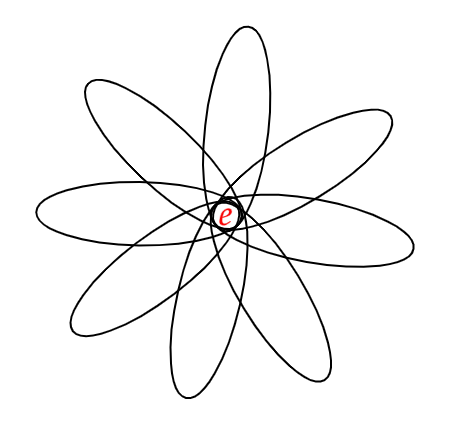
\includegraphics[width=0.3\textwidth]{Figs/1.png}
\end{figure}
\subsubsection{Application of Orbit-Stabiliser Theorem}

The orbit-stabiliser theorem allows us to prove non-trivial results about the structure of finite groups. 

\begin{exma}{\bfs{conjugacy classes}}
Let us consider the action of $G$ (a finite group) on itself by \tb{conjugation}. The orbits under this action are called \tb{conjugacy classes}. Concretely, for $h \in G,$ $$\operatorname{Conj}(h):=\operatorname{Orb}(h)=\left\{g * h * g^{-1} \mid g \in G\right\}.$$

If $C_{1}, \cdots, C_{r} \subset G$ are the
distinct conjugacy classes then we deduce that $|G|=\sum_{i=1}^{r}\left|C_{i}\right|$ and $\left|C_{i}\right|\mid | G |,\forall i \in\{1, \cdots, r\}$ because of Orbit-Stabiliser Theorem.
\end{exma}
\begin{rema}
$|C_i|$ may be different as we have mentioned in \cref{rm:eqec}. Conjugacy classes are not groups.
\end{rema}
\begin{exma}{\bfs{similarity = conjugacy classes}}\label{ex:odnmfv}
If $G=\GL_{n}(\mathbb{R})$, general linear group \cref{def:gl}, then two matrices are in the same conjugacy class if and only if they are similar.
\end{exma}

\begin{defa}{\bfs{Group Center}}
Let $(G, *)$ be a group. The \tb{center} of $G$ is the subgroup
\begin{align*}
Z(G)\coloneqq\{h \in G \mid g * h=h * g, \forall g \in G\}
\end{align*}
\end{defa} 
\begin{proof}
Easy to prove it is a group. And also note that $e$ must be in $Z(G)$.
\end{proof}
\begin{lema}\label{rem:oidnfa}
$G$ is Abelian $\Leftrightarrow$ the center is $G$ itself.
\end{lema}
\begin{thma}\label{thm:odnfad}
Let $G$ be a $p$-group, i.e., a finite group of order $p^{n}$, for $p$ a prime number and $n \in \mathbb{N}$. Then the center is non-tivial: $Z(G)\ne\{e\}$.
\end{thma} 
\begin{proof}
Let $G$ act on itself by conjugation. We know $Z(G)$ is a subgroup. Observe that $h \in Z(G) \Longleftrightarrow \operatorname{Conj}(h)=\{h\} .$ %Recall that $\operatorname{Conj}(e)=\{e\}$, hence $|\operatorname{Conj}(e)|=1 .$ 
Assume that $Z(G)=\{e\} .$ Hence if $h \neq e$ (i.e. $h\notin Z(G)$) then $|\operatorname{Conj}(h)|>1$ (note $h$ is always inside $\operatorname{Conj}(h)$). By the Orbit-Stabiliser Theorem we know that $|\operatorname{Conj}(h)|$ must divide $p^{n}$. Hence $p$ divides $|\operatorname{Conj}(h)| .$ Because the conjugacy classes form a partition of $G$ we deduce that $\exists m \in \mathbb{N}$ such that $p^{n}=1+p m$. This is not possible since it means $p$ and $p$ are coprime, hence $Z(G)$ cannot be trivial.
\end{proof} 


\begin{thma}{\bfs{Sylow's Theorem}}\label{thm:sylow}
 Let $(G, *)$ be a finite group such that $p^{n}$ divides $|G|$, where $p$ is prime. Then there exists a subgroup of size $p^{n}$.
\end{thma}
\begin{rema}{\bfs{Sylow vs. Lagrange}}\label{rm:sylowvslag}
\begin{itemize}
    \item Lagrange's theorem says that if $G$ is a finite group and $H$ is a subgroup then $|H|$ divides $|G| .$ It is not true, in general, that given any divisor of $|G|$ there is a subgroup of that order. We shall see an example of such a group later.
    \item Sylow's Theorem is a partial converse to Lagrange's theorem.
\end{itemize}
\end{rema}
\begin{proof}
Assume that $|G|=p^{n} m$, where $m=p^{r} u$ with $\HCF(p, u)=1 .$ \tb{Our central strategy is to consider a cleverly chosen group action of $G$ and prove one of the stabilizer subgroups has size $p^{n}$.} We'll need to heavily exploit the Orbit-Stabilizer Theorem.

Let $S$ be the \tb{family of all subsets} of $G$ of size $p^{n}$. An element of $S$ is an unordered $p^n$-tuple of \tb{distinct} elements in $G$. There is a natural action of $G$ on $S$ by term-by-term composition on the left:

Let $\omega \in S$. If we fix an arbitrary ordering $\omega=\left\{\omega_{1}, \cdots, \omega_{p^{n}}\right\} \in S$, then for $g\in G$, define $$g(\omega)\coloneqq\left\{g * \omega_{1}, \cdots, g * \omega_{p^{n}}\right\}.$$
In other words, $g$ maps a set to a set.

$\bullet$ We first claim that $\circled{1}:$ $\forall \omega$, $|\Stab(\omega)| \leq p^{n}$. To see this define the function
\begin{align*}
\begin{aligned}
f: \operatorname{Stab}(\omega) & \rightarrow \omega \\
g & \mapsto g * \omega_{1}
\end{aligned}
\end{align*}
We note that $g(\omega)=\omega, \forall g\in\Stab(\omega)$. By the cancellation property for groups $f$ is an injective map. Hence $|\operatorname{Stab}(\omega)| \leq$ $|\omega|=p^{n}$.

$\bullet$ Observe that
\begin{align*}
|S|=\left(\begin{array}{c}
p^{n} m \\
p^{n}
\end{array}\right)=\frac{p^{n} m !}{p^{n} !\left(p^{n} m-p^{n}\right) !}=\prod_{j=0}^{p^{n}-1} \frac{p^{n} m-j}{p^{n}-j}=m \prod_{j=1}^{p^{n}-1} \frac{p^{n} m-j}{p^{n}-j}
\end{align*}
Observe that if $1 \leq j \leq p^{n}-1$ then $j$ is divisible by $p$ at most $n-1$ times, and  that $p^{n} m-j$ and $p^{n}-j$ have the same number of $p$ factors, namely the number of $p$ factor of $j$:

Let $0\le k\le n-1$ be the max such that $p^k|j$. We have $j=p^ka$, with $\HCF(p,a)=1$.
$$p^k|p^nm-j\Leftrightarrow p^k|j\Leftrightarrow p^k|p^n-j$$
We know $p^k|p^n-j$ with $k$ be the max possible integer (easy to get). We need to prove $p^k|p^nm-j$ is also the max possbile one: $p^nm-j=p^nm-p^ka=p^k(p^{n-k}m-a)$, where there is no factor $p$ in $p^{n-k}m-a$ since $\HCF(p,a)=1$.


This means that
\begin{align*}
\prod_{j=1}^{p^{n}-1} \frac{p^{n} m-j}{p^{n}-j}
\end{align*}
has no $p$ factors. Hence $|S|=p^{r} v$, where $\HCF(p, v)=1$.

Now recall that $S$ is the disjoint union of the orbits of our action of $G$ on $S$. Hence there must $\exists\omega \in S$ such that $|\Orb(\omega)|=p^{s} t$, where $s \leq r$ and $\HCF(p, t)=1$. By the \tb{Orbit-Stabilizer Theorem} we know that $|\Stab(\omega)|=p^{n+r-s} \frac{u}{t} .$ Because $|\operatorname{Stab}(\omega)| \in \mathbb{N}$ and $u$ and $t$ are coprime to $p$, we deduce that $\frac{u}{t} \in \mathbb{N}$. Hence $\circled{2}:$ $|\operatorname{Stab}(\omega)| \geq p^{n}$.

For this choice of $\omega \in S, \operatorname{Stab}(\omega)$ is thus a subgroup of size $p^{n}$
\end{proof} 

\begin{lema}\label{lem:ondfdafg}
For any group $G, G / Z(G)$ is cyclic iff $G$ is Abelian, or in otherwords: the quotient $G / Z(G)$ can never be non-trivial cyclic.
\end{lema}
\begin{rema}
Note, $Z(G)$ is \tb{normal} is proved in \cref{rem:idbndadf}.
\end{rema}
\begin{cora}
If $Z$ is contained in $Z(G)$ and $G / Z$ is cyclic, then $G$ is Abelian.
\end{cora}
\begin{proof}
First step: If $G / Z(G)$ is cyclic with generator $x Z(G)$, show that every element of $G$ can be written in the form $x^{a} z$ for some $a \in \mathbb{Z}$ and some element $z \in Z(G)$:

We have that $G / Z(G)$ is cyclic, and so there is an element $x \in G$ such that $G / Z(G)=\gp(x Z(G))$, where $x Z(G)$ is the coset with representative $x$. Now let $g \in G$.
We know that $g Z(G)=(x Z(G))^{m}$ for some $m$, and by definition $(x Z(G))^{m}=x^{m} Z(G)$.
We have that $g Z(G)=x^{m} Z(G)$, and this happens if and only if  $g=x^{m} z$ for some $z \in Z(G)$.

Second step: 
$g, h \in G$ implies that $g=x^{a_{1}} z_{1}$ and $h=x^{a_{2}} z_{2}$, so
\begin{align*}
\begin{aligned}
g h &=\left(x^{a_{1}} z_{1}\right)\left(x^{a_{2}} z_{2}\right) \\
&=x^{a_{1}} x^{a_{2}} z_{1} z_{2} \\
&=x^{a_{1}+a_{2}} z_{2} z_{1} \\
&=\ldots=\left(x^{a_{2}} z_{2}\right)\left(x^{a_{1}} z_{1}\right)=h g .
\end{aligned}
\end{align*}
Third step:  But then from \cref{rem:oidnfa}), it just means $G/Z(G)=\{e\}$.

\end{proof}
\begin{thma}
Showing any group with $p$ or $p^2$ elements are both Abelian. Note, $|Z(G)|=p$ cannot happens.
\end{thma}
\begin{proof}
If the size is $p$, it just means it is cyclic following from \cref{lem:iondfdagtv}. But then \cref{lem:indadf} indicates it is Abelian.

If the size if $p^2$, we then have $Z(G)$ is non-trivial from \cref{thm:odnfad}, so $|Z(G)|=p$ or $p^2$. If $Z(G)=p^2$, it just means $G$ is Abelian following from \cref{rem:oidnfa}. If $|Z(G)|=p$, we have $G/Z(G)$ is cyclic. From \cref{lem:ondfdafg}, we have $G$ is Abelian. But then $Z(G)=G$, so $|Z(G)|=p$ cannot happens.
\end{proof}

\subsection{Finite Symmetric Groups}
As \cref{thm:cayley} (Cayley’s Theorem) shows, if $(G, *)$ is a finite group of order $n$. Then $G$ is isomorphic to a subgroup of $\Sym_{n}$, the symmetric group on $\{1,2 \ldots n\} .$ Hence to properly understand finite groups we must understand these finite symmetric groups.

\begin{lema}
For $n \in \mathbb{N},\left|\Sym_{n}\right|=n !$
\end{lema} 
\subsubsection{Representation of Elements in $\Sym_{n}$: cycles}
We need to think of a way of elegantly representing elements of $\Sym_{n} .$ For $a \in\{1,2 \ldots n\}$ and $\sigma \in \Sym_{n}$, we represent the action of $\sigma$ on $a$ by a cycle:
\begin{align*}
(a b c \ldots f) \text { where } b=\sigma(a), c=\sigma(b) \ldots \sigma(f)=a
\end{align*}
We know that eventually we get back to $a$ because $\sigma$ has finite order. In this way every $\sigma \in \Sym_{n}$ can be written as a \tb{product of disjoint cycles}:
\begin{align*}
\sigma=\left(a_{1} \ldots a_{r}\right)\left(a_{r+1} \ldots a_{s}\right) \ldots\left(a_{t+1} \ldots a_{n}\right)
\end{align*}

This representation is \tb{unique up to internal shifts and reordering the cycles.}

\begin{exma}
Let $n=5$ then $\sigma=(123)(45)$ corresponds to
\begin{align*}
\begin{aligned}
1 & \longrightarrow 2 \\
2 & \longrightarrow 3 \\
\sigma: 3 & \longrightarrow 1 \\
4 & \longrightarrow 5 \\
5 & \longrightarrow 4
\end{aligned}
\end{align*}
\end{exma} 
If an element is fixed by $\sigma$ we omit it from the notation.
\begin{exma}
Let $n=5$ then $\sigma=(523)$ corresponds to
\begin{align*}
\begin{aligned}
1 & \longrightarrow 1 \\
2 & \longrightarrow 3 \\
\sigma: 3 & \longrightarrow 5 \\
4 & \longrightarrow 4 \\
5 & \longrightarrow 2
\end{aligned}
\end{align*}
\end{exma}
This notation makes it clear how to compose two permutations. 
\begin{exma}
Let $n=5$ and $\sigma=(23), \tau=(241)$, then $\tau \sigma=(241)(23)=(1234)$ and $\sigma \tau=(23)(241)=(1324) .$ Observe
that composition is on the left when composing permutations.
\end{exma} 
\begin{rema}
This example also shows that in general $\Sym_{n}$ is \tb{not Abelian.}
\end{rema}
\begin{defa}{\bfs{Cycle Structure}}
Hence, given $\sigma \in \Sym_{n}$, we naturally get a well-defined partition of $n$, taking the lengths of the disjoint cycles appearing in $\sigma$. This is call the \tb{cycle structure} of $\sigma$.
\end{defa}
\begin{rema}{\bfs{explanation}}
Cycle structure is a set of numbers (not a collection of set). There is no order since any order is okay (corresponds to reordering the cycles).
\end{rema}
\begin{lema}
Let $\sigma \in \Sym_{n}$ decompose as the disjoint product of cycles of length $n_{1}, . . n_{m}$ (so $\left.\sum n_{i}=n\right) .$ Then $\ord(\sigma)=\LCM\left(n_{1}, \ldots n_{m}\right)$.
\end{lema} 
\begin{proof}
Let $\sigma=\left(a_{1}, \cdots, a_{r}\right)\left(a_{r+1}, \cdots, a_{s}\right) \cdots\left(a_{t+1}, \cdots, a_{n}\right)$, be a representation of $\sigma$ as the
disjoint product of cycles. We may assume that $r=n_{1}$, etc, without any loss of generality. Observe that \tb{a cycle of length $m \in \mathbb{N}$ must have order $m$ in $\Sym_{n}.$} Also recall that if $G$ is a finite group then for any $d \in \mathbb{N}, x \in G, x^{d}=e \Longleftrightarrow$ $\ord(x) \mid d$. Also observe that for all $d \in \mathbb{N}, \sigma^{d}=\left(a_{1}, \cdots, a_{r}\right)^{d}\left(a_{r+1}, \cdots, a_{s}\right)^{d} \cdots\left(a_{t+1}, \cdots, a_{n}\right)^{d}$. Thus we know that $\sigma^{d}=e$
$\Longleftrightarrow n_{i} \mid d, \forall i$. The smallest value $d$ can take with this property is $\LCM\left(n_{1}, \ldots n_{m}\right)$. 
\end{proof} 
\begin{thma}
Two permutations are \tb{conjugate} in $\Sym _{n}$ if and only if they have the \tb{same cycle structure}.
\end{thma}
\begin{proof}
Let $\sigma, \tau \in \operatorname{Sym}_{n}$ have the same cycle structure. Hence we may represent both in the form:
\begin{align*}
\sigma=\left(a_{1}, \cdots, a_{r}\right)\left(a_{r+1}, \cdots, a_{s}\right) \cdots\left(a_{t+1}, \cdots, a_{n}\right)
\end{align*}
\begin{align*}
\tau=\left(b_{1}, \cdots, b_{r}\right)\left(b_{r+1}, \cdots, b_{s}\right) \cdots\left(b_{t+1}, \cdots, b_{n}\right)
\end{align*}
Define $\alpha \in \Sym_{n}$ such that $\alpha\left(a_{i}\right)=b_{i},\forall i .$ By construction $\alpha^{-1} \tau \alpha=\sigma .$ Going through the above process in reverse, the converse is clear.
\end{proof} 

\begin{cora}\label{cor:oidnfacvb}
Conjugacy classes in  $\Sym_{n}$ are indexed by cycle structures (i.e. partitions of $n$ ).
\end{cora} 
\begin{proof}
Immediate from the above.
\end{proof}
\subsubsection{Transposition, Even and Odd Permuation}
\begin{defa}{\bfs{Transposition}}
A transposition is a cycle of length 2 .
\end{defa} 
Observe that we can write \tb{any cycle as a product of transpositions}:
a computation shows that
\begin{align}
\left(a_{1}, a_{2}, \cdots, a_{n}\right)=\left(a_{1}, a_{n}\right)\left(a_{1}, a_{n-1}\right) \cdots\left(a_{1}, a_{3}\right)\left(a_{1}, a_{2}\right) \label{eq:cyc_2_tran}
\end{align}

Hence any permutation $\sigma \in \operatorname{Sym}_{n}$ may be written as the (not necessarily disjoint) product of transpositions. This representation is non-unique as the following shows:
e.g. $n=6, \sigma=(1, 2, 3)=(1,3)(1,2)=(4,5)(1,3)(4,5)(1,2)$.
\begin{rema}
Notice that in the above example, both expressions involve an \tb{even} number of transpositions.
\end{rema}

\begin{defa}{\bfs{Sign: even or odd}}
Let us call $\sigma$ \tb{even} if there are an \tb{even} number of \tb{even} length cycles (once expressed as a disjoint product); let us call $\sigma$ \tb{odd} if there are an \tb{odd} number of \tb{even} length cycles. We also define the \tb{sign} of $\sigma$, denoted $\operatorname{sgn}(\sigma)$, to be $+1$ or $-1$ depending on whether $\sigma$ is even or odd.
\end{defa} 
\begin{rema}
This indeed is a definition because the disjoint product cycles representation is unique (up to internal shifts and reordering the cycles)
\end{rema}
\begin{rema}{\bfs{equivalent statements}}
\begin{itemize}
    \item\tb{ even:} number of product of transpositions is even
    \item \tb{odd:} number of product of transpositions is odd.
\end{itemize}
For one cycle, if it has even length, it can be rewritten as an odd number of transpositions.
Two even cycle $\Rightarrow$ an even number of transpositions. So an \tb{odd} number of \tb{even} length cycles $\Rightarrow$ an \tb{odd} number of transpositions.

Why this equivalent statement is also a definition?  If we take \cref{eq:cyc_2_tran} as the canonical decomposition, of course we make the above as a definition. In the general case, $\sigma \in \operatorname{Sym}_{n}$ may be written as some arbitrary product of  transpositions, we need the last paragraph below in the proof of \cref{thm:eqffd}.
\end{rema}

\begin{thma}\label{thm:eqffd}
Let $\sigma \in$  $\Sym_{n}$ be expressed as the product of transpositions in two potentially different ways. If the first has $m$ transpositions and the second has $n$ transpositions then $2 \mid(m-n)$.
\end{thma}
\begin{rema}\bfs{comparison of determinant and similarity of matrix}
\begin{enumerate}
    \item\label{dfda:dfcg} Another proof of \cref{thm:eqffd} use an identity matrix and its determinant, switch ($i$,$j$) means switch two rows. Determinant must be either even or odd. It cannot be even and odd at the same time.
    \item Also note conjugacy classes plays the role of the similarity in $\GL_n(\Real)$  as shown in \cref{ex:odnmfv}. Similarity in $\GL_n(\Real)$  will guarantees the \tb{same sign of determinant}.
    \item Here for conjugacy classes in $\Sym_n$, we also have similar properties as indicated by \cref{cor:oidnfacvb}. This is also why \cref{dfda:dfcg} can prove \cref{thm:eqffd}. 
    \item \tb{Key}: Conjugacy classes in $\Sym_n$ is a special case of similarity where the \tb{domain is only permutation matrix.}
\end{enumerate}

\end{rema}
\begin{proof}

First notice that a cycle of length $r$ can be written as the product of $r-1$ transpositions by \cref{eq:cyc_2_tran}. 
Consider how sign changes when we multiply by a transposition $(1, i)$. We have two cases:
\begin{enumerate}[(1).]
    \item 1 and $i$ occur in the same cycle in $\sigma .$ Without loss of generality we consider $(1,2, \cdots, i$, $\cdots r$ ) as being in $\sigma$.
\begin{align*}
(1, {i})(1,2, \cdots, i, \cdots, r)=(1,2, \cdots, i-1)(i, i+1, \cdots, r)
\end{align*}
If $r$ is even then either we get two odd length cycles or two even length cycles. If $r$ is odd then exactly one of the cycles on the right is even length. In either case, $\operatorname{sgn}((1, i) \sigma)=-\operatorname{sgn}(\sigma)$
\item 1 and $i$ occur in distinct cycles. Again, without loss of generality we may assume that $(1 \cdots i-1)(i \cdots r)$ occurs in $\sigma .$ In this case
\begin{align*}
(1, {i})(1,2, \cdots, i-1)(i, \cdots, r)=(1, \cdots ,r)
\end{align*}
In either of the cases $r$ even or odd, we see that the number of even length cycles must drop or go up by one. Hence $\operatorname{sgn}((1, i) \sigma)=-\operatorname{sgn}(\sigma)$ as in case 1 .


\end{enumerate}


We deduce that multiplying on the left by a transposition changes the sign of our permutation. The identity must have sign 1 , hence by induction we see that the \tb{$\circled{1}$ (existence): product of an odd number of transpositions has sign $-1$, and the product of an even number of transpositions has sign 1.} 

Note that if we write any product of transpositions then we can immediately write down an inverse by reversing their order. Let us assume that we can express $\sigma$ as the product of transpositions in two different ways, one with an odd number and one with an even number. Hence we can write down $\sigma$ as the product of evenly many transpositions and $\sigma^{-1}$ as a product of an odd number of transpositions. Thus we can write $e=\sigma * \sigma^{-1}$ as a product of an odd number of transpositions. \tb{$\circled{2}$ (uniqueness)}: This is a contradiction as $\operatorname{sgn}(e)=1$. 
\end{proof}

\begin{rema}
We should observe that from the proof of the above we see that $$\forall \sigma, \tau \in \operatorname{Sym}_{n}, \operatorname{sgn}(\sigma \tau)=\operatorname{sgn}(\sigma) \operatorname{sgn}(\tau) .$$

Because $\operatorname{sgn}(e)=1$ we deduce that $\operatorname{sgn}(\sigma)=\operatorname{sgn}\left(\sigma^{-1}\right)$ for all $\sigma \in \Sym_{n} .$
\end{rema}

In particular this shows that the set of even elements of $\Sym_{n}$ contains the identity and is closed under composition and taking inverse. Hence we have the following:

\begin{defa}{\bfs{Alternating Group}}
The subgroup of $\Alt_{n} \subset$  $\Sym_{n}$ consisting of \tb{even} elements is called the \tb{alternating group} of rank $n$.
\end{defa}
\begin{rema}
So $\Alt_{n}$ is the permutation matrix with positive determinant.
\end{rema}
Observe that $\Alt_{n}$ contains all $3$-cycles (cycles of length $3$). Further more we have
\begin{lema}
$\Alt_{n}$ is generated by $3$-cylces.
\end{lema}
\begin{proof}
As any element of $\Alt_{n}$ can be written as the product of transpositions, we only have to do it for the product of two (because of even) transpositions. There are two cases:
\begin{enumerate}
    \item $(i,j)(k,l)=(k,i,l)(i,j,k) .$
    \item $(i,j)(i,k)=(i,k,j)$.
\end{enumerate} 
\end{proof}
\begin{lema}
$\left|\Alt_{n}\right|=\frac{n !}{2}$
\end{lema}
\begin{proof}
Recall that $\left|\Sym_{n}\right|=n !$, hence we just need to show that $\left(\operatorname{Sym}_{n}: \Alt_{n}\right)=2$. Let $\sigma, \tau \in \Sym_{n}$. Recall that
\begin{align*}
\sigma \Alt_{n}=\tau \Alt_{n} \Longleftrightarrow \sigma^{-1} \tau \in \Alt_{n}
\end{align*}
$\operatorname{But} \operatorname{sgn}\left(\sigma^{-1} \tau\right)=\operatorname{sgn}(\sigma) \operatorname{sgn}(\tau)$, hence
\begin{align*}
\sigma \Alt_{n}=\tau \Alt_{n} \Longleftrightarrow \operatorname{sgn}(\sigma)=\operatorname{sgn}(\tau)
\end{align*}
Hence $\Alt_{n}$ has two left cosets in $\Sym_{n}$, one containing even permutations and one odd permutations.
\end{proof} 
\begin{rema}
The alternating groups for $n \geq 5$ have a very special property called \tb{simple} \cref{def:simple}.
\end{rema}

\subsection{Symmetry of Sets with Extra Structure}
Let $S$ be a set and $\Sigma(S)$ its permutation group. The permutation group  $\Sigma(S)$ completely ignores the fact that there may be extra structure on $S$.

For vector space $\mathbb{R}^{n}$:
\begin{itemize}
    \item The permutation group $\Sigma\left(\mathbb{R}^{n}\right)$ does not take this into account and elements do not need to be a linear invertible mapping.
    \item $\GL_{n}(\mathbb{R})\subset \Sigma\left(\mathbb{R}^{n}\right)$ only includes linear invertible mapping (permutations).  These are permutations which preserve the vector space stucture under "addition" and "multiplication".
\end{itemize}
\subsubsection{Symmetry in Euclidean Space: isometry, symmetry group}
\begin{defa}
Given $n \in \mathbb{N}, n$-dimensional Euclidean space is the vector space $\mathbb{R}^{n}$ equipped with the standard inner product (the dot product). 

\centerline{Concretely, if $\boldsymbol{x}=\left(\begin{array}{c}x_{1} \\ \vdots \\ x_{n}\end{array}\right), \boldsymbol{y}=\left(\begin{array}{c}y_{1} \\ \vdots \\ y_{n}\end{array}\right) \in \mathbb{R}^{n}$ then $\langle\boldsymbol{x}, \boldsymbol{y}\rangle:=x_{1} y_{1}+\cdots+x_{n} y_{n}$}
\end{defa} 
\begin{defa}{\bfs{Euclidean Distance}}\label{def:euc_dis}
The Euclidean distance between $\boldsymbol{x}$ and $\boldsymbol{y}$ in $\mathbb{R}^{n}$ is
\begin{align*}
d(\boldsymbol{x}, \boldsymbol{y}):=\sqrt{\langle\boldsymbol{x}-\boldsymbol{y}, \boldsymbol{x}-\boldsymbol{y}\rangle}
\end{align*}
and the  norm (length) of $\boldsymbol{x}$ is:
\begin{align*}
||\boldsymbol{x}||:=d(\boldsymbol{x}, \boldsymbol{0})
\end{align*}
\end{defa}
\begin{defa}{\bfs{Isometry}}
 An isometry of $\mathbb{R}^{n}$ is a map of sets $f: \mathbb{R}^{n} \rightarrow \mathbb{R}^{n}$ (\tb{not necessarily linear}) such that $\forall \boldsymbol{x}, \boldsymbol{y} \in \mathbb{R}^{n}, d(\boldsymbol{x}, \boldsymbol{y})=d(f(\boldsymbol{x}), f(\boldsymbol{y}))$, where $d$ is the Euclidean distance function. The collection of all isometries of $\mathbb{R}^{n}$ is denoted by
$\operatorname{Isom}\left(\mathbb{R}^{n}\right)$.
\end{defa}
\begin{rema}{\bfs{some facts about isometry}} We statement the following without proof. See also \cite[page 85 and 320 ]{horn2012matrix} and the supp material.
\begin{itemize}
    \item Under the \tb{Euclidean distance} in \cref{def:euc_dis}, every isometry of $\mathbb{R}^{n}$ is a composition of an origin fixing isometry (linear isometry) and a translation. We may call the composition as the \tb{affine mapping} written as $f(\boldsymbol{x})=\boldsymbol{A} \boldsymbol{x}+\boldsymbol{y}$:
    \begin{enumerate}
        \item \tb{origin fixing isometry:} $f(\boldsymbol{x})=\boldsymbol{A} \boldsymbol{x}$, where $\boldsymbol{A}$ must be \tb{orthogonal}.
        \item \tb{translation:} $f(\boldsymbol{x})= \boldsymbol{x}+\boldsymbol{y}$ for some $\boldsymbol{y}\in \Real^n$
    \end{enumerate}
    \item The composition of any two isometries is an isometry.
    \item All isometries are bijective and their inverses are isometries. This means $ \operatorname{Isom}\left(\mathbb{R}^{n}\right)$ is a \tb{subgroup} of $\Sigma\left(\mathbb{R}^{n}\right) .$
    \item Give that $f(\boldsymbol{x})=\boldsymbol{A} \boldsymbol{x}$ where $\boldsymbol{A}$ is \tb{orthogonal}. We then have that the \tb{positive scalar multiples of the Euclidean norm} are the only \tb{unitarily invariant norms} on $\Real^n$.
\end{itemize}
\end{rema}
\begin{defa}{\bfs{Symmetry Group}}
 Let $X \subset \mathbb{R}^{n}$ be a subset (not necessarily a subspace). We define the \tb{symmetry group} of $X$ to be the subgroup $\operatorname{Sym}(X) \subset \operatorname{Isom}\left(\mathbb{R}^{n}\right)$ with the property that $f \in \operatorname{Sym}(X)$ if and only if $f$ permutes $X$:
 $$\Sym(X) = \Sigma(X)\cap \Isom(\Real^n) $$
\end{defa}
\begin{rema}\label{rm:somegroupsrelateion} Note in the following $\Sigma(X)$ in general is \tb{not} a subset of $\operatorname{Isom}\left(\mathbb{R}^{n}\right)$.
\begin{itemize}
    \item Note we have $\operatorname{Sym}(X) \subset \operatorname{Isom}\left(\mathbb{R}^{n}\right)\subset \Sigma(\Real^n)$.
    \item Define $\operatorname{Isom}^*\left(\mathbb{R}^{n}\right)\coloneqq\{f(\boldsymbol{x})=\boldsymbol{A} \boldsymbol{x}, \boldsymbol{A} \text{ is orthogonal}\}$. We have $\operatorname{Isom}^*\left(\mathbb{R}^{n}\right) \subset \GL_n(\Real^n) \subset \Sigma(\Real^n)$. 
    \item $\operatorname{Sym}(X) \subset \Sigma(X)\subset \Sigma(\Real^n)$.
    \item  $\operatorname{Sym}(X)$ (Symmetry Group) vs.  $\Sym_k$ (Permuation Group, $\Sigma$): $\operatorname{Sym}(X) \subset \Sym_k$ for finite $|X|=k$.
\end{itemize}

\end{rema}
There is a natural action of $\operatorname{Sym}(X)$ on the set $X$, coming from the fact there is a natural homomorphism $\operatorname{Sym}(X) \rightarrow \Sigma(X)$.
homomorphism $g$ :
\begin{align*}
\Sym(X) &\rightarrow \Sigma(\mathbb{R}^n)\\
f &\mapsto f
\end{align*}
$\operatorname{Sym}(X)$ measures how much symmetry $X$ has. The more symmetric $X$, the larger $\operatorname{Sym}(X)$.

\subsubsection{Dihedral Group in $\Real^2$}

\begin{defa}{\bfs{Dihedral Group: regular $m$-gon}}
 Let $m \in \mathbb{N}$ and $X \subset \mathbb{R}^{2}$ be a regular $m$-gon centered at the origin. We call the symmetry group of $X$ the \tb{dihedral group} of rank $m$, and we denote it by $D_{m}$.
\end{defa}
\begin{rema}{\bfs{$D_{m}$: subgroup of orthogonal matrices}}
First observe that every element of $D_{m}$ must fix the center of $X$ (the origin). Thus we may view $D_{m}$ as a subgroup of the group of $2 \times 2$ orthogonal matrices. We shall not take this approach here.
\end{rema}
\begin{enumerate}
    \item $f \in D_{m}$ is a group action \tb{faithfully} on set  $X$: see Example 1 in \cref{exm:act} with a $D_{m}$ being a subgroup of $\Sigma(X)$
    \item $f \in D_{m}$ is a group action \tb{transitive} on set  $X$: since only one orbit = set of verticals . 
\end{enumerate}


 Hence $D_{m}$ can naturally by identified with a subgroup of $\Sym_{m} .$ Let $\sigma$ be the rotation by $\frac{2 \pi}{m}$ clockwise about the origin. All possible \tb{rotational symmetries} are generated by $\sigma$, namely
\begin{align*}
\operatorname{Rot}_{m}=\left\{e, \sigma, \sigma^{2}, \cdots, \sigma^{m-1}\right\} \subset D_{m}
\end{align*}
\begin{rema}
 $\operatorname{Rot}_{m}$ a \tb{subgroup} and is cyclic of order $m$.
\end{rema}

Given a vertex $a, \operatorname{Stab}(a)=\{e, \tau\}$, where $\tau$ is the reflection through the straight line containing $a$ and the origin. We have  $\left|D_{m}:\Stab(a)\right|=m$ since the maximum possible value is $m$ and we can achieve it. Note this is because \cref{lem:bi_g_stab}, and for $\Orb(s)$ is set of all vertex.

By the Orbit-Stabilizer theorem $\left|D_{m}\right|=2 m$, hence $\left(D_{m}:\operatorname{Rot}_{m}\right)=2$. We deduce that
\begin{align*}
D_{m}=\operatorname{Rot}_{m} \coprod \tau \operatorname{Rot}_{m}
\end{align*}
The left coset $\tau \operatorname{Rot}_{m}$ is precisely the set of reflective symmetries. Hence every element of $D_{m}$ can be written in the form $\sigma^{k}$ (if a rotation) or $\tau \sigma^{k}$ (if a reflection). The group structure is completely determined by the following properties
\begin{itemize}
    \item $\operatorname{ord}(\sigma)=m$
    \item  $\operatorname{ord}(\tau)=2$
    \item $\tau \sigma=\sigma^{-1} \tau$ (consider the action on the vertices)
\end{itemize}
Observe that the third property implies that $D_{m}$ is \tb{not Abelian.} Here is a picture for $n=3$.
\begin{figure}[h]
\caption{$D_3$}
\centering
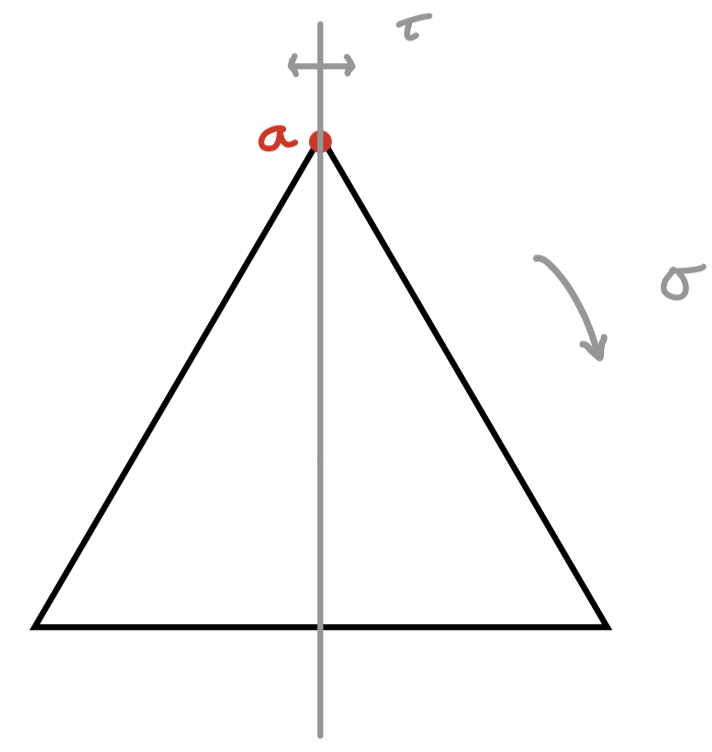
\includegraphics[width=0.25\textwidth]{Figs/fig_Dihedral.png}
\end{figure}

\subsubsection{The Cube in $\mathbb{R}^{3}$}
Let $X \subset \mathbb{R}^{3}$ be a solid cube centered at the origin. Again, elements of $\operatorname{Sym}(X)$ must fix the origin, hence, if we wished, we could identify $\operatorname{Sym}(X)$ with a subgroup of the group of $3 \times 3$ orthogonal matrices.

Again $\operatorname{Sym}(X)$ acts faithfully and transitively on the vertices. If $a \in X$ is a vertex, then  $\Stab(a)$ can naturally be identified with $D_{3}$ (see below figure, not $D_6$) which has size $6$ . Hence, by the Orbit-Stabilizer theorem, $|\operatorname{Sym}(X)|=48$ since $\Orb(s)=8$.

The same logic applies to $\operatorname{Rot}_{\square}$, \tb{the rotational symmetries}, although the stabilizer of $a$ now has size 3 . This tells us that $\left|\operatorname{Rot}_{\square}\right|=24$.
\begin{figure}[h]
\centering
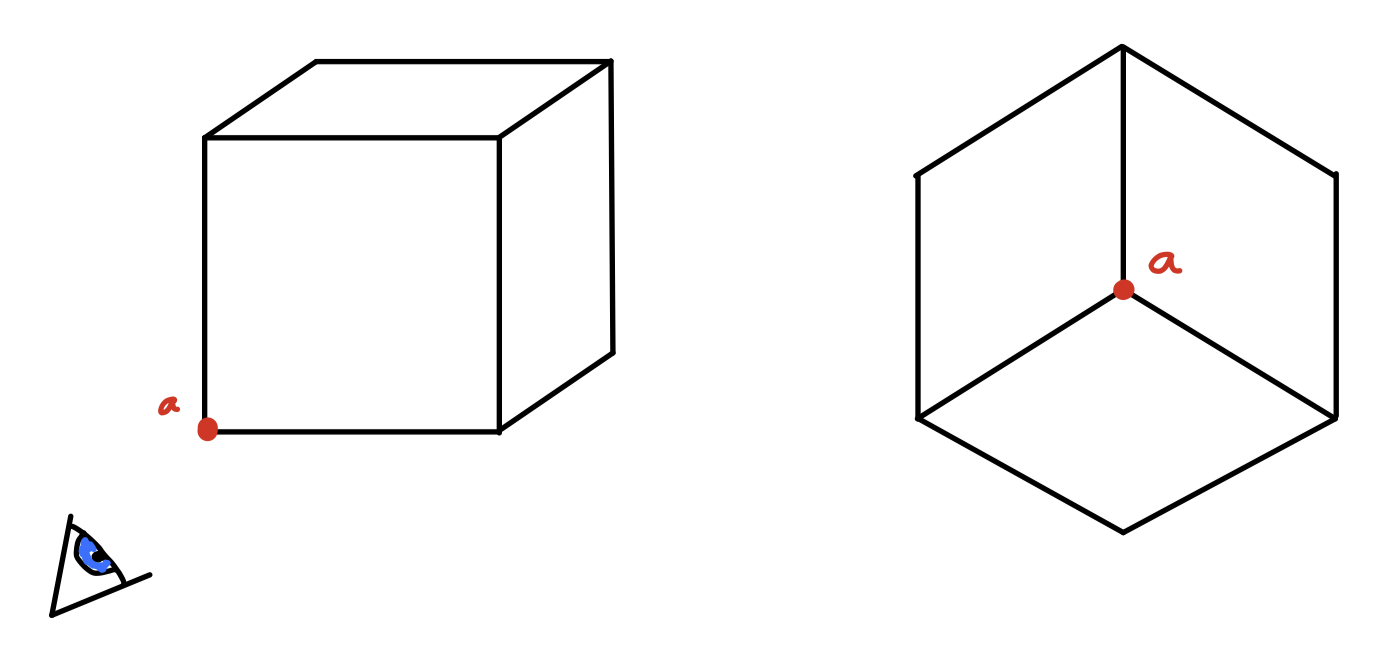
\includegraphics[width=0.5\textwidth]{Figs/cube1.png}
\end{figure}

If $\tau \in \operatorname{Sym}(X)$ is the symmetry sending $\boldsymbol{x}$ to $-\boldsymbol{x}$ (this is not a rotation), then again
\begin{align*}
\operatorname{Sym}(X)=\operatorname{Rot}_{\square} \coprod \tau\operatorname{Rot}_{\square}
\end{align*}
It can be shown that $\tau \sigma=\sigma^{-1} \tau$ for all $\sigma \in \operatorname{Rot}_{\square}$. Thus it remains to determine the group structure of $\operatorname{Rot}_{\square}$

Color the vertices with four colors, making sure that opposite vertices have the same color (see below figure). Rotational symmetries act on this set of four colors, inducing a homomorphism from $\operatorname{Rot}_{\square}$ to $\Sym_{4} .$ Given any two colors, it is possible to transpose them (leaving the others fixed) by a rotation. Because $\Sym_{4}$ is generated by transpositions, the induced homormorphism $\operatorname{Rot}_{\square}\rightarrow \Sym_{4}$ must be surjective. However, $\left|\operatorname{Rot}_{\square}\right|=24=4 !=$ $\mid$ $\Sym_{4} \mid .$ Hence it must be an isomorphism (because of bijective). 
\begin{lema}
We deduce that $\operatorname{Rot}_{\square}$ is isomorphic to $\Sym_{4}$.
\end{lema}
\begin{figure}[h]
\centering
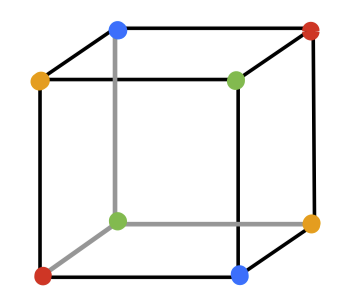
\includegraphics[width=0.2\textwidth]{Figs/cube2.png}
\end{figure}


\subsubsection{One Interesting Question}
Let $(G, *)$ be an abstract group. When is it true that we can find $X \subset \mathbb{R}^{n}$, for some $n \in \mathbb{N}$ such that
\begin{align*}
G \cong \operatorname{Sym}(X) ?
\end{align*}
Less formally, when can an abstract group be realised in geometry? 
\begin{rema}
I think the answer is no with the group being $\Sigma(\Real^n)$ in \cref{rm:somegroupsrelateion}.
\end{rema}

\subsection{Normal Subgroups and Isomorphism Theorems}
\begin{enumerate}
    \item In linear algebra, we study the linear maps $\boldsymbol{A}$, and not the vector spaces themselves. The structure preserving maps between vector spaces are more interesting than the spaces themselves.
    \item Philosophically it's saying that an object in isolation is uninteresting; it's how it relates to what's around it that matters.
\end{enumerate} 
In this section, we study \tb{homomorphisms between abstract groups}.

Let $G$ and $H$ be two groups. We'll suppress the $*$ notation as it will always be obvious where composition is taking place. Let $e_{G}$ and $e_{H}$ be the respective identity elements. Recall that a homomorphism from $G$ to $H$ is a map of sets $f: G \rightarrow H$ such that $\forall x, y \in G$, $f(x y)=f(x) f(y)$
\subsubsection{Kernel and Image: subgroups}
\begin{defa}{\bfs{Kernel and Image}}
 Given $f: G \rightarrow H$ a homomorphism of groups, we define the \tb{kernel} of $f$ to be:
\begin{align*}
\operatorname{Ker}(f):=\left\{x \in G \mid f(x)=e_{H}\right\}
\end{align*}
We define the \tb{image} of $f$ to be:
\begin{align*}
\operatorname{Im}(f):=\{y \in H \mid \exists x \in G \text { such that } f(x)=y\}
\end{align*}
\end{defa} 
\begin{lema}
Given a homomorphism $f: G \rightarrow H, \operatorname{Ker}(f) \subseteq G$ and $\Ima(f) \subseteq H$ are subgroups.
\end{lema} 
\begin{proof}
First we will show true for $\operatorname{Ker}(f)$ :
\begin{enumerate}
    \item $f\left(e_{G}\right)=e_{H} \Rightarrow e_{G} \in \operatorname{Ker}(f)$.
    \item  Suppose $x, y \in\operatorname{Ker}(f)$. Then $f(x y)=f(x) f(y)=e_{H} \Rightarrow x y \in \operatorname{Ker}(f)$.
    \item Given $x \in \operatorname{Ker}(f), f\left(x^{-1}\right)=e_{H}^{-1}=e_{H} \Rightarrow x^{-1} \in \operatorname{Ker}(f)$.
\end{enumerate}
Now we will show that $\operatorname{Im}(f)$ is a subgroup:
\begin{enumerate}
    \item $f\left(e_{G}\right)=e_{H}$ so $e_{H} \in \operatorname{Im}(f)$.
    \item $f(x y)=f(x) f(y), \forall x, y \in G$ so $\operatorname{Im}(f)$ is closed under composition.
    \item Note that $f(x)^{-1}=f\left(x^{-1}\right) \Rightarrow y \in \operatorname{Im}(f) \Rightarrow y^{-1} \in \operatorname{Im}(f)$.
\end{enumerate}
\end{proof} 

\begin{lema}\label{lem:hom_bi_e}
A homomorphism $f: G \rightarrow H$ is injective if and only if $\Ker(f)=\{e_G\}$ .
\end{lema} 
\begin{proof}
$f$ injective $\Rightarrow \operatorname{Ker}(f)=\left\{e_{G}\right\}$ is easy. Now assume $\operatorname{Ker}(f)=\left\{e_{G}\right\}$. Suppose $x, y \in G$ such that $f(x)=f(y)$
\begin{align*}
\begin{aligned}
f(x)=f(y) & \Rightarrow f(x) f(y)^{-1}=e_{H} \\
& \Rightarrow f(x) f\left(y^{-1}\right)=e_{H} \\
& \Rightarrow f\left(x y^{-1}\right)=e_{H} \\
& \Rightarrow x y^{-1}=e_{G} \\
& \Rightarrow x=y
\end{aligned}
\end{align*}
Thus $f$ is injective.
\end{proof} 
\subsubsection{Normal Group}\label{sssec:normal}
Let $x H, y H \in G / H$ be two left cosets. Recall that $x$ and $y$ are not necessarily unique. The only obvious way for combining $x H$ and $y H$ would be to form $(x y) H .$ In general this is \tb{not} well defined. It will depend on the choice of $x$ and $y$. In the case $G=\mathbb{Z}$ and $m \mathbb{Z}=H$, we know for any $x$ and $y$, we can define the binary operator and makes $G/m \mathbb{Z}$ a well defined new group. 

What's the answer for the general case?  We need $H$ to be a \tb{normal} group!

\begin{defa}{\bfs{Normal Group}}
 We call a subgroup $H \subseteq G$ \tb{normal} if it satisfies equivalently any one of the following condition 
 \begin{itemize}
     \item $g H g^{-1}\coloneqq\left\{g h g^{-1} \mid g\in G, h \in H\right\}=H$;  
     \item  $\forall g\in G$, and $\forall h \in H$, $g h g^{-1}\in H$;
     \item left coset equals right coset for $\forall g \in G$: $gH=Hg$;
     \item  the union of conjugacy classes of $G$ equals $H$, i.e., if $H=\bigcup_{h\in H}\Conj(h)$;
     \item Any two elements commute regarding the normal subgroup membership relation: for all $g, h \in G, g h \in H$ if and only if $h g \in H$
 \end{itemize}
 We denote \tb{normal subgroup} by $H \triangleleft G .$
\begin{proof}
We only show the equivalence between last one and others.

Assume the last one is true. For any $h\in H$, we have $hg^{-1}g=h\in H$ for any $g\in G$, so $ghg^{-1}\in H$.
% We get $g^{-1}h^{-1}\in H$, so $ghg^{-1}h^{-1}\in H$. For any $h\in H$, we then have $ghg^{-1}\in H$.


Assume $\forall g\in G$, and $\forall h \in H$, $g h g^{-1}\in H$. If $ab\in H$ for a pair of elements $a,b\in G$. We have $b^{-1}a^{-1}\in H$, so $a^{-1}(b^{-1}a^{-1})a\in H$. That means $a^{-1}b^{-1}\in H$. So $ba\in H$.
\end{proof}

\end{defa} 
\begin{rema}{\bfs{explanation}} \label{rem:idbndadf}

\begin{enumerate} 
    \item \begin{enumerate}
        \item The definition of normal group is not saying that given $g \in G$ and $h \in H$, then $\mathrm{ghg}^{-1}=h$. It is merely saying that  $ghg^{-1} \in H .$ 
\item The definition of  group center means: if $h\in Z(G)$, $\mathrm{ghg}^{-1}=h$ for all $g\in G$.
    \end{enumerate}
\item Note here  $H=\{ghg^{-1}\mid g=e_G,h\in H\}$. So for all subgroup $H$, we have  $H\subseteq gHg^{-1}$.
 \item normal subgroup vs. conjugacy vs.  group center:
 \begin{enumerate}
 \item[$\bullet$] Recall:  $\operatorname{Conj}(h):=\operatorname{Orb}(h)=\left\{g * h * g^{-1} \mid g \in G\right\}$; $Z(G)\coloneqq\{h \in G \mid g * h=h * g, \forall g \in G\}$
 \item  Observe that $h \in Z(G) \Longleftrightarrow \operatorname{Conj}(h)=\{h\} .$
      \item A  subgroup is normal \tb{if} the union of conjugacy classes of $G$ equals $H$, i.e., if $H=\bigcup_{h\in H}\Conj(h)$. 
    %   \item 
    \item \tb{Group center is a normal subgroup}. And group center is more restrict than normal subgroup as we have mentioned in 1.
 \end{enumerate}
   
    \item \tb{If $G$ is Abelian, every subgroup is normal as $g h g^{-1}=h, \forall g, h \in G$.}
\end{enumerate} 
\end{rema} 
\begin{exma}{\bfs{non-normal group}}
 Let $G=\Sym_{3}, H=\{e,(1,2)\} .$ Then $(13)(12)(13)=(23) \notin H$
Hence $H$ is not normal in $\Sym_{3}$, so in general not all subgroups of a group are normal.
\end{exma}
\begin{thma}{\bfs{Kernal of Homomorphism is Normal}}\label{eq:kernnorm}

Let $G$ and $H$ be two groups. Let $f: G \rightarrow H$ a homomorphism. Then $\operatorname{Ker}(f) \subset G$ is a \tb{normal subgroup}.
\end{thma} 
\begin{proof}
Let $h \in \operatorname{Ker}(f)$ and $g \in G$. Then $f\left(g h g^{-1}\right)=f(g) f(h) f\left(g^{-1}\right)=f(g) e_{H} f(g)^{-1}=$
$e_{H} \Rightarrow g h g^{-1} \in \Ker(f)$
\end{proof} 
\begin{rema}
In general $\operatorname{Im}(f) \subset H$ is \tb{not} normal.
\end{rema}

\begin{defa}{\bfs{Simple}}\label{def:simple}
 We say a group $G$ is \tb{simple} if its only normal subgroups are
$\{e\}$ and $G$
\end{defa} 
\begin{exma}
Groups of prime order are trivially simple by Lagrange's theorem. As we shall see later simple groups are the \tb{core building blocks of groups theory.}
\end{exma}
\begin{rema}
Also recall that  a finite group  $G$ with order $p^{n}$, for $p$ a prime number and $n \in \mathbb{N}$. Then the center is non-tivial: $Z(G)\ne\{e\}$.
\begin{enumerate}
    \item Additionally, if $G$ is not Abelian, the group center, which is normal, is not $G$ (and nontrivally). So $G$ is then not simple.  \item Additionally, if $G$ is Abelian, the center is $G$. Later we will see in this case $G$ is possibly not simple as shown in \cref{cor:dfdfadf}.
\end{enumerate}
\end{rema}
The importance of normal subgroups can be seen in the following:
\begin{lema}
Let $H \subseteq G$ be a normal subgroup. Then the binary operation:
\begin{align*}
\begin{gathered}
G / H \times G / H \rightarrow G / H \\
(x H, y H) \mapsto(x y) H
\end{gathered}
\end{align*}
is well defined.
\end{lema}
\begin{proof}
As usual the problem is that that coset representatives are not unique and thus we could have two representatives giving different maps. Thus our goal is to show:
$\forall x_{1}, x_{2}, y_{1}, y_{2} \in G$ such that $x_{1} H=x_{2} H$ and $y_{1} H=y_{2} H$, then $\left(x_{1} y_{1}\right) H=\left(x_{2} y_{2}\right) H$.
By assumption we know $x_{1}^{-1} x_{2}, y_{1}^{-1} y_{2} \in H .$ Consider
\begin{align*}
u=\left(x_{1} y_{1}\right)^{-1}\left(x_{2} y_{2}\right)=y_{1}^{-1} x_{1}^{-1} x_{2} y_{2}
\end{align*}
Hence $u y_{2}^{-1} y_{1}=y_{1}^{-1}\left(x_{1}^{-1} x_{2}\right) y_{1} .$ Therefore, by the \tb{normality} of $H, u y_{2}^{-1} y_{1} \in H \Rightarrow u \in H \Rightarrow$
$\left(x_{1} y_{1}\right) H=\left(x_{2} y_{2}\right) H$.
\end{proof} 
This shows that if $H \subset G$ normal, $G / H$ can be endowed with a natural binary operation.
\begin{cora}
Let $G$ be a group; $H \subset G$ a normal subgroup. Then $G / H$ is a group under the above binary operation. We call it the \tb{quotient group}.
\end{cora}
\begin{proof}
Simple check of three axioms of being a group.
\begin{enumerate}
    \item $\forall x, y, z \in G,(x y) z=x(y z) \Rightarrow(x H * y H) * z H = x H *(y H * z H)$.
    \item $x H * H=x H=H * x H \Rightarrow H \in G / H$ is the \tb{identity}.
    \item  $x H * x^{-1} H=x x^{-1} H=e H=H=x^{-1} x H=x^{-1} H * x H \Rightarrow$ inverses exist.
\end{enumerate}
\end{proof}
\begin{cora}
If $G$ is Abelian, any subgroup of $H$ is of course Abelian, and $G/H$ is therefore an \tb{Abelian group.}
\end{cora}
\begin{rema}
The canonical example is $\mathbb{Z}/m\mathbb{Z}$.
\end{rema}
\begin{thma}\label{thm:xxh}
Given a \tb{normal} subgroup $H$, the natural map
\begin{align*}
\begin{aligned}
\phi: G & \rightarrow G / H \\
x & \mapsto x H
\end{aligned}
\end{align*}
is a \tb{homomorphism} with $\operatorname{Ker}(\phi)=H$.
\end{thma} 
\begin{proof}
Observe that $\forall x, y \in G, \phi(x y)=x y H=x H y H=\phi(x) \phi(y) \Rightarrow \phi$ is a homomorphism. Recall that the identity element in $G / H$ is the coset $H$. Hence for $x \in \operatorname{Ker}(\phi) \Longleftrightarrow$ $\phi(x)=x H=H \Longleftrightarrow x \in H .$ Hence $\operatorname{Ker}(\phi)=H .$
\end{proof} 
Observe that \cref{eq:kernnorm} and \cref{thm:xxh} show that \\
\centerline{\tb{any normal subgroup can be realised as the kernel of a group homomorphism.}}
\subsubsection{The First Isomorphism Theorem}\label{sec:dasfafdf}
Let $G$ and $H$ be groups, with respective identities $e_{G}$ and $e_{H} .$ Let $\phi: G \rightarrow H$ be a homomorphism. Recall that $\operatorname{Ker}(\phi) \subset G$ is a normal subgroup. Hence we may form the quotient group $G / \operatorname{Ker}(\phi)$. 

\begin{lema}
The followng map:
\begin{align*}
\begin{aligned}
\varphi: G /\Ker(\phi) & \rightarrow \operatorname{Im}(\phi) \\
x \Ker(\phi) & \mapsto \phi(x)
\end{aligned}
\end{align*}
is well defined.
\end{lema}\label{lem:iondpakafd}
\begin{proof}
 $x \operatorname{Ker}(\phi)=y \operatorname{Ker}(\phi) \Longleftrightarrow x^{-1} y \in \operatorname{Ker}(\phi) \Longleftrightarrow \phi\left(x^{-1} y\right)=$
$e_{H} \Longleftrightarrow \phi\left(x^{-1}\right) \phi(y)=e_{H} \Longleftrightarrow \phi(x)^{-1} \phi(y)=e_{H} \Longleftrightarrow \phi(x)=\phi(y) .$ In summary,
$\phi(x)=\phi(y) \Longleftrightarrow x \operatorname{Ker}(\phi)=y \operatorname{Ker}(\phi)$. Hence $\phi$ is constant on each coset of $\operatorname{Ker}(\phi) .$ Note here it actually prove the injective of $\varphi$.
\end{proof}
\begin{thma}{\bfs{The First Isomorphism Theorem}}\label{thm:odndcadc}
 Let $G$ and $H$ be two groups. Let $\phi: G \rightarrow H$ be a homomorphism, then the induced map $\varphi$
is an \tb{isomorphism of groups}.
\end{thma}
\begin{rema}
Since isomorphism implies injective, we know $\Ker(\varphi)=\{\Ker(\phi)\}$ from \cref{lem:hom_bi_e}.
\end{rema}
\begin{proof}
Firstly we observe that the induced $\phi$ is by definition of $\operatorname{Im}(\phi)$ surjective. Note that from the proof in \cref{lem:iondpakafd}, we already have $\varphi$ is injective: given $x, y \in G, \varphi(x \operatorname{Ker}(\phi))=\varphi(y \operatorname{Ker}(\phi)) \Longleftrightarrow \phi(x)=\phi(y) \Longleftrightarrow x \operatorname{Ker}(\phi)=y \operatorname{Ker}(\phi)$.

It is left for us to show that $\varphi$ is a homomorphism. Given $x, y \in G, \varphi(x \operatorname{Ker}(\phi) y \operatorname{Ker}(\phi))=$ $\varphi(x y \operatorname{Ker}(\phi))=\phi(x y)=\phi(x) \phi(y)=\varphi(x \operatorname{Ker}(\phi)) \varphi(y \operatorname{Ker}(\phi)) .$
Therefore $\phi: G / \operatorname{Ker}(\phi) \rightarrow \operatorname{Im}(\phi)$ is a homomorphism, and thus an isomorphism.
\end{proof} 


\subsubsection{The Third Isomorphism Theorem}
Let $G$ be a group and $N$ a \tb{normal} subgroup. The third isomorphism theorem concerns the connection between certain \tb{subgroups of $G$ and subgroups of $G / N$}.
\begin{rema}
A general normal subgroup. Not limit to the $\Ker$.
\end{rema}

\tb{$\bullet$ $H$: subgroup of $G$ containing $N$ $\Rightarrow$ $H / N$ : subgroup of  $G / N$.}

Let $H$ be a subgroup of $G$ containing $N$. Observe that $N$ is automatically \tb{normal} in $H .$ Hence we may form the quotient group $H / N=\{h N \mid h \in H\}$. Observe that $H / N$ is naturally a subset of $G / N$.
$$N\subset H\subset G$$
\begin{lema}
$H / N \subset G / N$ is a subgroup.
\end{lema}
\begin{rema}
We know both $H/ N$ and  $G / N$ are groups because $N$  is normal, then $H/ N$ is a subgroup. Below proof is not that necessary.
\end{rema}
\begin{proof}We need to check the three properties.
\begin{enumerate}
    \item Recall that $N \in G / N$ is the identity in the quotient group. Observe that $N \subset H \Rightarrow$ $N \in H / N$
    \item Let $x, y \in H .$ By definition $x y \in H .$ Thus $x N y N=(x y) N \in H / N$.
    \item Let $x \in H$. By definition $x^{-1} \in H$. Thus $(x N)^{-1}=x^{-1} N \in H / N$.
\end{enumerate}
\end{proof} 
\tb{$\bullet$ $M$: subgroup of $G / N$ $\Rightarrow$ $H_{M}$: subgroup of $G$ containing $N$ .}

Conversely, let $M \subset G / N$ be a subgroup. Let $H_{M} \subset G$ be the union of the left cosets contained in $M$.
$$H_M=\bigcup_{xN\in M} xN $$
\begin{lema}
$N\subset H_{M} \subset G$, where $H_{M}$ is a subgroup.
\end{lema} 

\begin{proof}We need to check the three properties.
\begin{enumerate}
    \item Recall that $N \in G / N$ is the identity in the quotient group. Hence $N \in M \Rightarrow N \subset H_{M}$. $N$ is a subgroup hence $e_{G} \in N \Rightarrow e_{G} \in H_{M}$
    \item Let $x, y \in H_{M}$. This implies that $x N, y N \in M$. $M$ is a subgroup, hence $x N y N=$ $x y N \in M$. This implies that $x y \in H_{M}$.
    \item Let $x \in H_{M} .$ Hence $x N \in M$ . $M$ is a subgroup, hence $(x N)^{-1}=x^{-1} N \in M$. This implies that $x^{-1} \in H_{M}$.
\end{enumerate}
\end{proof}

Hence we have two maps of with image and domain being collections of sets:
\begin{align*}
    \alpha:\{ \text{subgroups of } G \text{ containing N}\} &\longrightarrow\{ \text{subgroups of }G / N\}\\
    H &\mapsto H / N
\end{align*}
and
\begin{align*}
    \beta:\{ \text{subgroups of }G / N\} &\longrightarrow\{ \text{subgroups of } G \text{ containing N}\} \\
    M &\mapsto H_M
\end{align*}

\begin{lema}
These maps of sets are inverse to each other.
\end{lema} 
\begin{proof}We need to show that composition in both directions gives the identity function.
\begin{itemize}
    \item  Let $H$ be a subgroup of $G$ containing $N$. Then $\beta \alpha(H)=\beta(H / N)=\cup_{x\in H}xN=H$. Thus $\beta \alpha$ is the identity map on $\{$subgroups of $G$ containing $N\}$.
    \item Let $M$ be a subgroup of $G / N$. then $\alpha \beta(M)=\alpha\left(H_{M}\right)=M$, where the last equality from $H_M=\bigcup_{xN\in M} xN$. Thus $\alpha \beta$ is the identity map on $\{$subgroups of $G / N\}$
\end{itemize}
\end{proof}

We deduce that both $\alpha$ and $\beta$ are bijections and we have the following:
\begin{thma}{\bfs{The Third Isomorphism Theorem}}\label{thm:thirdiso}
Let $G$ be a group and $N \subset G$ a normal subgroup. There is a natural bijection between the subgroups of $G$ containing $N$ and subgroups of $G / N .$
\end{thma} 

\subsubsection{The Second Isomorphism Theorem}
\begin{thma}\bfs{The Second Isomorphism Theorem}
Let $G$ be a group. Let $S$ be a subgroup of $G$, and let $N$ be a normal subgroup of $G$. Then the following hold:
\begin{enumerate}
    \item The product $S N$ is a subgroup of $G$,
    \item The intersection $S \cap N$ is a normal subgroup of $S$, and
    \item The quotient groups $(S N) / N$ and $S /(S \cap N)$ are isomorphic with the isomorphism
    \begin{align*}
\begin{aligned}
f: S /(S \cap N) & \rightarrow (S N) / N \\
s (S \cap N) & \mapsto sN
\end{aligned}
\end{align*}
\end{enumerate}
\begin{proof}
Note $\Ker(f)=\{s \in S \mid s N=N\}=\{s \in S \mid s \in N\}=S \cap N$. Surjective  and injective is then obvious. Homomorphism is also obvious. The conclusion follows from the first isomorphism theorem \cref{sec:dasfafdf}.
\end{proof}
\end{thma}

\subsubsection{Factor Theorem}\label{sec:indqddc}

Assume that we have
\begin{enumerate}
    \item  a group $G$ which contains a normal subgroup $N$;
    \item a group $H$.
 \item $f: G \rightarrow H$ a group homomorphism, and $N\subseteq \Ker(f)$.
\end{enumerate}

Let $\pi$ be the canonical projection as in \cref{thm:xxh} from $G$ to the quotient group $G / N$ :
\vspace{-0.45cm}
\begin{figure}[h]
\centering
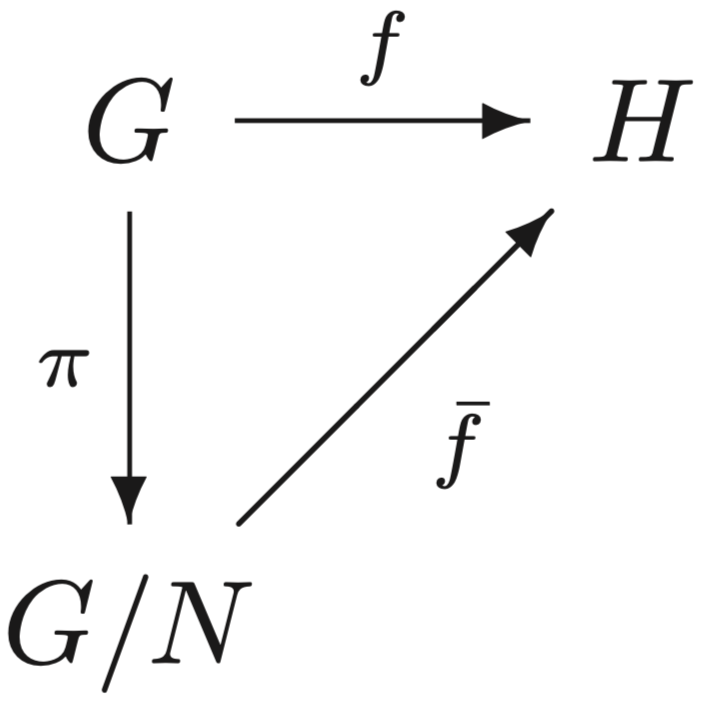
\includegraphics[width=0.2\textwidth]{Figs/2.png}
\end{figure}
\vspace{-0.55cm}
% \subsubsection{Application of Orbit-Stabiliser Theorem}

We would like to find a homomorphism $\bar{f}: G / N \rightarrow H$ that makes the diagram \tb{commute}, namely
\begin{align*}
f(a)=\bar{f}(\pi(a))
\end{align*}
for all $a \in G$
\begin{thma}\bfs{Factor Theorem}\label{thm:aondca}
Any homomorphism $f$ whose kernel $K$ contains $N$ can be factored through $G / N$. In other words, there is a \tb{unique homomorphism} $\bar{f}: G / N \rightarrow H$ such that $\bar{f} \circ \pi=f$. Furthermore
\begin{enumerate}
    \item $\bar{f}$ is an \tb{epimorphism} if and only if $f$ is.
    \item $\bar{f}$ is a \tb{monomorphism} if and only if $K=N$.
    \item $\bar{f}$ is an \tb{isomorphism} if and only if $f$ is an epimorphism and $K=N$.
\end{enumerate}
\end{thma} 
\begin{proof}
\tb{Unicity.} Let us start by proving that if there exists $\bar{f}$ such that $\bar{f} \circ \pi=f$, then it is unique. Let $\tilde{f}$ be another homomorphism such that $\tilde{f} \circ \pi=f$. We thus have that
\begin{align*}
(\bar{f} \circ \pi)(a)=(\tilde{f} \circ \pi)(a)=f(a)
\end{align*}
for all $a \in G$, that is
\begin{align*}
\bar{f}(a N)=\tilde{f}(a N)=f(a) .
\end{align*}
This tells us that for all $b N \in G / N$ for which there exists an element $b$ in $G$ such that $\pi(b)=b N$, then its image by either $\bar{f}$ or $\tilde{f}$ is determined by $f(b)$. This shows that $\bar{f}=\tilde{f}$ by \tb{surjectivity} of $\pi$.

\tb{Existence.} Let $a N \in G / N$ such that $\pi(a)=a N$ for $a \in G$. We define
\begin{align*}
\bar{f}(a N)=f(a) .
\end{align*}
This is the most natural way to do it, however, we need to make sure that this is indeed well-defined, in the sense that it should not depend on the choice of the representative taken in the coset. Let us thus take another representative, say $b \in a N$. Since $a$ and $b$ are in the same coset, they satisfy $a^{-1} b \in N \subset K$, where $K=\operatorname{Ker}(f)$ by assumption. Since $a^{-1} b \in K$, we have $f\left(a^{-1} b\right)=1$ and thus $f(a)=f(b)$.

Now that $\bar{f}$ is well defined, let us check this is indeed a group homomorphism. First note that $G / N$ is indeed a group since $N \triangleleft G$. Then, we have
\begin{align*}
\bar{f}(a N b N)=\bar{f}(a b N)=f(a b)=f(a) f(b)=\bar{f}(a N) \bar{f}(b N)
\end{align*}
and $\bar{f}$ is a homomorphism.
\begin{enumerate}
    \item The fact that $\bar{f}$ is an epimorphism if and only if $f$ is comes from the fact that both maps have the same image.
    \item First note that the statement $\bar{f}$ is a monomorphism if and only if $K=N$ makes sense since $K=\operatorname{Ker}(f)$ is indeed a normal subgroup, as proved earlier.

To show that $\bar{f}$ is a monomorphism is equivalent to show that $\operatorname{Ker}(\bar{f})$ is trivial. By definition, we have
\begin{align*}
\begin{aligned}
\operatorname{Ker}(\bar{f}) &=\{a N \in G / N, \bar{f}(a N)=1\} \\
&=\{a N \in G / N, \bar{f}(\pi(a))=f(a)=1\} \\
&=\{a N \in G / N, a \in K=\operatorname{Ker}(f)\}
\end{aligned}
\end{align*}
So the kernel of $\bar{f}$ is exactly those cosets of the form $a N$ with $a \in K$, but for the kernel to be trivial, we need it to be equal to $N$, that is we need $K=N$.
\item This is just a combination of the first two parts.
\end{enumerate}
\end{proof}

\subsection{Direct Products and Direct Sums}
\subsubsection{(External) Direct Products}
\begin{defa}{\bfs{(External) Direct Product}}
 Let $G$ and $H$ be two groups, with respective identities $e_{G}$ and $e_{H} .$ We may form the \tb{(external) direct product} $G \times H=\{(x, g) \mid x \in G, g \in H\} .$ Let $x, y \in G$ and $g, h \in H .$ Observe that there is a natural binary operation on $G \times H$ given by:
\begin{align*}
(x, g) *(y, h):=(x y, g h)
\end{align*}
\end{defa} 
\begin{lema}
$G \times H$ is a group under the natural binary operation.
\end{lema}
\begin{proof}Check the 3 conditons:
\begin{enumerate}
    \item Associativity holds for both $G$ and $H \Rightarrow$ associativity hold for $G \times H$.
    \item $\left(e_{G}, e_{H}\right)$ is the identity.
    \item  For $g \in G$ and $h \in H(g, h)^{-1}=\left(g^{-1}, h^{-1}\right)$.
\end{enumerate} 
\end{proof}
\begin{rema}
There is an obvious generalization of this concept to \tb{the product of any finite collection of groups}.
\end{rema}
\begin{thma}
Let $G$ and $H$ be finite cyclic groups. Then $G \times H$ is cyclic if and only if $|G|$ and $|H|$ are relatively prime.
\end{thma}
\begin{proof}
Let $|G|=m$ and $|H|=n$, so that $|G \times H|=m n$. To prove the first half of the theorem, we assume $G \times H$ is cyclic and show that $m$ and $n$ are relatively prime. Suppose that $\gcd(m, n)=d$ and $(g, h)$ is a generator of $G \times H$. Since $(g, h)^{m n / d}=\left(\left(g^{m}\right)^{n / d},\left(h^{n}\right)^{m / d}\right)=(e, e)$, we have $m n=|(g, h)| \leq m n / d$. Thus, $d=1$.

To prove the other half of the theorem, let $G=\langle g\rangle$ and $H=\langle h\rangle$ and suppose $\operatorname{gcd}(m, n)=1$. Then, $|(g, h)|=\operatorname{lcm}(m, n)=m n=|G \times H|$, so that $(g, h)$ is a generator of $G \times H$.
\end{proof}
\begin{cora}\bfs{Criterion for $G_{1} \times G_{2} \times \cdots \times G_{n}$ to Be Cyclic}
An external direct product $G_{1} \times G_{2} \times \cdots \times G_{n}$ of a finite number of finite cyclic groups is cyclic if and only if $\left|G_{i}\right|$ and $\left|G_{j}\right|$ are relatively prime when $i \neq j$.
\end{cora}
\begin{cora}\bfs{Criterion for $Z_{n_{1} n_{2} \cdots n_{k}} \cong Z_{n_{1}} \times Z_{n_{2}} \times \cdots \times Z_{n_{k}}$}\label{cor:odmnfafgxz}
Let $m=n_{1} n_{2} \cdots n_{k}$. Then $Z_{m}$ is isomorphic to $Z_{n_{1}} \times Z_{n_{2}} \times \cdots \times Z_{n_{k}}$ if and only if $n_{i}$ and $n_{j}$ are relatively prime when $i \neq j$.
\end{cora}
\begin{proof}
This is because cyclic of $Z_{n_{2}} \times \cdots \times Z_{n_{k}}$ and \cref{thm:cyc_twocase}.
\end{proof}
\begin{exma}
By using the results above in an iterative fashion, one can express the same group (up to isomorphism) in many different forms. For example, we have
$$
Z_{2} \times Z_{2} \times Z_{3} \times Z_{5} \cong Z_{2} \times Z_{6} \times Z_{5} \cong Z_{2} \times Z_{30}
$$
\end{exma}


\subsubsection{Direct Sum (Internal Direct Product) }
\begin{defa}{\bfs{Direct Sum}}\label{def:dir_sum}
 Let $G$ be a group and $H, K \subset G$ two \tb{subgroups}. Let us furthermore assume that
\begin{enumerate}
    \item $\forall h \in H$ and $\forall k \in K, h k=k h .$
    \item Given $g \in G$ there exist \tb{unique} $h \in H, k \in K$ such that $g=h k$.
\end{enumerate}
Under these circumstances we say that $G$ is the direct sum of $H$ and $K$ and we write $G=H \oplus K$. 
\end{defa} 
\begin{rema}{\bfs{equivalent condition and explanation}}We explain these two conditions:
\begin{enumerate}
    \item     The first condition is similar to Abelian, however we only require this \tb{commutative} over $H$ and $K$. Note in some books \cite{gallian2021contemporary}[Page 183], they use definition with $H$ and $K$ to be normal groups. This is \tb{more strict} as this definition implies our definition \cite{gallian2021contemporary}[Theorem 9.6].
    \item The second property guarantee uniqueness of the decomposition (see \cite[page 2]{horn2012matrix}) and it is equivalent to:
\begin{itemize}
    \item  $H \cap K=\left\{e_{G}\right\}$ and for $g \in G$ there exist $h \in H, k \in K$ such that $g=h k$. 
\end{itemize}
From the second property, we can define  \cref{eq:doncadf}. It may be confused why for every $h$ and $k$, we can define the map $hk\in G$. This is because $H$ and $K$ are all subgroups of $G$ so the operation is closed. So the second property should be read as:
\begin{itemize}
    \item   \cref{eq:doncadf} is a bijection.
\end{itemize}
\item The generalization of this concept to the direct sum of any finite collection of groups can be seen at \cite{gallian2021contemporary}[Page 184].
\end{enumerate}

\end{rema}
\begin{rema}{\bfs{thinking}}\label{rem:dfgv}
 What's the  fundamental reason of ``$f$ injective if and only if $\Ker(f)=\{e_G\}$ in  \cref{lem:hom_bi_e} `` and  $H \cap K=\left\{e_{G}\right\}$  guarantee uniqueness''?
    \begin{enumerate}
        \item[$\bullet$] \tb{The general answer is (linear) tensor over groups}.  \cref{lem:hom_bi_e}  is the special case of $1$-tensor, while the above direct sum is $2$-tensor over the product $H\times K$. If the kernel of the homomorphism \cref{eq:doncadf} is $\{(e_G,e_G)\}$. We know it is injective. $\{(e_{G},e_{G})\}$ just means $H \cap K=\left\{e_{G}\right\}$ (hint: $H \cap K$ is a group, if $H \cap K\ne \left\{e_{G}\right\}$, we will get that  the kernel is not $\{(e_{G},e_{G})\}$).
    \end{enumerate}
\end{rema}
\begin{exma}
For example, $(\mathbb{Z} / 15 \mathbb{Z},+)$ is the direct sum of $\gp([3])$ and $\gp([5])$
\end{exma}

\begin{thma}{\bfs{direct sum isomorphic to direct product}}
 If $G$ is the direct sum of the subgroups $H, K \subset G$ then:
 $$H \oplus K \cong H \times K$$
\end{thma}
\begin{rema}
The concept of direct sum has a clear generalization to any finite collection of subsets of $G$.
\end{rema}
\begin{proof}
Define the map
\begin{align}
\begin{aligned}\label{eq:doncadf}
\phi: H \times K & \rightarrow G \\
(h, k) & \mapsto h k
\end{aligned}
\end{align}
Let $x, y \in H$ and $g, h \in K .$ By property 1, we have $\phi((x, g)*(y, h))=\phi(x y, g h)=x y g h=x g y h=$ $\phi(x, g) \phi(y, h) .$ Hence $\phi$ is a homomorphism. Property two ensures that $\phi$ is bijective.% as shown in \cref{rem:dfgv}.
\end{proof} 
\begin{cora}
If normal groups $H\cap K=\{e\}$ and are subgroups of $G$, we have  $H \oplus K \cong H \times K$ which may not surjective over $G$. But note according to \cref{eq:doncadf}, $H \oplus K$ must be a group as the image of the map \cref{eq:doncadf}.
\end{cora}
\subsubsection{Relation to Chinese Reminder Theorem, Unit Group}
$\bullet$ Notation Clarify:
\begin{enumerate}
    \item For notation simplicity, in this section, we denote $\mathbb{Z}/ {n}\mathbb{Z}$ as $\mathbb{Z}_{n}$.  
    \item Let \tb{unit group} $\mathbb{U}_{n} \subseteq \mathbb{Z}_{n}$ consist of those $[u]$ such that for some $[v],[u] \cdot[v]=[1]$, namely, those elements of $\mathbb{Z}_{n}$ that have multiplicative inverses. Note the group operation now is \tb{multiplication} of modulo.
\end{enumerate}
We first recall Chinese Remainder Theorem and its corollary:
\begin{thma}\bfs{Chinese Remainder Theorem}\label{thmn:chinese}
Suppose $n=a b$, with $a$ and $b$ relatively prime. For $x=0,1, \ldots, n-1$, associate $[x] \in \mathbb{Z}_{n}$ with $([x],[x]) \in \mathbb{Z}_{a} \times \mathbb{Z}_{b}$ (note that the symbol $[x]$ means different things in $\mathbb{Z}_{n}, \mathbb{Z}_{a}$ and $\left.\mathbb{Z}_{b}\right)$. This gives a \tb{one-to-one} correspondence between $\mathbb{Z}_{n}$ and $\mathbb{Z}_{a} \times \mathbb{Z}_{b}$.
\end{thma} 
\begin{cora}\label{cor:onkenq}
Suppose $n=a b$, with $a$ and $b$ relatively prime. For $x=$ $0,1, \ldots, n-1$, if $[x] \in \mathbb{U}_{n}$, associate $[x]$ with $([x],[x]) \in \mathbb{Z}_{a} \times \mathbb{Z}_{b}$. This gives a \tb{one-to-one} correspondence between $\mathbb{U}_{n}$ and $\mathbb{U}_{a} \times \mathbb{U}_{b}$.
\end{cora}


$\bullet$ \tb{But note $\mathbb{Z}_{a}$ and $\mathbb{Z}_{b}$ do not satisfy the conditions of intersection is $\{[0]\}$. What is happening?}
\begin{enumerate}
    \item \cref{cor:odmnfafgxz} is the group version (isomorphic, more than bijiection) of Chinese Remainder Theorem \cref{thmn:chinese}. Note in \cref{cor:odmnfafgxz}, cyclic is the key. We does not care the direct sum here.
        \item $\gp{[a]}\cap \gp{[b]}=\{[0]\}$  if $a$ and $b$ are coprime is clear since otherwise it mean $\LCM(a,b)<ab$. 
    \item But what's the relation between $\bbZ_{ab}\cong\mathbb{Z}_{a} \times \mathbb{Z}_{b}\cong \gp{[a]}\times \gp{[b]} \cong \gp{[a]}\oplus \gp{[b]}=\bbZ_{ab}$, where ${[a]}$ is in terms of $\bmod ab$?
    
    \tb{Key:} this is the trick of multiple each element in $\mathbb{Z}_{a}$ by $b$, and you will get $\gp{[b]}$; or we note $\gp{[b]}$ is a cyclic group with order $b$, so it must isomorphic to $\bbZ_b$.
    \item Similary, we can also get $\bbU_{ab} \cong \bbU_a \times \bbU_b \cong \bbU_{ab}^{(a)} \times \bbU_{ab}^{(b)} \cong \bbU_{ab}^{(a)} \oplus \bbU_{ab}^{(b)}$;

\end{enumerate}

We next list the facts that have been stated in number theory notes or in \cite{gallian2021contemporary}:
\begin{enumerate}
    \item \begin{defa}
Suppose that $n=de$. Let $G_{e}=\{x: 0 \leq x<n$ and $(x, n)=e\}$, that is, $G_{e}$ consists of all numbers whose gcd with $n$ is $e$.
\end{defa}
\item \begin{defa}
$$
R_{d}=\{y: 0 \leq y<d \text { and }(y, d)=1\}
$$
Notice that this definition makes sense even for $d=1$, namely, $R_{1}=\{0\}$, and in every case, the number of elements in $R_{d}$ is $\phi(d)$ (because $R_{d}$ is almost $\mathbb{U}_{d}$, missing the $[\cdot]$ again). 
\end{defa}
\item \begin{defa}
 If $k$ is a divisor of $n$, let
$$
\bbU_{n}^{(k)}=\{x \in \bbU_n \mid x \bmod k=1\}
$$
This is a group. I skim the proof here.
\end{defa}
\end{enumerate}

\begin{lema}
From  number theory notes, we have $|G_e|=|R_d|$ according to 
\begin{align}
    (y, d)=1 \quad \text { iff } \quad(e y, e d)=e \quad \text { iff } \quad(e y, n)=e\label{eq:qijnnd}
\end{align}
\end{lema}
\begin{rema}
Note here is a general conclusion, no need $d$ and $e$ are coprime. But below we need \tb{coprime} condition.
\end{rema}

\begin{lema}\label{lem:zundf}
Suppose $a$ and $b$ are relatively prime. Then $\bbU_{ab}$ is isomorphic to the external direct product of $\bbU_a$ and $\bbU_b$. We have
\begin{enumerate}
    \item $\bbU_{ab} \cong \bbU_a \times \bbU_b$;
    \item $\bbU_{ab}^{(a)}\cong\bbU_b$;
    \item $\bbU_{ab}^{(b)}\cong\bbU_a$.
\end{enumerate}
\end{lema}
\begin{proof}We can construct the following.
\begin{enumerate}
    \item An isomorphism from $\bbU_{ab}$ to $\bbU_a \times \bbU_b$ is $x \rightarrow(x \bmod a, x \bmod b)$;
    \item An isomorphism from $\bbU_{ab}^{(a)}$ to $\bbU_b$ is $x \rightarrow x \bmod b$;
    \item  An isomorphism from $\bbU_{ab}^{(b)}$ to $\bbU_a$ is $x \rightarrow x \bmod a$. 
\end{enumerate}
\end{proof}
\begin{rema}
The first is obvious the isomorphic group version of \cref{cor:onkenq}. But what's the second and third means? It becomes obvious if we note the similar trick of \cref{eq:qijnnd}: it is just a factor trick. 
\end{rema}
\begin{lema}
If $a$ and $b$ are relatively prime positive integers then $\bbU_{ab}=\bbU_{ab}^{(a)} \oplus \bbU_{ab}^{(b)} \cong\bbU_{ab}^{(a)} \times \bbU_{ab}^{(b)}$.
\end{lema}
\begin{proof}
Here, we only need to show $\bbU_{ab}^{(a)} \cap \bbU_{ab}^{(b)}=\{[1]\}$.  If otherwise $[1]\ne [w] \in \bbU_{ab}^{(a)} \cap \bbU_{ab}^{(b)}$. We have $w\equiv 1\bmod a$ and $w \equiv 1\bmod b$. But this just means $a$ and $b$ are not coprime (think carefully here), a contradiction. We therefore have the conclusion $\bbU_{ab}^{(a)} \times \bbU_{ab}^{(b)}\cong \bbU_{ab}^{(a)} \oplus \bbU_{ab}^{(b)}$ according to \cref{eq:doncadf} and $\bbU_{ab}\cong \bbU_{ab}^{(a)}\times \bbU_{ab}^{(a)}$ according to \cref{lem:zundf}. From the finite size, we then have the map \cref{eq:doncadf} is surjective on $\bbU_{ab}$ and hence get "$=$".
\end{proof}
% \begin{rema}
%  Note the one-to-one correspondence the \tb{generalization} of the one in the Direct Sum and Direct Sum in Algebra note.
% \end{rema}

\subsection{Finitely Generated Abelian Groups}\label{sec:cxvdf}
Let $G$ be an \tb{Abelian group}. We shall now use additive '$+$' notation to express composition within $G$. In particular we will denote the identity by $0$ (not to be confused with $0 \in \mathbb{Z})$. We do this because we are very familiar with addition on $\mathbb{Z}$ being commutative. 

Given $m \in \mathbb{Z}$ and $a \in G$, we write
\begin{align*}
m a= \begin{cases}a + a + \cdots + a(m \text { times }), & \text { if } m>0 \\ 0, & \text { if } m=0 \\ a^{-1} + a^{-1} + \cdots + a^{-1}(-m \text { times }), & \text { if } m<0\end{cases}
\end{align*}
\begin{lema}\label{lem:abe_pro}
 Use Abelian properties, we have that $\forall a, b \in G ; m, n \in \mathbb{Z}$ :
\begin{enumerate}
    \item $m(a+b)=m a+m b$
    \item $(m+n) a=m a+n a$
    \item $(m n) a=m(n a)$
\end{enumerate}
\end{lema}
\begin{rema}
Note here $ma$ is not the multiplication of two elements in $G$, it is one integer and one element in $G$. Compare also with \cref{lem:odnndsaff}.
\end{rema}

From now in this section we assume that

\centerline{\tb{$G$ is \tb{finitely generated Abelian group}}}

\begin{defa}{\bfs{Basis}}
$\exists\left\{a_{1}, \cdots, a_{n}\right\} \subset G$ such that $
\gp\left(\left\{a_{1}, \cdots, a_{n}\right\}\right)=$
$G$. In other words, because $G$ is Abelian, every $x \in G$ can be written in the form
\begin{align}
x=\lambda_{1} a_{1}+\cdots+\lambda_{n} a_{n} \quad \lambda_{i} \in \mathbb{Z} \label{eq:dec_bas}
\end{align}

If every expression of the above form was \tb{unique} (\tb{after possibly restricting $0\leq \lambda_{1}<\operatorname{ord}(a_{i})$}) for a given $x \in G$.  We call $\left\{a_{1}, \cdots, a_{n}\right\}$ a \tb{basis} for $G$.
\end{defa}

\begin{rema}
In general such the expression in \cref{eq:dec_bas} is \tb{not unique.} For example is $G$ is of order $m \in \mathbb{N}$ then $(m+1) a=a$ for all $a \in G$. This is because $m a=0$.
Observe that it is not clear that such a basis even exists at present.
\end{rema}
\begin{lema}{\bfs{Direct Sum Decomposition}}
If $\left\{a_{1}, \cdots, a_{n}\right\} \subset G$ were a basis then letting $A_{i}=\gp\left(a_{i}\right) \subset G$ we have the direct sum decomposition:
\begin{align*}
G=A_{1} \oplus \cdots \oplus A_{n}
\end{align*}
Conversely, if $\mathrm{G}$ can be represented as the direct sum of cyclic subgroups then choosing a generator for each gives a basis for $G$.
\end{lema}
 \begin{proof}
% \begin{align}
%     \text{``unique''} \Leftrightarrow \gp(\{a_{i}\}) \cap \gp(\{a_{j}\})=\{0\}\text{ for all } i\ne j. \label{eq:uni_0}
% \end{align}
Since $G$ is Abelian, from \cref{def:dir_sum}, we know that the two direction are both correct in the lemma.
 \end{proof}
 \subsubsection{Torsion, Torsion Free, Free Abelian}
\begin{defa}{\bfs{Torsion, Torsion Subgroup: finite order}}
Let $G$ be an Abelian group. $x \in G$ is \tb{torsion} is it is of finite order. We denote the subgroup of torsion elements by $tG \subset G$, called the \tb{torsion subgroup.}
\end{defa} 
\begin{lema}
 $tG \subset G$ is indeed a subgroup.
\end{lema}
\begin{proof}
This critically requires that $G$ be Abelian from properties list in \cref{lem:abe_pro}. It is not true in general.
\begin{enumerate}
    \item $\operatorname{ord}(0)=1 \Rightarrow 0 \in t G$
    \item  Let $g, h \in t G \Rightarrow \exists n, m \in \mathbb{N}$ such that $n g=m g=0 \Rightarrow n m(g+h)=(m n g+n m h)=$
$m 0+n 0=0 \Rightarrow g+h \in t G$
\item $n g=0 \Rightarrow-(n g)=n(-g)=0$. Hence $g \in t G \Rightarrow-g \in t G$
\end{enumerate}
\end{proof} 

\begin{defa}{\bfs{Torsion Group vs. Torsion Free Group}}
 If $tG=G$ we say that $G$ is a \tb{torsion group}. If $tG=\{0\}$ we say that $G$ is \tb{torsion free}.
\end{defa}
\begin{lema}
 If $G$ is torsion and finitely generated then $G$ is finite.
\end{lema} 
\begin{rema} Under condition finitely generated G, we have 

\centerline{\tb{$G$ is finite $\Leftrightarrow$ $tG=G$.}}
\end{rema}
\begin{proof}
Let $\left\{a_{1}, \cdots, a_{n}\right\} \subset G$ be a generating set. Each element is of finite order hence every element $x \in G$ can be written in the form
\begin{align*}
x=\lambda_{1} a_{1}+\cdots+\lambda_{n} a_{n}, \quad \lambda_{i} \in \mathbb{Z}, 0 \leq \lambda_{1}<\operatorname{ord}\left(a_{i}\right)
\end{align*}
This is a finite set.
\end{proof} 
\begin{lema}
 $G/tG$ is a torsion free Abelian group.
\end{lema} 
\begin{proof}
Firstly note that $t G \subset G$ is normal as $G$ is Abelian, hence $G / t G$ is naturally an abelian group. Let $x \in G$. Assume that $x+t G \in G / t G$ is torsion. Hence $\exists n \in \mathbb{N}$ such that $n(x+t G)=n x+t G=t G$ (last equality is from $x+t G$ is torsion). Hence $n x \in t G$ so $\exists m \in \mathbb{N}$ such that $m n x=0$. Hence $x \in t G \Rightarrow x+tG=t G$.
\end{proof} 
\begin{rema}
Here we use notation  $x+t G$. This is the same as $xtG$ but we include $+$ for better understanding.
\end{rema}
\begin{defa}{\bfs{Free Abelian}}
 An finitely generated Abelian group $G$ is said to be \tb{free Abelian} if there exists a finite generating set $\left\{a_{1}, \cdots, a_{n}\right\} \subset G$ such that every element of $G$ can be \tb{uniquely} expressed as
\begin{align*}
\lambda_{1} a_{1}+\cdots \lambda_{n} a_{n} \text { where } \lambda_{i} \in \mathbb{Z}
\end{align*}
In other words, if we can find a basis for $G$ consisting of \tb{non-torsion} elements.
\end{defa} 
\begin{rema}{\bfs{explanation}}
\begin{itemize}
    \item {Non-torsion} is from $\lambda_{i} \in \mathbb{Z}$. Compare also with \cref{eq:dec_bas} where the uniqueness may be there  in the sense of  \tb{after possibly restricting $0\leq \lambda_{1}<\operatorname{ord}(a_{i})$}.
    \begin{itemize}
        \item[$\ast$] $\gp(\{a_i\})$ is infinite for each $i$.
    \end{itemize}
    \item We still have 
    \begin{align}
   \hspace{-1cm} ``\sum \lambda_i a_i=0 \Rightarrow \lambda_{i}=0 \text{ for all } i " \Leftrightarrow \text{``unique''} \Leftrightarrow \gp(\{a_{i}\}) \cap \gp(\{a_{j}\})=\{0\}\text{ for all } i\ne j. \label{eq:uni_1}
\end{align}
\end{itemize}
 
\end{rema}




In this case
\begin{align}
G=\gp\left(a_{1}\right) \oplus \cdots \oplus \gp\left(a_{n}\right) \cong \mathbb{Z} \times \mathbb{Z} \cdots \times \mathbb{Z}=\mathbb{Z}^{n}\label{eq:free_abe_Zn}
\end{align}
\begin{lema}
 Let $G$ be a finitely generated \tb{free abelian} group. Any two bases must have the same cardinality.
\end{lema} 
\begin{proof}
 Let $\left\{a_{1}, \cdots, a_{n}\right\} \subset G$ be a basis. Let $2 G:=\{2 x \mid x \in G\}$. $2 G \subseteq G$ is a subgroup. Observe that $2 G=\left\{\lambda_{1} a_{1}+\cdots \lambda_{n} a_{n} \mid \lambda_i \in 2 \mathbb{Z}\right\} .$ Hence $(G: 2 G)=2^{n} .$ But the left hand side is defined independently of the basis, so $2^n$ (and hence $n$) is independently of the basis. The result follows.
\end{proof}

\begin{defa}{\bfs{Rank}}
 Let $G$ be a finitely generated free Abelian group. The rank of $G$ is the size of any basis.
\end{defa} 
\begin{thma}
A finitely generated abelian group is free Abelian $\Longleftrightarrow$ it is torsion free.
\end{thma} 
\begin{proof}
 $(\Rightarrow)$ is trivial. Assume not torsion free but free Abelian, we have a basis $\{a_1,...,a_n\}$. $\exists x=\sum_i \lambda_i a_i\ne 0$ and $mx=x,m>1$, then $\sum (\lambda_im-\lambda_i)a_i=0$ which is impossible from \cref{eq:uni_1}, a contradiction.
 
$(\Leftarrow)$
Assume $G$ is torsion-free, let $\left\{a_{1}, \cdots, a_{n}\right\} \subset G$ generate $G .$ We will prove the result by induction on $n$. 

Base Case: $n=1, G=\gp(a) \cong(\mathbb{Z},+)$ from \cref{thm:cyc_twocase}, which is free abelian. Therefore result is true for $n=1$.

If $\left\{a_{1}, \cdots, a_{n}\right\} \subset G$ is a basis we have nothing to prove since now basis guarantees unique (after possbile restricting to $0$ to $\ord(a_i)$), the torch free then further guarantees $\ord(a_i)$ is not finite, and we get \cref{eq:free_abe_Zn}.
Suppose that it is not a basis. then we have a non-trivial relation:
\begin{align*}
\lambda_{1} a_{1}+\lambda_{2} a_{2}+\cdots+\lambda_{n} a_{n}=0
\end{align*}
If $\exists d \in \mathbb{Z}$ such that $d \mid \lambda_{i}$ for all $i$, then have $d\left(\frac{\lambda_{1} a_{1}}{d}+\frac{\lambda_{2} a_{2}}{d}+\cdots+\ldots\right)=0 .$ As $G$ is torsion-free, $\left(\frac{\lambda_{1} a_{1}}{d}+\frac{\lambda_{2} a_{2}}{d}+\cdots+\ldots\right)=0 .$ We can therefore \tb{assume that the $\lambda_{i}$ are collectively coprime.} 

1). If exist a coefficient $=1$, wlog, $\lambda_{1}=1$, then we can shift terms to get $a_{1}=-\left(\lambda_{2} a_{2}+\lambda_{3} a_{3}+\cdots+\lambda_{n} a_{n}\right) .$ Therefore, $G$ is generated by the $\left\{a_{2}, \cdots, a_{n}\right\} \subset G$ and the result follows by induction from the $n-1$ case. \\
2). Otherwise, we will reduce to the above case as use the following additional steps: Assume all $\lambda_i\ge 2$ (cannot $\ne 1$; if $\lambda_i=0$, just remove $a_i$). Assume $\left|\lambda_{1}\right| \geq\left|\lambda_{2}\right|>0 .$ By the remainder theorem we may choose $\alpha \in \mathbb{Z}$ such that $\left|\lambda_{1}-\alpha \lambda_{2}\right|<\left|\lambda_{2}\right| .$ Let $a_{2}^{\prime}=a_{2}+\alpha a_{1}$ and $\lambda_{1}^{\prime}=\lambda_{1}-\alpha \lambda_{2}$, then
\begin{align*}
\lambda_{1}^{\prime} a_{1}+\lambda_{2} a_{2}^{\prime}+\cdots+\lambda_{n} a_{n}=0
\end{align*}
Also observe that $\left\{a_{1}, a_{2}^{\prime}, \cdots, a_{n}\right\} \subset G$ is still a generating set and $\left\{\lambda_{1}^{\prime}, \cdots, \lambda_{n}\right\}$ are still collectively coprime. This process must must eventually terminate (because of coprime) with one of the coefficients equal either 1 or $-1 .$ In this case we can apply the inductive step as above to conclude that $G$ is free abelian. 
\end{proof}
\begin{thma}
Let $G$ be finitely generated and Abelian. Then $G / t G$ is a finitely generated free Abelian group.
\end{thma} 

\begin{proof}
 $G / t G$ is torsion free. We must show that $G / t G$ is finitely generated. Let $\left\{a_{1}, \cdots, a_{n}\right\} \subset$ $G$ generate $G$. Then $\left\{a_{1}+t G, \cdots, a_{n}+t G\right\} \subset G / t G$ forms a generating set. By the above theorem $G / t G$ is free Abelian. 
\end{proof}

\begin{defa}{\bfs{Rank: finitely generated Abelian group}}
 Let $G$ be a finitely generated Abelian group. We define the rank of $G$ to be the rank of $G / t G$
\end{defa} 
\subsubsection{Decomposition of Finitely Generated Abelian Group}
Let $G$ be finitely generated and Abelian with  $G / t G$ being the free Abelian group with rank $n$. We can select $\{f_{1}, \cdots, f_{n}\}$ as a basis for $G / t G$, where $f_{i}$ of course has infinite order.

Let $\phi: G \rightarrow G / t G$ be the natural quotient homomorphism (\cref{thm:xxh}) which is surjective of course:
\begin{align*}
    \phi: G &\rightarrow G / t G \\
    x &\mapsto x+tG
\end{align*}

Choose $\left\{e_{1}, \cdots, e_{n}\right\} \subset G$ such that $\phi\left(e_{i}\right)=f_{i}, \forall i \in\{1, \cdots, n\} .$ Since none of the $f_{i}$ have finite order, we get that none of the $e_{i}$ have finite order. Moreover, from homomorphism we have that
\begin{align*}
\phi\left(\lambda_{1} e_{1}+\cdots+\lambda_{n} e_{n}\right)=\lambda_{1} f_{1}+\cdots+\lambda_{n} f_{n} \in G / t G
\end{align*}
Then, we have $\lambda_{1} e_{1}+\cdots+\lambda_{n} e_{n}=0 \Longleftrightarrow$
$\lambda_{i}=0, \forall i$. We define
$$F:=\gp\left\{e_{1}, \cdots, e_{n}\right\} \subseteq G$$
which is is free abelian with basis $\left\{e_{1}, \cdots, e_{n}\right\}$, so \tb{$F$ is torsion
free}. Therefore $F \cap t G=\{0\}$. 

Let $g \in G$. By definition, $\exists \lambda_{1}, \cdots, \lambda_{n} \in \mathbb{Z}$ such that $\phi(g)=\lambda_{1} f_{1}+\cdots+\lambda_{n} f_{n}$. Then we
have:
\begin{align*}
\begin{aligned}
\phi(g)=\lambda_{1} f_{1}+\cdots+\lambda_{n} f_{n} & \Rightarrow \phi(g)=\phi\left(\lambda_{1} e_{1}+\cdots+\lambda_{n} e_{n}\right) \\
& \Rightarrow \phi\left(g-\left(\lambda_{1} e_{1}+\cdots+\lambda_{n} e_{n}\right)\right)=0 \\
& \Rightarrow g-\left(\lambda_{1} e_{1}+\cdots+\lambda_{n} e_{n}\right) \in \Ker \phi=t G \\
& \Rightarrow \exists h \in t G \text { s.t. } g=\left(\lambda_{1} e_{1}+\cdots+\lambda_{n} e_{n}\right)+h
\end{aligned}
\end{align*}
\centerline{\tb{Hence every $x$ may be written uniquely in the form $x=f+g$ where $f \in F$ and $g \in t G$}}
\begin{thma}{\bfs{Decomposition Theorem}}
Every finitely generated Abelian group can be written as a direct sum of a free Abelian group and a \tb{finite} group.
\end{thma} 
\begin{proof}
By the above, we may write
\begin{align*}
G=F \oplus t G
\end{align*}
$F$ is free Abelian by construction. We next prove $tG$ is finite. Define the homomorphism :
\begin{align*}
\begin{aligned}
G=F \oplus t G & \rightarrow t G \\
f+h & \mapsto h
\end{aligned}
\end{align*}
This is surjective with kernel $F$, hence by the first isomorphism theorem $t G$ is isomorphic to $G / F$. The image of any generating set of $G$ is a generating set for $G / F$ under the quotient homomorphism. Hence $t G$ is \tb{finitely generated} and torsion, hence finite. 
\end{proof} 

Hence we have reduced the study of finitely generated Abelian groups to understanding finite Abelian groups:
\begin{align}
G\cong \mathbb{Z}^{n}\oplus tG
\end{align}
where $tG$ is finite. See also \cref{eq:free_abe_Zn}.


\subsection{Finite Abelian Groups}
\begin{defa}{\bfs{$p$-group}}
 A finite group $G$ (not necessarily Abelian) is a $p$-group, with $p \in \mathbb{N}$, a prime, if every element of $G$ has order a power of $p$.
\end{defa} 
\begin{lema}\label{lem:djfdacf}
 The order of a finite $p$-group must be a power of $p$.
\end{lema}
\begin{proof}
We prove by contradiction. Assume $|G|=p^nu_1\ldots u_n$, where $\HCF(p,u_i)=1$ for all $i$.  By Sylow's Theorem \cref{thm:sylow}, we have that there exist a subgroup $M$ of $G$ with size $u_i$. Let $x\in M$ but $x\ne e_G$. We then have $\gp(x)$, a subgroup of $M$. But note $x$ need to be a power of $p$ according to the definition of  $p$-group. So we have $p|u_i$ which is impossible.
\end{proof}
From now in this section we assume that

\centerline{\tb{$G$ is \tb{finite Abelian group}}}

Let $p \in \mathbb{N}$ be a prime. We define $G_{p}:=\{g \in$ $G \mid$ ord $(p)$ is a power of $p\} \subset G$
\begin{thma}
$G_{p} \subset G$ is a subgroup.
\end{thma}
\begin{proof}
\begin{enumerate}
    \item  $\operatorname{ord}(0)=1=p^{0} \Rightarrow 0 \in G_{p}$
    \item Let $g, h \in G_{p} \Rightarrow \exists r, s \in \mathbb{N}$ such that $p^{r} g=p^{s} h=0 \Rightarrow p^{r+s}(g+h)=p^{s}\left(p^{r} g\right)+p^{r}\left(p^{s} h\right)=$
$0+0=0 \Rightarrow g+h \in G_{p}$
\item Let $g \in G_{p} \Rightarrow \exists r \in \mathbb{N}$ such that $p^{r} g=0 \Rightarrow-p^{r} g=p^{r}(-g)=0 \Rightarrow-g \in G_{p}$.
\end{enumerate}
\end{proof}
\begin{rema}
Note the above critically relies on $G$ being Abelian. 
\end{rema}

\begin{lema}We have the following facts:
 \begin{enumerate}
    \item By definition $G_{p}$ is a \tb{maximal $p$-group} contained in $G$.
     \item  $G_{p}=\{0\}$ or $p$ divides $|G|$. 
     \item By Sylow's Theorem \cref{thm:sylow}, we deduce that if $|G|=p^{n} u$, where $\HCF(p, u)=1$, then $\left|G_{p}\right|=p^{n}$. (Note, from \cref{lem:djfdacf}, we already know it has order $p^r$ with $r\le n$. Now, we further know $r=n$. Again, confirm it is the \tb{maximal}  $p$-subgroup)
 \end{enumerate}
\end{lema}  
\begin{proof}
1). By definition.

2). Two ways: one is from \cref{lem:djfdacf} directly. The other is from that if $x\in G_p$ but $x\ne 0$, then we have $\gp(x)$ will divides  $G$. Note $\ord(x)$ is a positive power of $p$. So $p\mid |G|$. Recall that $\forall g \in G$, $\operatorname{ord}(g)\mid | G |$ by Lagrange's Theorem. 

3). If  $|G_p|=p^{r}$ where $r<n$, we have $|G/G_p|=p^{n-r}u$. By Sylow's Theorem \cref{thm:sylow}, we then can select a subgroup $M$ of $G/G_p$ s.t. $|M|=p$.  We then have $G_p\subseteq H_M$ by the Third Isomorphism Theorem \cref{thm:thirdiso}. Note $|H_M|=p^{r+1}$ . We select one $x\in H_M\backslash G_p$, then we have $\ord(x)|p^{r+1}$. But this just means $x\in G_p$, a contradiction.
\end{proof}

The importance of the maximal $p$-subgroups is the following theorem.
\begin{thma}
Let $G$ is a finite Abelian group. Let $\left\{p_{1}, \cdots, p_{r}\right\}$ be the primes dividing $|G|$. Then
\begin{align*}
G=G_{p_{1}} \oplus \cdots \oplus G_{p_{r}}
\end{align*}
Moreover this is the \tb{unique} way to express as the direct sum of $p$-subgroups for distinct primes.
\end{thma}
\begin{proof}
 Let $|G|=n=a_{1} a_{2} \cdots a_{r}$ where $a_{i}=p_{i}^{\alpha_{i}} .$ Let $P_{i}=n / a_{i} .\left\{P_{1}, \cdots, P_{r}\right\} \subset \mathbb{Z}$ are
collectively coprime $\Rightarrow \exists Q_{1}, \cdots, Q_{r} \in \mathbb{Z}$ such that from \cref{cora:doncadf} we have
\begin{align*}
P_{1} Q_{1}+\cdots+P_{r} Q_{r}=1
\end{align*}
Let $g \in G$ and $g_{i}=P_{i} Q_{i} g .$ Clearly $g=g_{1}+g_{2}+\cdots+g_{r}$ and $p_{i}^{\alpha_{i}} g_{i}=Q_{i}(n g)=0$. Hence $g_{i} \in G_{p_{i}}$

We must prove the uniqueness of this sum. Assume we had
\begin{align}
g=g_{1}^{\prime}+\cdots+g_{r}^{\prime}, \quad g_{i}^{\prime} \in G_{p_{i}}\label{eq:omndnla}
\end{align}
Therefore $x=g_{1}-g_{1}^{\prime}=\left(g_{2}^{\prime}-g_{2}\right)+\left(g_{3}^{\prime}-g_{3}\right)+\cdots+\left(g_{r}^{\prime}-g_{r}\right)$. The right hand size has order dividing $P_{1}$. This is because each $g_{i}^{\prime}-g_{i}^{\prime}$, $i\ge 2$, belongs to $G_{p_i}$ which means that the order of $g_{i}^{\prime}-g_{i}^{\prime}$ is a power of $p_i$. We then have $P_1\times$right hand size$=0$. Similarly, the left hand side has order dividing $P_{i}$, $i\ge 2$. That means all $P_ix=0$, $i=1,...,r$.

Now, from the above discussion, we then have $x=\sum_{i=1}^{n} Q_iP_ix=0 \Rightarrow g_{1}=g_{1}^{\prime}$. Similarly we find
$g_{i}=g_{i}^{\prime}$ for all $i \in\{1, \cdots, r\}$, hence the sum is unique and we deduce that 
\begin{align*}
G=G_{p_{1}} \oplus \cdots \oplus G_{p_{r}}
\end{align*}
Let $\left\{q_{1}, \cdots, q_{s}\right\}$ be a finite collection of distinct primes. Assume that $G$ can be expressed as the direct sum
\begin{align*}
G=H_{1} \oplus \cdots \oplus H_{s} \cong H_{1} \times \cdots \times H_{s}
\end{align*}
where $H_{i}$ is a finite $q_{i}$-subgroup. From the The Fundamental Theorem of Arithmetic \cref{thm:fta}, clearly $\left\{p_{1}, \cdots, p_{r}\right\}=\left\{q_{1}, \cdots, q_{s}\right\}$ and any such representation is unique.
\end{proof}

\tb{$\bullet$  We have however reduced the study of finite Abelian groups to finite Abelian $p$-groups.}


\begin{thma}
Every finite Abelian $p$-group is a direct sum of cyclic groups.
\end{thma}
\begin{proof}
Let $G$ be a finite Abelian $p$-group. If $G$ is cyclic, we are done, otherwise take a cyclic subgroup $B=\gp(b)$ of \tb{maximal order}, say $p^{n}$.

\tb{Strategy:} show that there is a $p$-subgroup $D \subset G$ such that $G=B \oplus D .$ Because then we can apply this recursively to  $D$ get conclusion.

We apply the following \tb{inductive hypothesis}: For any finite Abelian $p$-group $F$ of size less than $|G|$, if $M \subset F$ is a \tb{maximal cyclic subgroup} then there exists $N \subset F$ such that $M \oplus N=F$. This is clearly true for $F$ trivial.

We claim that \tb{there is a subgroup $C$ of order $p$ such that $B \cap C=\{0\}$}: 

Recall that because $G$ is Abelian $G / B$ is naturally an Abelian $p$-group. Let $c \in G \backslash B$ and suppose $c B \in G / B$ has order $p^{r}$ for $r>0$. Observe that the maximal order of any element in $G / B$ is less than or equal to $p^{n}$ because $p^nc=0$ (recall \tb{maximal order} is $n$ for any element in $G$).

Thus we know $n \geq r$. By definition $p^{r}(c B)=B \Rightarrow p^{r} c \in B$. Thus there exists $s \in \mathbb{N}$ such that $p^{r} c=s b .$ By maximality of the order of $b$ we know $0=p^{n} c=s p^{n-r} b$. But ord $(b)=p^{n}$, hence $p^{n} \mid s p^{n-r} .$ Therefore we have $p \mid s$, say $s=p s^{\prime} .$ Hence $c_{1}=p^{r-1} c-s^{\prime} b$ has order $p$ and is not in $B$. Therefore $C=\gp\left(c_{1}\right)$ is the required subgroup.


Let $B C=\{a b \mid a \in B, b \in C\} .$ We claim that $B C \subset G$ is a subgroup.
\begin{enumerate}
    \item $e_{G} \in B$ and $e_{G} \in C \Rightarrow e_{G} \in B C$.
    \item Let $a_{1}, a_{2} \in B, b_{1}, b_{2} \in C .$ Then $\left(a_{1} b_{1}\right)\left(a_{2} b_{2}\right)=\left(a_{1} a_{2}\right)\left(b_{1} b_{2}\right) \in B C .$ Hence $B C$ is closed
under composition.
\item Let $a_{1} \in B, b_{1} \in C .$ Then $\left(a_{1} b_{1}\right)^{-1}=b_{1}^{-1} a_{1}^{-1}=a_{1}^{-1} b_{1}^{-1} \in B C .$ Hence $B C$ is closed
under taking inverses.
\end{enumerate}

First observe that $|G / C|<|G|.$ (note the strictly \magenta{$<$} here) Hence the inductive hypothesis applies to $G / C .$ Observe that $B C \subset G$ is a subgroup containing $C$. Observe that $B C / C$ is cyclic, generated by $b C \in B C / C .$ Because $B \cap C=\{0\}$ we also know that $|B C / C|=p^{n} .$ Note that the size of the maximal cyclic subgroup of $G$ must be larger than or equal to the size of the maximal cyclic subgroup of $G / C .$ However we have constructed a cyclic subgroup $B C / C \subset G / C$ whose order equals that of a $B$. Hence $B C / C \subset G / C$ is a maximal cyclic subgroup. Thus by our inductive hypothesis $\exists N \subset G / C$ such that $B C / C \oplus N=G / C .$ By the third isomorphism theorem we know that $N=D / C$ for a unique subgroup $D \subset G$ containing $C .$ In other words, we get that 
$$G / C = B C / C \oplus D/C $$

\tb{We claim that $G$ is the direct sum of $B$ and $D$.}:

Let $g \in G$. Then $g C \in G / C$ is uniquely expressible in form $g+C=(a+C)+(d+C)=$ $(a+d)+C$, where $a \in B$ and $d \in D .$ Hence $g=a+d+c$ for some $c \in C$. However $C \subset D$ so this expresses $g$ as a sum of elements of $B$ and $D$. Let $x \in B \cap D .$ Hence $x C \in B C / C \cap D / C$ Assume that $x \neq 0$. Note that $x \notin C$. Hence $x C$ is non-zero on $B C / C$ and $D / C$. However by construction $B C / C \cap D / C=\{C\}$. This is a contraction. Hence $B \cap D=\{0\}$ and we deduce that $G=B \oplus D$.
% Thus we have shown that given any finite Abelian $p$-group $G$ and a maximal cyclic subgroup $B \subset G$, there exists a subgroup $D \subset G$ such that $G=B \oplus D .$ Observe that $D$ is a finite Abelian $p$-group, thus we can continue this process until eventually it must terminate. The end result will be an expression of $G$ as a direct sum of cyclic $p$-groups.
\end{proof}


\begin{cora}\label{cor:dfdfadf}
 For any \tb{finite Abelian $p$-group $G$}, there exist a \tb{unique decreasing sequence} of natural numbers $\left\{r_{1}, \cdots, r_{n}\right\} \subset \mathbb{N}$ such that
\begin{align*}
G \cong \mathbb{Z} / p^{r_{1}} \mathbb{Z} \times \cdots \times \mathbb{Z} / p^{r_{n}} \mathbb{Z}
\end{align*}
\end{cora}
\begin{proof}
 By the previous theorem we know that $G$ is the direct sum of cyclic groups each of $p$-power order. Thus we know that such integers exist. We will prove uniqueness by induction on $|G|$. Assume that there is are isomorphisms
\begin{align*}
G \cong \mathbb{Z} / p^{r_{1}} \mathbb{Z} \times \cdots \times \mathbb{Z} / p^{r_{n}} \mathbb{Z} \cong \mathbb{Z} / p^{s_{1}} \mathbb{Z} \times \cdots \times \mathbb{Z} / p^{s_{m}} \mathbb{Z}
\end{align*}
where the $r_{i}$ and $s_{j}$ are a decreasing sequence of natural numbers. We therefore see that $|G|=p^{\sum_{i=1}^{n} r_{i}}=p^{\sum_{j=1}^{m} s_{j}} .$ Hence $\sum_{i=1}^{n} r_{i}=\sum_{j=1}^{m} s_{j}$
Let $p G=\{p g \mid g \in G\} .$ It is a straightforward  to prove that $p G$ is a subgroup of $G$. Note that for $r>1, \mathbb{Z} / p^{r-1} \mathbb{Z} \cong p\left(\mathbb{Z} / p^{r} \mathbb{Z}\right)$, where the isomorphism is given by sending $a+p^{r-1} \mathbb{Z}$ to $p a+p^{r} \mathbb{Z} .$ We deduce therefore that there are isomorphisms
\begin{align*}
p G \cong \mathbb{Z} / p^{r_{1}-1} \mathbb{Z} \times \cdots \times \mathbb{Z} / p^{r_{n}-1} \mathbb{Z} \cong \mathbb{Z} / p^{s_{1}-1} \mathbb{Z} \times \cdots \times \mathbb{Z} / p^{s_{m}-1} \mathbb{Z}
\end{align*}
Observe now that $|p G|<|G|$, thus by induction we deduce that the $r_{i}$ and $s_{j}$ agree when restricted to entries strictly greater than 1 . This, together with the fact that $\sum_{i=1}^{n} r_{i}=$ $\sum_{j=1}^{m} s_{j}$, implies that the two sets are the same and thus uniqueness is proven.
\end{proof}
\begin{lema}
Let $G$ is an Abelian group such that $p \in \mathbb{N}$ is a prime dividing $|G| .$ Then $G_{p}$ is non-trivial.
\end{lema} 
\begin{proof}
Recall that if $\left\{p_{1}, \cdots, p_{r}\right\}$ are the primes dividing $|G|$ then
\begin{align*}
G \cong G_{p_{1}} \times \cdots \times G_{p_{r}}
\end{align*}
\end{proof}
\begin{thma}\bfs{Basis Theorem for Finitely Generated Abelain Groups}
Every \tb{finitely generated Abelian} group $G$ can be written as a direct sum of cyclic groups:
\begin{align*}
G=\beta_{1} \oplus \cdots \oplus \beta_{r}
\end{align*}
where each $\beta_{i}$ is \tb{either infinite or of prime power order}, and the orders which occurs are uniquely determined.
\end{thma}
\begin{proof}
$G=F \oplus t G . \quad F$ is free and finitely generated, hence the direct sum of infinite cyclic groups $(\mathbb{Z},+)$. The number equals the rank of $G$. $t G$ is finite Abelian, hence the is the unique direct sum of $p$-groups for distinct primes $p$. Each $p$-group is the unique direct sum (up to order) of $p$-power cyclic groups. 
\end{proof}
 Note that we can also stated this theorem as direct product. 
 
$\bullet$ \tb{We have classified all finitely generate Abelian groups up to isomorphism.}

\subsection{The Classification of Finite Groups (Proofs Omitted)}
In the last section we classified \tb{all finite Abelian groups} up to isomorphism. Is it possible to do the same for all \tb{finite groups}? It turns out that the situation is far more complicated in the non-Abelian case. 

Here is the basic strategy:
\begin{enumerate}
    \item Show that any finite group $G$ can be broken down into simple pieces.
\item Classify these simple pieces.
\item Understand how these simple pieces can fit together.
\end{enumerate}

\begin{defa}
  let $G$ be a finite group. A composition series for $G$ is a nested collection of subgroups
\begin{align*}
\{e\}=G_{0} \triangleleft G_{1} \triangleleft \cdots \triangleleft G_{r-1} \triangleleft G_{r}=G
\end{align*}
such that
\begin{enumerate}
    \item $G_{i-1} \neq G_{i} \text { for all } 0<i \leq r$
    \item $G_{i} / G_{i-1}$ is simple for all $0<i \leq r$.
\end{enumerate}
\end{defa}
\begin{rema}
By the third isomorphism theorem a composition series cannot be extended, meaning we cannot add any intermediate normal subgroups. It means if $ G_{1} \triangleleft G_2$, we cannot insert one $G'$ s.t. $G_{1} \triangleleft G'\triangleleft G_2$. This is because that if could then $G' / G_{1}$ is a normal subgroup in $G_2/G_1$ which is a contradiction with $G_2/G_1$ is simple.
\end{rema} 

\begin{thma}
 Any finite group $G$ has a composition series.
\end{thma} 
\begin{exma}
Observe that if $G$ is simple that $\{e\}=G_{0} \triangleleft G_{1}=G$ is a composition series. If $G=\Sym_{3}$ then
\begin{align*}
\{e\} \triangleleft \gp((123)) \triangleleft \Sym_{3}
\end{align*}
gives a composition series. To see why, observe that each quotient group has size 3 or 2 and are therefore isomorphism to $\mathbb{Z} / 3 \mathbb{Z}$ or $\mathbb{Z} / 2 \mathbb{Z}$ which are both simple.
\end{exma}


\begin{thma}\bfs{Jordan-Holder Theorem}
 Let $G$ be a finite group. Suppose we have two composition series for $G$
\begin{align*}
\begin{aligned}
&\{e\}=G_{0} \triangleleft G_{1} \triangleleft \cdots \triangleleft G_{r-1} \triangleleft G_{r}=G \\
&\{e\}=H_{0} \triangleleft H_{1} \triangleleft \cdots \triangleleft H_{s-1} \triangleleft H_{s}=G
\end{aligned}
\end{align*}
Then $r=s$ and the quotient groups
\begin{align*}
\left\{G_{1} / G_{0}, \cdots, G_{r} / G_{r-1}\right\}, \quad\left\{H_{1} / H_{0}, \cdots, H_{s} / H_{s-1}\right\}
\end{align*}
are pairwise isomorphic (perhaps after reordering).
\end{thma}
\begin{defa}\bfs{simple components}
 If $G$ has composition series
\begin{align*}
\{e\}=G_{0} \triangleleft G_{1} \triangleleft \cdots \triangleleft G_{r-1} \triangleleft G_{r}=G
\end{align*}
we call the quotient groups
\begin{align*}
\left\{G_{1} / G_{0}, \cdots, G_{r} / G_{r-1}\right\}
\end{align*}
the \tb{simple components} of $G$.
\end{defa}
By the Jordan-Holder Theorem, the simple components are \tb{well-defined up to isomorphism}. It is possible that two non-isomorphic groups have the same (up to isomorphism) simple components. 
\begin{exma}
As an example $\Sym_{3}$ and $\mathbb{Z} / 6 \mathbb{Z}$ both have simple components $\{\mathbb{Z} / 2 \mathbb{Z}, \mathbb{Z} / 3 \mathbb{Z}\}$. 
\end{exma}
\begin{defa}\bfs{solvable}
 A finite group is called \tb{solvable} (or soluble) if its simple components are \tb{Abelian}. Note that solvable groups need not be Abelian themselves.
\end{defa} 
\begin{exma}
Note that $\Sym_{3}$ is solvable (please visually think three or two balls at a triangle or a line switching order or rotate, that's also why its simple components is isomorphism to $\mathbb{Z} / 3 \mathbb{Z}$ or $\mathbb{Z} / 2 \mathbb{Z}$), while \tb{$\Alt_{5}$ (being simple and non-Abelian) is non-solvable}.
\end{exma}

$\bullet$ To summarize our study: Finite group theory is much like the theory of chemical molecules.
\begin{enumerate}
    \item The simple groups are like atoms
    \item Finite groups have simple components, like molecules have constituent atoms.
    \item Non-isomorphic finite groups with the same simple components are like molecules with the same atoms but different structure (isomers).

\end{enumerate}

$\bullet$ We now have two goals
\begin{enumerate}
    \item Classify all finite simple groups up to isomorphism.
    \item Classify all finite groups with given simple components.
\end{enumerate}
\begin{rema}
The theory of groups was initiated by Galois in 1832. Galois was the first to discover the first known simple groups, namely $\mathbb{Z} / p \mathbb{Z}$ for $p$ prime and $\Alt_{n}$ for $n>4$. Amazingly it took until 2004 until a complete classification was known. The proof stretches across over 10000 pages and is the combined work of thousands of mathematicians. 
\end{rema}


$\bullet$ Here's a very rough breakdown the the different \tb{four distinct classes of finite simple group}:
\begin{enumerate}
    \item Cyclic groups of prime order. \tb{These are the only Abelian simple groups.}
    \item $\Alt_{n}$ for $n>4$.
    \item Finite groups of Lie type. These groups are very complicated to describe in general. The basic idea is that they can be realized as subgroups and quotients of matrix groups. There are \tb{16 infinite families of finite simple groups of Lie type.}
    \item There are 26 sporadic groups. Very strangely these do not fall into any fixed pattern. The first were discovered in 1852 by Mathieu, while he was thinking about subgroups of finite permutation groups with extremely strong transitivity properties. The largest sporadic group was discovered in the $1970 \mathrm{~s}$. It's called the \tb{monster group} and has size
\begin{align*}
2^{46} \cdot 3^{20} \cdot 5^{9} \cdot 7^{6} \cdot 11^{2} \cdot 13^{3} \cdot 17 \cdot 19 \cdot 23 \cdot 29 \cdot 31 \cdot 41 \cdot 47 \cdot 59 \cdot 71
\end{align*}The monster contains all but six of the other sporadic groups as quotients of subgroups.
\end{enumerate}

The theory of finite simple groups is one of the crown jewels of mathematics. It's demonstrates how profound the definiton of a group really is. All of this complexity is contained in those three innocent axioms.

The next question, of course, is to classify all finite groups with given simple components. This is still a wide open problem. As such a complete classification of all finite groups is still unknown.

One may ask about classifying infinite groups. Unsurprisingly the situation is even more complicated, although much progress has been made if specific extra structure (topological, analytic or geometric) is imposed.

\newpage
\section{Ring and Field}
\subsection{Basic Definitions}
\begin{defa}\bfs{ring}
 A \tb{ring} is a set $R$ with two binary operations, $+$, called addition, and $\times$, called multiplication, such that:
 \begin{enumerate}
     \item $R$ is an \tb{Abelian group under addition.}
     \item $R$ is a \tb{monoid} under multiplication (inverses do not necessarily exist).
     \item $+$ and $\times$ are related by the \tb{distributive law:}
\begin{align*}
(x+y) \times z=x \times z+y \times z \text { and } x \times(y+z)=x \times y+x \times z, \forall x, y, z \in R
\end{align*}
 \end{enumerate}
 The identity for $+$ is "zero", denoted $0_{R}$ (often just written as 0), and the identity for $\times$ is "one", denoted $1_{R}$ (often just written as 1 ).
\end{defa} 
\begin{rema}Please note
\begin{enumerate}
    \item To simplify the notation we will write $x \times y=x y$ for all $x, y \in R$.
    \item Distributivity implies that we can "multiply" together finite sums:
\begin{align*}
\left(\sum_i x_{i}\right)\left(\sum_j y_{j}\right)=\sum_{i,j} x_{i} y_{j}
\end{align*}
in a well-defined way.
\end{enumerate}
\end{rema}
\begin{exma}
Here are some examples of rings:
\begin{enumerate}
    \item The integers under the usual addition and multiplication.
    \item  $\mathbb{Z} / m \mathbb{Z}$ under the addition and multiplication.
    \item Let $S$ be a set and $\mathbb{P}(S)$ be the power set of $S$. On $\mathbb{P}(S)$ define $+$ and $\times$ by
\begin{align*}
X+Y=\left(X \cap Y^{\prime}\right) \cup\left(X^{\prime} \cap Y\right), X Y=X \cap Y,
\end{align*}
where $X^{\prime}$ denotes the complement of $X$ in $S$. Then $\mathbb{P}(S)$ is a ring with $\emptyset=0$ and $S=1$. This strange looking ring has applications to \tb{mathematical logic.}
\item In linear algebra the collection of linear maps from $\mathbb{R}^{n}$ to $\mathbb{R}^{n}$ is the set $\mathbb{M}_{n \times n}\left(\mathbb{R}^{n}\right)$. This has the structure of a ring under the usual addition and multiplication of matrices \tb{(no multiplication inverse and not multiplication commutative)}.
\end{enumerate}
\end{exma}
\begin{defa}\bfs{commutative ring}
  Let $R$ be a ring with multiplication $\times$. If $\times$ is \tb{commutative}, i.e. $x y=y x, \forall x, y \in$ $R$ then we say that $R$ is a \tb{commutative ring.}
\end{defa}

\begin{defa}\bfs{ring homomorphism}\label{def:donacca}
  Let $R$ and $S$ be two rings. A \tb{ring homomorphism} $\phi$ from $R$ to $S$ is a map of sets $\phi: R \rightarrow S$ such that $\forall x, y \in R$
  \begin{enumerate}
      \item $\phi(x+y)=\phi(x)+\phi(y)$
      \item $\phi(x y)=\phi(x) \phi(y)$
      \item $\phi\left(1_{R}\right)=1_{S}$
  \end{enumerate}
\end{defa}
\begin{rema}
Once again, if $R=S$ and $\phi=\Id_{R}$ then we call it the \tb{identity homomorphism.}
\end{rema}
\begin{rema}\bfs{explanation}
\begin{enumerate}
    \item Note that $R$ and $S$ are abelian groups under $+$ so $\phi$ is a group homomorphism with respect to $+$ so $\phi\left(0_{R}\right)=0_{S}$. This is prove by group cancel law. 
    \item We have to include (3) as $(R, \times)$ is only a monoid so it does not follow from $(2)$ alone that $\phi\left(1_{R}\right)=1_{S}$.
    
    $\star$ However, if the ring is entire, we then have $\phi\left(1_{R}\right)=1_{S}$ because of cancel law.
\end{enumerate}
\end{rema}
\begin{defa}Some analogous definition for ring to group in \cref{sec:idbcsadf}:
  \begin{enumerate}
    \item As for groups, the \tb{composition of two ring homomorphisms is again a ring homomorphism.}
    \item \tb{isomorphism}: As before, an \tb{isomorphism} is a bijective homomorphism, or equivalently one with an inverse homomorphism.
    \item \tb{endomorphism}: A homomorphism from $R$ to itself is called an \tb{endomorphism}. 
    \item \tb{automorphism}: An endomorphism which is also an isomorphism is called an \tb{automorphism.} 
\end{enumerate}
\end{defa}
\begin{thma}\label{thm:dsoanfda}
In any ring $R$ we have the following elementary consequences of the axioms:
\begin{enumerate}
    \item $x 0=x(0+0)=x 0+x 0 \Rightarrow x 0=0$
    \item Similarly, $0 x=0$ for all $x \in R$.
\end{enumerate}
\end{thma}
\begin{thma}\label{thm:incnzcd}\bfs{trivial ring}The ring with one element is called the \tb{trivial ring.}

\centerline{\tb{$R$ consists of one element $\Leftrightarrow$ $1=0$. }}
\end{thma}
\begin{proof}
If $1=0$ then $\forall x \in R, x=x 1=x 0=0$, hence $R$ consists of one element. The other direction is also trivial.
\end{proof}

$\bullet$ Some notations analogous to group \cref{lem:abe_pro}: 
\begin{enumerate}
    \item In a ring we abbreviate expressions like
\begin{align*}
a+a+a+\cdots+a(n \text { times })=n a(n \in \mathbb{N})
\end{align*}
It is clear that we may naturally extend this to all $n \in \mathbb{Z}$.
\item Similarly,
\begin{align*}
a \times a \times \cdots \times a(n \text { times })=a^{n} \text { for } n \in \mathbb{N} \text {. }
\end{align*}
\end{enumerate}

\begin{lema}\label{lem:odnndsaff}
  We have the identities: $\forall a, b \in R$ and $m, n \in \mathbb{Z}$,
\begin{enumerate}
    \item $m(a+b)=m a+m b$
    \item $(m+n) a=m a+n a$
    \item $(m n) a=m(n a)$
    \item $m(a\times b)=(ma)\times b=a\times (mb)$
    \item $a^{m+n}=a^ma^n$
    \item $a^{mn} = (a^m)^n$
    \item $(a+b)^n= \sum_{2^n} ...\text{ (all possible ordering with $n$ items with mixed $a$ and $b$. Note $ab\ne ba$)}$
\end{enumerate}
If further $R$ is commutative, we have
\begin{enumerate}
\item $(a\times b)^n= a^n\times b^n$ 
    \item $ (x+y)^{n}=\sum _{k=0}^{n}{n \choose k}x^{n-k}y^{k}=\sum _{k=0}^{n}{n \choose k}x^{k}y^{n-k}.$
\end{enumerate}
\end{lema}
\begin{rema}
Compare with \cref{lem:abe_pro}. %In general $(a\times b)^n\ne a^n\times b^n$ for noncommutative ring.
\end{rema}
\begin{defa}\bfs{subring}
 Given $R$ and $S$ two rings we say that $R$ is a \tb{subring} of $S$ if it is a subset and is a ring under the induced operations (with same $0$ and $1$). More precisely,
 \begin{enumerate}
     \item  $R$ is a \tb{subgroup} of $S$ under addition.
     \item $R$ is closed under multiplication (i.e. still a monoid).
     \item $1_{S} \in R$. 
 \end{enumerate}
\end{defa}
\begin{lema}
Analogous to subgroups, \tb{an arbitrary intersection of subrings is again a subring.}
\end{lema}
\begin{exma}
 $(\mathbb{Z},+, \times) \subset(\mathbb{Q},+, \times)$ is a subring.
\end{exma}



\subsection{Ideals, Quotient Rings and the First Isomorphism Theorem for Rings}

$\bullet$ Recall:
\begin{enumerate}
    \item Let $G$ and $H$ be groups and $\phi: G \rightarrow H$ a group homomorphism. 
    \item Recall that $\Ker(\phi) \subset G$ is a normal subgroup, thus the set of right coset $G / \Ker(\phi)$ naturally forms a group (the quotient group). 
    \item Recall that all normal subgroups arise in this manner (See \cref{thm:xxh}). 
    \item The First Isomorphism Theorem in \cref{sec:dasfafdf} states that there is a natural isomorphism
\begin{align*}
G / \Ker(\phi) \cong \operatorname{Im}(\phi) .
\end{align*}
\end{enumerate}

$\bullet$ \tb{Question:} Does something analogous hold for rings? \tb{Ans:} Yes. We next introduce it.

\subsubsection{Kernel and Image}
Let $R$ and $S$ be two rings. Let $\phi: R \rightarrow S$ be a \tb{ring homomorphism.}
\begin{defa}\bfs{Kernel and Image}
 The \tb{kernel} of $\phi$ is the subset
\begin{align*}
\Ker(\phi):=\left\{r \in R \mid \phi(r)=0_{S}\right\} \subset R .
\end{align*}
The \tb{image} of $\phi$ is the subset
\begin{align*}
\operatorname{Im}(\phi):=\{s \in S \mid \exists r \in R \text { s.t. } \phi(r)=s\} \subset S .
\end{align*}
\end{defa}
\begin{rema}
Remember that ring homomorphism $\phi$ need to be a \tb{group homomorphism} with respect to the additive Abelian group structures on $R$ and $S$. From group theory, we know
\begin{enumerate}
    \item $\Ker(\phi)=\left\{0_{R}\right\} \Longleftrightarrow \phi \text { is injective }$
\item $\Ker(\phi) \subset R$ and $\operatorname{Im}(\phi) \subset S$ are subgroups under addition. $\Ker(\phi)$ is normal.
\end{enumerate}
\end{rema}
\begin{lema}
$\operatorname{Im}(\phi) \subset S$ is a subring.
\end{lema}
\begin{proof}
We need to check that $\operatorname{Im}(\phi)$ is closed under multiplication and contains $1_{S}$. Let $s_{1}, s_{2} \in \operatorname{Im}(\phi)$. Hence $\exists r_{1}, r_{2} \in R$ such that $\phi\left(r_{1}\right)=s_{1}$ and $\phi\left(r_{2}\right)=s_{2}$. But $s_{1} s_{2}=$ $\phi\left(r_{1}\right) \phi\left(r_{2}\right)=\phi\left(r_{1} r_{2}\right)$. Hence $s_{1} s_{2} \in \operatorname{Im}(\phi)$. Hence $\operatorname{Im}(\phi)$ is closed under multiplication.
\end{proof}




\subsubsection{Ideal}\label{sssec:ideal}

We already know $\phi\left(1_{R}\right)=1_{S}$, $1_{S} \in \operatorname{Im}(\phi)$ and $\operatorname{Im}(\phi)$ is a \tb{subring.} Furthermore, for $ \Ker(\phi)$, we have
\begin{enumerate}
\item If $S$ is non trivial then because $\phi\left(1_{R}\right)=1_{S}$ we know that $1_{R} \notin \Ker(\phi)$. Hence in this case \tb{$\Ker(\phi) \subset R$ is not a subring.}
    \item $\Ker(\phi) \subset R$ is a Abelian subgroup under $+$.
    \item  Let $a \in \Ker(\phi)$ and $r \in R$. Observe that $\phi(r a)=\phi(r) \phi(a)=\phi(r) 0_{S}=0_{S}$. Hence $r a \in \Ker(\phi)$. Similarly $a r \in \Ker(\phi)$. Hence \tb{$\Ker(\phi)$ is closed under both left and right multiplication by all of $R$.}
\end{enumerate}

\begin{defa}\bfs{ideal}
 Let $R$ be a ring. An \tb{ideal} $I \subset R$ is a subset which is a subgroup (\tb{not subring}) under addition and is \tb{closed under both left and right multiplication} by \tb{all} of $R$. More precisely,
 
 \centerline{if $x \in I$ then $x r, r x \in I$ for all $r \in R$.}

\end{defa}
\begin{rema}
Analogy to \cref{rem:idbndadf}:
\begin{enumerate}
    \item Note, for any subset $I\subseteq \{ra, ar\mid r\in R, a\in I\}$.
    \item If $I$ is ideal, we have $I= \{ra, ar\mid r\in R, a\in I\}$ 
\end{enumerate}
\end{rema}
\begin{lema}
We have just shown that the kernel of a homomorphism is always an ideal. 
\end{lema}
\centerline{\tb{An ideal is the ring theoretic analogue of normal subgroup in group theory.}}



\begin{lema}
Let $I \subset R$ be an ideal. Recall that $(R,+)$ is an abelian group, Hence $(I,+) \subset(R,+)$ is a normal subgroup. Hence the right cosets $R / I$ naturally have a group structure under addition.  Let us define a multiplication for $\forall a, b \in R$:
\begin{align*}
R/I \times R/I &\rightarrow R/I\\
(a+I, b+I) &\mapsto (a+I) \times(b+I):=(a b)+I
\end{align*}This binary operation is well defined.
\end{lema}
Proof. Let $a_{1}+I=a_{2}+I$ and $b_{1}+I=b_{2}+I$ where $a_{1}, a_{2}, b_{1}, b_{2} \in R$. Observe that
\begin{align*}
a_{1} b_{1}-a_{2} b_{2}=a_{1}\left(b_{1}-b_{2}\right)+\left(a_{1}-a_{2}\right) b_{2} \in I
\end{align*}
because $I$ is an ideal. Thus
\begin{align*}
a_{1} b_{1}+I=a_{2} b_{2}+I
\end{align*}
\begin{lema}
$R / I$ is a ring under the natural operations. We call it the \tb{quotient ring.}
\end{lema}
\begin{proof}
This is just a long and tedious exercise to check the axioms which all follow because they hold on $R$. Unsurprisingly 
\begin{enumerate}
    \item $0+I$ is the \tb{additive identity} and
    \item $1+I$ is the \tb{ultiplicative identity.}
\end{enumerate} 
\end{proof}
Analogous to the case of groups shown in \cref{thm:xxh}. 
\begin{thma}\label{thm:oqnezc}
For ideal $I$ in ring $R$, the natural map
\begin{align*}
\phi: R \rightarrow R / I .
\end{align*}
is \tb{surjective quotient ring homomorphism}. We also see that $\Ker(\phi)=I$.
\end{thma}

This is totally analogous to the group theory situation:

\centerline{\tb{any ideal can be realised as the kernel of a ring homomorphism.}}

\subsubsection{The First Isomorphism Theorem}

\begin{thma}\bfs{The First Isomorphism Theorem}\label{thm:aoindacca}

 Let $\phi: R \rightarrow S$ be a ring homomorphism. Then the induced map
\begin{align*}
\begin{aligned}
\varphi: R / \Ker(\phi) & \longrightarrow \operatorname{Im}(\phi) \\
a+\Ker(\phi) & \longrightarrow \phi(a)
\end{aligned}
\end{align*}
is a \tb{ring isomorphism.}
\end{thma}
\begin{proof}
The first isomorphism theorem \cref{thm:odndcadc} for groups tells us that it is an isomorphism of additive group. Hence we merely need to check that it is a \tb{ring homomorphism.}

Let $a, b \in R$. $\varphi((a+\Ker(\phi))(b+\Ker(\phi)))=\varphi(a b+\Ker(\phi))=\phi(a b)=\phi(a) \phi(b)=$ $\varphi(a+\Ker(\phi)) \varphi(b+\Ker(\phi))$. Also $\varphi(1+I)=\phi(1)=1$.
Hence $\varphi$ is a ring homomorphism and we are done.
\end{proof}
\begin{defa}\bfs{Embedding}
  An injective (i.e. $\Ker(\varphi)=\{0\}$) ring homomorphims $\phi: R \rightarrow S$ is called an \tb{embedding}. By the first isomorphism theorem, $R$ is \tb{isomorphic to the subring} $\operatorname{Im}(\phi) \subset S$.
\end{defa}

\subsubsection{Factor Theorem for Rings}
We are now ready to state a factor theorem and a 1st isomorphism theorem for rings, the same way we did for groups in \cref{sec:indqddc}. It may help to keep in mind the analogy between two-sided ideals and normal subgroups mentioned above.


Assume that we have a ring $R$ which contains a proper two-sided ideal $\mathcal{I}$, another ring $S$, and $f: R \rightarrow S$ a ring homomorphism. Let $\pi$ be the canonical projection as in \cref{thm:oqnezc} from $R$ to the quotient group $R / \mathcal{I}$ :
\begin{figure}[H]
\centering
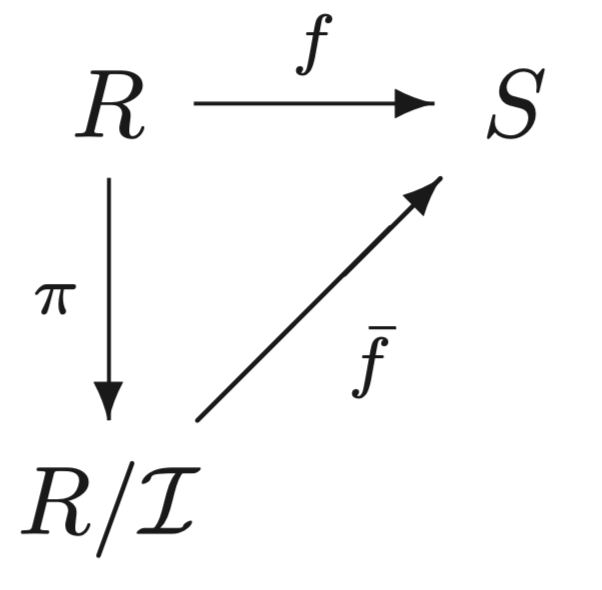
\includegraphics[width=0.2\textwidth]{Figs/3.png}
\end{figure}
We would like to find a ring homomorphism $\bar{f}: R / \mathcal{I} \rightarrow S$ that makes the diagram \tb{commute}, namely
\begin{align*}
f(a)=\bar{f}(\pi(a))
\end{align*}
for all $a \in R$.
\begin{thmx}\bfs{Factor Theorem for Rings}
Any ring homomorphism $f$ whose kernel $K$ contains $\mathcal{I}$ can be factored through $R / \mathcal{I}$. In other words, there is a \tb{unique ring homomorphism} $\bar{f}: R / \mathcal{I} \rightarrow S$ such that $\bar{f} \circ \pi=f$. Furthermore
\begin{enumerate}
    \item $\bar{f}$ is an \tb{epimorphism} if and only if $f$ is.
    \item $\bar{f}$ is a \tb{monomorphism} if and only if $K=\mathcal{I}$.
    \item $\bar{f}$ is an \tb{isomorphism} if and only if $f$ is an epimorphism and $K=\mathcal{I}$.
\end{enumerate}
\end{thmx}
\begin{proof}
Since we have already done the proof for groups in \cref{thm:aondca} with many details, here we will just mention a few important points in the proof.
Let $a+\mathcal{I} \in R / \mathcal{I}$ such that $\pi(a)=a+\mathcal{I}$ for $a \in R$. We define
\begin{align*}
\bar{f}(a+\mathcal{I})=f(a)
\end{align*}
This is the most natural way to do it, however, we need to make sure that this is indeed \tb{well-defined}, in the sense that it should not depend on the choice of the representative taken in the coset. Let us thus take another representative, say $b \in a+\mathcal{I}$. Since $a$ and $b$ are in the same coset, they satisfy $a-b \in \mathcal{I} \subset K$, where $K=\operatorname{Ker}(f)$ by assumption. Since $a-b \in K$, we have $f(a-b)=0$ and thus $f(a)=f(b)$.

Now that $\bar{f}$ is well defined, it is an easy computation to check that $\bar{f}$ inherits the property of ring homomorphism from $f$.
The rest of the proof works exactly the same as for groups as in \cref{thm:aondca}.
\end{proof}




\subsection{Integral Domain, Entire, (skew) Field: Properties of Elements of Rings}\label{sec:Entire}

\begin{defa}\bfs{invertible; unit}
  Let $R$ be a ring. An element $a \in R$ is said to be \tb{invertible}, or a \tb{unit}, if it has a \tb{multiplicative inverse}, i.e. $\exists a^{\prime} \in R$ such that $a^{\prime} a=a a^{\prime}=1$. \begin{enumerate}
      \item We know that such an inverse is unique if it exists, hence we shall write it as $a^{-1}$. 
      \item \tb{Note that when $1 \neq 0$, $0$ is never invertible. Again, when $1 \neq 0$ (i.e. ring is non-trivial), if $x$ is invertible then $x\ne 0$} (See \cref{thm:incnzcd}, \cref{thm:dsoanfda}).
      \item We denote the set of units in $R$ by $R^{*}$.
  \end{enumerate}
\end{defa} 
\begin{rema}\bfs{clarify}
\begin{enumerate}
\item From group definition we need then to the left and right additive inverse to be the same. However, in \tb{any} ring $R$, if $a$ has \tb{both} a left and a right inverse, then \tb{the left and right inverses are the same and the element is a unit.}

If $ca=ab=1$, we have
\begin{align*}
b=1 \cdot b=(c a) b=c(a b)=c \cdot 1=c
\end{align*}
Since $b=c$, then $c a=b a=a b=1$, so $b=c=a^{-1}$, as desired.
    \item However, \tb{a ring element with a left inverse may have but no right inverse}. Example: Take the ring of linear operators on the space of polynomials. Then consider (formal) integration and differentiation. Integration is injective but not surjective. Differentiation is surjective but not injective. See also the proof of \cref{lem:oqneqdd}.
\end{enumerate}
\end{rema}
\begin{lema}\label{lem:omdnqnbee}
For any ring $R,\left(R^{*}, \times\right)$ is a group.
\end{lema}

\begin{defa}\bfs{{division ring}; skew field; field}
  A \tb{non-trivial} ring $R$ in which every non-zero element is invertible $($ i.e $R \backslash\{0\}=$ $R^{*}$ ) is called a \tb{division ring} (or \tb{skew field}). If $R$ is a \tb{commutative} division ring then $R$ is called a \tb{field}.
\end{defa} 
\begin{exma}
  $\GL_{n}(\mathbb{R})$ is \tb{skew field} but not commutative.
\end{exma}
\begin{rema}$\quad$

\begin{enumerate}
    \item $(\mathbb{Q},+, \times)$ is the canonical example of a field. Other natural examples include $(\mathbb{R},+, \times),(\mathbb{C},+, \times)$ and $(\mathbb{Z} / p \mathbb{Z},+, \times)$, where $p$ is a prime number. 
    \item All of linear algebra (except the issue of eigenvalues existing) can be set up over an arbitrary field. All proofs are exactly the same, we never used anything else about $\mathbb{R}$ or $\mathbb{C} .$
\end{enumerate}
\end{rema}

\begin{exma}
  
  The collection of linear maps from $\mathbb{R}^{n}$ to $\mathbb{R}^{n}$ is the set $\mathbb{M}_{n \times n}\left(\mathbb{R}^{n}\right)$ is a ring but not a skew field (division ring).
\end{exma}


\begin{defa}\bfs{zero-divisor}
  Let $R$ be a \tb{non-trivial} ring. Given $a \in R \backslash\{0\}$, if there exists $b \in R \backslash\{0\}$ such that $a b=0$ or $b a=0$, then $a$ is said to be a \tb{zero-divisor}. Note that \tb{0 is not a zero-divisor.}
\end{defa}


\begin{exma}
  In an arbitrary ring it is possible that two non-zero elements can multiply to give zero. For example, in $\mathbb{M}_{2 \times 2}(R)$, the non-zero matrices
\begin{align*}
A=\left(\begin{array}{ll}
0 & 1 \\
0 & 0
\end{array}\right) \text { and } B=\left(\begin{array}{ll}
0 & 2 \\
0 & 0
\end{array}\right)
\end{align*}
multiply to give the zero matrix.
\end{exma}
  \begin{defa}\bfs{entire (domain); integral domain}
   A \tb{non-trivial} ring $R$ with \tb{no zero divisors} is said to be \tb{entire} or \tb{domain}; a \tb{commutative} domain is called an \tb{integral domain}. More concretely: 
   
   \centerline{$R$ is \tb{domain} if and only if $1 \neq 0$ and $\forall x, y \in R, x y=0 \Rightarrow x=0$ or $y=0$.}
\end{defa}
\begin{exma}
$(\mathbb{Z},+, \times),(\mathbb{Q},+, \times)$ are integral domains. $(\mathbb{Z} / m,+, \times)$ is an integral domain $\Longleftrightarrow m$ prime. The above example shows that $\mathbb{M}_{2}(\mathbb{R})$ is not integral domain.
\end{exma}

\begin{thma}
 A ring $R$ is domain $\Longleftrightarrow$ its set of non-zero elements forms a monoid under multiplication. In other words,  $R$ is domain $\Longleftrightarrow R \backslash\{0\}$ is \tb{closed under multiplication}, i.e., a monoid.
\end{thma}
\begin{proof}
In any ring $R$ observe that if $x, y \in R$ are two non-zero divisors then by definition $x y \in R$ must be a non-zero divisor. Hence, If $R$ is non-trivial the non-zero divisors of $R$ are a monoid under multiplication. If $R$ is entire the set of non-zero divisors is precisely $R \backslash\{0\}$, which implies it is a monoid under multiplication.

Conversly if $R \backslash\{0\}$ is a monoid then firstly it is non-empty so $R$ is non-tivial. But if $x, y \in R \backslash\{0\}$ then $x y \in R \backslash\{0\}$. Hence $R$ is entire by definition.
\end{proof}


\begin{cora}\label{cora:field_id}
Any \tb{field} $F$ is an \tb{integral domain}.
\end{cora}
\begin{proof}
If $x, y \in F, x \neq 0 \neq y$ then $\exists x^{-1}, y^{-1} \in F$ such that $x x^{-1}=x^{-1} x=1=y y^{-1}=y^{-1} y$,
therefore \tb{$x y$ is invertible so is non-zero.} Hence, non-zero elements are closed under multiplication, so $F$ is entire. $F$ is a field so $F$ is commutative, so it is an integral domain.
\end{proof}
\begin{cora}
Any \tb{skew field} $F$ is an \tb{entire} ring.
\end{cora}
\begin{rema}\label{rema:can_law}
Note \emph{entire} and \emph{invertible} are two different properties.  In rudin it directly proves field has the entire property. The key is that roughly speaking, we have invertile $\Rightarrow$ entire.

% II x,y\ne 0 in section 2, in rudin it use field to proof. It is two difff perety ,one is entire , one is skew field.
% entire vs invertibla.
% inverse of Corollary. finite  
% \end{rema}
\end{rema}
\begin{cora}{\bfs{Cancel Law of Ring}}\label{cora:ringcan}
Let $R$ be a ring. If $c \in R$ is \tb{not a zero-divisor}, then for any $a, b \in R$ such that $c a=c b$ or $a c=b c$, then $a=b$.

This is because $c a-c b=c(a-b)$ and $a c-b c=(a-b) c$. In particular, \tb{if $R$ is entire, then we can "cancel" any non-zero element.} It is important to note that we cannot do this in an arbitrary ring.
\end{cora}
\begin{rema}
See also \cref{rem:dinfdaf} for comparison of cancel law for ring and cancel law for group.
\end{rema}

We next have the other direction of \cref{cora:field_id}:
\begin{thma}
Every \tb{finite integral domain} $R$ is a \tb{field}.
\end{thma} 
\begin{proof}
We need to show that $R^{*}=R \backslash\{0\}$. Let $a \in R \backslash\{0\}$. Define the following map of sets:
\begin{align*}
\begin{aligned}
\psi: R \backslash\{0\} & \rightarrow R \backslash\{0\} \\
r & \mapsto r a .
\end{aligned}
\end{align*}
$\psi$ is well define because $R$ is an integral domain. By the cancellation law for integral domains, we know that given $r_{1}, r_{2} \in R, r_{1} a=r_{2} a \Rightarrow r_{1}=r_{2} \Rightarrow \psi$ injective. Since $R \backslash\{0\}$ is finite, $\psi$ is surjective $\Rightarrow \exists b \in R \backslash\{0\}$ such that $b a=a b=1$. Hence $a$ has a multiplicative inverse. Therefore, $R^{*}=R \backslash\{0\}$.
\end{proof}
\begin{cora}\bfs{Wedderburn's Little Theorem}\label{cor:ndnad}We have
\begin{enumerate}
\item Every \tb{finite domain} $R$ is a \tb{skew field}. 
    \item More generally, \tb{Wedderburn's little theorem} states that every finite domain is a field. In other words, for \tb{finite} rings, \tb{there is no distinction between domains, division rings and fields.}
\end{enumerate}
\end{cora}



We next show several applications using Cancellation Law of Ring \cref{cora:ringcan}
\begin{lema}
If matrix $AB=1$, then $BA=1$
\end{lema}
\begin{proof}
Since $A B=I$ then $B=B(A B)=(B A) B$. Note from $A B=I$ that $1=\operatorname{det}(A B)=\operatorname{det}(A) \operatorname{det}(B)$ so $\operatorname{det}(B) \neq 0$.
So by $(B A) B=B$ we have:
$(B A-I) B=0$. Since $\operatorname{det}(B) \neq 0\Leftrightarrow B$ is invertible (i.e. $Bx=0\Leftrightarrow x=0$) $\Leftrightarrow B$ is not a 0 divisor. So $B A=I$.
\end{proof}
\subsection{Polynomial Rings}
\subsubsection{One Variable Polynomial Ring}
We consider \tb{ring $R$.}
\begin{defa}\bfs{polynomial ring}
 The polynomial ring in $X$ with \tb{cofficients in a ring $R$} consists of formal expressions of the form:
\begin{align*}
g(X)=b_{0}+b_{1} X+b_{2} X^{2}+\cdots+b_{m} X^{m}, b_{i} \in R, m \in \mathbb{N}
\end{align*}
If $f(X)=a_{0}+a_{1} X+\cdots+a_{n} X^{n}$ is another polynomial then we define that 
$$f(X)=g(X) \Longleftrightarrow a_{i}=b_{i}, \forall i$$ 
Note that we set $a_{i}=0$ if $i>n$ and $b_{j}=0$ if $j>m$. 
We refer to $X$ as the \tb{indeterminant}.

\tb{Addition $+$ and multiplication $\times$} are defined by the rules
\begin{enumerate}
    \item $f(X)+g(X)=\left(a_{0}+b_{0}\right)+\left(a_{1}+b_{1}\right) X+\cdots+\left(a_{n}+b_{n}\right) X^{n}($ if $m \leq n)$
    \item $f(X) \times g(X)=\left(a_{0} b_{0}\right)+\left(a_{0} b_{1}+a_{1} b_{0}\right) X+\left(a_{0} b_{2}+a_{1} b_{1}+a_{2} b_{0}\right) X^{2}+\cdots+a_{n} b_{m} X^{n+m}$
\end{enumerate}
We will denote this ring by $R[X]$. 
\end{defa}
\begin{rema}\bfs{explanation}
\begin{enumerate}
    \item In general $f\times g \ne g\times f$
    \item Note that here we may view a polynomial as \tb{a sequence with only finite manly nonzero elements}. 
\end{enumerate}
\end{rema}
\begin{lema}
Check the above $R[X]$, the set of polynomials in $X$ with coefficients in $R$, has  the ring structure with
\begin{enumerate}
    \item $0$ and $1$ in $R$ are the zero and one in $R[X]$, i.e. $m=0$
    \item If further $R$ commutative $\Rightarrow R[X]$ commutative ring.
\end{enumerate}
\end{lema}
\begin{proof}
The Abelian group properties of $R[X]$ follows easily from the Abelian group properties of $R$ and the coefficients from all from $R$. We next prove the the associated property in the monoid of the multiplication: $(f\times g)\times h = f\times (g\times h)$, where $f=\sum a_iX^i$, $g=\sum b_iX^i$ and $h=\sum c_iX^i$.
\begin{align*}
  (f\times g)\times h  &= (\sum_k\sum_{i+j=k}a_ib_jX^k)(\sum c_lX^l)\\ 
  &= \sum_w\sum_{i+j+l=w}a_ib_jc_lX^w
\end{align*}
We also get $$f\times (g\times h)= \sum_w\sum_{i+j+l=w}a_ib_jc_lX^w.$$ Compare the $w$-th item, we get they are same.
Finally the distributive law $(f+ g)\times h= f\times h + g\times h$ is also obvious. Commutative case is easy.
\end{proof}


$\bullet$ There is a natural embedding:
\begin{align*}
\begin{aligned}
\phi: R & \longrightarrow R[X] \\
a & \longrightarrow a\left(\text { polynomial with } m=0 \text { and } a=a_{0}\right)
\end{aligned}
\end{align*}

$\bullet$ Given $f(X) \in R[X]$ we can construct a map (of sets):
\begin{align*}
\begin{aligned}
\varphi_{f}: R & \longrightarrow R \\
a & \mapsto f(a),
\end{aligned}
\end{align*}
where $f(a) \in R$ is the element of $R$ given be replacing $X$ by $a$. 

% \begin{rema}
% If $R$ is a subring of $S$, given a subset $M=\{m_i\}\subseteq S\backslash R$, we can define a new ring using the map
% \begin{align*}
% \begin{aligned}
% \varphi_{f}: M & \longrightarrow S \\
% a & \mapsto f(a),
% \end{aligned}
% \end{align*}
% But note, here we have $f\times g =$
% \end{rema}

\begin{defa}\bfs{root (zero)}
 Let $R$ be a ring and $f \in R[X]$ be a {non-zero polynomial}. We say that $a \in R$ is a \tb{root}, or \tb{zero}, of $f$ if $f(a)=0$.
\end{defa}
\begin{defa}\bfs{degree, monic, constant}
 Let $R$ be a ring and $f \in R[X]$ be a non-zero polynomial. Hence we may write $f=c_{n} X^{n}+c_{n-1} X^{n-1}+\cdots+c_{0}, c_{i} \in R, c_{n} \neq 0$.\begin{enumerate}
     \item We call $n$ the \tb{degree} of $f$ and write $\deg(f)=n$.
     \item  If in addition $c_{n}=1$, we say that $f$ is \tb{monic}. 
     \item Elements of degree $0$ are called \tb{constant polynomials}.
 \end{enumerate} 
\end{defa}
\begin{thma}\label{thm:enafdz}
 If $R$ is \tb{entire} then $R[X]$ satisfies:
 \begin{enumerate}
     \item $\forall f, g \in R[X] \backslash\{0\}, \deg(f+g) \leq \max \{\deg(f), \deg(g)\}$
     \item $\forall f, g \in R[X] \backslash\{0\} \Rightarrow f g \neq 0$ and $\deg(f g)=\deg(f)+\deg(g)$.
 \end{enumerate}
\end{thma}
\begin{proof}
By the definition of degree, 1). is clear. For 2):
Let $\deg(f)=n, \deg(g)=m$. Then suppose $a_{n}, b_{m}$ the leading coefficients of $f$ and $\mathrm{g}$ respectively. Hence $f g$ has maximal power of $X$ given by $a_{n} b_{m} X^{n+m}$. As $R$ is entire, $a_{n} b_{m} \neq 0 \Rightarrow$ ``$ \deg(f g)=n+m=\deg(f)+\deg(g)$, and $f g \neq 0$.''
\end{proof}
\begin{cora}\label{cor:indgad}We have that
\begin{enumerate}
    \item \tb{$R$ entire $\Rightarrow R[X]$ entire. }
    \item \tb{$R$ an integral domain $\Rightarrow R[X]$ an integral domain.}
\end{enumerate}
\end{cora}
\begin{proof}
From the last sentence of the above proof.
\end{proof}

\begin{thmx}\label{thm:adiqbnee}
Let $A$ and $B$ be rings and let $\sigma: A \rightarrow B$ be a \tb{ring homomorphism} with kernel $K$. Define (with the abuse of notation, better to use for example $\bar{\sigma}$) $\sigma: A[x] \rightarrow B[x]$ by
\begin{align*}
\sigma\left(a_{0}+a_{1} x+\cdots a_{n} x^{n}\right)=\sigma\left(a_{0}\right)+\sigma\left(a_{1}\right) x+\cdots+\sigma\left(a_{n}\right) x^{n}
\end{align*}
We have $\sigma$ is a \tb{ring homomorphism} from $A[x]$ to $B[x]$.
\end{thmx}


\begin{proof}
Easy, just check the properties of ring homomorphism \cref{def:donacca} are satisfied, all from the ring homomorphism of $h$.
\end{proof}
\begin{corx}\label{cor:odnarea}
   For $\alpha \in A$, and $f\in A[X]$ we have 
   \begin{align*} \sigma(f(\alpha)) &=\sigma\left(c_{n} \alpha^{n}+c_{n-1} \alpha^{n-1}+\cdots+c_{1} \alpha+c_{0}\right) \\ &=\sigma\left(c_{n}\right) \sigma(\alpha)^{n}+\sigma\left(c_{n-1}\right) \sigma(\alpha)^{n-1}+\cdots+\sigma\left(c_{1}\right) \sigma(\alpha)+\sigma\left(c_{0}\right) \\ &=(\sigma f)(\sigma(\alpha)) . \end{align*}
  So if $f(\alpha)=0$ then $(\sigma f)(\sigma(\alpha))=\sigma(f(\alpha))=\sigma(0)=0$, so $\sigma$ sends any \tb{root} $\alpha$ of $f(X)$ in $A$ to a \tb{root} $\sigma(\alpha)$ of $(\sigma f)(X)$ in $B$.
\end{corx}

\subsubsection{Multi Variable Polynomial Ring: }
\begin{defa}\bfs{multi-variable polynomial ring}
 Since $R[X]$ is still a ring. Inductively, we can define
\begin{align*}
R\left[X_{1}, \cdots, X_{n}\right]=R\left[X_{1}, \cdots, X_{n-1}\right]\left[X_{n}\right].
\end{align*}
Note $f \in R\left[X_{1}, \cdots, X_{n}\right]$ has a unique expression of the form
\begin{align*}
f=\sum a_{i_{1} \cdots i_{n}} X^{i_{1}} \cdots X_{n}^{i_{n}}\left(a_{i_{1} \cdots i_{n}} \in R\right)
\end{align*}
where the sum is finite.
\end{defa}
\begin{defa}\bfs{monomials}
 Expressions of the form $m_{(i)}=X_{1}^{i_{1}} \cdots X_{n}^{i_{n}}$ are called \tb{monomials}.
\end{defa}
\begin{cora}\label{cor:ncnkd}Analogous to \cref{cor:indgad}, We have that
\begin{enumerate}
    \item \tb{$R$ entire $\Rightarrow R[X_1,X_2,\cdots,X_n]$ entire. }
    \item \tb{$R$ an integral domain $\Rightarrow R[X_1,X_2,\cdots,X_n]$ an integral domain.}
\end{enumerate}
\end{cora}
\subsection{Field of Fractions}
In this section, we \tb{construct a field from any integral domain} and contains the integral domain as a subset (i.e. embedding the integral domain to a field), analogous to the \tb{construct of $\bbQ$ from $\bbZ$}:

\subsubsection{Recall the $\bbQ$}
\begin{enumerate}
    \item Elements in $\bbQ$ often are in the form of $\frac{a}{b}$ with $a, b \in \mathbb{Z}, b \neq 0$. This is not unique. $\frac{a}{b}=\frac{c}{d} \Longleftrightarrow a d-b c=0$.
    \item In $\bbQ$, we define $+$ and $\times$ by the following rules:
    \begin{enumerate}
        \item $\frac{a}{b}+\frac{c}{d}=\frac{a d+c b}{b d}$
        \item $\frac{a}{b} \times \frac{c}{d}=\frac{a c}{b d}$
    \end{enumerate}
\item We should therefore think of elements of $\mathbb{Q}$ as pairs of integers $(a, b)$ such that $b \neq 0$, \tb{up to an equivalence relation:}
\begin{align*}
(a, b) \sim(c, d) \Longleftrightarrow a d-c b=0
\end{align*}
Hence, $\mathbb{Q}$ can be thought of as $(\mathbb{Z} \times \mathbb{Z} \backslash\{0\} / \sim)$. 
\item The well-definedness of $+$ and $\times$ is not obvious and needs checking, i.e. choosing different elements of the same equivalence class should give the same results.
\end{enumerate}

\subsubsection{Generalise the Construction on Integral Domain}
\begin{defa}\bfs{Elements in the Field}
 Let $R$ be an \tb{integral domain}. We define the \tb{equivalence relation} (See \cref{lem:odmnnbzfr}) on $R \times R \backslash\{0\}$ by:
\begin{align*}
(a, b) \sim(c, d) \Longleftrightarrow a d-b c=0
\end{align*}
Let us denote the equivalence classes by $(R \times(R \backslash\{0\})) / \sim$.  For $(a, b) \in R \times(R \backslash\{0\})$ we often denote the equivalence class containing $(a, b)$ by $\frac{a}{b}$.
\end{defa}
\begin{lema}\label{lem:odmnnbzfr}$\sim$ is indeed an equivalence relation.
\end{lema} 
\begin{rema}
Note, properties (e.g.commutative, cancel law) of integral domain are quite crucial for the equivalence.
\end{rema}
\begin{proof}
\begin{enumerate}
    \item $(a, b) \sim(a, b)$ as $a b-a b=0$ since $R$ is commutative.
    \item  $(a, b) \sim(c, d) \Rightarrow a d-b c=0 \Rightarrow  cb-da=0 \Rightarrow(c, d) \sim(a, b)$ since $R$ is commutative.
    \item Let $(a, b) \sim(c, d)$ and $(c, d) \sim(e, f)$. Then $a d-b c=0, c f-d e=0$. Consider
\begin{align*}
\begin{aligned}
(a f-b e) d &=a d f-b e d \\
&=f(a d-b c)+b(c f-d e) \\
&=f 0+b 0=0
\end{aligned}
\end{align*}
$d \neq 0 \Rightarrow a f-b e=0 \Rightarrow(a, b) \sim(e, f)$
\end{enumerate}
\end{proof}


\begin{defa}\bfs{$+$ and $\times$ in the Field}
Let us define multiplication and addition on $R \times R \backslash\{0\} / \sim$ by 
\begin{align*}
\frac{a}{b}+\frac{c}{d}=\frac{a d+b c}{b d} \quad \frac{a}{b} \times \frac{c}{d}=\frac{a c}{b d}
\end{align*}
\end{defa}
\begin{lema}
 $+$ and $\times$ are well-defined on $(R \times(R \backslash\{0\})) / \sim$.
\end{lema}
\begin{proof}
The first thing to note is that if $b, d \in R \backslash\{0\} \Rightarrow b d \in R \backslash\{0\}$ as $R$ is an integral domain. We just need to check that choosing different representatives gives the same answer.
\end{proof}
\begin{cora}\bfs{0 and 1 in the Field}We have
\begin{enumerate}
    \item The zero in $(R \times(R \backslash\{0\})) / \sim$ is given by the equivalence class containing $(0,1)$.
    \item The one in $R \times(R \backslash\{0\}) / \sim$ is given by the equivalence class containing $(1,1)$.
\end{enumerate}
\end{cora}
\begin{proof}
For all $(a, b) \in(R \times(R \backslash\{0\}))$,
\begin{align*}
\frac{a}{b}+\frac{0}{1}=\frac{a \times 1+b \times 0}{b \times 1}=\frac{a}{b} .
\end{align*}
\begin{align*}
\frac{a}{b} \times \frac{1}{1}=\frac{a 1}{b 1}=\frac{a}{b}
\end{align*}
Both operations are clearly commutative because $R$ is commutative. Hence we are done.
\end{proof}
\begin{thma}
 $(R \times(R \backslash\{0\})) / \sim$ is a field.
\end{thma}
\begin{rema}\label{rem:zncnffe}
It is a straight forward exercise to check that under these operations $(R \times(R \backslash\{0\})) / \sim$ is a commutative ring. Also observe that 
\begin{enumerate}
    \item $(a, b) \in(R \times(R \backslash\{0\}))$ is in the \tb{zero class} if and only if $a=0$.
    \item Similarly $(a, b)$ give the \tb{one class} if and only in $a=b$. 
\end{enumerate} 
This is good. It's the same as in $\mathbb{Q}$, so we've done something right.
\end{rema}
\begin{proof}
We just need to check non-zero elements have multiplicative inverses. Let $\frac{a}{b} \in(R \times$ $(R \backslash\{0\})) / \sim$ be non-zero. By \cref{rem:zncnffe} this implies that $a \neq 0$. Hence $\frac{b}{a} \in(R \times(R \backslash\{0\})) / \sim$. But
\begin{align*}
\frac{a}{b} \times \frac{b}{a}=\frac{a b}{a b}=\frac{1}{1} .
\end{align*}
Hence we are done. 
\end{proof}
\begin{defa}\bfs{Field of Fraction}From now on we denote the constructed field as:
\begin{enumerate}
    \item Let $R$ be an integral domain. The \tb{field of fractions} of $R$ is the field 
    $$\Frac(R)\coloneqq(R \times(R \backslash\{0\})) / \sim.$$
    \item Given an integral domain $R$ and indeterminants $\left\{X_{1}, \cdots, X_{n}\right\}$, we know from \cref{cor:ncnkd} that $R\left[X_{1}, \cdots, X_{n}\right]$ is an integral domain. We define
\begin{align*}
R\left(X_{1}, \cdots, X_{n}\right):=\operatorname{Frac}\left(R\left[X_{1}, \cdots, X_{n}\right]\right)
\end{align*}
\end{enumerate}
\end{defa}
\begin{exma}
The canonical example is $\operatorname{Frac}(\mathbb{Z})=\mathbb{Q}$.
\end{exma}


\begin{thma}
The map
\begin{align}
\begin{aligned}
\phi: R & \rightarrow \operatorname{Frac}(R) \\\label{eq:pmdmfd}
a & \mapsto \frac{a}{1}
\end{aligned}
\end{align}
is an embedding.
\end{thma}
\begin{proof}
 We need to check that $\phi$ is a homomorphism first.
 \begin{enumerate}
     \item Given $a, b \in R, \phi(a+b)=\frac{a+b}{1}=\frac{a}{1}+\frac{b}{1}=\phi(a)+\phi(b)$.
     \item Given $a, b \in R, \phi(a b)=\frac{a b}{1}=\frac{a}{1} \times \frac{b}{1}=\phi(a) \phi(b)$.
     \item  $\phi(1)=\frac{1}{1}$
 \end{enumerate}
To check it is injective we just need to show that the kernel (as a homomorphism of Abelain groups) is trivial.
$\phi(a)=\frac{a}{1}=\frac{0}{1} \Longleftrightarrow a=0$. Thus the kernel is trivial and so $\phi$ is injective.
\end{proof}
\begin{cora}
Every integral domain may be embedded in a field.
\end{cora} 
\begin{cora}
Let $R$ be a field. The natural embedding \cref{eq:pmdmfd} $R \rightarrow \Frac(R)$ is an \tb{isomorphism}.
\end{cora}
\begin{proof}
 We must show $\phi$ is \tb{surjective}. Let $\phi$ denote the natural embedding $R \rightarrow \Frac(R)$. Let $\frac{a}{b} \in \operatorname{Frac}(R)$. $R$ is a field so there exist $b^{-1}$, a multiplicative inverse to $b$. But $\frac{a}{b}=$ $\frac{a b^{-1}}{1}=\phi\left(a b^{-1}\right)$. Hence $\phi$ is surjective. Therefore $\phi$ is an isomorphism.
\end{proof}

\subsection{Characteristic: Additive Order of Elements}
Let $R$ be \tb{entire} (non-trivial with no zero-divisors). 

% Recall that $(R,+)$ is an abelian group, hence given $a \in R$ we may talk about its additive order. 
\begin{thma}\label{thm:daiocd}
 In an entire ring $R$, the additive order of every non-zero element is the \tb{same}. In addition, if this order is \tb{finite} then it is \tb{prime}.
\end{thma}
\begin{proof}
 Let $a \in R \backslash\{0\}$ be of finite (additive) order $k>1$, i.e. $k$ is minimal such that $k a=$ 0 . This implies $\left(k \times 1_{R}\right) a=0 \Rightarrow k \times 1_{R}=0$ as $R$ is entire and contains no zero-divisors. Therefore if we choose $b \in R \backslash\{0\}$ then $k b=\left(k \times 1_{R}\right) b=0 \times b=0 \Rightarrow$ every element has order dividing $k$. Choosing $a$ with minimal order $k>1$ ensures that every nonzero element must have order $k$. If no element has finite order, all elements must have infinite order.
Now assume that $1_{R} \in R$ has finite order $k>1$ and that we have factored $k=r s$ in $\mathbb{N}$. Then $k 1_{R}=(r s) 1_{R}=\left(r 1_{R}\right)\left(s 1_{R}\right)=0$ (See \cref{lem:odnndsaff}). Since $R$ entire, either $r 1_{R}=0$ or $s 1_{R}=0$. However, since $k$ is the minimal order of $1_{R}, r=k$ or $s=k$. Therefore, $k$ must be prime.
\end{proof}


\begin{defa}\bfs{Characteristic}
Suppose $R$ an \tb{entire} ring.
\begin{enumerate}
    \item $R$ has \tb{characteristic zero} if all of its non-zero elements have \tb{infinite} additive order, denoted $\charac(R)=0$.
    \item If all non-zero elements of $R$ are of additive order $p \in \mathbb{N}$, then $R$ is \tb{characteristic $p$}, or  $\charac(R)=p$. In this case, $R$ is \tb{finite} characteristic.
\end{enumerate} 
\end{defa}

\begin{rema}\bfs{explanation}
\begin{enumerate}
    \item Recall that in \cref{rem:oindnaf} we have mentioned that:
$$\mathbb{Z} / m \mathbb{Z}\text{ is a field }\Longleftrightarrow m \text{ is a prime.}$$
\cref{thm:daiocd} can be viewed as the \tb{generalization} of \cref{rem:oindnaf} where prime is from \cref{rem:oindnaf}, and same order of all elements follows from \cref{lem:iondfdagtv}.
\item  Under finite assumption, in general we have field $\Leftrightarrow$ entire (See \cref{cor:ndnad}), we therefore have that: 

\centerline{\tb{The element in any finite field or entire must have prime order.}}

\item Note this \tb{does not} means any finite field have prime order. Instead, we have $p^n$ as shown in \cref{thm:Lnbd}.
\end{enumerate}
\end{rema}
\begin{thma}\label{thm:Lnbd}
Let $F$ be a finite field. The order of $F$ is always of order $p^{n}$ where $p$ is prime.
\end{thma}
\begin{proof} Directly follows from \cref{lem:djfdacf}. Here we give a detailed proof again, but the proof idea is the same:

 Let $p$ be the characteristic of a finite field $F$. Then since 1 has order $p$ in $(F,+)$, we know that $p$ divides $|F|$. Now let $q \neq p$ be any other prime dividing $|F|$. Then by \cref{thm:sylow} and \cref{lem:iondfdagtv}, there is an element $x \in F$ whose order in $(F,+)$ is $q$.
 
Then $q  x=0$. But we also have $p  x=0$. Now since $p$ and $q$ are relatively prime, we can find integers $a$ and $b$ such that $a p+b q=1$.

Thus $(a p+b q)  x=x$. But $(a p+b q)  x=a (p  x)+b (q  x)=0$, giving $x=0$, which is not possible since $x$ has order at least 2 in $(F,+)$.
So there is no prime other than $p$ which divides $|F|$.
\end{proof}



\begin{exma}
When studying abstract fields, the characteristic is very important.
Eg. $\mathbb{Q}, \mathbb{R}, \mathbb{C}$ are all fields (hence entire) of characteristic zero.
\end{exma} 
\begin{defa}\bfs{$\mathbb{F}_{p}$}
If $p$ is a prime number $\mathbb{Z} / p \mathbb{Z}$ is a field of characteristic $p$. We denote this later field by $\mathbb{F}_{p}$.
\end{defa}
\begin{thma}
There is an embedding of $\mathbb{Q}$ in any field $F$ of characteristic $0 .$
\end{thma}
\begin{proof}
 Let $1_{F}$ denote the multiplicative identity in $F$. Let $0_{F}$ denote the additive identity in $F$. We must find a suitable embedding of $\mathbb{Q}$ in $F$. 
 
\tb{Step 1:} Because $\operatorname{char}(F)=0$, the natural map homomorphism:
\begin{align*}
\begin{gathered}
\phi: \mathbb{Z} \rightarrow F \\
n \mapsto n 1_{F}
\end{gathered}
\end{align*}
is \tb{injective}. We claim that it is a homomorphism (of rings). Let $a, b \in \mathbb{Z}$, then $\phi(a b)=$ $a b 1_{F}=a b 1_{F} 1_{F}=a 1_{F} b 1_{F}=\phi(a) \phi(b) ; \phi(a+b)=(a+b) 1_{F}=a 1_{F}+b 1_{F}=\phi(a)+\phi(b)$. $\phi(1)=1_{F}$. Thus $\phi$ is an \tb{injective homomorphism.}

\tb{Step 2:} Now we will extend this notion to $\mathbb{Q}$. 

We define the following map:
\begin{align*}
\begin{gathered}
\psi: \mathbb{Q} \rightarrow F \\
\frac{n}{m} \mapsto \phi(n) \phi(m)^{-1}
\end{gathered}
\end{align*}
We must check that $\psi$ is well defined and is an embedding.
For $a, b, n, m \in \mathbb{Z}, \frac{n}{m}=\frac{a}{b} \Rightarrow n b-a m=0$. Therefore
\begin{align*}
\begin{aligned}
\phi(n b-a m)=\phi(0)=0_{F}=\phi(n b)-\phi(a m) & \Rightarrow \phi(n b)=\phi(a m) \\
& \Rightarrow \phi(n) \phi(b)=\phi(a)\psi(m) \\
& \Rightarrow \phi(n) \phi(m)^{-1}=\phi(a) \phi(b)^{-1} \\
& \Rightarrow \psi\left(\frac{n}{m}\right)=\psi\left(\frac{a}{b}\right)
\end{aligned}
\end{align*}
This shows that $\psi$ is well defined.
Next: $\psi$ is a homomorphism.
\begin{align*}
\begin{aligned}
\psi\left(\frac{a}{b}+\frac{n}{m}\right) &=\psi\left(\frac{a m+b n}{b m}\right) \\
&=(\phi(a) \phi(m)+\phi(b) \phi(n)) \phi(b m)^{-1} \\
&=\phi(a) \phi(b)^{-1}+\phi(n) \phi(m)^{-1} \\
&=\psi\left(\frac{a}{b}\right)+\psi\left(\frac{n}{m}\right)
\end{aligned}
\end{align*}
\begin{align*}
\begin{aligned}
\psi\left(\frac{a}{b} \frac{n}{m}\right) &=\psi\left(\frac{a n}{b m}\right) \\
&=\phi(a n) \phi(b m)^{-1} \\
&=\phi(a) \phi(n) \phi(b)^{-1} \phi(m)^{-1} \\
&=\phi(a) \phi(b)^{-1} \phi(n) \phi(m)^{-1} \\
&=\psi\left(\frac{a}{b}\right) \psi\left(\frac{n}{m}\right)
\end{aligned}
\end{align*}
By definition $\psi\left(\frac{1}{1}\right)=1_{F}$. Thus we have a \tb{homomorphism}. We claim that it is \tb{injective}. We must show that the kernel (as a homomorphism of Abelian groups) is trivial. Let $\frac{n}{m} \in \mathbb{Q}$ such that $\psi\left(\frac{n}{m}\right)=0$. Then $\phi(n) \phi(m)^{-1}=0 \Rightarrow \phi(n)=0 \Rightarrow n=0$ as $\phi$ was already shown to be injective. Therefore the kernel is trivial, so $\psi$ is an embedding.
\end{proof}


\begin{thma}
There is an embedding of $\mathbb{F}_{p}$ in any field $F$ of characteristic $p$, where $p$ is prime. 
\end{thma} 
\begin{proof}
 Note that $\left\{0_{F}, 1_{F}, \cdots,(p-1) 1_{F}\right\} \subseteq F$ is closed under $+$ and $\times$, hence forms a subring. Clearly $\mathbb{F}_{p}$ is isomorphic to this subring under the embedding
\begin{align*}
\begin{aligned}
\psi: \mathbb{F}_{p} & \longrightarrow F \\
{[\mathrm{a}] } & \longrightarrow a 1_{F}
\end{aligned}
\end{align*}
\end{proof}

\subsection{Ring Extensions}
Let $R$ be a subring of \tb{commutative ring} $S$. 
\begin{defa}\bfs{Ring Extension}\label{def:qondadfd}
The \tb{ring extension} of $R$ by $\left\{\alpha_{1}, \cdots, \alpha_{n}\right\} \subset S$ is the subring
\begin{align*}
R\left[\alpha_{1}, \cdots, \alpha_{n}\right]=\left\{f\left(\alpha_{1}, \cdots, \alpha_{n}\right) \mid f \in R\left[X_{1}, \cdots, X_{n}\right]\right\}
\end{align*}
\end{defa}
\begin{lema}
 $R\left[\alpha_{1}, \cdots, \alpha_{n}\right]$ is a subring.  Further more it is the intersection of all subrings containing $R$ and the subset $\left\{\alpha_{1}, \cdots, \alpha_{n}\right\}$.
\end{lema}
\begin{rema}
So $R\left[\alpha_{1}, \cdots, \alpha_{n}\right]$ is the smallest subring containing $R$ and $\left\{\alpha_{1}, \cdots, \alpha_{n}\right\}$.
\end{rema}

\subsection{Principal, Prime and Maximal Ideals}
\begin{defa}\bfs{proper ideal}
An ideal $I \subset R$ is \tb{proper} if $I \neq R$.
\end{defa} 
\begin{lema}
 $I$ does not contain a \tb{unit} $\Longleftrightarrow$ $I \subset R$ is proper $\Longleftrightarrow$ $R / I$ is a non-trivial ring.
\end{lema}
\begin{proof}
 This is because ideal $I$ contains a \tb{unit} $\Longleftrightarrow$ $I$ contains \tb{one}.
\end{proof}
\begin{defa}\bfs{principal ideal}
Let $R$ be a \tb{commutative} ring. We say an ideal $I \subset R$ is \tb{principal} if there exist $a \in R$ such that $I=\{r a \mid r \in R\}$. In this case we write $I=(a)\coloneqq \{r a \mid r \in R\}$.
\end{defa} 
\begin{lema}
Let $R$ be a \tb{commutative} ring.  $(a)\coloneqq \{r a \mid r \in R\}$ is an ideal and it is the smallest ideal containing $a$.
\end{lema}
\begin{proof}
 From definition, it is easy to check and here \tb{commutative} is import.
\end{proof}
\begin{lema}
Let  $I = (a)$, we have 

\centerline{\tb{$I$ is proper $\Longleftrightarrow$ $a$ is not unit $\Longleftrightarrow$ $I$ does not contain unit}}
\end{lema}
\begin{proof}
Others are easy. Here we only point out if $a$ is not a unit, $1\in (a)$.
\end{proof}
\begin{defa}\bfs{prime ideal}\label{rem:dmdmfeoald}
Let $R$ be a \tb{commutative ring}. We say an ideal $I \subset R$ is \tb{prime} if it is \tb{proper}, and given $a, b \in R$ such that $a b \in I$ then either $a \in I$ or $b \in I$. In other words, the set $R\backslash I$ (not the quotient ring $R/I$) is closed under $\times$. 
\end{defa}
\begin{rema}
Later, we will see in \tb{integral domain}, 

\centerline{principle ideal $(a)$ is a \tb{prime ideal} $\Longleftrightarrow$ $a$ is a \tb{prime element}.}
\end{rema}
\begin{lema}
 Let $R$ be a \tb{commutative ring}. Let $I \subset R$ be an ideal. Then 
 
 \centerline{$I$ is \tb{prime} $\Longleftrightarrow$ $R / I$ is an \tb{integral domain}.}
\end{lema}
\begin{rema}
Analogously, if we remove the commutative condition in the definition of prime \cref{rem:dmdmfeoald}, we have under $R$ is ring,  prime $\Longleftrightarrow$ entire.
\end{rema}
\begin{proof}
$\Rightarrow$:
  $I$ is a proper ideal hence $R / I$ is non-trivial.
Observe that $R$ commutative trivially implies that $R / I$ is commutative. Let $I \subset R$ be prime and assume that $R / I$ has zero divisors. Then there exists $a, b \in R$ such that $a, b \notin I$ but $(a+I)(b+I)=0+I$. But this trivially implies that $a b \in I$. But this contradicts the fact that $I$ is prime.

$\Leftarrow$:
Assume that $R / I$ is an integral domain but $I$ is not prime. Hence we can find $a, b \in R$ such that $a b \in I$ but $a, b \notin I$. But then $(a+I)$ and $(b+I)$ are zero divisors, which is a contradiction.
\end{proof}
\begin{defa}\bfs{maximal ideal}
Let $R$ be a \tb{commutative ring}. We say that an ideal is \tb{maximal} if it is maximal among the set of proper ideals. More precisely $I \subset R$ is a \tb{maximal ideal} if given an ideal $J \subset R$ such that $I \subset J$, then either $I=J$ or $J=R$
\end{defa}
\begin{rema}
This is a partial order, so the maximal ideal may be not unique.
\end{rema}
\begin{lema}\label{lem:omdnad}
 Let $R$ be a \tb{commutative} ring. Let $I \subset R$ be an ideal. Then 
 
 \centerline{$I$ is \tb{maximal} $\Longleftrightarrow$ $R / I$ is a \tb{field}.}
\end{lema} 
\begin{proof}
$\Rightarrow$ First observe that $R$ commutative trivially implies that $R / I$ is commutative.
Assume that $I \subset R$ is maximal. Take a non-zero element of $R / I$, i.e. $a+I$ for $a \notin I$. Consider the ideal $(a) \subset R$. Consider the following new ideal:
$$
(a)+I=\{r a+b \mid r \in R, \quad b \in I\} .
$$
Note that this is certainly an ideal because it is closed under addition and scalar multiplication by all $R$. Note that by construction $I \subset(a)+I$ and $a \in(a)+I$. Hence $I$ is strictly contained in $(a)+I$. But $I$ is maximal. Hence $(a)+I=R$. Thus there exist $r \in R$ and $b \in I$ such that $r a+b=1$. Hence $(r+I)(a+I)=r a+I=1+I$. Thus $(a+I)$ has a multiplicative inverse. Hence $R / I$ is a field.

$\Leftarrow$ Assume that $R / I$ is a field. Assume that $J$ is a proper ideal of $R$ which strictly contains $I$, i.e. $I$ is not maximal. Let $a \in J$ and $a \notin I$. Thus $(a+I)$ is non-zero in $R / I$. Thus it has a multiplicative inverse. Hence there exists $b \in R$ such that $a b+I=1+I$. This implies that $a b-1 \in I$, which in turn implies that $a b-1 \in J$. But $a \in J$, hence $1 \in J$, which implies that $J=R$. This is a contradiction. Hence I is maximal.
\end{proof} 


\begin{cora}\label{cor:omadnmnee}
Let $R$ be a \tb{commutative} ring. Let $I \subset R$ be an ideal. Then 

\centerline{$I$ \tb{maximal} $\Rightarrow$ $I$ is \tb{prime}.}
\end{cora}
\begin{proof}
$I$ maximal $\Rightarrow R / I$ is a field $\Rightarrow R / I$ is an integral domain $\Rightarrow I$ prime.
\end{proof} 

\subsection{Factorisation in Integral Domains, Irreducible and Prime Elements}\label{sec:facid}

Let $R$ be a ring. In $\mathbb{Z}$, we have the "Fundamental Theorem of Arithmetic": every non-zero element of $\mathbb{Z}$ is $\pm 1$ times a unique product of prime numbers. 

If $R$ is not commutative or has zero-divisors the factorisation is not well defined or too complicated. If $c$ is a zero-divisors, $(a-b)c=0$, but we have $ac=bc$ with $a\ne b$.

$\bullet$ We assume $R$ is an \tb{integral domain}.

\subsubsection{Unique Factorization Domain, Irreducible Elements}\label{sec:infddf}
We definite the analogy concept of \tb{basic (i.e. irreducible)} divisors  in $R$ that will works similar to prime integer in $\bbZ$. Later we will define general \tb{prime element} in $R$ and show the relation between  \tb{irreducible element} and \tb{prime element}.



\begin{defa}
Let $a, b \in R$.  $a \mid b$ will mean that $\exists c \in R$ such that $b=a c$.
\end{defa}

\begin{defa}\bfs{associated}
Two non-zero elements $a, b$ in an integral domain $R$ are \tb{associated} if $a \mid b$ and $b \mid a$, i.e. $\exists c, d \in R$ such that $b=a c$ and $a=b d$.
\end{defa}
\begin{thma}\label{thm:omare}
 In $R$ an integral domain, and $a, b \in R$ be two non-zero elements. Then, 
 
 \centerline{$a$ and $b$ are \tb{associated} $\Longleftrightarrow a=b u$ for $u \in R^{*}$}
\end{thma}
\begin{rema}
\label{rem:ina}From \cref{thm:omare},
 we now have an \tb{equivalent} class:  $a$ and $b$ are in the same class $\Longleftrightarrow$ $a$ and $b$ are associates. Recall \cref{lem:omdnqnbee}, for any ring $R$, $\left(R^{*}, \times\right)$ is a group. Here it looks like the coset generated by subgroup $\left(R^{*}, \times\right)$ but note now $R$ is just a monoid under $\times$.
\end{rema}
\begin{proof}
Association of $a$ and $b \Rightarrow a \mid b$ and $b \mid a \Rightarrow \exists c, d \in R$ such that $a=b d$ and $b=a c \Rightarrow$ $a=a c d \Rightarrow a=0$ or $c d=1$. If $a=0 \Rightarrow b=0$, which is not true by assumption. Thus we have $c d=1 \Rightarrow c, d$ are inverses of each other and thus units.
\end{proof}

\begin{lema}\label{lem:bdmmee}
 Let $R$ be an integral domain with $a, b \in R$. Then 
 \begin{enumerate}
     \item $(a) \subset(b) \Longleftrightarrow b \mid a$. 
     \item If $a=bc$ where $c$ is not a unit, the inclusion is strict.
     \item $a$ and $b$ are \tb{associated} $\Longleftrightarrow$ $(a)=(b)$.
 \end{enumerate}
 
\end{lema}
\begin{proof}
We only show 2. Others are obvious. If $(a)=(b)$, we have $a\mid b$ which means $a$ and $b$ are associated. But this is not possible by \cref{thm:omare}.
\end{proof}
\begin{exma}
In $\mathbb{Z}, m$ and $n$ are associated if and only if $n=\pm m$.
\end{exma}
\begin{defa}\bfs{irreducible element}
We call $a \in R \backslash\{0\}$ an \tb{irreducible element} if it satisfies the two conditions:
\begin{enumerate}
    \item It is a non-unit;
    \item  It is \tb{NOT} the product of two non-units.
\end{enumerate}
\end{defa}

\begin{lema}\label{lem:uzndd}
 If $a$ is \tb{irreducible} then so are \tb{all its associates}.
\end{lema}
\begin{rema}
From \cref{rem:ina}, we then can state that whether \tb{equivalent} class is irreducible.
\end{rema}
\begin{proof}
Obvious $p$ is irreducible $\Longleftrightarrow$ $pu$ is irreducible where $u\in R^{*}$. The key is the closedness of the unit set $R^{*}$ under the multiplication according to \cref{lem:omdnqnbee}: $au$ is not unit $\Longleftrightarrow$ $a$ is not unit.
\end{proof}

\begin{exma}Recall $\mathbb{Z}$, we have
\begin{enumerate}
    \item In $\mathbb{Z}$, the units are $\pm 1$, $m$ is \tb{irreducible} if and only if it is $\pm 1$ times a prime.
    \item The Fundamental Theorem of Artithmetic says that every $m \in \mathbb{Z}$ can be factored into irreducible elements in "essentially" one way. Here, essentially means up to switching irreducibles for associated irreducibles, i.e. $10=2 \times 5=(-2) \times(-5)$. 
\end{enumerate}
\end{exma}
\begin{defa}\bfs{Unique Factorization Domain}
A \tb{unique factorization domain (UFD)} is an integral domain in which every element \tb{NOT} zero or a unit can be written as the product of \tb{irreducibles}. Moreover, given two complete factorizations of the same element
$$
X=a_{1} \cdots a_{n}=b_{1} \cdots b_{m}
$$
into irreducibles, $n=m$ and after renumbering $a_{i}$ is associated to $b_{i}$ for all $i \in\{1, \cdots, n\}$.
\end{defa}
\begin{rema}Note
\begin{enumerate}
    \item Clearly $\mathbb{Z}$ is a UFD by the \tb{Fundamental Theorem of Artithmetic}.
    \item  But \tb{not all integral domains are UFDs.}
\end{enumerate}
\end{rema}


Let $R$ be a \tb{UFD}. Many of the properties of $\mathbb{Z}$ carry over to $R$. For example we can talk about \tb{highest common factor} ($\HCF$) and \tb{least common multiple} ($\LCM$) for two $a, b \in R \backslash\{0\}$. We first give the definition of them.
%We show that all unique factorization domains share some of the familiar properties of principal ideal. We can also show that irreducible elements are prime.
\begin{defa}\bfs{Highest Common Factor}
Given $a, b \in R \backslash\{0\}$ a \tb{highest common factor} of a and $b$ is element $d \in R$ such that
\begin{enumerate}
    \item  $d \mid a$ and $d \mid b$
    \item Given $d^{\prime} \in R$ such that $d^{\prime} \mid a$ and $d^{\prime} \mid b$, then $d^{\prime} \mid d$.
\end{enumerate}
\end{defa}
\begin{defa}\bfs{Lowest Common Multiplier}
Given $a, b \in R \backslash\{0\}$ a \tb{lowest common multiplier} of $a, b \in R$ is an element $c \in R$ such that
\begin{enumerate}
    \item $a \mid c$ and $b \mid c$
    \item Given $c^{\prime} \in R$ such that $a \mid c^{\prime}$ and $b \mid c^{\prime}$, then $c \mid c^{\prime}$.
\end{enumerate}
\end{defa}
\begin{rema}\bfs{explanation}\label{rem:qjenkadda}
\begin{enumerate}
\item $a \mid b$ can be viewed as a \tb{partial ordering.}
    \item The common factors set $F$ of $a$ and $b$ can deployed this partial ordering, and $\HCF$ can be viewed as the \tb{upper bound} of the set where each element in $F$ need to be comparable with $\HCF$. That why viewed it as a maximal elements it not good. 
    \item Similar for the common multiplier set, $\LCM$ can be viewed as the \tb{lower bound} of the set.
    \item It is \tb{not true} that $\HCF$ and $\LCM$ exist in an arbitrary integral domain.
    \item A $\HCF$ (if it exists) is \tb{NOT unique}: If $d$ is an $\HCF$ of $a$ and $b$ then so is $d^{\prime}$ for $d^{\prime}$ associated to $d$. Similarly for $\LCM$. Hence when we talk about the $\HCF$ or $L C M$ of two elements we must understand they are well defined \tb{only up to association.}
\end{enumerate}
\end{rema}



\begin{lema}
 In a \tb{UFD}, 
 \begin{enumerate}
     \item $\HCF$ and $\LCM$ exist for two $a, b \in R \backslash\{0\}$.
     \item Furthermore, if  $a=u p_{1}^{\alpha_{1}} \cdots p_{r}^{\alpha_{r}}$ and $b=v p_{1}^{\beta_{1}} \cdots p_{r}^{\beta_{r}}$ where $u, v$ are units, and the $p_{i}$ are pairwise non-associated irreducible elements, then $\HCF(a, b)=p_{1}^{\gamma_{1}} \cdots p_{r}^{\gamma_{r}}$ where $\gamma_{i}=\min \left(\alpha_{i}, \beta_{i}\right)$.
     \item Similarly, $\LCM(a, b)=p_{1}^{e_{1}} \cdots p_{r}^{e_{r}}$ where $e_{i}=\max \left(\alpha_{i}, \beta_{i}\right)$.
 \end{enumerate}
\end{lema}
\begin{proof}
Let $d$ be a common factor of $a$ and $b$. By the uniqueness of complete factorisation we know that (up to association) $d$ is a product of $p_{i}$ for $i \in\left\{1, \cdots p_{r}\right\}$. Without loss of generality we may therefore assume that $d=\prod_{i=1}^{r} p_{i}^{\delta_{i}}$. Again by the uniqueness of complete factorisation $d$ is a common factor of $a$ and $b \Longleftrightarrow \delta_{i} \leq \alpha_{i}$ and $\delta_{i} \leq \beta_{i}, \forall i$. (If you don't see why please see Sec. 3.5 in note ``logic, proof and number theory'' for why Fundamental Theorem of Arithmetic implies $\LCM$ and $\HCF$). Therefore, $\delta_{i} \leq \gamma_{i} \Rightarrow \HCF(a, b)=p_{1}^{\gamma_{1}} \cdots p_{r}^{\gamma_{r}}$. The proof for $\LCM$ is similar.
\end{proof}

\begin{rema}From definition, we have 
\begin{enumerate}
    \item If $a \in R$ a unit then
$$
\HCF(a, b)=1, \LCM(a, b)=b, \forall b \in R \backslash\{0\}
$$
\item If $a\mid b$, $\HCF(a, b)=a$ and $\LCM(a, b)=b$.
\end{enumerate}
\end{rema}

\subsubsection{Prime Elements}
In \cref{sec:infddf}, we introduce irreducible element in integral domain which plays the role of prime integers in $\bbZ$. Let us now introduce another natural generalisation of prime number to an arbitrary integral domain.
\begin{defa}\bfs{prime element}\label{def:nfgdfa}
Let $R$ be an integral domain. We say that $p \in R$ is a prime element if:
\begin{enumerate}
    \item $p \notin R^{*}$ and $p \neq 0$
    \item $\forall a, b \in R, p|a b \Rightarrow p| a$ or $p \mid b$
\end{enumerate}
\end{defa}
\begin{rema}\bfs{explanation}
The about is the analogy to \cref{cor:vdfcca}, we know 

\centerline{$p$ is a prime $\Longleftrightarrow$ 1). $p \ne 1 $ and $p \neq 0$; 2). $\forall a, b \in \bbN^{+}, p|a b \Rightarrow p| a$ or $p \mid b$}

Here in \cref{def:nfgdfa}, we instead take the form of Euclid’s Lemma as definition.
\end{rema}
\begin{exma}
In $\mathbb{Z}$ prime elements are the prime numbers and their negatives.
\end{exma}
\begin{lema}
All elements associated to a prime are themselves prime.
\end{lema}
\begin{proof}
Easy to prove: $p$ is prime $\Longleftrightarrow$ $pu$ is prime for unit $u\in R^{*}$.
\end{proof}

\begin{thma}\bfs{prime vs. irreducible}\label{thm:bdfnmdf}
Let $R$ be an \tb{integral domain}, $p \in R$. Then 

\centerline{\tb{$p$ prime $\Rightarrow p$ irreducible.}}
\end{thma} 
\begin{proof}
Let $p \in R$ be prime and $p=a b$ for some $a, b \in R$. Then $p \mid a$ or $p \mid b$. Say $p \mid a \Rightarrow$ $a=p c=a b c$ for some $c \in R$. Note that $a \neq 0(p \neq 0)$, therefore by the cancellation law, $1=b c \Rightarrow b$ is a unit. Hence $p$ is irreducible.
\end{proof} 
\begin{rema}
We shall see that for a general integral domain the converse does not always hold.  But later in the special case principal ideal domain or UFD, as shown in \cref{thm:oindnane} and \cref{cor:omadfa}, we have the converse holds.
\end{rema}



\begin{thma}\label{thm:indsad}An integral domain is a \tb{UFD} iff
\begin{enumerate}[(1).]
    \item Every $a \in R$ such that $a \neq 0$ and $a \notin R^{*}$ can be factored into irreducibles (has a complete factorization)
    \item Every \tb{irreducible element is prime.}
\end{enumerate}
\end{thma} 

\begin{proof}
$\Rightarrow$: suppose $R$ is a UFD. Then, by definition, (1). holds. Suppose $p_{1} \in R$ irreducible. Then suppose $a, b \in R$ such that $p_{1} \mid a b$. If $a=0, p_{1} \mid a$ trivially, so we will assume $a, b \neq 0$. $R$ UFD means we can uniquely factor $a, b$
\begin{align*}
a=u p_{1}^{\alpha_{1}} \cdots p_{r}^{\alpha_{r}}, b=v p_{1}^{\beta_{1}} p_{2}^{\beta_{2}} \cdots p_{r}^{\beta_{r}},
\end{align*}
where $u, v$ are units, $\alpha_{i}, \beta_{i} \in \mathbb{N} \cup\{0\}$. and the $p_{i}$ are pairwise non-associated irreducible elements. It follows that $a b$ can be factored into $u v p_{1}^{\alpha_{1}+\beta_{1}} \cdots p_{r}^{\alpha_{r}+\beta_{r}}$. Suppose $p_{1} \mid a b$, then by the uniqueness of factorization present in a UFD, this forces $\left(\alpha_{1}+\beta_{1}\right)>0 \Rightarrow \alpha_{1}$ or $\beta_{1}>0 \Rightarrow p \mid a$ or $p \mid b$. Therefore $p_{1}$ is prime.

$\Leftarrow$: Conversely, suppose $R$ is an integral domain and (1). and (2). hold. Then we need to show that every non-zero, non-unit has a unique factorization into irreducibles (directly from (1).), and the factorization is unique up to association. Let $c \in R$ such that $c \neq 0$ and $c \notin R^{*}$. By (1) we know we can factor into irreducibles. So let us consider two factorizations of $c$. 
\begin{align*}
c=a_{1} \cdots a_{r}, c=b_{1} \cdots b_{s}
\end{align*}
We must show $r=s$ and each $b_{i}$ associated to $a_{i}$ after renumbering. 

Let us use \tb{induction} on $r$.

For $r=1$: $a_{1}=b_{1} \cdots b_{s}$. Since irreducible $a_1$ is prime from the assumption, $a_1\mid b_j$ for some $j$. WLOG, let $j=1$, so $a_1\mid b_1$.  We then have $a_{1}=b_{1} u, u \in R^{*}$ according to the assumption that $a_1$ and $b_1$  both are irreducible.

Then if $s>1$, we cancel to get $u=b_{2} \cdots b_{s} \Rightarrow b_{2} \in R^{*}$ which is a contradiction since $b_{2}$ is an irreducible by assumption. Therefore $s=1$ and we are done.

Let $r>1$. Use the same way as above: By hypothesis, $a_{1}$ is prime and $a_{1}\mid b_{1} \cdots b_{s} \Rightarrow a_{1}\mid b_{j}$ for some $j$. WLOG assume $j=1$. $b_{1}$ is irreducible and $b_{1}=a_{1} u \Rightarrow u \in R^{*} \Rightarrow a_{1}$ and $b_{1}$ are associated.
By the cancellation property, we have
\begin{align*}
u^{-1} a_{2} \cdots a_{r}=b_{2} \cdots b_{s}
\end{align*}
$u^{-1} a_{2}$ is irreducible and hence this gives a complete factorization of the same element. By induction, $r-1=s-1 \Rightarrow r=s$ and we can renumber such that $a_{i}$ is associated to $b_{i}, \forall i \in\{2, \cdots, r\}$. Hence $R$ is a UFD.
\end{proof} 

\begin{cora}\label{cor:omadfa}
 Let $R$ be a \tb{unique factorization domain}. Consider the following properties of an nonzero, \tb{non-unit} element $p$ of $R$ :
 \begin{enumerate}
     \item $(p)$ is a \tb{maximal ideal}.
     \item $(p)$ is a \tb{prime ideal}.
     \item $p$ is \tb{prime}.
     \item $p$ is \tb{irreducible}.
 \end{enumerate}
The following implications hold:

\centerline{\tb{$(p)$ maximal $\Longrightarrow$ $(p)$ prime $\Longleftrightarrow$ $p$ prime $\Longleftrightarrow$ $p$ irreducible}}
\end{cora}
\begin{rema}$ $\label{rem:enqreqr}
\begin{itemize}
    \item Note here UFD condition is only used to get ``irreducible $\Rightarrow$ prime''. 
    \item  \tb{Other conclusions are correct in general integral domains.}
\end{itemize}
\end{rema}
\begin{proof}
We only need to show $(p)$ prime $\Longleftrightarrow$ $p$ prime. Others are obvious from  \cref{cor:omadnmnee}, \cref{thm:bdfnmdf} and \cref{thm:indsad}.

$\Rightarrow$: If $p$ is not prime, we have $p|ab$ but $p\nmid a$ and $p\nmid b$. But this means $a\notin (p)$ and $b\notin (p)$, but $ab\in (p)$, which is a contradiction of $(p)$ is prime.

$\Leftarrow$: If same reverse the deduction above.
\end{proof}



\subsection{Euclidean Integral Domain}

Even if we know that $R$ is a \tb{UFD}, there is no easy way to completely factor any element. This is clearly apparent in $\mathbb{Z}$. Fortunately for \tb{Euclidean rings} there is a faster way to determine the $\HCF$ of two elements.

\begin{defa}\bfs{Euclidean}
If $R$ is an \tb{integral domain}, $R$ is \tb{Euclidean} if it admits a function $\varphi: R \backslash\{0\} \rightarrow$ $\mathbb{N} \cup\{0\}$ such that
\begin{enumerate}[(1)]
    \item $\varphi(a b) \geq \varphi(a), \forall a, b \in R \backslash\{0\}$
    \item For any $a, b \in R$, if $b \neq 0$, then $\exists q, r \in R$ such that $a=b q+r$ where either $r=0$ or $\varphi(r)<\varphi(b)$.
\end{enumerate}
\end{defa} 
\begin{rema}\bfs{explanation}
\begin{enumerate}
    \item This is intended to model the behavior of the function
\begin{align*}
\varphi: \mathbb{Z} \backslash\{0\} \rightarrow \mathbb{N} \cup\{0\}: a \rightarrow|a|
\end{align*}
The second property is just a generalization of the remainder theorem on $\mathbb{Z}$. Hence we see that $\mathbb{Z}$ is Euclidean.
\item  We include 0 in the codomain as this enlarges the collection of rings under consideration.
\item The well order property (any nonempty set has a minimal element) of $\mathbb{N} \cup\{0\}$ is quite important here.
\end{enumerate}

\end{rema} 
\begin{lema}
The second axiom of a Euclidean Ring is equivalent to the following:\\
(2'): $\forall a, b \in R \backslash\{0\}$, if $\varphi(a) \geq \varphi(b)$ then $\exists c \in R$ such that either $a=b c$ or $\varphi(a-b c)<\varphi(a)$
\end{lema}
\begin{proof}
(2)  $\Rightarrow$ (2'):
Suppose (2) holds. Then we have $\varphi(a) \geq \varphi(b) \Rightarrow \exists q, r$ such that $a=q b+r$ where where either $r=0$ or $\varphi(r)<\varphi(b)$. If $r=0 \Rightarrow q=c$ and we are done . Otherwise $\varphi(r)=$ $\varphi(a-q b)<\varphi(b) \leq \varphi(a)$ so we are done with $c=q$.

(2') $\Rightarrow$ (2):
Given $a, b \in R \backslash\{0\}$ if $b \mid a$ we are done. Therefore, assume $b \nmid a$. Hence $a-b q \neq 0, \forall q \in R$. Choose $q \in R$ such that $\varphi(a-b q)$ is minimal. Note that by assumption $b \nmid (a-b q)$. If $\varphi(a-b q) \geq \varphi(b) \Rightarrow \exists c \in R$ such that $\varphi(a-b q-b c)<\varphi(a-b q)$. This is a contradiction by the minimality condition. Therefore $\varphi(a-b q)<\varphi(b)$, i.e. setting $r=a-b q$ we have
\begin{align*}
a=b q+r \text { with } \varphi(r)<\varphi(b)
\end{align*}
hence (2) holds.
\end{proof}
\begin{thma}\label{thm:qdcz}
\tb{$F$ field $\Rightarrow F[X]$ Euclidean} with the function being the $\deg$ function.
\end{thma}
\begin{proof}
\begin{align*}
\begin{aligned}
\varphi: F[X] \backslash\{0\} & \longrightarrow \mathbb{N} \cup\{0\} \\
f & \longrightarrow \deg(f)
\end{aligned}
\end{align*}
Check (1): As $F$ is a field, $F[X]$ is an integral domain. From \cref{thm:enafdz}, $\Rightarrow \deg(f g)=\deg(f)+\deg(g) \geq \deg(f), \forall g, f \in$ $F[X] \backslash\{0\} \Rightarrow \varphi(f g) \geq \varphi(f) \forall f, g \in F[X] \backslash\{0\}$.

Check (2'): Let $f=a_{0}+a_{1} X+\cdots+a_{n} X^{n}$, $g=b_{0}+b_{1} X+\cdots+b_{m} X^{m}$ where $a_{i}, b_{j} \in F, n, m \in \mathbb{N} \cup\{0\}$ and $a_{n} \neq 0, b_{m} \neq 0$.

Assume $\varphi(f) \geq \varphi(g) \Rightarrow n \geq m \Rightarrow n-m \geq 0 \Rightarrow X^{n-m} \in F[X] \Rightarrow X^{n-m} b_{m}^{-1} a_{n} g$ has leading term $a_{n} X^{n} \Rightarrow \deg\left(f-X^{n-m} b_{m}^{-1} a_{n} g\right)<\deg(f)$.

Hence setting $c=a_{n} b_{m}^{-1} X^{n-m}$ we have $\varphi(f-c g)=\deg(f-c g)<\deg(f)=\varphi(f)$. Therefore, (2') is satisfied.
\end{proof}
\begin{rema}
 Note that to get this proof to work we need $b_{m} \neq 0$ to have an inverse. This critically relied on $F$ being a field. If we relax this condition we will not necessarily get a Euclidean Domain.
\end{rema}

\begin{thma}\bfs{The Euclidean Algorithm, HCF}
Let $R$ be \tb{Euclidean}, with Euclidean function $\varphi$.  We have 
\begin{enumerate}
    \item Any two $a, b \in R$ have an $\HCF(a, b)$. 
    \item Moreover, it can be expressed in the form $(a, b)=a u+b v$ where $u, v \in R$.
\end{enumerate}
\end{thma}
\begin{proof}
Without loss of generality assume that $\varphi(a) \geq \varphi(b)$. Apply property (2) to get
\begin{align*}
a=b q_{1}+r_{1},
\end{align*}
where either $r_{1}=0$ or $\varphi\left(r_{1}\right)<\varphi(b)$. If $r_{1}=0$ then we know that $\HCF(a, b)=b$ and we are done setting $u=0$ and $v=1$. If not then applying property (2) again we get
\begin{align*}
b=q_{2} r_{1}+r_{2},
\end{align*}
where either $r_{2}=0$ or $\varphi\left(r_{2}\right)<\varphi\left(r_{1}\right)$. If $r_{2}=0$ stop. If not continue the algorithm. We claim that after a finite number of steps this process must terminate with the remainder reaching zero. To see this observe that we have a strictly decreasing sequence
\begin{align*}
\varphi(b)>\varphi\left(r_{1}\right)>\varphi\left(r_{2}\right) \cdots
\end{align*}
in $\mathbb{N} \cup\{0\}$. Hence it must have finite length so the algorithm must terminate (well ordering of $\mathbb{N} \cup\{0\}$ is used). Assume it terminates at the $n$-th stage, i.e. $r_{n+1}=0$. We claim that $r_{n}$ can be written in form $u a+v b$ for some $u, v \in R$. We do it by induction on $n$. If we set $r_{0}=b$ then the result is true for $r_{0}$ and $r_{1}$. 

\begin{align*}
    r_{n-2} &= q_nr_{n-1} + r_{n}\\
    r_{n-1} &= q_{n+1}r_{n} \text{ (with $r_{n+1}=0$)}\\
\end{align*}

Assume it is true for $r_{i-1}$ and $r_{i-2}$. By definition $r_{i}=-q_{i} r_{i-1}+r_{i-2}$. hence the result must be true for $r_{i}$. Hence by induction we know that we may write $r_{n}$ in the form $u a+v b$.

Now we claim that $r_{n}$ must divide both $a$ and $b$. By construction $r_{n} \mid r_{n-1} \rightarrow r_{n}\mid r_{n-2}$. Inductively $r_{n} \mid r_{i}$ for all $i$. In particular $r_{n} \mid b$ and $r_{n}\mid r_{1} \Rightarrow r_{n}\mid a$. Hence $r_{n}$ is a common divisor of both $a$ and $b$. Let $d \in R$ such that $d \mid a$ and $d \mid b$. Hence $d|(u a+v b) \Rightarrow d| r_{n}$. Hence $\HCF(a, b)=r_{n}=u a+v b$
\end{proof} 
\begin{cora}\bfs{LCM}
Let $R$ be \tb{Euclidean} ring. Then for any $a, b \in R \backslash\{0\}$ have  $$\LCM=\frac{a b}{\HCF(a, b)}.$$
\end{cora}
\begin{proof}
By the above $\HCF(a, b)=a u+b v$ for $u, v \in R$. We will define $m=\frac{a b}{\HCF(a, b)}$. Note that this makes sense as $\HCF(a, b) \mid a$. It is clear that $a \mid m$ and $b \mid m$. Let $m^{\prime}$ be a common multiple, i.e. $a\left|m^{\prime}, b\right| m^{\prime}$. Then $a b \mid b m^{\prime}$ and $a b\left|a m^{\prime} \Rightarrow a b\right| a u m^{\prime}+b v m^{\prime} \Rightarrow a b \mid(a u+b v) m^{\prime} \Rightarrow$ $a b\left|(a, b) m^{\prime} \Rightarrow \HCF(a, b) m\right| \HCF(a, b) m^{\prime}$. Because $a$ and $b$ are non-zero $\HCF(a, b)$ is nonzero. Because $R$ is an integral domain we can cancel resulting in $m \mid m^{\prime}$. Therefore $m$ is an $\mathrm{LCM}$ of $a, b$
\end{proof}

\begin{rema}
 It is worth mentioning that as of yet we have only shown Euclidean rings admit $\HCF$ and $\LCM$. We do not yet know if they are UFDs.
\end{rema}



\subsection{Principal Ideal Domains}
\begin{defa}\bfs{Principal Ideal Domain (PID)}
Let $R$ be an integral domain. We say that a $R$ is a \tb{principal ideal domain (PID)} if \tb{every ideal of $R$ is principal}. More precisely, if $I \subset R$ is an ideal then there exists $a \in I$ such that $I=(a)$. 
\end{defa}
\begin{thma}
 \tb{$R$ Euclidean $\Rightarrow$ $R$ PID.}
\end{thma}
\begin{proof}
Let $I \subset R$ be an ideal. If $I$ is the zero ideal then $I=(0)$. Assume that $I$ is not the zero ideal. Choose $a \in I$ such that $\phi(a) \leq \phi(b)$ for all $b \in I$. We aim to prove that $I=(a)$. Assume this is not the case. Hence there exists $r \in I$ such that $r \notin(a)$. This means that $a$ does not divide $r$. Hence by the Euclidean property there exist $q, s \in R$ such that $r=q a+s$ where $\phi(s)<\phi(a)$. However, $s=r-q a \in I$. This contradicts the minimality of $\phi(a)$. Thus no such $r$ exists and $I=(a)$.
\end{proof} 

\begin{defa}\bfs{ascending chain, stationary}
Let $R$ be an integral domain and $I_{1}, I_{2}, I_{3}, \cdots$ be a sequence of ideals \tb{(not necessarily principle)}. Assume that
\begin{align*}
I_{1} \subset I_{2} \subset I_{3} \subset \cdots
\end{align*}
We call this an \tb{ascending chain of ideals}. We say that it is \tb{stationary} if there exists some $n \in \mathbb{N}$ such that $I_{n}=I_{m}$ for all $m \geq n$.
\end{defa} 
\begin{thma}
\tb{$R$ PID} $\Rightarrow$ every \tb{ascending chain} of ideals is \tb{stationary}.
\end{thma} 
\begin{proof}
\begin{align*}
I_{1} \subset I_{2} \subset I_{3} \subset \cdots
\end{align*}
be an ascending chain of ideals in $R$. Let $I$ be the union of all the $I_{i}$. 

We claim that \tb{$I$ is an ideal}.

Observe that $0 \in I$ as it is contained in each $I_{i}$. Similarly $r \in I \Rightarrow r \in I_{i}$ for some $i \Rightarrow-r \in I_{i} \Rightarrow-r \in I$. Let $r, s \in I$. Hence $r \in I_{i}$ and $s \in I_{j}$ for some $i$ and $j$. Without loss of generality assume that $i \leq j$. Hence $r, s \in I_{j} \Rightarrow r+s \in I_{j} \Rightarrow r+s \in I$. Hence $I$ is a subgroup under addition.

If $r \in I$ then $r \in I_{i}$ for some $i$. Thus given any $a \in R$, $ar\in I_{i} \subset I$. We deduce that $I$ is an ideal.

Because $R$ is a PID there exists $b \in I$ such that $I=(b)$. This means that $b \in I_{n}$ for some $n$. Hence $(b) \subset I_{n}$. Hence we have $I \subset I_{n}$ and $I_{n} \subset I$ implying that $I_{n}=I$. This implies that $I_{m}=I_{n}$ for all $m \geq n$.
\end{proof}


\begin{thma}
$R$ \tb{PID} $\Rightarrow$ every non-zero non-units can be \tb{factored into irreducible elements}.
\end{thma}
\begin{proof}
We will begin by showing that every non-zero, non-unit admits an irreducible factor.
Let $a \in R$ be a non-zero, non-unit. If $a$ is irreducible we are done. Assume, therefore that $a=b_{1} a_{1}$, where $b_{1}$ and $a_{1}$ are non-units. This implies that
$$(a) \subset\left(a_{1}\right)$$
Note that because $b_{1}$ is a non-unit $a$ and $a_{1}$ are not associated by the cancellation law. Hence this is a strict inclusion. If $a_{1}$ is irreducible we are done. If not then we can repeat this process with $a_{1}$. This would give a factorization $a_{1}=b_{2} a_{2}$, where $b_{2}$ and $a_{2}$ are non-units. Thus we again get a strict inclusion
\begin{align*}
\left(a_{1}\right) \subset\left(a_{2}\right) .
\end{align*}
If $a_{2}$ is irreducible we are done. If not we can repeat the process. This builds an ascending chain of ideals. \tb{Because $R$ is a PID we know that this ascending chain must be stationary.} This can only happen if we eventually get an irreducible factor. We deduce that $a$ must admit an irreducible factor.

Now we show that $a$  is the product of a finite number of irreducible elements of  $R$. If  a is not irreducible then by the above we can write $a=p_{1} c_{1}$ where $p_{1}$ is irreducible and $c_{1}$ is not a unit. Thus $(a)$ is strictly contained in the ideal $(c_1)$. If $c_{1}$ is irreducible we are done. If $c_{1}$ is not irreducible then $c_{1}=p_{2} c_{2}$ where $p_{2}$ is irreducible and $c_{2}$ is not a unit. We can build a strictly ascending chain of ideals :
\begin{align*}
(a) \subset\left(c_{1}\right) \subset\left(c_{2}\right) \subset \cdots
\end{align*}
Because $R$ is a PID we know that this chain is stationary, which means eventually $c_{r}$ must be an irreducible. Hence $a=p_{1} p_{2} \cdots p_{r} c_{r}$.
\end{proof}



 \begin{thma}\bfs{prime vs. irreducible}\label{thm:oindnane}
 Let $R$ be a \tb{PID} and $p \in R$. Then 
 \begin{enumerate}
 \item \tb{$p$ irreducible $\Longrightarrow$ $(p) $ is maximal.}
        \item \tb{$p$ irreducible $\Longleftrightarrow p$ prime.}
             \item \tb{$(p)$ prime $\Longleftrightarrow$ $(p)$ maximal.}
 \end{enumerate}
 
 \centerline{}
 \end{thma}
\begin{proof}
1. %By \cref{thm:bdfnmdf}, one direction is obvious. We only need to show that $p$ irreducible $\Rightarrow p$ prime. We will begin by showing that if $p$ is \tb{irreducible then $(p) $ is maximal.}
First observe that $p$ is not a unit. Hence $(p)$ is a proper ideal of $R$. Assume now that there exists $I \subset R$ a proper ideal such that $(p) \subset I$. Because $R$ is a PID, there exists $a \in I$ such that $(a)=I$. Note that $a$ is not a unit. Hence $(p) \subset(a)$ and we deduce that $p=a b$ for some $b \in R$. Observe that because $p$ is irreducible $b$ must be a unit. Hence $p$ and $a$ are associated implying that $I=(a)=(p)$. We deduce that $(p)$ is maximal.


2. Observe now that $R /(p)$ is a field. Hence $R /(p)$ is an integral domain implying that $(p)$ is a prime ideal. $p$ is prime follows from \cref{rem:enqreqr}. (This is just a repeat of  \cref{cor:omadnmnee} proof.)

3. ``$\Longleftarrow$'' is from \cref{cor:omadnmnee}. ``$\Longrightarrow$'': from 1. and 2.
\end{proof}

\begin{thma}
Every \tb{PID} is a \tb{UFD}.
\end{thma}
\begin{proof}
 In a PID every non-zero non-unit can be factored into irreducibles. In addition every irreducible is prime. So a PID is a UFD according to \cref{thm:indsad}.
\end{proof}
\begin{thma}
Every \tb{Euclidean} ring is a \tb{UFD}.
\end{thma}
\begin{proof}
 Every Euclidean ring is a PID. Every PID is a UFD. Hence every Euclidean ring is a UFD.
\end{proof}

\begin{figure}[h]

\center




\tikzset{every picture/.style={line width=0.75pt}} %set default line width to 0.75pt        

\begin{tikzpicture}[x=0.75pt,y=0.75pt,yscale=-1,xscale=1]
%uncomment if require: \path (0,300); %set diagram left start at 0, and has height of 300

%Shape: Ellipse [id:dp5551926293541056] 
\draw  [color={rgb, 255:red, 189; green, 16; blue, 224 }  ,draw opacity=1 ] (331.09,137.47) .. controls (331.09,120.84) and (344.67,107.36) .. (361.42,107.36) .. controls (378.18,107.36) and (391.76,120.84) .. (391.76,137.47) .. controls (391.76,154.1) and (378.18,167.59) .. (361.42,167.59) .. controls (344.67,167.59) and (331.09,154.1) .. (331.09,137.47) -- cycle ;
%Shape: Ellipse [id:dp15930158523395144] 
\draw  [color={rgb, 255:red, 65; green, 117; blue, 5 }  ,draw opacity=1 ] (260.84,140.57) .. controls (260.84,106.36) and (306.37,78.62) .. (362.52,78.62) .. controls (418.68,78.62) and (464.2,106.36) .. (464.2,140.57) .. controls (464.2,174.78) and (418.68,202.52) .. (362.52,202.52) .. controls (306.37,202.52) and (260.84,174.78) .. (260.84,140.57) -- cycle ;
%Shape: Ellipse [id:dp015340933966210502] 
\draw  [color={rgb, 255:red, 208; green, 2; blue, 27 }  ,draw opacity=1 ] (227.33,144.08) .. controls (227.33,97.55) and (286.95,59.83) .. (360.5,59.83) .. controls (434.05,59.83) and (493.67,97.55) .. (493.67,144.08) .. controls (493.67,190.61) and (434.05,228.33) .. (360.5,228.33) .. controls (286.95,228.33) and (227.33,190.61) .. (227.33,144.08) -- cycle ;
%Shape: Ellipse [id:dp5753105327787049] 
\draw   (200.17,144.08) .. controls (200.17,81.54) and (271.95,30.83) .. (360.5,30.83) .. controls (449.05,30.83) and (520.83,81.54) .. (520.83,144.08) .. controls (520.83,206.63) and (449.05,257.33) .. (360.5,257.33) .. controls (271.95,257.33) and (200.17,206.63) .. (200.17,144.08) -- cycle ;

% Text Node
\draw (332.63,128.84) node [anchor=north west][inner sep=0.75pt]  [color={rgb, 255:red, 189; green, 16; blue, 224 }  ,opacity=1 ] [align=left] {Euclidean};
% Text Node
\draw (282.79,136.87) node [anchor=north west][inner sep=0.75pt]  [color={rgb, 255:red, 65; green, 117; blue, 5 }  ,opacity=1 ] [align=left] {PID};
% Text Node
\draw (228,139.74) node [anchor=north west][inner sep=0.75pt]  [color={rgb, 255:red, 208; green, 2; blue, 27 }  ,opacity=1 ] [align=left] {UFD};
% Text Node
\draw (308.67,38.41) node [anchor=north west][inner sep=0.75pt]   [align=left] {Integral Domain};


\end{tikzpicture}


\end{figure}


\subsubsection{Summary: maximal, prime, irreducible}\label{sec:ownedc}
According to \cref{cor:omadfa}, \cref{rem:enqreqr} and \cref{thm:oindnane}, we have 
\begin{enumerate}
% \item \tb{commutative ring}:
        
% \centerline{\tb{$p$ prime $\Longrightarrow$ $p$ irreducible}}
    \item \tb{integer domain}:

\centerline{\tb{$(p)$ maximal $\Longrightarrow$ $(p)$ prime $\Longleftrightarrow$ $p$ prime $\Longrightarrow$ $p$ irreducible}}

    \item \tb{unique factorization domain (UFD)}:

\centerline{\tb{$(p)$ maximal $\Longrightarrow$ $(p)$ prime $\Longleftrightarrow$ $p$ prime $\Longleftrightarrow$ $p$ irreducible}}

    \item \tb{principal ideal domain (PID)}:
\begin{alignat*}{3}
    (p) &\text{\tb{ prime }} &&\Longleftrightarrow p &&\text{\tb{ prime }}\\
    &\big\Updownarrow && && \big\Updownarrow \\
    (p) & \text{\tb{ maximal }} &&\Longleftrightarrow p && \text{\tb{ irreducible }}
\end{alignat*}

% \begin{alignat*}{3}
%   &[x \mapsto s]x &&= s && \\
%   &[x \mapsto s]y &&= y \qquad &&\text{als } y\neq x \\
%   &[x \mapsto s](\lambda(y)t_1) &&= \lambda(y)[x \mapsto s]t_1 \qquad &&\text{als } y \neq x \text{ en   } y \not \in FV(s) \\
%   &[x \mapsto s](t_1 \; t_2)&&= ([x \mapsto s]t_1)\;([x \mapsto s]t_2) &&
% \end{alignat*}
% \centerline{\tb{$(p)$ maximal $\Longrightarrow$ $(p)$ prime $\Longleftrightarrow$ $p$ prime $\Longleftrightarrow$ $p$ irreducible}}

    \item \tb{Euclidean}:
\begin{alignat*}{3}
    (p) &\text{\tb{ prime }} &&\Longleftrightarrow p &&\text{\tb{ prime }}\\
    &\big\Updownarrow && && \big\Updownarrow \\
    (p) & \text{\tb{ maximal }} &&\Longleftrightarrow p && \text{\tb{ irreducible }}
\end{alignat*}

\end{enumerate}
% Under assumption \tb{PID}, we have 

\centerline{}


\subsection{Factorization in Polynomial Rings}
% \subsubsection{}
\begin{thma}\label{thm:ienaqdad}
For any field $F$, the \tb{polynomial ring} $F[X]$ is a \tb{UFD}.
\end{thma}
\begin{proof}
 $F$ field $\Rightarrow F[X]$ Euclidean $\Rightarrow F[X]$ is a UFD.
\end{proof} 
From now on \tb{fix $F$ a field.} We want to study the \tb{factorization in the polynomial ring $F[X]$.}

\begin{lema}
$F[X]^{*}=F^{*}$, where we view $F \subset F[X]$ as the degree zero polynomials (the constant polynomials).
\end{lema} 
\begin{proof}
 The ``one'' element in $F[X]$ is $1 \in F \subset F[X]$ which is a degree zero polynomials. If $f \in F[X]$ and $\deg(f)>0$ then $\deg(f g)>0, \forall g \in F[X] \backslash\{0\}$ according to \cref{thm:enafdz}. Thus all invertible elements of $F[X]$ must be degree zero, so they must be constant polynomials. Because $F$ is a field we deduce that $F[X]^{*}=F^{*}=F\backslash \{0\}$.
\end{proof}

$\bullet$ We need determine the \tb{irreducible elements} in $F[X]$% or $R[X]$. 



\begin{defa}\bfs{linear polynomial}
We call $f \in F[X]$ such that $\deg(f)=1$ \tb{linear polynomial}
\end{defa}
\begin{lema}
Every \tb{linear polynomial} must be \tb{irreducible} for reasons of degree. 
\end{lema}

\tb{Please see \cref{sec:uakdbfa} for the summary.} Roughly speaking, we next show two cases
\begin{enumerate}
    \item Algebraically Closed Field: the \tb{irreducible elements}  are the \tb{linear polynomials}. \tb{No} others polynomials are linear.
    \item If $F$ is not algebraically closed, then the result may be complicated. For example, \tb{irreducible elements} in $F[X]$ at least contain all \tb{primitive irreducible polynomials} in $R[X]$ where $F$ is the field of fraction. See \cref{cor:ineqead} for details.
%     \item Unique Factorization Domain: the \tb{irreducible elements} of $R[X]$ are of two types:
% \begin{enumerate}
%     \item \tb{irreducible elements} of $R$, and
%     \item  \tb{primitive elements} of $R[X]$ that are irreducible in $F[X]$, where $F$ is the field of fraction of $R$.
% \end{enumerate}  
\end{enumerate}

\subsubsection{Algebraically Closed Field}\label{sec:dgafac}
\begin{defa}\bfs{algebraically closed}\label{def:danc}
Given $F$ a \tb{field}, we call $F$ \tb{algebraically closed} if every $f \in F[X]$ such that $\deg(f)>0$ has a \tb{root} in $F$.
\end{defa}
\begin{thma}\label{thm:zndmrers}
Given \tb{field}  $F$,  
\begin{align*}
    \text{\tb{the only irreducible}} &\text{ elements of $F[X]$ are linear} \\
    &\Updownarrow\\
    F \text{\tb{ is alge}} &\text{\tb{braically closed} }\\
\end{align*}
\end{thma}
\begin{proof}
 $\Downarrow$:
Assume every irreducible in $F[X]$ is linear. Then take $f \in F[X]$ with $\deg(f)>0$. As $F[X]$ is a UFD (since $F$ is a field), we can factor $f$ into linear factors. Choose $a x+b \in F[X]$ to be one such factor, $a \neq 0$. Choose $x=\frac{-b}{a}$ to be a root of $f$.

$\Uparrow$:
Suppose every positive degree polynomial has a root in $F$. Then take $p \in F[X]$ to be irreducible, $\deg(p)>0$. By our assumption, there must exist $\alpha \in F$ such that $p(\alpha)=0$. Since $F$ is a field, we know that $F[X]$ is Euclidean.

\tb{We  claim that if $p(\alpha)=0\Rightarrow (x-\alpha) \mid p$.}

To see why let us apply property (2) of the Euclidean degree function. If $(x-\alpha)$ did not divide $p$ then we know that there exists $q, r \in F[X]$ such that $p=q(x-a)+r$ where $r \neq 0$ and $\deg(r)<\deg(x-\alpha) \Rightarrow \deg(r)<1 \Rightarrow r$ is a constant. If $r \neq 0$, then $p(\alpha) \neq 0$, so $(x-\alpha) \mid p$. 

We deduce that $\exists c \in F[X]$ such that $p=(x-\alpha) c$ but since $p$ is irreducible, $c$ must be a unit, i.e. $c \in F^{*}$. Thus $p$ is linear.
\end{proof} 
\begin{cora}\label{cor:ienada}
Let $F$ be a field, we know that $F[X]$ is Euclidean.  If $p(\alpha)=0 \Rightarrow (x-\alpha) \mid p$.
\end{cora}
\begin{rema}\bfs{explanation}
\begin{enumerate}
    \item  $F$ is \tb{field} is very crucial in \cref{thm:zndmrers}. It is not always true without this assumption.
    \item Since $\bbQ[X]$ does not satisfy every positive degree poly has a root in $\bbQ$, i.e. $X^{2}+1$, the irreducible elements can be not linear, and the reducible polynomial like $(X^{2}+1)(X^{2}+1)$ can have no root.
\end{enumerate}
\end{rema}

\begin{cora}\label{eq:doamdaxz}
 $F$ \tb{algebraically closed} $\Longleftrightarrow$ \tb{Any} $f \in F[X]$ such that $f \notin F[X]^{*}, f \neq 0$ can be factored into \tb{linear terms}.
\end{cora}

\begin{thma}\bfs{The Fundamental Theorem of Algebra}\label{thm:oadmfc}
 $\mathbb{C}$ is \tb{algebraically closed.}
\end{thma}
\begin{rema}
$\mathbb{R}$ and $\mathbb{Q}$ are not algebraically closed. It is important to realize how miraculous it is that $\mathbb{C}$ is algebraically closed. $\mathbb{C}$ is formed from $\mathbb{R}$ by jumping only one dimension. We'll see later that this almost \tb{never} occurs in general.
\end{rema}
\begin{thma}\label{thm:ldaoc}
Every field can be embedded in an \tb{algebraically closed field}.
\end{thma}
\begin{exma}
For example both $\mathbb{Q}$ and $\mathbb{R}$ naturally embed in $\mathbb{C}$. This tells us that something analogous is true even for more exotic fields like $\mathbb{F}_{p}$.
\end{exma}

\begin{thma}
If $f \in \mathbb{R}[X]$ is \tb{irreducible} then it is \tb{either linear or quadratic (degree 2)}.
\end{thma} 
\begin{proof}
 Let $f \in \mathbb{R}[X]$ be irreducible. Note that we may naturally consider $f$ as being in $\mathbb{C}[X]$. Hence we may factor $f$ as follows.
$$
f=a \prod_{i}\left(x-\alpha_{i}\right)
$$
where $a \in \mathbb{C}^{*}$ and $\alpha_{i} \in \mathbb{C}, \forall i$. By the uniqueness of this factorisation we know that $a$ is unique and the $\alpha_{i}$ are unique up to reordering. Because $f \in \mathbb{R}[X]$ we also know that $a \in \mathbb{R}$. Because $f \in \mathbb{R}[X]$, taking complex conjugation gives two linear factorisations :
$$
f=a \prod_{i}\left(x-\alpha_{i}\right)=a \prod_{i}\left(x-\bar{\alpha}_{i}\right)
$$
where $\bar{\alpha}_{i}$ denotes complex conjugation. 

Observe that \tb{two monic linear polynomials in $\mathbb{C}[X]$ are associated if and only if they are equal.} 

Therefore, by uniqueness of irreducible factorisation we know that either $\alpha_{i} \in \mathbb{R}$ or they occur in \tb{complex conjugate pairs}. Note that for any $\alpha \in \mathbb{C},(x-\alpha)(x-\bar{\alpha}) \in \mathbb{R}[X]$. Hence $f$ be written as the product of linear and quadratic real polynomials. Hence either $f$ is linear or quadratic.
\end{proof}
\begin{cora}\label{cor:iqneda}
\tb{two monic polynomials are associated if and only if they are equal.} 
\end{cora}

\subsubsection{Gauss’ Lemma and UFD}

$\bullet$ \tb{However, for $F=\mathbb{Q}$, it is much complicated and is the starting of algebraic number theory.}

Recall that $\mathbb{Q}=\operatorname{Frac}(\mathbb{Z})$. Hence there is a natural inclusion $\mathbb{Z}[X] \subset \mathbb{Q}[X]$. Let us address the problem of factorisation in $\mathbb{Z}[X]$ first. The fundamental theorem of arithmetic says that $\mathbb{Z}$ is a \tb{UFD}. We next study a general \tb{UFD} $R$.

% Let R be a unique factorization domain and let F denote the field of fractions of R.
\begin{defa}\bfs{primitive}
$f \in R[X] \backslash\{0\}$ is \tb{primitive} if $\operatorname{deg}(f)>0$ and its coefficients \tb{do not have an irreducible common factor.}
\end{defa}
\begin{exma}
$R=\mathbb{Z}, f=5 x^{3}+3 x^{2}+10$ is \tb{primitive}.
\end{exma}
\begin{lema}\label{lem:emerrer}
Let $R$ be a \tb{UFD}. Any element $g(x) \in R[X]$ can be written as
$$
g(x)=d g_{1}(x)
$$
where $d \in R$ and $g_{1}(x)$ is \tb{primitive}. Moreover, this \tb{decomposition is unique up to units of $R$.}
\end{lema}
\begin{proof}
In fact, let $d$ be a greatest common divisor of the (nonzero) coefficients of $g$, and let $g_{1}(x)=(1 / d) g(x)$. Then $g_{1}(x)$ is primitive and $g(x)=d g_{1}(x)$. Conversely, if $g(x)=d g_{1}(x)$, where $d \in R$ and $g_{1}(x)$ is primitive, then $d$ is a greatest common divisor of the coefficients of $g(x)$. Since the \tb{greatest common divisor is unique up to units in $R$} (See \cref{rem:qjenkadda}), it follows that the decomposition is also unique up to units in $R$ (i.e. up to association).
\end{proof}
\begin{defa}\bfs{content}
Let $R$ be a \tb{UFD} and $f \in R[X] \backslash\{0\}$. The \tb{content} of $f$ is the $\HCF$ of its coefficients, i.e. If $f=\sigma g$ where $\sigma \in R$ and $g$ primitive, $\sigma$ is the \tb{content} of $f$. Note, according to \cref{lem:emerrer}, we have that the \tb{content is unique up to associated.}
\end{defa}
\begin{exma}
$R=\mathbb{Z}, f=9 x^{3}+3 x+18$, the content of $f$ is 3.
\end{exma}

\begin{cora}\label{cor:ienfad}
Let  $F$ be the \tb{field of fraction} of \tb{UFD} $R$, Any element $\varphi(x) \in F[X]$ can be written as $$\varphi(x)=\left(d_{1} / b_{1}\right) f_{1}(x),$$ where $d_1$ and $b_1$ are nonzero elements of $R$ and $f_1(x) \in R[X]$ is primitive.  Moreover, this \tb{decomposition is unique up to units of $R$.}
\end{cora}
\begin{proof}
Just take $b$ to be the product of the denominators of the coefficients of $\varphi(x)$. Factoring $g(x)$ as in \cref{lem:emerrer} gives
$$
\varphi(x)=(d / b) f(x),
$$
where $f(x)$ is primitive in $R[X]$. This decomposition is unique up to units in $R$. In fact, if
$$
\left(d_{1} / b_{1}\right) f_{1}(x)=\left(d_{2} / b_{2}\right) f_{2}(x)
$$
where $f_{1}$ and $f_{2}$ are primitive in $R[X]$, then $d_{1} b_{2} f_{1}(x)=d_{2} b_{1} f_{2}(x)$. By the uniqueness of the decomposition \cref{lem:emerrer} for $R[X]$, there exists a \tb{unit} $u$ in $R^{*}$ such that $d_{1} b_{2}=u d_{2} b_{1}$. Thus $d_{1} / b_{1}=u d_{2} / b_{2}$.
\end{proof}

\begin{exma}
 Take $R=\mathbb{Z}$.
$$
7 / 10+14 / 5 x+21 / 20 x^{3}=(7 / 20)\left(2+8 x+3 x^{3}\right)
$$
where $2+8 x+3 x^{3}$ is primitive in $Z[x]$.
\end{exma}




\begin{lema}\bfs{Gauss' Lemma}\label{thm:nbeqfdcc}
Let $R$ be a \tb{UFD} with field of fractions $F$.
\begin{enumerate}
    \item The \tb{product of two primitive elements of $R[X]$ is primitive.}
    \item Suppose $f(x) \in R[X]$. Then $f(x)$ has a \tb{factorization} $f(x)=$ $\varphi(x) \psi(x)$ in $F[X]$ with $\operatorname{deg}(\varphi), \operatorname{deg}(\psi) \geq 1$ $\Longleftrightarrow$ $f(x)$ has the \tb{same factorization} in $R[X]$. (Note it does not say $\varphi(x)\in R[X]$. It just means  ``factorization'' is the same. See \cref{cor:ondqegfdsfd} 2.)
\end{enumerate}
\end{lema} 
\begin{rema}
Note, here we only mentioned \tb{factorization} but whether it is unique of the factorization of $R[X]$ is not studied. The uniqueness is studied in \cref{cor:ineqead} and \cref{thm:omeqdz}.
\end{rema}
\begin{proof}
1). 
 Let $f, g \in R[X]$ be primitive. Thus $f=\sum a_{i} x^{i}, g=\sum b_{j} x^{j}$ for $a_{i}, b_{j} \in R$. Because $R$ is an integral domain, so is $R[X]$. Thus $f g \neq 0$. Assume that $f g$ is not primitive. Thus $\exists \pi \in R$ irreducible and $h \in R[X]$ such that $f g=\pi h$. Because $f$ and $g$ are primitive $\pi$ does not divide all the $a_{i}$ and $b_{j}$. Choose $r$ and $s$ minimal such that $\pi$ does not divide $a_{r}$ and $b_{s}$. Let $h=\sum c_{k} x^{k}$.
 Thus
$$
\pi c_{r+s}=a_{0} b_{r+s}+\cdots+a_{r} b_{s}+\cdots+a_{r+s} b_{0} \Rightarrow a_{r} b_{s}=\pi c_{r+s}-a_{0} b_{r+s}-\cdots-a_{r+s} b_{0}
$$
By the minimality of $r$ and $s$ we deduce that $\pi$ divides every term in the sum on the right. Hence $\pi$ divides $a_{r} b_{s}$. But $R$ is a UFD, which implies that $\pi$ is prime. Thus $\pi$ must divide either $a_{r}$ or $b_{s}$. This is a contradiction. Hence $f g$ is primitive.

2). $\Leftarrow$ is obvious. We need to prove $\Rightarrow$. Suppose that $f(x)$ has the factorization $f(x)=\varphi(x) \psi(x)$ in $F[X]$ with $\operatorname{deg}(\varphi), \operatorname{deg}(\psi) \geq 1$. According to \cref{lem:emerrer} and \cref{cor:ienfad}, write $f(x)=e f_{1}(x), \varphi(x)=(a / b) \varphi_{1}(x)$ and $\psi(x)=(c / d) \psi_{1}(x)$, where $f_{1}(x), \varphi_{1}(x)$, and $\psi_{1}(x)$ are primitive in $R[X]$. Then $f(x)=e f_{1}(x)=(a c / b d) \varphi_{1}(x) \psi_{1}(x)$. By part 1), the product $\varphi_{1}(x) \psi_{1}(x)$ is primitive in $R[X]$. By the uniqueness of such decompositions in \cref{lem:emerrer} , it follows that $(a c / b d)=e u$, where $u$ is a unit in $R$, so $f(x)$ factors as $f(x)=u e \varphi_{1}(x) \psi_{1}(x)$ in $R[X]$.
\end{proof}


\begin{cora}\label{cor:ondqegfdsfd}
Let $R$ be a \tb{UFD}. Suppose $f, g \in R[X] \backslash\{0\}$ with \tb{contents} $\alpha, \beta \in R$ respectively. Then the \tb{content} of $f g$ is $\alpha \beta$.
\end{cora}
\begin{proof}
$f=\alpha f_{1}, g=\beta g_{1} \Rightarrow f g=(\alpha \beta) f_{1} g_{1}$. By Gauss' Lemma, $f_{1} g_{1}$ is also primitive so $\alpha \beta$ is the content of $f g$.
\end{proof}

\begin{cora}\label{cora:asdjnfdsaf}We have 
\begin{enumerate}
    \item If a polynomial $f(x)$ in $\mathbb{Z}[x]$ has a proper factorization in $\mathbb{Q}[x]$, then it has a proper factorization in $\mathbb{Z}[x]$.
    \item Furthermore, if $f(x)$ has the factorization $f(x)=\varphi(x) \psi(x)$ in $F[X]$ with $\deg(\varphi)\ge 1$ $\deg(\psi)\ge 1$, and $\varphi(x)=(a / b) \varphi_{1}(x)$ where $\varphi_{1}(x)$ is primitive. We have $\varphi_{1}(x) \mid f(x)$
\end{enumerate}
\end{cora} 
\begin{proof}
It is from \cref{thm:nbeqfdcc} and its proof.
\end{proof}

\begin{cora}\label{cor:ineqead}A \tb{primitive polynomial is irreducible} in $R[X]$ $\Longleftrightarrow$ it is \tb{irreducible} in $F[X]$.

So we have the conclusion that the \tb{irreducible elements} of $R[X]$ are of two types:
\begin{enumerate}
    \item \tb{irreducible elements} of $R$, and
    \item  \tb{primitive elements} of $R[X]$ that are \tb{irreducible} in $F[X]$.
\end{enumerate}  
\end{cora}
\begin{rema}
Note, without the assumption \tb{primitive} in $R[X]$, $\Leftarrow$ is \tb{not correct }anymore. For example,  $3(x-2)$ is reducible in $\mathbb{Z}[X]$, but irreducible in $\mathbb{Q}[X]$. This is because $3 \notin \mathbb{Z}[X]^{*}$, but $3 \in \mathbb{Q}[X]^{*}$. %See also \cref{cor:ndaccd}.
\end{rema}
\begin{proof}
Suppose that $f(x) \in R[X]$ is primitive in $R[X]$ and irreducible in $F[X]$. If $f(x)=a(x) b(x)$ in $R[X]$, then one of $a(x)$ and $b(x)$ must be a unit in $F[X]$, so of degree 0 . Suppose without loss of generality that $a(x)=a_{0} \in R$. Then $a_{0}$ divides all coefficients of $f(x)$, and, because $f(x)$ is primitive, $a_{0}$ is a unit in $R$. This shows that $f(x)$ is irreducible in $R[X]$.

Conversely, suppose that $f(x)$ is irreducible in $R[X]$ and of degree $\geq 1$. Then $f(x)$ is necessarily primitive. Moreover, by Gauss's lemma, $f(x)$ has no factorization $f(x)=a(x) b(x)$ in $F[X]$ with $\operatorname{deg}(a(x)) \geq 1$ and $\operatorname{deg}(b(x)) \geq 1$, so $f(x)$ is irreducible in $F[X]$.
\end{proof}



\begin{thma}\label{thm:omeqdz}
$R$ is \tb{UFD} $\Longleftrightarrow$ $R[X]$ is  \tb{UFD}.
\end{thma}
\begin{proof}
Let $g(x)$ be a nonzero, nonunit element of $R[X]$. First, $g(x)$ can be written as $d f(x)$, where $f(x)$ is primitive and $d \in R$; furthermore, this decomposition is unique up to units in $R$. The element $d$ has a unique factorization in $R$, by assumption, so it remains to show that $f(x)$ has a unique factorization into irreducibles in $R[X]$. But using the factorization (See \cref{thm:ienaqdad}) of $f(x)$ in $F[X]$ and Gauss's Lemma \cref{thm:nbeqfdcc} 2., we can write
\begin{align*}
f(x)=p_{1}(x) p_{2}(x) \cdots p_{s}(x)
\end{align*}
where the $p_{i}(x)$ are \tb{elements of $R[X]$ that are irreducible in $F[X]$.} Since $f(x)$ is \tb{primitive}, it follows that $p_{i}(x)$ are primitive as well, and hence irreducible in $R[X]$, by \cref{cor:ineqead}.

The \tb{uniqueness} of this factorization follows from the \tb{uniqueness} of irreducible factorization in $F[X]$ together with the uniqueness of the factorization in \cref{cor:ienfad}. In fact, suppose that
\begin{align*}
f(x)=p_{1}(x) p_{2}(x) \cdots p_{s}(x)=q_{1}(x) q_{2}(x) \cdots q_{r}(x),
\end{align*}
where the $p_{i}(x)$ and $q_{i}(x)$ are irreducible in $R[X]$. Since $f(x)$ is primitive, each $p_{i}(x)$ and $q_{i}(x)$ is primitive, and in particular of degree $\geq 1$. By \cref{cor:ineqead}, each $p_{i}(x)$ and $q_{i}(x)$ is irreducible in $F[X]$. By the uniqueness of the irreducible factorization in $F[X]$, after possibly renumbering the $q_{i}(x)$, we have $p_{i}(x)=c_{i} q_{i}(x)$ for each $i$ for some $c_{i} \in F$. But then, by the uniqueness of the decompostion of  \cref{cor:ienfad}, each $c_{i}$ is actually a unit in $R$.
\end{proof}

\begin{cora}\label{cor:ndaccd}
Let $f=a_{0}+a_{1} x+\cdots+a_{n} x^{n} \in \mathbb{Z}[X]$ have a \tb{rational zero} $\frac{\alpha}{\beta}$ where $\alpha$ and $\beta$ are coprime integers. Then $\beta \mid a_{n}$, and if $\alpha \neq 0, \alpha \mid a_{0}$. In particular, if $a_{n}=1$, all \tb{rational zeros are integral}.
\end{cora}
\begin{proof}
By \cref{cor:ienada}, $f\left(\frac{\alpha}{\beta}\right)=0 \Rightarrow\left(X-\frac{\alpha}{\beta}\right) \mid f$ in $\mathbb{Q}[X] \Rightarrow \exists g \in \mathbb{Q}[X]$ such that $f=\left(X-\frac{\alpha}{\beta}\right) g$. Observe that $\beta X-\alpha$ is primitive, as shown in \cref{cora:asdjnfdsaf}, we deduce that $(\beta X-\alpha)|f \Rightarrow \beta| a_{n}$ and if $\alpha \neq 0, \alpha \mid a_{0}$. Hence if $a_{n}=1 \Rightarrow \beta= \pm 1 \Rightarrow \frac{\alpha}{\beta} \in \mathbb{Z}$.
Hence all rational zeroes of a monic polynomial with integer coefficients are integers.
\end{proof}

In \cref{cor:ineqead}, we have one way to get \tb{irreducible} elements in $F[X]$ (\tb{primitive and irreducible} elements in $R[X]$). Next in \cref{thm:oadcf}, we show another interesting criterion for  $\bbQ[X]$:
\begin{thma}\bfs{Eisenstein's Criterion} \label{thm:oadcf}
Let $f=a_{0}+a_{1} x+a_{2} x^{2}+\cdots a_{n} x^{n} \in \mathbb{Z}[X] \backslash\{0\}$. If there is a \tb{prime} number $p \in \mathbb{N}$ such that
\begin{enumerate}[1)]
    \item $p \nmid a_{n}$
    \item $p \mid a_{i}, \forall 0 \leq i<n$
    \item  $p^{2} \nmid a_{0}$
\end{enumerate}
then $f$ is \tb{irreducible} over $\mathbb{Q}[X]$.
\end{thma}
\begin{rema}
 Eisenstein's Criterion works (with same proof) for \tb{any UFD and its field of fractions.} Here for simplification, we only show $\bbZ$ and $\bbQ$.
\end{rema}
\begin{proof}
By \cref{thm:nbeqfdcc}, we know if $f$ reducible over $\mathbb{Q} \Rightarrow f$ reducible over $\mathbb{Z}$. Suppose that $f$ satisfies the conditions 1), 2), and 3) but is reducible over $\mathbb{Q}$ and hence over $\mathbb{Z}$.  We know that there exist $g, h \in \mathbb{Z}[X]$ such that $\deg(g), \deg(h)>0$ and $f=g h$. Let us write
\begin{align*}
g=b_{0}+b_{1} x+\cdots+b_{r} x^{r}, h=c_{0}+c_{1} x+\cdots+c_{s} x^{s}
\end{align*}
when $r+s=n=\operatorname{deg}(f), r, s>0$. We have $a_{0}=b_{0} c_{0}$. Because $p \mid a_{0}$ and $p^{2} \nmid  a_{0} \Rightarrow p \nmid b_{0}$ or $p \nmid c_{0}$. Without loss of generality assume that $p \mid b_{0}$ and $p \nmid c_{0}$. Furthermore, $b_{r} c_{s}=a_{n}$ is not divisible by $p \Rightarrow p \nmid b_{r}$ and $p \nmid c_{s}$. Hence the \tb{first coefficient of $g$ is divisible by $p$ but not the last.} While both the first and last  coefficient of $h$ is not divisible by $p$.

Let $i \in\{1, \cdots, r\}$ be minimal such that $p \nmid b_{i}$. Observe that $i \leq r<n$. Note that $a_{i}=b_{i} c_{0}+b_{i-1} c_{1}+\cdots+b_{0} c_{i} \Rightarrow b_{i} c_{0}=a_{i}-b_{i-1} c_{1}-\cdots-b_{0} c_{i}$. But $p \mid a_{i}$ by 2) and $p \mid b_{i-j} c_{j} , \forall j \in\{1, \cdots, i\}$ by minimality $\Rightarrow p\left|b_{i} c_{0} \Rightarrow p\right| b_{i}$ or $p \mid c_{0}$ which is a contradiction. Hence $f$ is irreducible in $\mathbb{Q}[X]$.
\end{proof} 

\begin{cora}
There are \tb{irreducible polynomials of arbitrary degree} in $\mathbb{Q}[X]$.
\end{cora}
\begin{proof}
If we try to use  \cref{cor:ineqead}, we need to construct \tb{primitive and irreducible} elements in $\bbZ[X]$. Primitive property is easy to satisfied, but irreducible is not that easy to check. So we use \cref{thm:oadcf} to construct.

Let $p \in \mathbb{N}$ be a prime. Let $n \in \mathbb{N}$ and define $f=p+p x+p x^{2}+\cdots+x^{n} \in \mathbb{Q}[X]$. By Eisenstein's Criterion, $f$ is irreducible of degree $n$.
\end{proof}
\begin{cora}
Prove $x^{n}+1$ is irreducible over $\mathbb{Q}[X]$ iff $n=2^{k}$ for $k \in \mathbb{N}$
\end{cora}
\begin{proof}
$\Rightarrow$: If $n$ is divisible by an odd positive integer $d$, then $x^{n}+1$ is divisible by $x^{n / d}+1$: $x^{n}+1=(x^{n / d}+1)(x^{d}-x^{d-1}+\cdots+1)$

$\Leftarrow$:  If $f(x)=x^{2^{k}}+1$, apply Eisenstein to $f(x+1)$.
\end{proof}

\subsubsection{Summary and Explanation}\label{sec:uakdbfa}
  Here's a useful analogy from chemistry:
  \begin{enumerate}
      \item Let $F$ be a field. One should think about $f \in F[X] \backslash\{0\}, f \notin F[X]^{*}$ (up to association) as a \tb{molecule}.
      \item One should think about the \tb{irreducible  $f$} (up to association) as \tb{atoms}.
      \item The fact that $F[X]$ is a \tb{UFD} says that \tb{every molecule is constructed from a unique finite collection of atoms.}
      \item Trying to \tb{determine the irreducible elements} of $F[X]$ is the same as trying to construct the \tb{period table}. So for every $F$ we have an equivalent of a period table. How complicated this periodic table is depends on $F$.
      \begin{enumerate}
          \item  $F$ being \tb{algebraically closed} says that the \tb{atoms are indexed by elements of $F$}, i.e. every irreducible is associated to one of the form $(x-\alpha)$ for a unique $\alpha \in F$. Hence for algebraically closed fields the period table is very easy.
          \item  The \tb{further from being algebraically closed $F$ is the more complicated it becomes.} For $\mathbb{Q}$ the periodic table is bewilderingly complicated. The atoms can have a enormous internal complexity. There is far more depth to $\mathbb{Q}$ than meets the eye!
      \end{enumerate}
  \end{enumerate}     


\subsubsection{Zeros of Polynomials Over a Field}
Let's now study the zeros of polynomials over a field. We next show a extended version of \cref{cor:ienada}.
\begin{thma}
Let $F$ be a field and $f \in F[X] \backslash\{0\}$ have \tb{distinct roots} $\alpha_{1}, \cdots, \alpha_{n} \in F$. Then $\left(x-\alpha_{1}\right) \cdots\left(x-\alpha_{n}\right) \mid f$.
\end{thma}
\begin{proof}
We have already proven  in \cref{cor:ienada} that $f\left(\alpha_{i}\right)=0 \Rightarrow\left(x-\alpha_{i}\right) \mid f$. Recall that for $\alpha, \beta \in F,(x-\alpha)$ and $(x-\beta)$ are associated if and only if $\alpha=\beta$. As $\alpha_{i} \neq \alpha_{j}, \forall i \neq j \Rightarrow x-\alpha_{i}$ and $x-\alpha_{j}$ \tb{non-associated irreducible factors} of $f, \forall i, j$. $F[X]$ is a UFD $\Rightarrow\left(x-\alpha_{1}\right) \cdots\left(x-\alpha_{n}\right) \mid f$.
\end{proof} 
\begin{cora}
Let $F$ be a field and $f \in F[X]\backslash\{0\}$ be a polynomial of degree $n \in \mathbb{N}$. The number of \tb{distinct roots} of $f$ in $F$ is at most $n$.
\end{cora} 
\begin{proof}
Assume that $\operatorname{deg}(f)=n$ and $\left\{\alpha_{1}, \cdots \alpha_{n+1}\right\} \subset F$ are $n+1$ distinct roots of $f$ in $F$. By the theorem $g=\left(x-\alpha_{1}\right) \cdots\left(x-\alpha_{n+1}\right)$ divides $f$. By the first Euclidean property of the degree function this implies that $\operatorname{deg}(f) \geq \operatorname{deg}(g)=n+1$. This is a contradiction. Hence the number of distinct zeros of $f$ in $F$ cannot exceed $n$.
\end{proof} 

\begin{cora}
If $F$ is a field and $f, g \in F[X]$ such that $\operatorname{deg}(f), \operatorname{deg}(g) \leq n$ and $f$ and $g$ agree on at least $n+1$ values of $F$ then $f=g$.
\end{cora} 
\begin{proof}
$f-g \in F[X]$ is a polynomial of degree less than or equal to $n$. By assumption it has $n+1$ roots in $F$. Hence it is the zero polynomial.
\end{proof} 

\begin{cora}
Let $F$ be an \tb{infinite field}. Let $f, g \in F[X]$ such that $f(a)=g(a)$ for all $a \in F$ then $f=g$
\end{cora} 
\begin{rema}
 This is \tb{not true if $F$ is finite!} For example over $\mathbb{F}_{p}$ the polynomial $x^{p}-x$ is zero for every value of $\mathbb{F}_{p}$.
\end{rema}
\begin{thma}
Let $F$ be an \tb{infinite} field. Let $f \in F\left[X_{1}, \cdots, X_{n}\right]$. If $f\left(\alpha_{1}, \cdots, \alpha_{n}\right)=0$ for all $\alpha_{i} \in F$, then $f=0$.
\end{thma}
\begin{proof}
We'll use induction on $n$. The previous corollary says that the result is true for $n=1$. Let $n>1$ and write $f$ as a polynomial in $X_{1}$ with coefficients in $F\left[X_{2}, \cdots, X_{n}\right]$.
\begin{align*}
f\left(x_{1}, \cdots, x_{n}\right)=a_{0}+\cdots+a_{k} x_{1}^{k},
\end{align*}
where $a_{i}=a_{i}\left(x_{2}, \cdots, x_{n}\right)$. Fix $\alpha_{2}, \cdots, \alpha_{n} \in F$. Then $f\left(x_{1}, \alpha_{2}, \cdots \alpha_{n}\right)$ vanishes for all values of $F$. By the preceding corollary we deduce that
\begin{align*}
a_{i}\left(\alpha_{2}, \cdots, \alpha_{n}\right)=0, \forall i
\end{align*}
But the $\alpha_{j}$ were arbitrary. Hence by the induction hypothesis $a_{i}=0$ for all $i$. Hence $f=0$.
\end{proof}

\subsection{The Unit Group and More}

\begin{thma}\label{thm:aibrqc}
The unit group of a \tb{finite field} is a \tb{cyclic group}.
\end{thma}
\begin{proof}
Let $G$ be the unit group of a finite field, $n$ its order. Let $d$ be a divisor of $n, \psi(d)$ the number of elements order $d$ in $G$. Suppose there exists an element $a$ of $G$ whose order is $d$. Let $H$ be the subgroup of $G$ generated by $a$. Then every element of $H$ satisfies the equation $x^{d}=1$ (See \cref{cor:ondqefvs23}). Since the number of the solutions of $x^{d}=1$ is less than or equal to $d$ and the order of $H$ is $d$, $H=\left\{x \in G \mid x^{d}=1_{G}\right\}$. Therefore $\psi(d)=0$ or $\phi(d)$, where $\phi(d)$ is the Euler's function, i.e. \tb{the number of elements of order $d$ in a cyclic group of order $d$}. Note, here the set containing those elements is only a subset of $H$ and $|H|=d\ge \psi(d)$. Also note finite cyclic group is isomorphism to the $(\mathbb{Z} / d \mathbb{Z},+)$ (See \cref{thm:cyc_twocase}). We would like to find elements in $(\mathbb{Z} / d \mathbb{Z},+)$ s.t. the order of then is $d$, this just mean we want to find some element $a\equiv 1(\bmod d)$ (note here $1$ is the element in $(\mathbb{Z} / d \mathbb{Z},+)$, not the $1_{G}$ in G). This is because if $a$ satisfies this, we have $\gp(a)=H$. If $a$ does not satisfy this, this just means $1\notin \gp(a)$ so $H\ne \gp(a)$.
 
Since $\sum_{d \mid n} \psi(d)=n=\sum_{d \mid n} \phi(d)$, $\psi(d)=\phi(d)$ for all $d \mid n$. In particular $\psi(n)=\phi(n)$, which means there exists an element of order $n$ in $G$. This completes the proof.
\end{proof}

\begin{cora}
   $\bbU_p\coloneqq \bbF_p^{\times}$ ($=\bbF_p\backslash\{0\}$), $p$ is a \tb{prime}, is a \tb{cyclic group} under $\times$.
\end{cora}


\begin{cora}See supp for details:
\begin{enumerate}
    \item   Let $p$ be a \tb{prime}, $n \in \mathbb{N}$. Then $\left(\mathbb{Z} / p^{2} \mathbb{Z}\right)^{\times}$, the unit group of $\left(\mathbb{Z} / p^{2} \mathbb{Z}\right)$, is cyclic.
    \item  Let $p$ be an \tb{odd prime}, $n \in \mathbb{N}$. Then $\left(\mathbb{Z} / p^{n} \mathbb{Z}\right)^{\times}$is cyclic.
\end{enumerate}

\end{cora}



\section{Field Theory}
\subsection{Field Extension and Minimal Polynomial}
\subsubsection{Field Extension}
\begin{defa}\bfs{field extension}
If $F$ and $E$ are fields, and $F \subseteq E$, we say that $E$ is an extension of $F$, and we write either $F \leq E$ or $E / F$.
\end{defa}
\begin{rema}
 Here means isomorphism subset, i.e. $\mathrm{F}\cong {G}\subset E$.
\end{rema}
\begin{exma}Here are some classical examples:
 \begin{enumerate}
     \item $\mathbb{C}=\{a+b i, a, b \in \mathbb{R}\}$ is a field extension of $\mathbb{R}$.
     \item $\mathbb{Q}(\sqrt{2})=\{a+b \sqrt{2}, a, b \in \mathbb{Q}\}$ is a field extension of $\mathbb{Q}$.
     \item $\mathbb{Q}(i)=\{a+b i, a, b \in \mathbb{Q}\}$ is a field extension of $\mathbb{Q}$.
 \end{enumerate}
\end{exma}

\begin{defa}\bfs{vector field structure of field extension}
If $E$ is an extension of $F$, then in particular $E$ is an \tb{abelian group under addition}, and we may \tb{multiply} $x \in E$ by $\lambda \in F$. We can see that this \tb{endows $E$ with a structure of $F$-vector space}:
\begin{enumerate}
    \item  elements of $E$ are seen as vectors, 
    \item elements of field $F$ are seen as scalars.
\end{enumerate}
It then makes sense to speak of the \tb{dimension} of $E$ over $F$.
\end{defa}
\begin{defa}\bfs{degree of the extension}
Let $E / F$ be a field extension. The \tb{dimension} of $E$ as $F$-vector space is called the \tb{degree of the extension}, written $[E: F]$. If $[E: F]<\infty$, we say that $E$ is a \tb{finite extension} of $F$, or that the extension $E / F$ is finite.
\end{defa} 
\begin{exma}Let us get back to our examples:
\begin{enumerate}
    \item Consider the field extension $\mathbb{C} / \mathbb{R}$. We have that $\mathbb{C}$ is a vector space of dimension 2 over $\mathbb{R}$. It is thus an extension of degree 2 (with basis $\{1, i\})$.
    \item The field extension $\mathbb{Q}(\sqrt{(} 2)) / \mathbb{Q}$ is of degree 2 , it is called a \tb{quadratic extension} of $\mathbb{Q}$.
    \item The field extension $\mathbb{Q}(i) / \mathbb{Q}$ is a also a \tb{quadratic field extension} of $\mathbb{Q}$.
\end{enumerate}
\end{exma}
\begin{defa}\bfs{number field}
\tb{Finite extensions of $\mathbb{Q}$ are called number fields.} 
\end{defa}
\begin{exma}
Both $\mathbb{Q}(\sqrt{(} 2)) / \mathbb{Q}$ and $\mathbb{Q}(i) / \mathbb{Q}$ are finite field extensions of $\mathbb{Q}$ and therefore are number fields.
\end{exma}
\begin{rema}
 If we look at $\mathbb{C}$, we see it is obtained by adding $i$ to $\mathbb{R}$, and $i$ is a root of the polynomial $X^{2}+1$. Similarly, $\mathbb{Q}(\sqrt{2}) / \mathbb{Q}$ is obtained by adding a root of the polynomial $X^{2}-2$. See \cref{ex:ehadnc}.
\end{rema}
In what follows, we will make formal the \tb{connection between roots of polynomials and field extensions.}
\begin{defa}\bfs{field homomorphism}
If we have two fields $E, F$, a \tb{field homomorphism} between them is a \tb{ring homomorphism} between two fields.
\end{defa}
\begin{lema}\label{lem:dnmadfr}
 \tb{Field homomorphism} $f$ must be a \tb{monomorphism}. 
\end{lema}
\begin{proof}
The kernel of a ring homomorphism is an ideal, and a field has only trivial ideals, namely $\{0\}$ and itself since every non-zeros element is unit. It cannot be that the whole field is the kernel since from ring homomorphism we know $f(1_E)=1_F$.
\end{proof}

\begin{thma}\label{thm:qndnarer}
Let $f$ be a non-constant polynomial over a field $F$. Then there is an extension $E / F$ and an element $\alpha \in E$,  such that $f(\alpha)=0$.
\end{thma}
\begin{proof}
Recall that $F[X]$ is a unique factorization domain, thus $f$ can be factored into a product of irreducible polynomials, and we may assume without loss of generality that $f$ is itself \tb{irreducible}. Consider now the ideal
\begin{align*}
\mathcal{I}=(f(X))
\end{align*}
in $F[X]$, the ring of polynomials with indeterminate $X$ and coefficients in $F$. Note, $F[X]$ is Euclidean according to \cref{thm:qdcz}, and then from \cref{sec:ownedc}, $(f(X))=\mathcal{I}$ is \tb{maximal}. Thus by the characterization of maximal ideals  with respect to their quotient ring \cref{lem:omdnad}, we have that
\begin{align*}
E=F[X] / \mathcal{I}
\end{align*}
is a \tb{field}. We now place an isomorphic copy of $F$ inside $E$ via the \tb{monomorphism}
\begin{align*}
h: F \rightarrow E, a \mapsto a+\mathcal{I} .
\end{align*}
This thus gives a \tb{field extension} $E / F$. Now let
\begin{align*}
\alpha=X+\mathcal{I} \in E .
\end{align*}
We are left to prove that $\alpha$ is a \tb{root} of $f(X)$. If $f(X)=a_{0}+a_{1} X+\ldots+a_{n} X^{n}$, then
\begin{align*}
\begin{aligned}
f(\alpha) &=\left(a_{0}+\mathcal{I}\right)+a_{1}(X+\mathcal{I})+\ldots+a_{n}(X+\mathcal{I})^{n} \\
&=a_{0}+\mathcal{I}+a_{1} X+a_{1} \mathcal{I}+\ldots+a_{n} X^{n}+\ldots+a_{n} \mathcal{I}^{n} \\
&=\left(a_{0}+a_{1} X+\ldots+a_{n} X^{n}\right)+\mathcal{I} \\
&=f(X)+\mathcal{I}
\end{aligned}
\end{align*}
which is zero in $E$.
\end{proof}
\begin{cora}\bfs{extension from adjoining root}\label{cor:dad}
Let the extension of $F$ to be $E=F[X]/(f(X))$, where $f(X)$ is an \tb{irreducible polynomial} in $F[X]$. Then $X+(f(X))\in E$ is a \tb{root} of $f$. The extension $E/F$ is finite. 
\end{cora}
\begin{proof}
We only need to show $E/F$ is finite. Assume that $\operatorname{deg}(f)=n$. We claim that $\left\{1+(f(X)), X+(f(X)), \cdots, X^{n-1}+(f(X))\right\} \subset E$ forms a spanning set for $E$ over $F$.

Given any $g \in F[X]$ we have the element $g(X)+(f(X)) \in E$. Remember that the degree function on $F[X]$ is Euclidean. Hence we have a version of the remainder theorem: either $g(X) \mid f(X)$ or $\exists q(X), r(X) \in F[X]$ such that $g(X)=q(X) f(X)+r(X)$ where $\operatorname{deg}(r(X))<n$. In the first case $g(X) \in(f(X))$ which implies that $g(X)+(f(X))$ is zero in $E$. In the second case we have $g(X)+(f(X))=r(X)+(f(X))$. But $r(X)+(f(X))$ is clearly in the $F$-span of $\left\{1+(f(X)), X+(f(X)), \cdots, X^{n-1}+(f(X))\right\}$. Thus $E / F$ is finite.
\end{proof}
\begin{rema}\label{rem:oqnsdaddf}
The extension is said to be obtained from $F$ by \tb{adjoining a root of $f$}. 

Later in \cref{thm:ienqda},  we will know the phenomena shown in \cref{cor:dad}, i.e. finite dimension, is a general fact, with $f$ (set it to be monic as in \cref{lem:oqemadz}) is called the \tb{minimal polynomial}. Note this is because the  irreducible polynomial with the root $X+(f(X))$ is the \tb{unique monic polynomial} (See \cref{lem:andagzcc}).
\end{rema}
% \begin{exma}
% a
% \end{exma}
\subsubsection{Minimal Polynomial}
\begin{defa}\bfs{algebraic, transcendental, algebraic extension}
\begin{enumerate}
    \item \tb{algebraic}: If $E$ is an extension of $F$, an element $\alpha \in E$ is said to be \tb{algebraic} over $F$ if there is a \tb{non-constant} polynomial $f \in F[X]$ such that $f(\alpha)=0$.
    \item \tb{transcendental}: If $\alpha$ is \tb{not algebraic} over $F$, it is said to be \tb{transcendental} over $F$. 
\end{enumerate}
 If every element of $E$ is algebraic over $F$, then $E$ is said to be an \tb{algebraic extension} of $F$.
\end{defa}

\begin{lema}\label{lem:oqemadz}
 For a field every non-zero polynomial $p(X)$ has \tb{exactly one unique associated monic polynomial} $q(X)$: $p$ divided by its leading coefficient.
\end{lema}

Suppose that $\alpha \in E$ is algebraic over $F$. Thus there exists by definition a polynomial $f \in F[X]$ with $f(\alpha)=0$. It thus makes sense to consider the set $\mathcal{I}$ of all polynomials $g \in F[X]$ such that $g(\alpha)=0$.

Clearly we have 
\begin{itemize}
    \item if $g_{1}, g_{2}$ are in $\mathcal{I}$, so does $g_{1} \pm g_{2}$,
    \item if $g \in \mathcal{I}$ and $h \in F[X]$, then $g h \in \mathcal{I}$.
\end{itemize}
This tells us that 
\begin{lema}\label{lem:andagzcc}
 $\mathcal{I}=\{g \in F[X], g(\alpha)=0\}$ is an ideal of $F[X]$. Since $F[X]$ is a principal ideal domain, we have
\begin{align*}
\mathcal{I}=(m(X))
\end{align*}
for some \tb{monic} $m(X)$ in $F[X]$. Any two generators of $\mathcal{I}$ are thus multiple of each others, so they must be of same degree, and since $m(X)$ is monic, it has to be \tb{unique}. This \tb{unique} polynomial $m(X)$ has the following properties:
\begin{enumerate}
    \item  If $g \in F[X]$, then $g(\alpha)=0$ if and only if $m(X)$ divides $g(X)$. This is clear from the definition of $\mathcal{I}$.
    \item $m(X)$ is the \tb{monic polynomial of least degree} such that $m(\alpha)=0$, which follows from the above property.
    \item $m(X)$ is the \tb{unique monic irreducible polynomial} such that $m(\alpha)=0$. 
\end{enumerate}
\end{lema}
\begin{remx}
Note the first uniqueness is from the generators are monic and are  multiple of each others. While the uniqueness in 3. is a different story emphasizing  that  we find a monic irreducible polynomial with $m(\alpha)=0$, it should be unique and should be \tb{the} generator.
\end{remx}
\begin{proof}
All are clear. We only need to show 3.:

\tb{irreducible}: If $m(X)=h(X) k(X)$ with $\operatorname{deg} h<\operatorname{deg} m, \operatorname{deg} k<\operatorname{deg} m$, then either $h(\alpha)=0$ or $k(\alpha)=0$, so that either $h(X)$ or $k(X)$ is a multiple of $m(X)$ by the first property, which is impossible. Thus $m(X)$ is irreducible. 

\tb{unicity}: We are left to prove the unicity of $m(X)$. %This comes from the the generators are monic, of the same degree and are  multiple of each others (See \cref{cor:iqneda}).
More generally speaking if there were two irreducible monic polynomials $m(X)$ and $m^{\prime}(X)$ such that $m(\alpha)=m^{\prime}(\alpha)=0$, we have that $m(X)$ and $m^{\prime}(X)$ cannot be distinct (see \cref{lem:ineqadda} below).
\end{proof}

\begin{defa}\bfs{minimal polynomial}
The polynomial $m(X)$ is called the \tb{minimal polynomial} of $\alpha$ over $F$. It may be denoted by $\min (\alpha, F)$ or $\mu_{\alpha, F}$.
\end{defa}
\begin{cora}\label{cor:iqnddad}
\tb{minimal polynomial} is \tb{unique, monic, irreducible polynomial}. A monic irreducible polynomial with a root $=\alpha$ must be \tb{the} unique \tb{minimal polynomial}  $\min (\alpha, F)$.
\end{cora}
\begin{exma}
The polynomial $X^{2}+1$ is the minimal polynomial of $i$ over $\mathbb{Q}$. It also the minimal polynomial of $i$ over $\mathbb{R}$.
\end{exma}
\begin{lema}\label{lem:ineqadda}We have that
\begin{enumerate}
    \item Let $f$ and $g$ be polynomials over the field $F$. Then $f$ and $g$ are \tb{relatively prime} if and only if $f$ and $g$ have \tb{no common root} in \tb{any} extension of $F$.
    \item  If $f$ and $g$ are \tb{distinct monic irreducible polynomials} over $F$, then $f$ and $g$ have \tb{no common} roots in \tb{any} extension of $F$.
\end{enumerate}
\end{lema}
\begin{proof}
1. ``$\Rightarrow$'': If $f$ and $g$ are relatively prime, their greatest common divisor is 1 , so there are polynomials $a(X)$ and $b(X)$ over $F$ such that
\begin{align*}
a(X) f(X)+b(X) g(X)=1
\end{align*}
If there is a common root say $\alpha$, then we get that $0=1$, a contradiction.

``$\Leftarrow$'': Conversely, let us assume that the greatest common divisor $d(X)$ of $f(X)$ and $g(X)$ is non-constant and show that then $f(X)$ and $g(X)$ have a common root. By \cref{thm:qndnarer}, there exists $E$ an extension of $F$ in which $d(X)$ has a root $\alpha$. Since $d(X)$ divides both $f(X)$ and $g(X), \alpha$ is a common root of $f$ and $g$ in $E$.

2. By the first part, it is enough to show that $f$ and $g$ are \tb{relatively prime}. Let $h$ is a non-constant divisor of the polynomials $f$ and $g$ which are \tb{irreducible}. Then $f=f^{\prime} h$ and $g=g^{\prime} h$ with $f^{\prime}, g^{\prime}$ \tb{nonzero} constant, and $h=\frac{f}{f^{\prime}}=\frac{g}{g^{\prime}}$, that is, $f=\frac{f^{\prime}}{g^{\prime}} g$. According to \cref{cor:iqneda}, it is impossible for $f$ to be a constant multiple of $g$, because $f$ and $g$ are monic and distinct.
\end{proof}


\begin{defa}\bfs{generated smallest field $F(\alpha)$}\label{def:danczvd}
If $E$ is an extension of $F$ and $\alpha \in E$ is a \tb{root} of a polynomial $f \in F[X]$ (i.e.  $\alpha$ is algebraic over $F$), one may consider the \tb{field $F(\alpha)$ generated} by $F$ and $\alpha$, which is the \tb{smallest subfield} of $E$ containing both $F$ and $\alpha$.


Alternatively, $F(\alpha)$ can be described as
\begin{enumerate}
    \item the \tb{intersection of all subfields of $E$} containing $F$ and $\alpha$, or
    \item the \tb{set of all rational functions}
\begin{align*}
\frac{a_{0}+a_{1} \alpha+\cdots+a_{m} \alpha^{m}}{b_{0}+b_{1} \alpha+\ldots+b_{n} \alpha^{n}}
\end{align*}
with $a_{i}, b_{j} \in F, m, n=0,1, \ldots$ and the denominator is different from $0$.
\end{enumerate} 
\end{defa}

\begin{thma}\label{thm:ienqda}
Let $\alpha \in E$ be \tb{algebraic over} $F$, with \tb{minimal polynomial} $m(X)$ over $F$ of degree~$n$.
\begin{enumerate}
    \item We have $F(\alpha)=F[\alpha]=F_{n-1}[\alpha]$ where $F_{n-1}[\alpha]$ denotes the set of all polynomials of degree at most $n-1$ with coefficients in $F$. Also, recall $F[\alpha]$ is the \tb{ring extension} as defined in \cref{def:qondadfd}.
    \item $\left\{1, \alpha, \ldots, \alpha^{n-1}\right\}$ forms a basis for the vector space $F(\alpha)$ over the field $F$. Consequently $[F(\alpha): F]=n$.
\end{enumerate} 
\end{thma} 
\begin{proof}
Let us first prove that $F_{n-1}[\alpha]$ is a \tb{field}. Let $f(X)$ be any non-zero polynomial over $F$ of degree at most $n-1$. Since $m(X)$ is irreducible with $\operatorname{deg} f<\operatorname{deg} m, f(X)$ and $m(X)$ are relatively prime, and there exist polynomials $a(X)$ and $b(X)$ over $F$ such
\begin{align*}
a(X) f(X)+b(X) m(X)=1 .
\end{align*}
Using that $\alpha$ is a root of $m$, we get
\begin{align*}
a(\alpha) f(\alpha)=1
\end{align*}
so that any non-zero element of $F_{n-1}[\alpha]$ \tb{has an inverse in $ F[\alpha]$}. However from  that the degree function on $F[X]$ is Euclidean, we know every $g(X)$ can be written as $g(X)=m(X)k(X)+r(X)$ with $\deg(r)<n$ (including $r=0$). That just means every element in $ F[\alpha]$ must be inside $F_{n-1}[\alpha]$.%, and $F_{n-1}[\alpha]$ is a field.

1. Thus
\begin{align*}
F_{n-1}[\alpha] = F[\alpha] \subset F(\alpha).
\end{align*}
% That just means $ F[\alpha]$ is a field.

But $F(\alpha)$ is the smallest field containing $F$ and $\alpha$, so
\begin{align*}
F(\alpha) \subset F_{n-1}[\alpha]
\end{align*}
and we conclude that
\begin{align*}
F(\alpha)=F[\alpha]=F_{n-1}[\alpha] .
\end{align*}

2. Now $1, \alpha, \ldots, \alpha^{n-1}$ certainly \tb{span} $F_{n-1}[\alpha]$, and they are linearly independent because if a non-trivial linear combination of them were zero, this would yield a non-zero polynomial of degree less than that of $m(X)$ with $\alpha$ as a root, a contradiction.
\end{proof}

\begin{exma}\label{ex:ehadnc}We give two example:
\begin{enumerate}
    \item Let $\zeta_{5}$ denote a primitive 5th root of unity (that is, $\zeta_{5}^{5}=1$ and $\zeta_{5}^{k} \neq 1$ for $\left.1 \leq k \leq 4\right)$. We have that $\zeta_{5} \in \mathbb{Q}\left(\zeta_{5}\right)$ is algebraic over $\mathbb{Q}$, with \tb{minimal polynomial} $X^{4}+X^{3}+X^{2}+X+1=0$ of degree 4 over $\mathbb{Q}$ (by factoring $X^5-1$). A $\mathbb{Q}$-basis is given by $\left\{1, \zeta_{5}, \zeta_{5}^{2}, \zeta_{5}^{3}\right\}$ and $\left[\mathbb{Q}\left(\zeta_{5}\right): \mathbb{Q}\right]=4$
    \item For the root $X^2+1=0$, denoted by $i$, we have the field extension $\bbQ(i)$.  $X^2+1=0$ is the minimal polynomial. So we have the $[\bbQ(i): \bbQ]=2$. The basis is given by $\{1, i\}$. And the field is therefore $\mathbb{Q}(i)=\{a+b i, a, b \in \mathbb{Q}\}$ is a field extension of $\mathbb{Q}$.
\end{enumerate}

\end{exma}

In \cref{cor:dad}, we have prove $F[X]/(f(X))$ where $f(X)$ is an \tb{irreducible polynomial} in $F[X]$ is a finite extension. Here is a more detailed fact:
\begin{corx}\bfs{extension from adjoining root}\label{cor:uiuhnbn}
Let the extension of $F$ to be $E=F[X]/(f(X))$, where $f(X)$ is an \tb{irreducible polynomial} in $F[X]$ with \tb{degree $n$}. Then $\alpha = X+(f(X))\in E$ is a \tb{root} of $f$. The extension $E/F$ is finite with \tb{degree $n$} and $$F[X]/(f(X))=F(\alpha),$$
where $\alpha = X+(f(X))\in E$.
\end{corx}
\begin{proof}
From definition and \cref{cor:dad}, we know $f(X)$ is the minimal polynomial over $F$ for the root $\alpha = X+(f(X))\in E$, we then have the $F(\alpha)=F[\alpha]=F_{n-1}[\alpha]$ with degree $n$. 
Note $F_{n-1}[\alpha]$ is just the $\left\{1+(f(X)), X+(f(X)), \cdots, X^{n-1}+(f(X))\right\} \subset E$ (forms a spanning set for $E$ over $F$) used in the proof of \cref{cor:dad} (But we can only state the degree $\le n$ there). Now, we know, this spanning set must form as the basis as shown in \cref{thm:ienqda}. $F[X]/(f(X))$ is a field in the spanning set. So $F[X]/(f(X))=F_{n-1}[\alpha]$ which means it should be the smallest generated field..
% (Actually, after we know )
\end{proof}

\subsubsection{Finite and Tower Field Extension}

Recall that an algebraic extension is a field extension where every element is algebraic. The result below describes families of algebraic extensions.
\begin{thma}\label{thm:ondczfd}
If $E$ is a \tb{finite extension} of $F$, then $E$ is an \tb{algebraic extension} of $F$.
\end{thma} 
\begin{rema}
The converse is not true. There are infinite algebraic extensions, for example, the field of all \tb{algebraic numbers} over the rationals is algebraic and of infinite degree. See \cref{ex:qoefd}.

$\star$ \tb{algebraic numbers}: a number that is a \tb{root of a non-zero polynomial} in one variable with \tb{integer} (or, equivalently, rational) coefficients
\end{rema}
\begin{proof}
Let $\alpha \in E$ with degree $[E: F]=n$. Then $1, \alpha, \ldots, \alpha^{n}$ are $n+1$ elements while the dimension is $n$, so they must be linearly dependent, say
\begin{align*}
a_{0}+a_{1} \alpha+\ldots+a_{n} \alpha^{n}=0, a_{i} \in F .
\end{align*}
Take $p(X)=a_{0}+a_{1} X+\ldots+a_{n} X^{n} \in F[X], \alpha$ is a root of $p(X)$ and by definition $\alpha$ is algebraic over $F$.
\end{proof}

\begin{cora}
By definition, a \tb{number field} is a finite extension of $\mathbb{Q}$. Thus a number field is an algebraic extension of $\mathbb{Q}$.
\end{cora} 

\begin{exma}\label{ex:qoefd}
Consider the algebraic numbers $\sqrt[n]{2}$, for which one has
\begin{align*}
|\mathbb{Q}[\sqrt[n]{2}]: \mathbb{Q}|=n,
\end{align*}
since the minimal polynomial of $\sqrt[n]{2}$ over $\mathbb{Q}$ is $x^{n}-2$, as the latter is irreducible over $\mathbb{Q}$ by Eisenstein's criterion \cref{thm:oadcf}.

Since $n \geq 1$ is arbitrary, this shows that the degree of the field of the algebraic numbers over the rationals cannot be finite.
\end{exma}



Once we have a field extension $K / F$, we can take again $K$ as base field and get another field extension $E / K$, yielding a \tb{tower of extensions} $E / K / F$.
\begin{lema}
Consider the field extensions $E / K / F$.
\begin{enumerate}
    \item If $\alpha_{i}, i \in I$, form a \tb{basis} for $E$ over $K$, and $\beta_{j}, j \in J$ form a \tb{basis} for $K$ over $F$, then $\alpha_{i} \beta_{j}, i \in I, j \in J$, form a \tb{basis} for $E$ over $F$.
    \item The degree is multiplicative, namely
\begin{align*}
[E: F]=[E: K][K: F] .
\end{align*}
In particular, $[E: F]$ is \tb{finite} if and only if $[E: K]$ and $[K: F]$ are \tb{finite}.
\end{enumerate}
\end{lema}
\begin{proof}
1. Take $\gamma \in E$. Then
\begin{align*}
\begin{aligned}
\gamma &=\sum_{i \in I} a_{i} \alpha_{i}, a_{i} \in K \\
&=\sum_{i \in I}\left(\sum_{j \in J} b_{i j} \beta_{j}\right) \alpha_{i}, b_{i j} \in F
\end{aligned}
\end{align*}
Thus $\alpha_{i} \beta_{j}$ span $E$ over $F$. We now check the \tb{linear independence}.
\begin{align*}
\sum_{i, j} \lambda_{i j} \alpha_{i} \beta_{j}=0 \Rightarrow \sum_{i} \lambda_{i j} \alpha_{i}=0
\end{align*}
for all $j$ and consequently $\lambda_{i j}=0$ for all $i, j$ which concludes the proof.

2. It is enough to use the first part, with
\begin{align*}
[E: K]=|I|, \quad[K: F]=|J|, \quad[E: F]=|I||J| .
\end{align*}

\end{proof}
\begin{exma}
Consider the field extension $\mathbb{Q}\left(\zeta_{8}\right) / \mathbb{Q}$ where $\zeta_{8}$ is a primitive 8th root of unity. We have that
\begin{align*}
\zeta_{8}=\frac{\sqrt{2}}{2}+i \frac{\sqrt{2}}{2}
\end{align*}
and $\mathbb{Q}\left(\zeta_{8}\right) / \mathbb{Q}$ is the same field extension as $\mathbb{Q}(i, \sqrt{2}) / \mathbb{Q}$. We have
\begin{align*}
[\mathbb{Q}(i, \sqrt{2}): \mathbb{Q}]=[\mathbb{Q}(i, \sqrt{2}): \mathbb{Q}(\sqrt{2})][\mathbb{Q}(\sqrt{2}): \mathbb{Q}]=2 \cdot 2=4
\end{align*}
\end{exma}


\subsection{Splitting Fields and Algebraic Closures}

\subsubsection{Splitting Fields}\label{sec:poamdqed}
\begin{defa}\bfs{generated smallest field $F(\alpha_{1}, \ldots, \alpha_{k})$}
\begin{enumerate}
    \item For $\alpha \in E$,  an extension of $F$,  $F(\alpha)$ in defined as the \tb{intersection of all the subfields} of $E$ containing $F$ and $\alpha$. 
    \item This can be of course generalized if we pick $\alpha_{1}, \ldots, \alpha_{k} \in E$, and $F\left(\alpha_{1}, \ldots, \alpha_{k}\right)$ is the \tb{intersection of all the subfields} of $E$ containing $F$ and $\alpha_{1}, \ldots, \alpha_{k}$.
\end{enumerate}
\end{defa}
\begin{rema}
Note, \cref{def:danczvd} has the assumption that $\alpha\in E$ being \tb{algebraic over} $F$, this is because with this assumption, in \cref{thm:ienqda} has good properties. In this general definiton, we do \tb{NOT} assume this. But in many cases, we use \cref{thm:qndnarer} to get the  \tb{algebraic over}. See \cref{sec.ad} for more discussion. 
\end{rema}


\begin{defa}\bfs{split polynomial $f$}
 If $E$ is an extension of $F$ and polynomial $f \in F[X]$, we say that $f$ \tb{splits over $E$} if $f$ can be written as $\lambda\left(X-\alpha_{1}\right) \cdots\left(X-\alpha_{k}\right)$ for some $\alpha_{1}, \ldots, \alpha_{k} \in E$ and $\lambda \in F$.
\end{defa}
\begin{defa}\bfs{splitting field for a polynomial}\label{def:dqdadc}
 If $K$ is an extension of $F$ and polynomial $f \in F[X]$, we say that $K$ is a \tb{splitting field for $f$ over $F$} is $f$ \tb{splits over $K$ but not over any proper subfield of $K$ containing $F$.}
\end{defa}
\begin{exma}\label{ex:oqmdadc}
Consider the polynomial $f(X)=X^{3}-2$ over $\mathbb{Q}$. Its roots are
\begin{align*}
\sqrt[3]{2}, \sqrt[3]{2}\left(-\frac{1}{2}+i \frac{1}{2} \sqrt{3}\right), \sqrt[3]{2}\left(-\frac{1}{2}-i \frac{1}{2} \sqrt{3}\right) .
\end{align*}
Alternatively, if $\zeta_{3}$ denotes a primitive 3-rd root of unity, we can write the roots as
$$
\sqrt[3]{2}, \zeta_{3} \sqrt[3]{2}, \zeta_{3}^{2} \sqrt[3]{2}
$$
The polynomial $f$ is \tb{irreducible} (of course over $\bbQ[X]$ or $\bbZ[X]$, for example using \tb{Eisenstein's criterion}). Since it is also \tb{monic}, according to \cref{cor:iqnddad} it is the \tb{minimal polynomial} of $\sqrt[3]{2}$, and
$$
[\mathbb{Q}(\sqrt[3]{2}): \mathbb{Q}]=3
$$
Now since $\sqrt[3]{2}$ and $i \sqrt{3}$ (or $\zeta_{3}$ ) generate all the roots of $f$, the splitting field of $f$ is
$$
K=\mathbb{Q}(\sqrt[3]{2}, i \sqrt{3})=\mathbb{Q}\left(\sqrt[3]{2}, \zeta_{3}\right)
$$
We next \tb{compute the degree of $K$ over $\mathbb{Q}$.}

Clearly $i \sqrt{3}$ cannot belong to $\mathbb{Q}(\sqrt[3]{2})$ which is a subfield of $\mathbb{R}$, thus $[\mathbb{Q}(\sqrt[3]{2}, i \sqrt{3}): \mathbb{Q}(\sqrt[3]{2})]$ is at least 2. Since $i \sqrt{3}$ is a root of $X^{2}+3 \in \mathbb{Q}(\sqrt[3]{2})[X]$, this degree is exactly 2, according to \cref{thm:ienqda}.

By multiplicativity of the degrees, we get that
$$
[K: \mathbb{Q}]=6 .
$$
(Using that $\zeta_{3}$ is a root of $X^{2}+X+1$ stays irreducible over $\mathbb{Q}(\sqrt{2})$ gives the same result.)
\end{exma}
\begin{lema}\label{lem:oandad} Let  $\alpha_{1}, \ldots, \alpha_{k}$ be all the \tb{roots} of $f\in F[X]$ which \tb{splits} over some extended field $E$.
\begin{enumerate}
    \item $K$ is a \tb{splitting field} for $f$ over $F$ if ``$f$ splits over $K$ and $K$ is generated over $F$ by all the roots $\alpha_{1}, \ldots, \alpha_{k}$, that is $K=F\left(\alpha_{1}, \ldots, \alpha_{k}\right)$''.
    \item  $E$ contains a \tb{unique splitting field} for $f$, namely $F\left(\alpha_{1}, \ldots, \alpha_{k}\right)$.
    \item $F\left(\alpha_{1}, \ldots, \alpha_{k}\right)=F\left[\alpha_{1}, \ldots, \alpha_{k}\right]$.
\end{enumerate}
\end{lema}
\begin{rema}\bfs{compare with \cref{thm:ienqda}}\label{rem:oamdadcywr} In \cref{thm:ienqda}, we have shown $F[\alpha]=F(\alpha)$ where $F[\alpha]$ is the ring extension and $F(\alpha)$ is the smallest generated field of $F$ and $\alpha$. $\alpha \in E$ is algebraic over $F$. 
    % \item Note \cref{lem:oandad} is directly from the definition \cref{def:dqdadc}: the splitting field is the \tb{smallest} field containing $F$ and $\alpha_{1}, \ldots, \alpha_{k}$. There is \tb{no} ring extension $F[\alpha_{1}, \ldots, \alpha_{k}]$ involved here. We only know $F[\alpha_{1}, \ldots, \alpha_{k}]\subseteq F\left(\alpha_{1}, \ldots, \alpha_{k}\right)$.
\end{rema}
\begin{proof}
1. is directly from the definition \cref{def:dqdadc} as explained above. 2. is also from the definition. Note if there exists another subfield $W$ of $E$ that $f$ splitting, the intersection of two field $W \cap F\left(\alpha_{1}, \ldots, \alpha_{k}\right)$ is still a field. Because $F\left(\alpha_{1}, \ldots, \alpha_{k}\right)$ is the smallest one, we then have $W=F\left(\alpha_{1}, \ldots, \alpha_{k}\right)$. 3. follows from \cref{rem:oamdadcywr} by iteratively applying \cref{thm:ienqda}.
\end{proof}
% Equivalently, 






\begin{thma}\label{thm:aneqndatty}
 If $f \in F[X]$ and $\operatorname{deg} f=n$, then $f$ has a \tb{splitting field} $K$ over $F$ with $[K: F] \leq n !$
\end{thma}
\begin{rema}
Note that \cref{ex:oqmdadc} shows that this bound is \tb{tight.} A general version is shown in \cref{thm:odnadcqee}.  It indicates that  \tb{the degree of the splitting field for a polynomial may much larger that the degree of the polynomial.} Need to compare with \cref{thm:ienqda} and \cref{thm:odnadcqee}.
\end{rema}
\begin{proof}
First we may assume that $n \geq 1$, for if $n=0$, then $f$ is constant, and we take $K=F$ with $[K: F]=1$.

By \cref{thm:qndnarer}, $f$ has at least one root, saying $\alpha_{1}$, and there is an extension $E_{1}$ of $F$ containing $\alpha_{1}$. Since $f\left(\alpha_{1}\right)=0$, the minimal polynomial $m_{1}(X)$ of $\alpha_{1}$ divides $f(X)$, that is $f(X)=m_{1}(X) h(X)$ for some $h(X)$, and since $\operatorname{deg} f=n$, $\operatorname{deg} m_{1}(X) \leq n$, implying that $F\left(\alpha_{1}\right) / F$ has degree at most $n$.

We may then further write $f(X)=\left(X-\alpha_{1}\right)^{r_{1}} g(X)$ where $g\left(\alpha_{1}\right) \neq 0$ according to \cref according to \cref{cor:ienada}, and $\operatorname{deg} g \leq n-1$ (note $\left(X-\alpha_{1}\right)^{r_{1}}\in F(\alpha)[X]$ is different from the $m_1[X]\in F[X]$, don't be confused). If $g$ is constant, then $f(X)$ has no other root than $\alpha_{1}$, and its splitting field is $F\left(\alpha_{1}\right) / F$ whose degree is at most $n$ which is indeed smaller than $n !$

Now if $g$ is non-constant, we can iterate on $g$ the reasoning we did on $f$. Namely, we have that $g$ has degree at least 1 , and thus it has at least one root $\alpha_{2}$. Invoking again \cref{thm:qndnarer}, there is an extension of $F\left(\alpha_{1}\right)$ containing $\alpha_{2}$ and the extension $F\left(\alpha_{1}, \alpha_{2}\right)$ has degree at most $n-1$ over $F\left(\alpha_{1}\right)$ (corresponding to the case where $r_{1}=1$ ). Thus we have
$$
\begin{aligned}
{\left[F\left(\alpha_{1}, \alpha_{2}\right): F\right] } &=\left[F\left(\alpha_{1}, \alpha_{2}\right): F\left(\alpha_{1}\right)\right]\left[F\left(\alpha_{1}\right): F\right] \\
& \leq(n-1) n .
\end{aligned}
$$
We can now continue inductively to reach that if $\alpha_{1}, \ldots, \alpha_{n}$ are all the roots of $f$, then
$$
\left[F\left(\alpha_{1}, \alpha_{2}, \ldots, \alpha_{n}\right): F\right] \leq n !
$$
\end{proof} 
If $f \in F[X]$ and $f$ splits over $E$, then we may take any root $\alpha$ of $f$ and adjoin it to $F$ to get the extension $F(\alpha)$. More precisely:
\paragraph{$F$-isomorphism and Algebraic Extension Transitivity}
\begin{thma}\label{thm:qdfhtgdaf}
If $\alpha$ and $\beta$ are roots of the irreducible polynomial $f \in F[X]$ in an extension $E$ of $F$, then $F(\alpha)$ is \tb{isomorphic} to $F(\beta)$.
\begin{figure}[h]

\centering
\tikzset{every picture/.style={line width=0.75pt}} %set default line width to 0.75pt        

\begin{tikzpicture}[x=0.75pt,y=0.75pt,yscale=-1,xscale=1]
%uncomment if require: \path (0,300); %set diagram left start at 0, and has height of 300

%Straight Lines [id:da43711700892224137] 
\draw    (320,181) -- (320,131) ;
\draw [shift={(320,129)}, rotate = 90] [color={rgb, 255:red, 0; green, 0; blue, 0 }  ][line width=0.75]    (10.93,-3.29) .. controls (6.95,-1.4) and (3.31,-0.3) .. (0,0) .. controls (3.31,0.3) and (6.95,1.4) .. (10.93,3.29)   ;

% Text Node
\draw (312.5,187.4) node [anchor=north west][inner sep=0.75pt]    {$F$};
% Text Node
\draw (291,107.4) node [anchor=north west][inner sep=0.75pt]    {$\alpha ,\beta \in E$};


\end{tikzpicture}
\end{figure}
\end{thma}
\begin{proof}
If $f$ is not monic, start by dividing $f$ by its leading coefficient, so that we can assume that $f$ is monic (\cref{lem:oqemadz}). Since $f$ is monic, irreducible and $f(\alpha)=f(\beta)=0$, $f$ is the \tb{minimal polynomial} of $\alpha$ and $\beta$, say of degree $n$. According to \cref{thm:ienqda}, if $a \in F(\alpha)$, then $a$ can be uniquely written as
$$
a=a_{0}+a_{1} \alpha+\ldots+a_{n-1} \alpha^{n-1} .
$$
Note $\{1,\alpha,\ldots,\alpha^{n-1}\}$ and $\{1,\beta,\ldots,\beta^{n-1}\}$ are the two basis in $F(\alpha)$ and $F(\beta)$ respectively. The map
$$
a_{0}+a_{1} \alpha+\ldots+a_{n-1} \alpha^{n-1} \mapsto a_{0}+a_{1} \beta+\ldots+a_{n-1} \beta^{n-1}
$$
defines a field isomorphism between $F(\alpha)$ and $F(\beta)$. 
\end{proof}
When discussing field isomorphisms, one may want to \tb{emphasize the base field.}
\begin{defa}\bfs{$F$-isomorphism}
 If $E$ and $E^{\prime}$ are extensions of $F$, and $\iota: E \rightarrow E^{\prime}$ is an isomorphism, we say that $\iota$ is an \tb{$F$-isomorphism} if $\iota$ fixes $F$, that is, if
$$
\iota(a)=a, a \in F .
$$
\end{defa}
\begin{rema}\bfs{explanation}
\begin{enumerate}
    \item So there exists a \tb{$F$-isomorphism} from $F(\alpha)$ to $F(\beta)$ as constructed in the proof.
    \item For a more general version, see \cref{thm:Laonanbdad} where it does not require \tb{$F$-isomorphism}.
\end{enumerate}

\end{rema}

\begin{corx}\label{cor:ionadere}
   According to \cref{cor:uiuhnbn}, let the extension of $F$ to be $E=F[X]/(f(X))$, where $f(X)$ is an \tb{irreducible polynomial} in $F[X]$ with \tb{degree $n$}. We have $$F[X]/(f(X))=F(\alpha),$$
where $\alpha = X+(f(X))\in E$.
Furthermore, for any other possible extension $E'$ of $F$ with with $f(\beta)=0$. We have 
 $$F[X]/(f(X))\cong F(\beta).$$
\end{corx}
\begin{proof}
hint: According to \cref{thm:ienqda}, use the unique representation in two basis for the elements.
$$
a_{0}+a_{1} \alpha+\ldots+a_{n-1} \alpha^{n-1} \mapsto a_{0}+a_{1} \beta+\ldots+a_{n-1} \beta^{n-1}
$$
\end{proof}
\begin{remx}\label{rem:oqnmead}
Compare with  \cref{thm:qdfhtgdaf}, \cref{cor:ionadere} can be viewed as a generalization where $\alpha$ and $\beta$ are not in the same fields. But both contain $F$ as a subfield, and so there still exists a \tb{$F$-isomorphism} from $F(\alpha)$ to $F(\beta)$ as constructed in the proof.
\begin{figure}[h]
    \centering
    

\tikzset{every picture/.style={line width=0.75pt}} %set default line width to 0.75pt        

\begin{tikzpicture}[x=0.75pt,y=0.75pt,yscale=-1,xscale=1]
%uncomment if require: \path (0,300); %set diagram left start at 0, and has height of 300

%Straight Lines [id:da43711700892224137] 
\draw    (320,181) -- (291.03,132.47) ;
\draw [shift={(290,130.75)}, rotate = 59.16] [color={rgb, 255:red, 0; green, 0; blue, 0 }  ][line width=0.75]    (10.93,-3.29) .. controls (6.95,-1.4) and (3.31,-0.3) .. (0,0) .. controls (3.31,0.3) and (6.95,1.4) .. (10.93,3.29)   ;
%Straight Lines [id:da04676275411508812] 
\draw    (320,181) -- (347.51,132.99) ;
\draw [shift={(348.5,131.25)}, rotate = 119.81] [color={rgb, 255:red, 0; green, 0; blue, 0 }  ][line width=0.75]    (10.93,-3.29) .. controls (6.95,-1.4) and (3.31,-0.3) .. (0,0) .. controls (3.31,0.3) and (6.95,1.4) .. (10.93,3.29)   ;

% Text Node
\draw (312.5,187.4) node [anchor=north west][inner sep=0.75pt]    {$F$};
% Text Node
\draw (258,109.4) node [anchor=north west][inner sep=0.75pt]    {$\alpha \in E$};
% Text Node
\draw (339.5,109.9) node [anchor=north west][inner sep=0.75pt]    {$\beta \in E'$};


\end{tikzpicture}
\end{figure}
\end{remx}

\begin{thma}\label{thm:odnadcqee}$\quad$
\begin{enumerate}
    \item If $E$ is generated over $F$ by finitely many elements $\alpha_{1}, \ldots, \alpha_{n}$ \tb{algebraic over} (See \cref{sec.ad}) $F$, then $E$ is a finite extension of $F$.
    \item \tb{(Transitivity of algebraic extensions)} If $E$ is \tb{algebraic over} $K$, and $K$ is \tb{algebraic over} $F$, then $E$ is \tb{algebraic over} $F$.
\end{enumerate}
\end{thma}
\begin{proof}
1. Set $E_{0}=F, E_{k}=F\left(\alpha_{1}, \ldots, \alpha_{k}\right), 1 \leq k \leq n$, in particular $E_{n}=$ $F\left(\alpha_{1}, \ldots, \alpha_{n}\right)=E$ by definition of $E$. Then $E_{k}=E_{k-1}\left(\alpha_{k}\right)$, where $\alpha_{k}$ is algebraic over $F$, and hence over $E_{k-1}$. Now $\left[E_{k}: E_{k-1}\right]$ is the degree of the minimal polynomial of $\alpha_{k}$ over $E_{k-1}$, which is finite. By multiplicativity of the degrees, we conclude that
\begin{align*}
[E: F]=\prod_{k=1}^{n}\left[E_{k}: E_{k-1}\right]<\infty .
\end{align*}
2. Let $\alpha \in E$ with minimal polynomial
\begin{align*}
m(X)=b_{0}+b_{1} X+\ldots+b_{n-1} X^{n-1}+X^{n}
\end{align*}
over $K$ since by assumption $\alpha$ is algebraic over $K$. The coefficients $b_{i}$ are in $K$ and thus are algebraic over $F$. Set $L=F\left(b_{0}, b_{1}, \ldots, b_{n-1}\right)$, by the first part, $L$ is a finite extension of $F$. We have $m(X) \in L[X], \alpha$ is algebraic over $L$, and $L(\alpha)\subseteq E$ is a finite extension of  $L$. This gives us the following tower of field extensions:
\begin{align*}
L(\alpha) / \left(L=F\left(b_{0}, b_{1}, \ldots, b_{n-1}\right) \right)/ F .
\end{align*}
By transitivity of the degrees, since $[L: F]<\infty$ and $[L(\alpha): L]<\infty$, we get that $[L(\alpha): F]<\infty$. We conclude  $\alpha$ is algebraic over $F$ since we know that all finite extensions are algebraic (\cref{thm:ondczfd}).
\end{proof}


\begin{cora}\label{cor:davcz}
If $E$ is an extension of $F$ and $A$ is the set of all elements in $E$ that are \tb{algebraic over} $F$, then $A$ is a \tb{subfield} of $E$.
\end{cora}
\begin{proof}
If $\alpha, \beta \in A$, then the sum, difference, product and quotient (if $\beta \neq 0$ ) of $\alpha$ and $\beta$ belong to $F(\alpha, \beta)$, which is a finite extension of $F$ by the first part of \cref{thm:odnadcqee}. This is thus an algebraic extension since all finite extensions are algebraic (\cref{thm:ondczfd}). We have that $\alpha+\beta, \alpha-\beta, \alpha \beta$ and $\alpha / \beta$ in $F(\alpha, \beta)$ (since it is a field) are algebraic and so they are in $A$, proving that $A$ is a field.
\end{proof}

\begin{thmx}\label{thm:poaomdntqe}
If $K / F$ is finite, say $n=[K: F]<\infty$, we have $K=F\left[k_{1}, \ldots, k_{n}\right]=F\left(k_{1}, \ldots, k_{n}\right)$ is finitely generated for some $k_1,\ldots,k_n$ from $K$.
\end{thmx}
\begin{remx}
Here it may be interesting to notice that $F(\alpha)$  in \cref{thm:ienqda} may be at the same time write as $F\left[k_{1}, \ldots, k_{n}\right]$. The converse of \cref{thm:poaomdntqe} is shown in \cref{thm:odnadcqee}.
\end{remx}



\begin{proof}
By definition $K=\operatorname{Span}_{F}\left\{k_{1}, \ldots, k_{n}\right\}$ where $k_{i} \in K$ for each $i$. Hence every element of $K$ can be written as a finite linear combination of the $k_{i}$ over $F$, and so we know $$F\left(k_{1}, \ldots, k_{n}\right) \subseteq K \subseteq F\left[k_{1}, \ldots, k_{n}\right].$$ At the same time $$F\left[k_{1}, \ldots, k_{n}\right] \subseteq F\left(k_{1}, \ldots, k_{n}\right) \subseteq K$$ is clear since $K$ is closed under addition and multiplication. So $K=F\left[k_{1}, \ldots, k_{n}\right]=F\left(k_{1}, \ldots, k_{n}\right)$ is finitely generated.
\end{proof}
\newpage
\paragraph{Summary of Generated Field}\label{sec.ad}


\begin{enumerate}
\item In \cref{def:danczvd}, we only need to assume that all $\alpha_i$  are inside some extension $E$ of $F$. This assumption is quite weak and it is only to ensure the operations between elements from $F$ and $\alpha_i$ make sense.
\item The assumption \tb{algebraic over} or \tb{roots} or \tb{splitting} in theorems like \cref{thm:ienqda} and \cref{lem:oandad} are the same story: adjoining a root to get the extension. This assumption is quite important, it ensures the generated field $F(\alpha_1,\ldots,\alpha_k)$ (or $F(\alpha)$) is a finite extension. 
    \item If we do not assume \tb{algebraic over}, the extension may be infinite. For example $\bbQ[\pi]$ is an infinite extension of $\bbQ$ since $\pi$ is \tb{transcendental} over $\bbQ$. (From \cref{thm:ondczfd}, we know \tb{transcendental}  extension must be infinite extensions.)
    \item Sometimes, we can have $F(\alpha_1,\ldots,\alpha_k)=F(\alpha_1,\ldots,\alpha_n)$ for different number of adjoining elements (not necessarily roots). For example, in \cref{thm:aneqndatty}
 if $f \in F[X]$ and $\operatorname{deg} f=n$, then $f$ has a \tb{splitting field} $K$ over $F$ with $[K: F] \leq n !$, a \tb{tight} bound. But in \cref{thm:poaomdntqe}, we have we can select another set of $[K: F]$ to be the generating set.
 \begin{itemize}
     \item Later we will see, in Theorem of the Primitive Element \cref{thm:d9qdadc}, if $E / F$ is a \tb{finite separable} extension, then
\begin{align*}
E=F(\gamma),
\end{align*}
which means \tb{only one other element is enough to generate the field}! (Of course here we can also use another set of $[E: F]$ to be the generating set according to \cref{thm:poaomdntqe}.)
 \end{itemize}

\end{enumerate}

\subsubsection{Algebraic Closure}
Factoring in linear polynomials is equivalent to the splitting in \cref{sec:poamdqed}.  \tb{Algebraically closed} in then introduced in \cref{def:danc}. We show that it is equivalent to that the only irreducible elements are linear (so $f$ must be factored in linear polynomials) in \cref{thm:zndmrers} and \cref{eq:doamdaxz}. We now study algebraically closed more deeply.  
\begin{exma}
 If $F$ is $\mathbb{Q}, \mathbb{R}$ or more generally $\mathbb{C}$, we know that there is a field $C$ with the property that any polynomial in $\mathbb{C}[X]$ splits over $C$, namely $C=\mathbb{C}$ itself. 
\end{exma}

\begin{thma}\label{thm:odmczg}
If $C$ is a field, the following conditions or definitions are equivalent.
\begin{enumerate}
    \item Every non-constant polynomial $f \in C[X]$ has at least one \tb{root} in $C$ (\cref{def:danc}).
    \item Every non-constant polynomial $f \in C[X]$ \tb{splits} over $C$ (\cref{eq:doamdaxz}).
    \item Every \tb{irreducible} polynomial $f \in C[X]$ is \tb{linear} (\cref{thm:zndmrers}).
    \item $C$ has \tb{no proper algebraic extension.} ($C$ is the \tb{largest algebraic extension})
\end{enumerate}
\end{thma}
\begin{cora}\label{cor:aoimdzcc}From \cref{thm:odmczg} 4)., we have

 
    \centerline{\tb{Algebraically closed} if and only if \tb{the algebraic extension must be itself.}}
\end{cora}

\begin{proof}
Note, we only need to prove 4. $\Longleftrightarrow $ 1. since others are shown in \cref{sec:dgafac}. However, here let's prove $1 . \Rightarrow 2 . \Rightarrow 3 . \Rightarrow 4 . \Rightarrow 1$.

1. $\Rightarrow$ 2. Take $f \in C[X]$ a non-constant polynomial. Since $f$ has at least one root, we write $f=\left(X-\alpha_{1}\right) g$ for $g$ some polynomial in $C[X]$. If $g$ is constant, we are done since $f$ splits. If $g$ is non-constant, then again by assumption it has one root and $g=\left(X-\alpha_{2}\right) h$ for some $h$. We conclude by repeating inductively.

2. $\Rightarrow 3$. Take $f \in C[X]$ which is irreducible, thus non-constant. By assumption it is a product of linear factors. But $f$ is irreducible, so there can be only one such factor.

3. $\Rightarrow 4$. Let $E$ be an algebraic extension of $C$. Take $\alpha \in E$ with minimal polynomial $f$ over $C$. Then $f$ is irreducible and of the form $X-\alpha \in C[X]$ by assumption. Thus $\alpha \in C$ and $E=C$.

4. $\Rightarrow 1$. Let $f$ be a non-constant polynomial in $C[X]$, with root $\alpha$ (using for example \cref{cor:dad}). We can adjoin $\alpha$ to $C$ to obtain $C(\alpha)$. But by assumption, there is \tb{no proper algebraic extension} of $C$, so $C(\alpha)=C$ and $\alpha \in C$. Thus $f$ has at least one root in $C$ and we are done. Note here  $C(\alpha)$ is a algebraic extension  is because  any finite extension is algebraic extension  \cref{thm:ondczfd} and $C(\alpha)$ is finite extension (\cref{thm:ienqda}).
% \begin{enumerate}
%     \item $C$ is algebraic extension of $C$ with $X-\beta$ with $\beta \in C$ 
%     \item $\alpha$ is a root of $f\in C[X]$ from the assumption.
%     \item  For any element $\beta \in C(\alpha)\backslash (C\cup \{\alpha\})$, from definition $\beta$ can be represented as 
% \end{enumerate}

\end{proof}
\begin{rema}\bfs{algebraic extension vs. algebraically closed extension}
\begin{enumerate}
    \item Note \cref{cor:aoimdzcc} is \tb{NOT} saying ``\tb{algebraically closed extension is unique (i.e.  must be \tb{algebraic closure}) }''.
    \item   \tb{Algebraically closed extension} and \tb{algebraic extension} are two different thing:
    \begin{enumerate}
        \item \tb{algebraic extension} $E/F$ require any element in $E$ is a root for one $f\in F[X]$.
        \item  \tb{algebraically closed extension}   $E/F$ require any $f\in E[X]$ can be splitted over $E$.
    \end{enumerate}
    Does \tb{algebraically closed extension}  implies  \tb{algebraic extension}? \tb{No. For example $\bbC$ is not \tb{algebraic extension} of $\bbQ$.}
    
    \tb{But} the  \tb{largest algebraic extension} is the algebraic closure and of course \tb{algebraically closed}.
    \item \tb{Algebraic closure} require both \tb{algebraic extension} and  \tb{algebraically closed extension} as in the definition  \cref{def:dvsft}.
     \item \tb{Algebraic closure (i.e. both \tb{algebraic extension} and  \tb{algebraically closed extension})}  is a \tb{minimal algebraically closed extension} (\cref{lrm:donaccz}) and a \tb{largest algebraic extension} (\cref{thm:odmczg} 4.).
    % \item $F(\alpha)$ must be a subfield of \tb{algebraic extension} of $F$.
    \item You may then ask why there exists such a field satisfies these two conditions. The \tb{existence of algebraic closure} for \tb{any} field in given in \cref{thm:izncead}.
\end{enumerate}
\end{rema}

% Definition 5.8. A field $C$ as described in the above equivalent properties is said to be algebraically closed.

\begin{exma}
\begin{enumerate}
    \item The field $\mathbb{R}$ is not algebraically closed, since $X^{2}+1=0$ has not root in $\mathbb{R}$.
    \item \tb{No finite field $\mathbb{F}$ is algebraically closed}, since if $a_{1}, \ldots, a_{n}$ are all the elements of $F$, then the polynomial $\left(X-a_{1}\right) \ldots\left(X-a_{n}\right)+1$ has no zero in $\mathbb{F}$. (Recall that but any finite extension field is an algebraic entension)
    
    Note but we can embed it in an algebraically closed field as follows (\tb{algebraic closure}).
    \item  The field $\mathbb{C}$ is algebraically closed, this is the \tb{fundamental theorem of algebra} \cref{thm:oadmfc}.
    \item \tb{The field of all algebraic numbers is algebraically closed.} (We will not prove this here, but for a proof that algebraic numbers in a field extension indeed form a field, see \cref{cor:davcz}.)
\end{enumerate}
\end{exma}

We can embed an arbitrary field $F$ in an algebraically closed field as follows as we have mentioned in \cref{thm:ldaoc}.


\begin{defa}\bfs{algebraic closure}\label{def:dvsft}
 An extension $C$ of $F$ is called an \tb{algebraic closure} if $C$ is \tb{algebraic extension} over $F$ and $C$ is \tb{algebraically closed}.
\end{defa} 
\begin{rema}
Note \tb{algebraically closed  extension} (\tb{not} require to be algebraic extension) may be not unique as $\bbC$ and all algebraic numbers are both algebraically closed extension of $\bbQ$. However, \tb{algebraically closed algebraic extension} is \tb{unique up to $F$-isomorphic} as shown in \cref{thm:izncead}.
\end{rema}

\begin{exma}Two examples:
\begin{enumerate}
    \item The field $\mathbb{C}$ is the algebraic closure of $\mathbb{R}$.
    \item The field of all algebraic numbers is the algebraic closure of $\mathbb{Q}$.
\end{enumerate}

\end{exma}

\begin{lema}\label{lrm:donaccz}
$C$ is \tb{minimal} among algebraically closed extensions of $F$.
\end{lema}
\begin{rema}
Note, here \tb{minimal} is the partial ordering, there may exist other {algebraic closure}. But as stated in \cref{thm:izncead}, they are unique up to \tb{$F$-isomorphic.}
\end{rema}
\begin{proof}
let us assume that there is an algebraically closed field $K$ such that $C / K / F$. Let $\alpha \in C$ but $\alpha \notin K$ (it exists if we assume that $C \neq K$ ). Then $\alpha$ is algebraic over $F$, and consequently algebraic over $K$. But since $\alpha \notin K$, the minimal polynomial of $\alpha$ over $K$ cannot contain the factor $X-\alpha$, which contradicts that $K$ is an algebraically closed field.
\end{proof}




We can prove the following theorems (we will omit the proof, but we will prove the uniqueness of the splittig field in \cref{sec:ioneaddz}).
\begin{thma}\label{thm:izncead}We have 
\begin{enumerate}
    \item Every field $F$ has an \tb{algebraic closure.}
    \item Any two algebraic closures $C$ and $C^{\prime}$ of $F$ are \tb{$F$-isomorphic.}
    \item If $E$ is an \tb{algebraic extension} of $F, C$ is an \tb{algebraic closure} of $F$, and $\iota$ is an embedding of $F$ into $C$. Then $\iota$ can be extended to an embedding of $E$ into $C$.
\end{enumerate}
\end{thma}




\subsubsection{Uniqueness of Splitting Fields}\label{sec:ioneaddz}
In \cref{def:dqdadc} of a splitting field, it is not clear how many splitting fields there are for some fixed $f \in F[X]$. In this section, we prove that any two such splitting fields are \tb{isomorphic}. So  every \tb{splitting field of $f$} is \tb{unique up to isomorphism.} %Note we have omit the proof for algebraic closures $F$ are unique \tb{$F$-isomorphic.}

\begin{lema}We can observe the following 
\begin{enumerate}
    \item If $\varphi: F \rightarrow F^{\prime}$ is a \tb{field homomorphism} (so \tb{monomorphism} \cref{lem:dnmadfr}), then
\begin{align*}
\begin{aligned}
\tilde{\varphi}: F[X] & \rightarrow F^{\prime}[X] \\
a_{0}+a_{1} x+\cdots+a_{n} x^{n} & \mapsto \varphi\left(a_{0}\right)+\varphi\left(a_{1}\right) x+\cdots+\varphi\left(a_{n}\right) x^{n}
\end{aligned}
\end{align*}
is a \tb{ring homomorphism} (See \cref{thm:adiqbnee}). 
\item If $\varphi: F \rightarrow F^{\prime}$ is an \tb{isomorphism}, then $\tilde{\varphi}$ is also an \tb{isomorphism}, and for any $f \in F[X]$, it sends the \tb{ideal} $\langle f\rangle$ to the \tb{ideal} $\langle\tilde{\varphi}(f)\rangle$.
\end{enumerate}
\end{lema}
\begin{lema}\label{thm:Laonanbdad}
 Let $\varphi: F \rightarrow F^{\prime}$ be an \tb{isomorphism}, and $f \in F[X]$ be \tb{irreducible} in $F[X]$.
 If
 \begin{enumerate}
     \item $\alpha$ is a root of $f$ in some extension of $F$,
     \item  $\beta$ is a root of $\tilde{\varphi}(f)$ in some extension of $F^{\prime}$, 
 \end{enumerate}then there is an \tb{isomorphism} $\psi: F(\alpha) \rightarrow F^{\prime}(\beta)$ such that $\psi(\alpha)=\beta$, and $\left.\psi\right|_{F}=\varphi$.
 \begin{figure}[h]
     \centering


\tikzset{every picture/.style={line width=0.75pt}} %set default line width to 0.75pt        

\begin{tikzpicture}[x=0.75pt,y=0.75pt,yscale=-1,xscale=1]
%uncomment if require: \path (0,300); %set diagram left start at 0, and has height of 300

%Straight Lines [id:da43711700892224137] 
\draw    (290.2,180.2) -- (290.01,132.75) ;
\draw [shift={(290,130.75)}, rotate = 89.77] [color={rgb, 255:red, 0; green, 0; blue, 0 }  ][line width=0.75]    (10.93,-3.29) .. controls (6.95,-1.4) and (3.31,-0.3) .. (0,0) .. controls (3.31,0.3) and (6.95,1.4) .. (10.93,3.29)   ;
%Straight Lines [id:da04676275411508812] 
\draw    (348.2,181) -- (348.49,133.25) ;
\draw [shift={(348.5,131.25)}, rotate = 90.35] [color={rgb, 255:red, 0; green, 0; blue, 0 }  ][line width=0.75]    (10.93,-3.29) .. controls (6.95,-1.4) and (3.31,-0.3) .. (0,0) .. controls (3.31,0.3) and (6.95,1.4) .. (10.93,3.29)   ;
%Straight Lines [id:da412091624716006] 
\draw    (290.2,180.2) -- (346.2,180.97) ;
\draw [shift={(348.2,181)}, rotate = 180.79] [color={rgb, 255:red, 0; green, 0; blue, 0 }  ][line width=0.75]    (10.93,-3.29) .. controls (6.95,-1.4) and (3.31,-0.3) .. (0,0) .. controls (3.31,0.3) and (6.95,1.4) .. (10.93,3.29)   ;

% Text Node
\draw (283.7,183.4) node [anchor=north west][inner sep=0.75pt]    {$F$};
% Text Node
\draw (261,109.2) node [anchor=north west][inner sep=0.75pt]    {$\alpha \in E$};
% Text Node
\draw (339.5,109.9) node [anchor=north west][inner sep=0.75pt]    {$\beta \in E'$};
% Text Node
\draw (344.9,183.8) node [anchor=north west][inner sep=0.75pt]    {$F'$};
% Text Node
\draw (312.8,168) node [anchor=north west][inner sep=0.75pt]    {$\varphi $};


\end{tikzpicture}
 \end{figure}
\end{lema}
\begin{rema}\bfs{compare with \cref{thm:qdfhtgdaf}}
We then see \cref{thm:Laonanbdad} is a generalization of \cref{thm:qdfhtgdaf} or \cref{cor:ionadere} where $\psi$ is the identity map in \cref{thm:qdfhtgdaf} and \cref{cor:ionadere}.
\end{rema}
\begin{proof}
Because $f$ is irreducible in $F[X], \varphi(f)$ is irreducible in $F^{\prime}[X]$. Because $\tilde{\varphi}$ sends $\langle f\rangle$ to $\langle\tilde{\varphi}(f)\rangle$, the map $F[X] \mapsto F^{\prime}[X] /\langle\tilde{\varphi}(f)\rangle$ will have kernel equal to $\langle f\rangle$, so we have an \tb{isomorphism} (\cref{thm:aoindacca})
\begin{align*}
\frac{F[X]}{\langle f\rangle} \rightarrow \frac{F^{\prime}[X]}{\langle\varphi(f)\rangle}
\end{align*}
that sends a coset to another coset. The composition of \tb{isomorphisms} (See \cref{cor:ionadere})
\begin{align*}
F(\alpha) \rightarrow \frac{F[X]}{\langle f\rangle} \rightarrow \frac{F^{\prime}[X]}{\langle\tilde{\varphi}(f)\rangle} \rightarrow F^{\prime}(\beta)
\end{align*}
gives the desired isomorphism.
\end{proof}

\begin{exma}
We can apply the above proposition to the identity isomorphism $\mathbb{Q} \rightarrow \mathbb{Q}$, the polynomial $f(x)=x^{3}-2 \in \mathbb{Q}[x]$, and the roots $\alpha=\sqrt[3]{2} \in \mathbb{R}$ and $\beta=\xi \sqrt[3]{2} \in \mathbb{C}$, where $\xi=e^{2 \pi i / 3}$.
The isomorphism $\psi$ from
\begin{align*}
\mathbb{Q}(\alpha)=\mathbb{Q}(\sqrt[3]{2})=\left\{a_{0}+a_{1} \sqrt[3]{2}+a_{2}(\sqrt[3]{2})^{2} \mid a_{i} \in \mathbb{Q}\right\}
\end{align*}
to
\begin{align*}
\mathbb{Q}(\beta)=\mathbb{Q}(\xi \sqrt[3]{2})=\left\{b_{0}+b_{1} \xi \sqrt[3]{2}+b_{2}(\xi \sqrt[3]{2})^{2} \mid b_{i} \in \mathbb{Q}\right\}
\end{align*}
is the \tb{identity} on $\mathbb{Q}$ and sends $\sqrt[3]{2}$ to $\xi \sqrt[3]{2}$, so by the properties of homomorphisms it sends
\begin{align*}
a_{0}+a_{1} \sqrt[3]{2}+a_{2}(\sqrt[3]{2})^{2} \mapsto a_{0}+a_{1} \xi \sqrt[3]{2}+a_{2}(\xi \sqrt[3]{2})^{2}
\end{align*}
Notice also that the irreducible factorization of $f$ in $\mathbb{Q}(\sqrt[3]{2})$ is given by
\begin{align*}
f=(x-\sqrt[3]{2})\left(x^{2}-\sqrt[3]{2} x+(\sqrt[3]{2})^{2}\right)
\end{align*}
while the irreducible factorization of $f$ in $\mathbb{Q}(\xi \sqrt[3]{2})$ is given by
\begin{align*}
f=(x-\xi \sqrt[3]{2})\left(x^{2}-\xi \sqrt[3]{2} x+(\xi \sqrt[3]{2})^{2}\right)
\end{align*}
and notice that $\tilde{\psi}$ sends $\left(x^{2}-\sqrt[3]{2} x+(\sqrt[3]{2})^{2}\right)$ to $\left(x^{2}-\xi \sqrt[3]{2} x+(\xi \sqrt[3]{2})^{2}\right)$. 

If we wanted to, we could apply \cref{thm:Laonanbdad} again, applied to the isomorphism $\psi: \mathbb{Q}(\sqrt[3]{2}) \rightarrow \mathbb{Q}(\xi \sqrt[3]{2})$ and the polynomial $\left(x^{2}-\sqrt[3]{2} x+(\sqrt[3]{2})^{2}\right)$. \cref{thm:Laonanbdad} would give us \tb{new field extensions of $\mathbb{Q}(\sqrt[3]{2})$ and $\mathbb{Q}(\xi \sqrt[3]{2})$, and an isomorphism between these two extensions that agrees with $\psi$ (and therefore equals the identity on $\mathbb{Q}$ ). }

\tb{This logic is the key idea in the proof that splitting fields are unique.}
\end{exma} 



\begin{thma}
Let $\varphi: F \rightarrow F^{\prime}$ be an isomorphism, and $f$ be \tb{any} polynomial in $F[X]$. If 
\begin{enumerate}
    \item $E$ is a \tb{splitting field} for $f$ in $F$, and
    \item  $E^{\prime}$ is a \tb{splitting field} for $\tilde{\varphi}(f)$ in $F^{\prime}$,
\end{enumerate} then there is an \tb{isomorphism} $\psi: E \rightarrow E^{\prime}$ such that $\left.\psi\right|_{F}=\varphi$.
\end{thma}
\begin{proof}
Let $p$ be an irreducible factor of $f$ of degree $\geq 2$. Let $\alpha_{1} \in E$ be a root of $p$ and $\beta_{1} \in E^{\prime}$ be root of $\tilde{\varphi}(p)$. By \cref{thm:Laonanbdad}, there is an \tb{isomorphism} $F\left(\alpha_{1}\right) \rightarrow F^{\prime}\left(\beta_{1}\right)$ that restricts to $\varphi$ on $F$. If we repeat this process (until $f$ no longer has any irreducible factors of degree $\geq 2$, then we have a isomorphism $F\left(\alpha_{1}, \ldots, \alpha_{k}\right) \rightarrow F^{\prime}\left(\beta_{1}, \ldots, \beta_{k}\right)$ that restricts to $\varphi$ on $F$. Because $f$ splits in $F\left(\alpha_{1}, \ldots, \alpha_{k}\right)$, and $\varphi(f)$ splits in $F^{\prime}\left(\beta_{1}, \ldots, \beta_{k}\right)$, it follows that $E=F\left(\alpha_{1}, \ldots, \alpha_{k}\right)$ and $E^{\prime}=F^{\prime}\left(\beta_{1}, \ldots, \beta_{k}\right)$, which completes the proof.

Note in the above proof, we just care about irreducible factor of $f$. So no need to consider whether the $f$ has repeated roots and whether $\beta_{i}$ is the repeated root. If $f$ splits over some field $M$, and the map is isomorphism, $\tilde{\varphi}(f)$ will also splits over the image field. Also note, in the above process, $\left.\psi\right|_{F}=\varphi$ always, so we can apply \cref{thm:Laonanbdad} repeatedly.
\end{proof} 
\begin{cora}
   The number of such extensions is \tb{at most $[E : F]$} with the equality achieved when the splitting is \tb{separated.}
\end{cora}
\begin{proof}
The proof is quite long, please see the supp splittingfields.pdf. Roughly speaking, One root $\alpha$ in $f$ will be sent to exactly one root $\alpha'$ in $\tilde{\varphi}(f)$. So the number of extensions depend on the number of different roots. When the roots are separated (see \cref{sec:ondarrw}).

We use induction by a intermediate $F(\alpha)$ field similar to the proof in \cref{lem:oqnead}. 
\end{proof}

\begin{cora}
    Let $F$ be a field, and $f \in F[X]$. Any two \tb{splitting fields} for $f$ over $F$ are \tb{isomorphic}. Moreover, this \tb{isomorphism restricts to the identity isomorphism on $F$}.
\end{cora}
\begin{proof}
Apply the previous theorem to the case when $F^{\prime}=F$ and $\varphi$ is the identity map.
\end{proof}
\begin{cora}
    Let $F$ be a field, and $f \in F[X]$. \tb{Any splitting field for $f$ over $F$ is algebraic.}
\end{cora} 
\begin{proof}
This is because the degree of the total extension will also have the same finite degree, and therefore be algebraic.
\end{proof} 
\begin{exma}
The polynomial $x^{2}-2$ has two splitting fields over the rationals: $\mathbb{Q}(\sqrt{2})$ and $\mathbb{Q}[X] /\left(x^{2}-2\right)$. They aren't the same. But they are isomorphic!

This example is also an example for \cref{rem:oqnmead} (because the splitting fields are in the form of $F(\alpha)$).
\end{exma}

\subsection{Separability}\label{sec:ondarrw}
If $f$ is a polynomial in $F[X]$, we have seen above that we can construct a \tb{splitting field $K$ for $f$ over $F$}, and $K$ is such that all roots of $f$ lie in it. 
The term ``separable'' comes from distinctness of the roots: they are separate in the sense that there are no multiple roots.

\subsubsection{Definitions}
\begin{defa}\bfs{separable, inseparable}
\begin{enumerate}
    \item An irreducible polynomial $f \in F[X]$ is \tb{separable} if $f$ has \tb{no repeated roots} in a \tb{splitting field.}
    \item  An irreducible polynomial $f \in F[X]$ is \tb{inseparable} if $f$ has \tb{repeated roots} in a \tb{splitting field.} 
\end{enumerate}
 Note that if $f$ is not necessarily irreducible, then we call $f$ \tb{separable} if each of its \tb{irreducible factors is separable}.
\end{defa}

\begin{defa}\bfs{separable over field, separable extension}
\begin{enumerate}
    \item If $E$ is an extension of $F$ and $\alpha \in E$, then $\alpha$ is said to be \tb{separable} over $F$ if $\alpha$ is \tb{algebraic over $F$} and its \tb{minimal polynomial} $\mu_{\alpha, F}$ is a \tb{separable polynomial} (in a splitting field).
    \item If every element of $E$ is \tb{separable over} $F$, we say that $E$ is a \tb{separable extension} of $F$ or that $E / F$ is \tb{separable.}
\end{enumerate}
\end{defa}


\begin{lema}\label{lem:qmdaadd}
 \tb{Algebraic closure} $C$ of $F$ is a \tb{separable extension} of $C$ (not $F$).
\end{lema}
\begin{proof}
\tb{Algebraic closure} $C$ admit linear factors which each is irreducible and has an unique root. 
\end{proof}

\begin{exma}For example 
\begin{enumerate}
    \item $f(X)=(X-1)^{2}(X-2) \in \mathbb{Q}[X]$ is separable, since its irreducible factors $X-1$ and $X-2$ are separable.
    \item In $\mathbf{R}[X]$, the polynomial $X^{2}-X$ is separable since its roots are $0$ and $1$ and $X^{3}-2$ is separable since there are $3$ different cube roots of $2$ in the complex numbers. 
    \item In $\bbF_{3}[X]$ the polynomial $X^{3}-2$ is inseparable because $X^{3}-2=(X+1)^{3}$ in $\bbF_{3}[X]$ so it has a triple root.
    \item The real numbers $\sqrt{2}$ and $\sqrt{3}$ are both separable over $\mathbf{Q}$, as they have minimal polynomials $X^{2}-2$ and $X^{2}-3$ in $\mathbf{Q}[X]$, which are both separable.
\end{enumerate}
\end{exma}

\begin{defa}\bfs{separable closure}
If $F$ is a field with \tb{algebraic closure} $C$, then $C$ contains a \tb{smallest field containing all finite separable extensions} of $F$, called the \tb{separable closure} of $F$.
\end{defa}
\begin{cora}
    \tb{Separable closure} of $F$ is a separable extension of $F$ and is a \tb{subfield of the algebraic closure.}
\end{cora}   
\begin{proof}
From definition, it is correct.
\end{proof}

\subsubsection{Criteria of Separable}
In the definition, checking a polynomial is separable requires building a splitting field to check the roots are distinct. But in the following, we introduce criteria to test if a polynomial has multiple roots without having to work in a splitting field.

\begin{defa}\bfs{derivative of polynomial}
The \tb{derivative} of a polynomial
\begin{align*}
f(X)=a_{0}+a_{1} X+\cdots+a_{n} X^{n} \in F[X]
\end{align*}
is defined  to be  
\begin{align*}
f^{\prime}(X)=a_{1}+2 a_{2} X+\cdots+n a_{n} X^{n-1} .
\end{align*}
\end{defa}
\begin{lema}\bfs{criterion of multiple roots}\label{lem:ondzcart}
Consider
\begin{align*}
f(X)=a_{0}+a_{1} X+\cdots+a_{n} X^{n} \in F[X]
\end{align*}
and its formal derivative
\begin{align*}
f^{\prime}(X)=a_{1}+2 a_{2} X+\cdots+n a_{n} X^{n-1} .
\end{align*}
Then $f$ has a \tb{repeated root} (i.e. \tb{inseparable}) in \tb{a splitting field} $\Longleftrightarrow$ the degree of the \tb{greatest common divisor} of $f$ and $f^{\prime}$ is at least $1$.
\end{lema}

\begin{cora}\label{cor:ionadqe}
    For every field $F$, an \tb{irreducible} polynomial in $F[X]$ is separable if and only if its \tb{derivative is not 0} in $F[X]$.
\end{cora} 

\begin{proof}
``$\Rightarrow$'':
Let us assume that $f$ has a repeated root in its splitting field, say $\alpha$. Then we can write
\begin{align*}
f(X)=(X-\alpha)^{r} h(X)
\end{align*}
where $r \geq 2$ since we consider a repeated root. Now we compute the derivative of $f$ :
\begin{align*}
f^{\prime}(X)=r(X-\alpha)^{r-1} h(X)+(X-\alpha)^{r} h^{\prime}(X)
\end{align*}
and since $r-1 \geq 1$, we have that $(X-\alpha)$ is a factor of both $f$ and $f^{\prime}$.

``$\Leftarrow$'':
Conversely, let us assume that the greatest common divisor $g$ of $f$ and $f^{\prime}$ has degree at least 1, and let $\alpha$ be a root of $g$ (in a splitting field). By definition of $g, X-\alpha$ is then a factor of both $f$ and $f^{\prime}$. We are left to prove that $\alpha$ is a repeated root of $f$. Indeed, if it were not the case, then $f(X)$ would be of the form $f(X)=(X-\alpha) h(X)$ where $h(\alpha) \neq 0$ and by computing the derivative, we would get (put $r=1$ in the above expression for $\left.f^{\prime}\right) f^{\prime}(\alpha)=h(\alpha) \neq 0$ which contradicts the fact that $X-\alpha$ is a factor of $f^{\prime}$.
\end{proof}

\begin{exma}For example
\begin{enumerate}
    \item In $\bbF_{3}[X]$, let $f(X)=X^{6}+X^{5}+X^{4}+2 X^{3}+2 X^{2}+X+2$. Using Euclid's algorithm in $\bbF_{3}[X]$ on $f(X)$ and $f^{\prime}(X)$
\begin{align*}
\begin{aligned}
f(X) &=f^{\prime}(X)\left(2 X^{2}+X\right)+\left(2 X^{2}+2\right) \\
f^{\prime}(X) &=\left(2 X^{2}+2\right)\left(X^{2}+2 X+2\right),
\end{aligned}
\end{align*}
so $\left(f(X), f^{\prime}(X)\right)=2 X^{2}+2$ (which is the same as $X^{2}+1$ up to scaling). The greatest common divisor is nonconstant, so $f(X)$ is inseparable. In fact, $f(X)=\left(X^{2}+1\right)^{2}\left(X^{2}+X+2\right)$. \tb{Notice we were able to detect that $f(X)$ has a repeated root before we gave its factorization.}
\item In $\mathbf{Q}[X]$, let $f(X)=X^{4}-3 X-2$. Using Euclid's algorithm in $\mathbf{Q}[X]$ on $f(X)$ and $f^{\prime}(X)$,
\begin{align*}
\begin{aligned}
f(X) &=f^{\prime}(X) \cdot\left(\frac{1}{4} X\right)-\frac{9}{4} X-2 \\
f^{\prime}(X) &=\left(-\frac{9}{4} X-2\right)\left(-\frac{16}{9} X^{2}+\frac{128}{81} X-\frac{1024}{729}\right)-\frac{4235}{729} .
\end{aligned}
\end{align*}
We have reached a remainder that is a nonzero constant, so $f(X)$ and $f^{\prime}(X)$ are relatively prime. Therefore $f(X)$ is separable over $\mathbf{Q}$.
\end{enumerate}
\end{exma}



% For irreducible polynomials, Theorem $2.1$ can be refined to a separability criterion that is much simpler to


As a corollary of \cref{cor:ionadqe}, we can exhibit two classes of separable polynomials.
\begin{cora}\bfs{two classes of separable polynomials}\label{cor:ibndad}
\begin{enumerate}
    \item Over a field of \tb{characteristic zero}, every polynomial is \tb{separable}. 
    
    (Note c\tb{haracteristic 0} field implies \tb{infinite order} of the field.)
    \item Over a field $F$ of \tb{characteristic $p$} (must be \tb{prime}), 
    \begin{align*}
        \text{an \tb{irreducible} } & \text{polynomial $f$ is \tb{inseparable}}\\
        & \Updownarrow\\
        \text{$f^{\prime}$ is the \tb{zero polynomial} } &\text{(equivalently $f$ is in $\left.F\left[X^{p}\right]\right)$.}
    \end{align*}
    (Note \tb{finite characteristic} field \tb{does not} imply infinite order of the field nor finite, both are possible.)
\end{enumerate}
\end{cora}
\begin{proof}
We can directly use \cref{cor:ionadqe}, but we write it here more details since I omit the proof for \cref{cor:ionadqe}. The idea behind them is clear.

1. Without loss of generality, consider $f$ an irreducible polynomial in $F[X]$, where $F$ is of characteristic zero. If $f$ is a polynomial of degree $n$, then its derivative $f^{\prime}$ is of degree less than $n$, and it \tb{cannot possibly be the zero polynomial}. Since $f$ is \tb{irreducible}, the greatest common divisor of $f$ and $f^{\prime}$ is either 1 or $f$, but it cannot be $f$ since $f^{\prime}$ is of \tb{smaller} degree. Thus it is 1 , and $f$ is separable by the above proposition.

2. We now consider the case where $F$ is of characteristic $p$. As above, we take $f$ an irreducible polynomial of degree $n$ in $F[X]$ and compute its derivative $f^{\prime}$.

$\Downarrow$: If $f^{\prime}$ is \tb{non-zero}, we can use the same argument. 

$\Uparrow$: But $f^{\prime}$ could also be zero, in which case the \tb{greatest common divisor} of $f$ and $f^{\prime}$ is actually $f$, and by \cref{lem:ondzcart}, $f$ has a multiple root and is then not separable. Also note that $f^{\prime}=0$ means that $f \in F\left[X^{p}\right]$ since we work in characteristic $p$.
\end{proof} 


\begin{exma}\bfs{infinite field with characteristic zero}
Polynomials over $\mathbb{R}[X]$ and $\mathbb{Q}[X]$ are separable because $\mathbb{R}[X]$ and $\mathbb{Q}[X]$ have characteristic 0.
\end{exma}

\begin{cora}
 \tb{Finite field extensions} (i.e. \tb{number fields}) of $\bbQ$ are \tb{separable extensions}.
\end{cora}
\begin{proof}
Because all (including minimal) polynomials  are separable in $\bbQ$. The condition finite field extension is to guarantee the existence of minimal polynomials \cref{thm:ondczfd}.
\end{proof}






Another class of separable polynomials are polynomials over \tb{finite fields}, but this asks a little bit more work.








\begin{lema}\label{lem:quebda}
Let $F$ be a \tb{finite field of characteristic $p$}. Consider the map
\begin{align*}
f: F \rightarrow F, f(\alpha)=\alpha^{p} .
\end{align*}
Then $f$ is an \tb{automorphism} (called the \tb{Frobenius Automorphism}). In particular, we have for all $\alpha \in F$ that
\begin{align*}
\alpha=\beta^{p}
\end{align*}
for some $\beta \in F$.
\end{lema} 
\begin{proof}
We have that $f$ is a ring automorphism since
\begin{align*}
\begin{aligned}
f(1) &=1 \\
f(\alpha+\beta) &=(\alpha+\beta)^{p}=\alpha^{p}+\beta^{p}=f(\alpha)+f(\beta) \\
f(\alpha \beta) &=(\alpha \beta)^{p}=\alpha^{p} \beta^{p}=f(\alpha) f(\beta)
\end{aligned}
\end{align*}
The second set of equalities uses the binomial expansion modulo $p$. Now $f$ is a \tb{monomorphism} since $F$ is a field (\cref{lem:dnmadfr}), and an injective map from a finite set to itself is necessarily surjective \cref{lem:9oqjdad}.
\end{proof} 

\begin{thma}\label{thm:doamra}
Every polynomial is \tb{separable} over a \tb{finite field} $F$ (of prime characteristic).
\end{thma} 
\begin{proof}
Suppose that $f$ is an \tb{irreducible polynomial} which, by contradiction, has \tb{multiple roots} in a splitting field. Using the criterion \cref{cor:ibndad}, $f(X)$ must be in $F\left[X^{p}\right]$, namely
\begin{align*}
f(X)=a_{0}+a_{1} X^{p}+\cdots+a_{n} X^{n p}, a_{i} \in F .
\end{align*}
Using the bijectivity of the \tb{Frobenius automorphism} in \cref{lem:quebda}, we can write $a_{i}=b_{i}^{p}$, yielding
\begin{align*}
\left(b_{0}+b_{1} X+\cdots+b_{n} X^{n}\right)^{p}=b_{0}^{p}+b_{1}^{p} X^{p}+\cdots+b_{n}^{p} X^{n p}=f(X)
\end{align*}
which contradicts the \tb{irreducibility} of $f$.
\end{proof}


\begin{cora}
    Let $F$ and $L$ be fields. If $\sigma: F \rightarrow L$ is a \tb{field embedding}, then a polynomial $f(X) \in F[X]$ is \tb{separable} if and only if $(\sigma f)[X] \in L[X]$ is \tb{separable}.
\end{cora} 
\begin{rema}
So we have \tb{field embedding does not affect separable} .
\end{rema}
\begin{proof}
$\Rightarrow$: 
Assume $f(X)$ is separable, according to \cref{lem:ondzcart}, we can write
\begin{align*}
f(X) u(X)+f^{\prime}(X) v(X)=1
\end{align*}
for some $u(X)$ and $v(X)$ in $F[X]$. Applying $\sigma$ to coefficients is a ring embedding $F[X] \rightarrow$ $L[X]$ and $\sigma\left(f^{\prime}\right)=(\sigma f)^{\prime}$, so
\begin{align*}
(\sigma f)(X)(\sigma u)(X)+(\sigma f)^{\prime}(X)(\sigma v)(X)=1
\end{align*}
Therefore $(\sigma f)(X)$ and its derivative are relatively prime in $L[X]$, so $(\sigma f)(X)$ is separable.

$\Leftarrow$: 
Now assume $f(X)$ is inseparable, so some nonconstant $d(X)$ in $F[X]$ divides $f(X)$ and $f^{\prime}(X)$ in $F[X]$. Then $(\sigma d)(X)$ is nonconstant and divides $(\sigma f)(X)$ and $\sigma\left(f^{\prime}(X)\right)=$ $(\sigma f)^{\prime}(X)$ in $L[X]$, so $(\sigma f)(X)$ and its derivative are not relatively prime and thus $(\sigma f)(X)$ is inseparable.
\end{proof} 


\begin{cora}\label{cor:indqeed}We have
\begin{enumerate}
    \item If $f(X) \in F[X]$ is \tb{separable} and $F\subseteq L$ then every factor of $f(X)$ in $L[X]$ is also \tb{separable}.
    \item  An element in an extension of $L/F$ that is \tb{separable} over $F$ is also \tb{separable} over $L$. 
\end{enumerate}
\begin{remx}
Note but for $L/F$,  \tb{separable} over $L$ does \tb{not}  implies \tb{separable} over $F$. For example in \cref{lem:qmdaadd} the  \tb{Algebraic closure} $C$ of $F$ is a \tb{separable extension} of $C$ (not $F$).
\end{remx}
\end{cora}
\begin{proof}
Let $g(X)$ be a factor of $f(X)$, say $f(X)=g(X) h(X)$ in $L[X]$. Since $f(X)$ is separable we can write $1=f(X) u(X)+f^{\prime}(X) v(X)$ for some polynomials $u(X)$ and $v(X)$ in $F[X]$. Then
\begin{align*}
\begin{aligned}
1 &=(g(X) h(X)) u(X)+\left(g(X) h^{\prime}(X)+g^{\prime}(X) h(X)\right) v(X) \\
&=g(X)\left(h(X) u(X)+h^{\prime}(X) v(X)\right)+g^{\prime}(X)(h(X) v(X))
\end{aligned}
\end{align*}
The last expression shows a polynomial-linear combination of $g(X)$ and $g^{\prime}(X)$ equals 1 , so $g(X)$ is separable.

Suppose $\alpha$ is in an extension of $L$ and it is separable over $F$. Since its minimal polynomial $\mu_{\alpha,L}$ in  $L[X]$ divides its minimal polynomial $\mu_{\alpha,F}$ in $F[X]$ (\cref{lem:andagzcc}), separability of $\alpha$ over $F$ then implies separability of $\alpha$ over $L$ because repeated roots of $\mu_{\alpha,L}$ would lead to repeated roots of $\mu_{\alpha,F}$.
\end{proof}





Here is how separability behaves in a \tb{tower of extensions} analog to \cref{thm:odnadcqee}:
\begin{lema}\label{lem:ondaee}We have
\begin{enumerate}
    \item If $E / K / F$ and $E$ is \tb{separable} over $F$, then $K$ is \tb{separable} over $F$ and $E$ is \tb{separable} over $K$.
    \item \tb{(transitivity of separable extensions):} If $K / F$ and $E / K$ are \tb{separable}, then $E / F$ is \tb{separable}.
\end{enumerate}

\end{lema}
\begin{proof}
1. 
``$K / F$ is separable'':  Since $K$ is a subfield of $E$, every element $\beta \in K$ belongs to $E$, and every element of $E$ is separable over $F$ by assumption.

``$E / K$ is separable'': directly from 2. in \cref{cor:indqeed}.

% Take $\alpha \in E$. Since $E$ is separable over $F$, it is in particular algebraic over $F$ and we may consider the minimal polynomial $\mu_{\alpha, F}$ of $\alpha$ over $F$. Denote by $\mu_{\alpha, K}$ the minimal polynomial of $\alpha$ over $K$, we have
% \begin{align*}
% \mu_{\alpha, K} \mid \mu_{\alpha, F}
% \end{align*}
% This is because $\mu_{\alpha, F}$ is also a polynomial in $K[X]$ and $\mu_{\alpha, F}(\alpha)=0$ (\cref{lem:andagzcc}).
% Since $\mu_{\alpha, F}$ has no repeated root, neither has $\mu_{\alpha, K}$, and $E / K$ is separable.

2. I omit the proof here. Just need to check the \tb{separable} since transitivity of algebraic extensions has been shown in \cref{thm:odnadcqee}. The proof need theorem of the Primitive Element (see \cref{thm:d9qdadc}). Please see supp separable1.pdf for details. We only need prove the number of embedding exactly gets the maximum so the separability is guaranteed.
\end{proof} 




It is less easy to construct inseparable extensions, but here is a classical example.
\begin{exma}\bfs{classical example}
Let $\mathbb{F}_{p}$ denote the \tb{finite field of integers modulo $p$}. Consider the field $F=\mathbb{F}_{p}(t)$ of \tb{rational functions} in $t$ with coefficients in the finite field with $p$ elements $\mathbb{F}_{p}$. We get a field extension of $E / F$ by adjoining to $F$ a root $\alpha$ (sometimes, we denote it as $\sqrt[p]{t}$) of the polynomial $X^{p}-t$.  We can check that $X^{p}-t$ is irreducible over $F=\mathbb{F}_{p}[t]$ using (note $t$ is prime in $F$).

The extension $E / F$ is \tb{inseparable} since
\begin{align*}
X^{p}-t=X^{p}-(\alpha)^{p}=(X-\alpha)^{p}
\end{align*}
which has \tb{multiple roots.}
\end{exma}




\subsubsection{Primitive Element Theorem}
\begin{figure}[h]
\centering
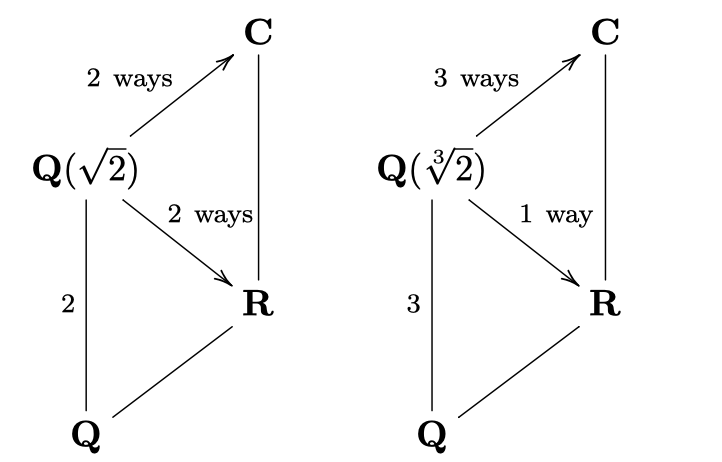
\includegraphics[width=0.5\textwidth]{Figs/4.png}
\end{figure}

\begin{exma}
To embed the field $\mathbf{Q}(\sqrt{2})$ into $\mathbf{R}$, there are \tb{two ways} this can be done: send $\sqrt{2}$ to itself or send it to $-\sqrt{2}$. That there are two embeddings is related to the fact that $X^{2}-2$ has \tb{two different roots} in $\mathbf{R}$. 
Similarly, there are \tb{two embeddings} of $\mathbf{Q}(\sqrt{2})$ into $\mathbf{C}$. 

If we try to embed $\mathbf{Q}(\sqrt[3]{2})$ into $\mathbf{R}$, there is \tb{only one way} to do this since there is only one real cube root of 2. Enlarging our target field to $\mathbf{C}$ provides us with \tb{3 different cube roots of 2} (one is real, two are non-real), so $\mathbf{Q}(\sqrt[3]{2})$ has \tb{3 different embeddings} into the complex numbers (determined by sending $\sqrt[3]{2}$ to each of the 3 cube roots of 2 in $\mathbf{C}$ ).

The number of embeddings $\mathbf{Q}(\sqrt[3]{2}) \rightarrow \mathbf{C}$ is \tb{3}, but we had to make the \tb{target field large enough} (target field $\mathbf{R}$ was too small). The number of embeddings of $\mathbf{Q}(\sqrt{2})$ and $\mathbf{Q}(\sqrt[3]{2})$ into $\mathbf{R}$ and $\mathbf{C}$ is related to the number of different roots of $X^{2}-2$ and $X^{3}-2$ in $\mathbf{R}$ and $\mathbf{C}$. That the number of roots equals the degree of each polynomial when they \tb{split completely} is related to the \tb{polynomials being separable}.
\end{exma}


We start with a lemma.
\begin{lema}\label{lem:oqnead}
We have 
\begin{enumerate}
    \item Let $\sigma: E \rightarrow E$ be an \tb{$F$-monomorphism} and assume that $f \in$ $F[X]$ \tb{splits over} $E$. Then $\sigma$ \tb{permutes} the roots of $f$, namely, \tb{if $\alpha$ is a root of $f$ in $E$ then so is $\sigma(\alpha)$.} 
    \item Similarly, Let $\sigma: E \rightarrow E'$ be an \tb{field monomorphism}, \tb{if $\alpha$ is a root of $f$ in $E$ then so is $\sigma(\alpha)$ in $E'$.} 
\end{enumerate}
 
%     \item There is a \tb{unique extension} of $\sigma: F \rightarrow F^{\prime}$ to a \tb{field isomorphism} $F(\alpha) \rightarrow F^{\prime}\left(\alpha^{\prime}\right)$ such that $\alpha \mapsto \alpha^{\prime}$. 
% \end{enumerate}

\end{lema}
\begin{proof}
Write $f(X)$ as
\begin{align*}
f(X)=b_{0}+b_{1} X+\cdots+b_{n} X^{n}, b_{i} \in F .
\end{align*}
If $\alpha$ is a root of $f$ in $E$, then
\begin{align*}
f(\alpha)=b_{0}+b_{1} \alpha+\cdots+b_{n} \alpha^{n}=0 .
\end{align*}
Apply $\sigma$ to the above equation, and use that $\sigma$ is a field homomorphism that fixes $F$ to get
\begin{align*}
b_{0}+b_{1} \sigma(\alpha)+\cdots+b_{n} \sigma(\alpha)^{n}=0,
\end{align*}
showing that $\sigma(\alpha)$ is a root.

\end{proof} 

% \begin{lema}
% There is a unique extension of $\sigma: K \rightarrow K^{\prime}$ to a field isomorphism $K(\alpha) \rightarrow K^{\prime}\left(\alpha^{\prime}\right)$ such that $\alpha \mapsto \alpha^{\prime}$. First we show uniqueness. If $\sigma^{\prime}: K(\alpha) \rightarrow K^{\prime}\left(\alpha^{\prime}\right)$ extends $\sigma$ and $\sigma^{\prime}(\alpha)=\alpha^{\prime}$, then the value of $\sigma^{\prime}$ is determined everywhere on $K(\alpha)$ because $K(\alpha)=K[\alpha]$ and
% \begin{align*}
% \sigma^{\prime}\left(\sum_{i=0}^{m} c_{i} \alpha^{i}\right)=\sum_{i=0}^{m} \sigma^{\prime}\left(c_{i}\right)\left(\sigma^{\prime}(\alpha)\right)^{i}=\sum_{i=0}^{m} \sigma\left(c_{i}\right) \alpha^{i} .
% \end{align*}
% In other words, a $K$-polynomial in $\alpha$ goes to the corresponding $K^{\prime}$-polynomial in $\alpha^{\prime}$ where $\sigma$ is applied to the coefficients. Thus there's at most one $\sigma^{\prime}$ extending $\sigma$ with $\sigma^{\prime}(\alpha)=\alpha^{\prime}$.
% \end{lema}


Let $E / F$ be a separable extension of $F$ and let $C$ be an \tb{algebraic closure} of $E$. We next count the number of \tb{$F$-monomorphisms} of $E$ into $C$ (\tb{number of embeddings} of $E$ in $C$ that \tb{fix} $F$).

\begin{thma}\label{thm:adccvrwrr}
Let $E / F$ be a \tb{finite separable extension }of degree $n$, and let $\sigma$ be an embedding of $F$ into an \tb{algebraic closure} $C$. 

Then 
\begin{enumerate}
    \item $\sigma$ extends to exactly $n$ \tb{embeddings} of $E$ in $C$. 
    \item Namely, there are exactly $n$ \tb{embeddings} $\tau$ of $E$ into $C$, such that the restriction $\left.\tau\right|_{F}$ of $\tau$ to $F$ coincides with $\sigma$.
    \item In particular, taking $\sigma$ to be the \tb{identity} on $F$, there are exactly $n$ $F$-monomorphisms of $E$ into $C$.
\end{enumerate}
\begin{figure}[h]
    \centering




\tikzset{every picture/.style={line width=0.75pt}} %set default line width to 0.75pt        

\begin{tikzpicture}[x=0.75pt,y=0.75pt,yscale=-1,xscale=1]
%uncomment if require: \path (0,300); %set diagram left start at 0, and has height of 300

%Straight Lines [id:da05336570252156991] 
\draw    (304.33,181.67) -- (304.33,119.67) ;
\draw [shift={(304.33,117.67)}, rotate = 90] [color={rgb, 255:red, 0; green, 0; blue, 0 }  ][line width=0.75]    (10.93,-3.29) .. controls (6.95,-1.4) and (3.31,-0.3) .. (0,0) .. controls (3.31,0.3) and (6.95,1.4) .. (10.93,3.29)   ;
%Straight Lines [id:da14616087535353328] 
\draw    (310.33,181.67) -- (373.88,87.33) ;
\draw [shift={(375,85.67)}, rotate = 123.96] [color={rgb, 255:red, 0; green, 0; blue, 0 }  ][line width=0.75]    (10.93,-3.29) .. controls (6.95,-1.4) and (3.31,-0.3) .. (0,0) .. controls (3.31,0.3) and (6.95,1.4) .. (10.93,3.29)   ;
%Straight Lines [id:da7865711138337743] 
\draw  [dash pattern={on 0.84pt off 2.51pt}]  (308.33,115.67) -- (370.65,76.07) ;
\draw [shift={(372.33,75)}, rotate = 147.57] [color={rgb, 255:red, 0; green, 0; blue, 0 }  ][line width=0.75]    (10.93,-3.29) .. controls (6.95,-1.4) and (3.31,-0.3) .. (0,0) .. controls (3.31,0.3) and (6.95,1.4) .. (10.93,3.29)   ;

% Text Node
\draw (299.33,184.4) node [anchor=north west][inner sep=0.75pt]    {$F$};
% Text Node
\draw (297.33,97.73) node [anchor=north west][inner sep=0.75pt]    {$E$};
% Text Node
\draw (376.67,66.4) node [anchor=north west][inner sep=0.75pt]    {$C$};
% Text Node
\draw (339.33,146.4) node [anchor=north west][inner sep=0.75pt]    {$\sigma $};
% Text Node
\draw (325.33,75.73) node [anchor=north west][inner sep=0.75pt]    {$\tau $};


\end{tikzpicture}


\end{figure}

\end{thma} 
\begin{proof}
We do a proof by induction. If $n=1$, then $E=F$ and $\sigma$ extends to exactly 1 embedding, namely itself.

We now assume that $n>1$ and choose $\alpha \in E, \alpha \notin F$. Let $f=\mu_{\alpha, F}$ be the \tb{minimal polynomial} of $\alpha$ over $F$ of degree say $r$. It is \tb{irreducible} and \tb{separable} $(E / F$ is separable by assumption). 

In order to use the induction hypothesis, we need to split the field extension $E / F$, which we do by considering the field extension $F(\alpha)$, which satisfies
\begin{align*}
E / F(\alpha) / F, [E: F(\alpha)]=n / r,[F(\alpha): F]=r .
\end{align*}
Note in the proof of \cref{thm:odmczg}, we have mentioned $F(\alpha)$ is an \tb{algebraic extension}   because  any finite extension is algebraic extension  \cref{thm:ondczfd} and $F(\alpha)$ is finite extension (\cref{thm:ienqda}). From \cref{lem:ondaee}, we further know $E / F(\alpha)$ and $F(\alpha)/F$ are \tb{separable}.

Let $\sigma$ be an embedding of $F$ into $C$, and define the polynomial $g=\sigma(f)\in \sigma(F)[X]$, where $\sigma$ is applied on all the coefficients
of $f$. The polynomial $g$ inherits the property of being \tb{irreducible} and \tb{separable} from $f$ (in the space of $\sigma(F)[X]$ not $C[X]$). 

Note, we must map $\alpha$ to one root for $g$ as mentioned in \cref{cor:odnarea}. Let $\beta$ denotes a root of $g$.  
We can thus define a \tb{unique} \tb{isomorphism} $\pi$ that maps $\alpha$ to $\beta$.
\begin{align*}
F(\alpha) &\rightarrow(\sigma(F))(\beta)\\
b_{0}+b_{1} \alpha+\ldots+b_{r} \alpha^{r} &\mapsto \sigma\left(b_{0}\right)+\sigma\left(b_{1}\right) \beta+\ldots+\sigma\left(b_{r}\right) \beta^{r}
\end{align*}
and restricted to $F$ it \tb{indeed coincides with $\sigma$.} (uniqueness is easy to see, but why there exist such a isomorphism, or say why the above is a isomorphism. Please recall the basis in \cref{thm:ienqda} and recall the same technique used in \cref{cor:odnarea})

This isomorphism is defined by the choice of $\beta$, and \tb{there are exactly $r$ choices for it, corresponding to the $r$ roots of $g$} (note that the \tb{separability} of $g$ is crucial). 

For each of these $r$ isomorphisms, using the induction hypothesis on $[E: F(\alpha)]=n / r<n$, we can extend them to exactly $n / r$ embeddings of $E$ into $C$. This gives us a total of $n / r \cdot r$ distinct embeddings of $E$ into $C$ extending $\sigma$. 
\end{proof}


% We next show a more general version of \cref{thm:adccvrwrr}. The idea is similar, but the statement is more general.
% \begin{thma}

% \end{thma}
\begin{cora}
    If $E/F$ is not separable, we have \tb{less than $n$ embeddings of $E$ in $C$.}
\end{cora}
\begin{proof}
We go through the same processing as in the prove. Then we can select one $\alpha \in E$ whose minimal polynomial has multiple roots and then the number of possible embedding is less that $r$. Consequently, we have the strictly less than $n$ embedding.
\end{proof}
\begin{cora}\label{thm:ondqeqaaa}
Let $L / F$ be a finite extension and write $L=F\left(\alpha_{1}, \ldots, \alpha_{r}\right)$. Then 

\centerline{\tb{$L / F$ is separable $\Longleftrightarrow$ each $\alpha_{i}$ is separable over $F$.}}
\end{cora} 
\begin{rema}
The usefulness of \cref{thm:ondqeqaaa} is that it gives a practical way to check a finite extension $L / F$ is separable: rather than show every element of $L$ is separable over $F$ \tb{it suffices to show there is a set of field generators for $L / F$ that are each separable over $F$.}
\end{rema}
\begin{proof}
See the supp separable1.pdf.
\end{proof}
\begin{cora}
    If $f(X) \in F[X]$ is \tb{separable} then a splitting field for $f$ over $F$ is separable over $F$.
\end{cora}
\begin{proof}
Let $L / F$ be a splitting field for $f$ over $F$. Then $L=F\left(\gamma_{1}, \ldots, \gamma_{n}\right)$ where the $\gamma_{i}$ 's are all roots of $f(X)$. Therefore the $\gamma_{i}$ 's are separable over $F$, so $L / F$ is a separable extension.
\end{proof} 



\begin{thma}\bfs{Theorem of the Primitive Element}\label{thm:d9qdadc}
If $E / F$ is a \tb{finite separable} extension, then
\begin{align*}
E=F(\gamma)
\end{align*}
for some $\gamma \in E$. We say that $\gamma$ is a \tb{primitive element} of $E$ over $F$.
\end{thma}
\begin{proof}
If $F$ is a finite field then every finite extension $L$ is a finite field. Therefore $L^{\times}$is cyclic by \cref{thm:aibrqc}. Letting $\gamma$ be a generator of $L^{\times}$, we have $L^{\times}=\langle\gamma\rangle$, so $L=F(\gamma)$.

Now consider the case when $F$ is infinite. A finite separable extension of $F$ has the form $F\left(\alpha_{1}, \ldots, \alpha_{r}\right)$ where each $\alpha_{i}$ is separable over $F$. It suffices by induction on the number of field generators to show when $F(\alpha, \beta) / F$ is separable that $F(\alpha, \beta)=F(\gamma)$ for some $\gamma$.

Let $L=F(\alpha, \beta)$ and $n=[L: F]$. Recall that a $F$-homomorphism is a homomorphism of extensions of $F$ that fixes $F$ pointwise. Since $L / F$ is separable, \cref{thm:adccvrwrr} tells us there is a field extension $C / F$ such that the number of $F$-homomorphisms $L \rightarrow C$ is $n$. Pick $c \in F$. If $F(\alpha+c \beta) \neq L$ then $[F(\alpha+c \beta): F]<[L: F]$. We will show \tb{there are only finitely many such $c$, so on account of $F$ being infinite there is a $c \in F$ such that $F(\alpha+c \beta)=L$.}

The degree $[F(\alpha+c \beta): F]$ is an upper bound on the number of $F$-homomorphisms $F(\alpha+c \beta) \rightarrow C$. Since there are $n$ $F$-homomorphisms $L \rightarrow C$, if $[F(\alpha+c \beta): F]<$ $[L: F]=n$ then there are different $F$-homomorphisms $L \rightarrow C$, say $\sigma$ and $\tau$, which are equal on $F(\alpha+c \beta)$. Therefore $\sigma \neq \tau$ on $L$ but $\sigma(\alpha+c \beta)=\tau(\alpha+c \beta)$. Then
$\sigma(\alpha)+c \sigma(\beta)=\tau(\alpha)+c \tau(\beta)$. If $\sigma(\beta)=\tau(\beta)$ then we get $\sigma(\alpha)=\tau(\alpha)$, so $\sigma=\tau$ as functions on $F(\alpha, \beta)=L$, which isn't true. Hence $\sigma(\beta) \neq \tau(\beta)$, so we can solve for $c$ :
\begin{align*}
c=\frac{\tau(\alpha)-\sigma(\alpha)}{\sigma(\beta)-\tau(\beta)} .
\end{align*}
There are only finitely many $\sigma$ and $\tau$, so only finitely many such $c$.
\end{proof}


\begin{cora}
    When $F$ has \tb{characteristic $0$}, all of its \tb{finite extensions are separable} according to \cref{cor:ibndad}, so the primitive element theorem says \tb{every finite extension field of $F$ has the form $F(\gamma)$ for some $\gamma$.}
\end{cora}
\begin{exma}
The field $\mathbf{Q}(\sqrt{2}, \sqrt{3})$ is separable over $\mathbf{Q}$ and it equals $\mathbf{Q}(\sqrt{2}+\sqrt{3})$.
\end{exma}


\subsubsection{Simple Extension}
\begin{defa}\bfs{simple extension}
A \tb{simple extension} is a field extension which is generated by the \tb{adjoining of a single element.}
\end{defa}

\begin{lema}
Thus the primitive element Theorem above provides a characterization of the finite extensions which are simple.
\end{lema}

\begin{cora}
    Number fields are simple extensions.
\end{cora}


\subsection{Normality}
\begin{enumerate}
    \item Algebraic and separable field extensions  are \tb{transitive}
    \item  We now introduce a third property, which is \tb{not transitive,} the one of being normal.
\end{enumerate}

\begin{defa}\bfs{normal, conjugate root}
\begin{enumerate}
    \item An \tb{algebraic extension} $E / F$ is \tb{normal} if every \tb{irreducible polynomial} over $F$ that has at least one root in $E$ \tb{splits} over $E$.
    \item If we call the other roots of this polynomial the \tb{conjugates} of $\alpha$, we can rephrase the definition by saying that \tb{if $\alpha \in E$, then all conjugates of $\alpha$ over $F$ are in $E$.}
\end{enumerate}
\end{defa} 
\begin{exma}
Consider the field extension $E=\mathbb{Q}(\sqrt[3]{2}) / \mathbb{Q}$. The roots of the irreducible polynomial $f(X)=X^{3}-2$ are
\begin{align*}
\sqrt[3]{2}, \zeta_{3} \sqrt[3]{2}, \zeta_{3}^{2} \sqrt[3]{2}
\end{align*}
where $\zeta_{3}$ is a primitive 3 rd root of unity (for example $\zeta_{3}=e^{2 \pi i / 3}$ ). Thus $E$ is \tb{not} a normal extension.
\end{exma} 

$\bullet$ We can give another characterization in terms of \tb{monomorphisms of $E$.}
\begin{thma}\label{thm:inaedxx}
The \tb{finite extension} $E / F$ is \tb{normal} if and only if every \tb{$F$-monomorphism} of $E$ into an \tb{algebraic closure} $C$ is actually an \tb{$F$-automorphism} of $E$. (\tb{Finite} could be replaced by \tb{algebraic}, which we will not prove).
\end{thma}
\begin{proof}
$\Rightarrow$: If $E / F$ is normal, then an $F$-monomorphism $\tau$ of $E$ into $C$ must map each element of $E$ to one of its conjugates (as is the case in the proof of \cref{lem:oqnead}). Note all elements have conjugates for some polynomial in $F[X]$. Thus $\tau(E) \subseteq E$, but $\tau(E)$ is an isomorphic copy of $E$ and thus has the \tb{same degree (i.e. dimension)} as $E$ and $E=\tau(E)$, showing that $\tau$ is indeed an ${F \text {-automorphism of } E}$.

$\Leftarrow$: Consider $\alpha \in E$ and let $\beta$ be a conjugate of $\alpha$ over $F$. There exists an $F$-monomorphism of $E$ into $C$ that carries $\alpha$ to $\beta$ (the construction is given in the proof of \cref{thm:adccvrwrr}). If all such embeddings are $F$-automorphisms of $E$, that means $\beta$ must be in $E$, and we conclude that $E / F$ is normal.
\end{proof}


$\bullet$ Here is another characterization of normal extensions in terms of \tb{splitting fields.}

\begin{thma}\label{thm:oneqdcer}
The finite extension $E / F$ is \tb{normal} if and only if $E$ is a \tb{splitting field} for some polynomial $f$ in $F[X]$.
\end{thma} 
\begin{proof}
Let $E / F$ be a finite normal extension of degree $n$, and let $\alpha_{1}, \ldots, \alpha_{n}$ be a \tb{basis} for $E$ over $F$. Consider for each $\alpha_{i}$ its minimal polynomial $f_{i}$ over $F$. By definition of normal extension, since $f_{i}$ has a root in $E$, then $f_{i}$ splits over $E$, and so does the polynomial
\begin{align*}
f=f_{1} \cdots f_{n} .
\end{align*}
To prove that $E$ is a splitting field, we are left to prove it is the smallest field over which $f$ splits. This is here that we understand why we take such an $f$. If $f$ were to split over a subfield $K$, that is $K$ such that
\begin{align*}
F \subset K \subset E
\end{align*}
then each $\alpha_{i} \in K$, and $K=E$ (this is a conclusion we cannot reach if we take for $f$ only one $f_{i}$ or a subset of them). This proves that $E$ is a splitting field for $f$ over $F$.

Conversely, let $E$ be a splitting field for some $f$ over $F$, whose roots are denoted by $\alpha_{1}, \ldots, \alpha_{n}$. Let $\tau$ be an \tb{$F$-monomorphism} of $E$ into an algebraic closure, that is $\tau$ takes each $\alpha_{i}$ into another root of $f$.

Since $E$ is a splitting field for $f$, we have
\begin{align*}
F\left(\alpha_{1}, \ldots, \alpha_{n}\right)=E
\end{align*}
and $\tau(E) \subset E$ (to see this, note $\alpha_1,\ldots,\alpha_r$ are the basis, so every elements can be linear represented using the roots). Thus since $E$ and $\tau(E)$ have same dimension, we get that
\begin{align*}
\tau(E)=E
\end{align*}
and $\tau$ is actually an \tb{automorphism} of $E$, and by the above theorem, we conclude the $E / F$ is normal.
\end{proof} 


$\bullet$ As a corollary, we see how a subextension inherits the property of normality.
\begin{cora}\label{cor:oionqdx}
Let $E / K / F$ be a finite extension $([E: F]<\infty)$. If $E / F$ is normal, so is $E / K$.
\end{cora}
\begin{proof}
Since $E / F$ is normal, $E$ is a splitting field for some polynomial $f \in F[X]$, that is $E$ is generated over $F$ by the roots of $f$. Since $f \in F[X] \subset K[X], f$ can also be seen as a polynomial in $K[X]$ and $E$ is generated over $K$ by the roots of $f$, and again by the above theorem, $E / K$ is normal.
\end{proof} 

There is no reason for an arbitrary field extension $E / F$ to be normal. However, if $E / F$ is finite (or more generally algebraic) one can always embed it in normal extension.
\begin{defa}\bfs{normal closure}
 Let $E / F$ be an \tb{algebraic extension}. The \tb{normal closure }of $E / F$ is an \tb{extension field $N$ of $E$} such that $N / E$ is \tb{normal} and $N$ is minimal with this property.
\end{defa}

\begin{exma}
If $E / F$ is finite, we can see it as follows: $E$ is finitely generated over $F$, so it can be written as $E=F\left(\alpha_{1}, \ldots, \alpha_{n}\right)$. What's the normal closure of $E/F$?

Let now $K$ be a normal extension of $F$ that contains $E$ :
\begin{align*}
K / E / F .
\end{align*}
Since $K$ is normal, it must contain not only all the $\alpha_{i}$ but also all their conjugates. Let $f_{i}$ be the minimal polynomial of $\alpha_{i}, i=1, \ldots, n$. Then we can rephrase the last statement and say that $K$ must contain all the roots of $f_{i}$, $i=1, \ldots, n$. Consider the polynomial
\begin{align*}
f=f_{1} \cdots f_{n}
\end{align*}
Let $N$ be \tb{the splitting field for $f$ over $F$} (which is unique up to isomorphism \cref{sec:ioneaddz}). Then $K$ must contain $N$.   But $N / F$ is normal from \cref{thm:oneqdcer}, so $N$ must be the smallest normal extension of $F$ that contains $E$. Thus $N$ is a \tb{normal closure of $E$ over $F$.}
\end{exma}

\subsection{Summary of Separable and Normal}
\begin{rema}
Note, in \cref{lem:qmdaadd} (note not $F$ in the lemma), we know 
\end{rema}
\begin{enumerate}
    \item Let us consider a field $K$ and let us say we fix an algebraic closure $K^{\text{alg}}$ of it.
    \begin{enumerate}
        \item Now, $K^{\text{alg}}$ might contain elements that are not separable (over $K$), that is their \tb{minimal polynomial is not a separable polynomial} (i.e., it has roots of multiplicity greater 1 in $K^{\text{alg}}$ or equivalently it is not co-prime with its derivative). This is what \cref{lem:qmdaadd} (note not $F$ in the lemma) and \cref{lem:ondzcart} are saying.
        \item Non-separable extensions and elements are not so nice in some ways (in particular sometimes we only want \tb{Galois} i.e., normal and separable). So one might consider \tb{only considering all separable (over $K$) elements} in $K^{\text{alg}}$. The collection of all these forms again a field and is called the \tb{separable closure of $K$.}
        \begin{itemize}
            \item This extension is a \tb{Galois extension} (See \cref{cor:ttqre}; In fact it is the \tb{maximal Galois extension of $K$.})
        \end{itemize}
       \item From \cref{cor:ibndad} and \cref{thm:doamra}, we have for some fields such as \tb{any field of characteristic 0} or for \tb{finite fields}, \tb{the separable closure equals the algebraic closure}. The point being that this fields are perfect fields and thus every \tb{algebraic extension is separable.}
    \end{enumerate}
    \item  \tb{Explanation of normal:} An extension $E/K$ is called normal \tb{if each irreducible polynomial in $K[X]$ that has a zero in $E$ can be decomposed into linear factors in $E$.} Or put differently, if $E$ contains one of the zeros of a polynomial $P$ it contains all the zeros of $P$. 
\end{enumerate}

\begin{lema}
Let $E$ be an algebraic extension of a field $F$. Show that the set of all elements in $E$ that are separable over $F$ forms a subfield of $E$, the \tb{separable closure of $F$ in $E$}.
\end{lema} 
\begin{proof}
From \cref{thm:ondqeqaaa}, we know if $\alpha, \beta$ are both separable over $F$, then $\alpha \pm \beta$, $\alpha \beta$, and $\alpha / \beta$. 
\end{proof}
\begin{cora}\label{cor:ttqre}
The \tb{separable closure} of $F$ in its \tb{algebraic closure} is normal.
\end{cora}
\begin{proof}
We only need to prove the conjugate roots are all in the separable closure $F^{\text{sep}}$.  For element $\alpha$ in $F^{\text{sep}}$, its minimal polynomial $P$ is separable over $F$. But then we have all the  conjugate roots are in $F^{\text{sep}}$ since they all have a minimal polynomial (factors of $P$). 
\end{proof}

\section{Galois Theory}
\subsection{Galois Group and Fixed Fields}
\subsubsection{Galois Group}
\begin{defa}\bfs{Galois Extension}
  If $E / F$ is \tb{normal} and \tb{separable}, it is said to be a \tb{Galois extension}, or alternatively, we say that $E$ is \tb{Galois over} $F$.
\end{defa}
\begin{rema}\bfs{Explanation}
\begin{enumerate}
    \item \tb{Normal} tell us the minimal polynomial of any element in $E$, say $f_\alpha$ for $\alpha\in E$, splitting over $E$.
    \item \tb{Separable} tell us the minimal polynomial of any element in $E$, say $f_\alpha$ for $\alpha\in E$, does not have repeated root over a splitting  field.
    \item So together, we need \tb{Galois extension} to have the minimal polynomial of any element in $E$, say $f_\alpha$ for $\alpha\in E$, splitting over $E$ \tb{with no repeat linear factors $X-a_i$, $a_i\in E$}.
\end{enumerate}

\end{rema}

\begin{lema}Take $E / F$ a \tb{Galois extension} of degree $n$.
\begin{enumerate}
    \item  Since it is \tb{separable} of degree $n$, we know that there are exactly $n $ \tb{$F$-monomorphisms} of $E$ into an algebraic closure $C$ (See \cref{thm:adccvrwrr}). 
    \item But $E / F$ being also \tb{normal}, every \tb{$F$-monomorphisms} into $C$ is actually an
\tb{$F$-automorphism} of $E$ (See \cref{thm:inaedxx}). 
\end{enumerate}
Thus \tb{there are exactly $n=[E: F]$ $F$-automorphisms of $E$.}
\end{lema}


We can define the notion of a Galois group for an \tb{arbitrary field extension}.
\begin{defa}\bfs{Galois group }
   If $E / F$ is a field extension, the Galois group of $E / F$, denoted by $\operatorname{Gal}(E / F)$, is the set of \tb{$F$-automorphisms} of $E$. It forms a group under the composition of functions.
\end{defa}
\begin{cora}
In a \tb{Galois extension}, the \tb{order of the Galois group} is actually the \tb{ degree of the field extension.}
\end{cora}

\begin{exma}
If $E=\mathbb{Q}(\sqrt[3]{2})$, then $\operatorname{Gal}(E / \mathbb{Q})=\{1\}$, that is the identity on $E$. But note $[E:F]=3$ since $\sqrt[3]{2}$ is the root of $X^3-2=0$.
\end{exma}

\begin{rema}
The above example illustrates the fact that though one can always define a Galois group, we need the \tb{extension to be actually Galois} to say that the \tb{order of the Galois group is actually the degree of the field extension.}
\end{rema}


\subsubsection{Fixed Fields}
\begin{defa}\bfs{fixed field; fixing group}
\begin{enumerate}
    \item Let $G=\operatorname{Gal}(E / F)$ be the \tb{Galois group} of the extension $E / F$. If $H$ is a \tb{subgroup of $G$}, the \tb{fixed field} $\mathcal{F}(H)$ of $H$, is the set of elements fixed by every \tb{automorphism in $H$}, that is
\begin{align*}
F\subseteq \mathcal{F}(H)=\{x \in E, \sigma(x)=x \text { for all } \sigma \in H\}\subseteq E
\end{align*}
\item If $K$ is an \tb{intermediate field}: $E/K/F$. Define
\begin{align*}
\mathcal{G}(K)=\operatorname{Gal}(E / K)=\{\sigma \in G, \sigma(x)=x \text { for all } x \in K\}\subseteq \operatorname{Gal}(E / F)
\end{align*}
It is the \tb{group fixing} intermediate $K$.
\end{enumerate}
\end{defa} 

Galois theory has much to do with studying the relations between \tb{fixed fields and fixing groups.}

\begin{lema}\label{lem:iqneffa}
Let $E / F$ be a \tb{finite Galois extension} with Galois group $G=$ $\operatorname{Gal}(E / F)$. Then
\begin{enumerate}
    \item The fixed field of $G$ is $F$.
    \item If $H$ is a \tb{proper subgroup} of $G$, then the fixed field $\mathcal{F}(H)$ of $H$ \tb{properly} contains $F$.
\end{enumerate}
\end{lema}
\begin{proof}
1.  Let $F_{0}$ be the fixed field of $G$ (and we have the field extensions $\left.E / F_{0} / F\right)$. We want to prove that $F_{0}=F$.

We first note that if $\sigma$ is an \tb{$F$-automorphism} of $E$ (that is $\sigma$ is in $G$ ), then by definition of $F_{0}$, $\sigma$ fixes everything in $F_{0}$, meaning that $\sigma$ is an \tb{$F_{0}$-automorphism}. Thus the $F$-automorphisms in the group $G$ coincide with the $F_{0}$-automorphisms in the group $G$.

Now we further have that \tb{$E / F_{0}$ is Galois}: indeed, we have $E / F_{0} / F$ with $E / F$ Galois thus normal and separable, and $E / F_{0}$ inherits both properties (See \cref{cor:oionqdx} and \cref{lem:ondaee}).

We now look at the degrees of the extensions considered:
\begin{align*}
\left|\operatorname{Gal}\left(E / F_{0}\right)\right|=\left[E: F_{0}\right],|\operatorname{Gal}(E / F)|=[E: F],
\end{align*}
since both are Galois. Furthermore from the above, the number of $F$- and $F_{0}$-automorphisms in $G$ coincide:
\begin{align*}
\left|\operatorname{Gal}\left(E / F_{0}\right)\right|=|\operatorname{Gal}(E / F)|
\end{align*}
showing that
\begin{align*}
\left[E: F_{0}\right]=[E: F]
\end{align*}
and by multiplicativity of the degrees
\begin{align*}
[E: F]=\left[E: F_{0}\right]\left[F_{0}: F\right] \Rightarrow\left[F_{0}: F\right]=1
\end{align*}
and $F=F_{0}$

2. In order to prove that $F \subsetneq \mathcal{F}(H)$, let us assume by contradiction that $F=\mathcal{F}(H)$

Since we consider a finite Galois extension, we can invoke the \tb{Theorem of the Primitive Element \cref{thm:d9qdadc}} and claim that
\begin{align*}
E=F(\alpha), \alpha \in E .
\end{align*}
Consider the polynomial
\begin{align*}
f(X)=\prod_{\sigma \in H}(X-\sigma(\alpha)) \in E[X] .
\end{align*}
It is a priori in $E[X]$ (because of $F$-automorphism of $E$), but we will prove now that it is actually in $F[X]$. Since by contradiction we are assuming that $F=\mathcal{F}(H)$, it is enough to proof that $f(X)$ is fixed by $H$. Indeed, take $\tau \in H$, then
\begin{align*}
\prod_{\sigma \in H}(X-\tau \sigma(\alpha))=\prod_{\sigma \in H}(X-\sigma(\alpha))
\end{align*}
since $\tau \sigma$ ranges over all $H$ as does $\sigma$.
Thus $f(X) \in F[X]$ and $f(\alpha)=0$ ( $\sigma$ must be the identity once while ranging through $H)$. Now on the one hand, we have
\begin{align*}
\operatorname{deg} f=|H|<|G|=[E: F]
\end{align*}
since we assume that $H$ is proper and $E / F$ is Galois. On the other hand,
\begin{align*}
\operatorname{deg} f \geq[F(\alpha): F]=[E: F]
\end{align*}
since $f$ is a multiple of the minimal polynomial of $\alpha$ over $F$ (equality holds if $f$ is the minimal polynomial of $\alpha$ over $F)$, and $E=F(\alpha)$. We cannot possibly have $\operatorname{deg} f<[E: F]$ and $\operatorname{deg} f \geq[E: F]$ at the same time, which is a contradiction and concludes the proof.
\end{proof}



\subsection{The Fundamental Theorem of Galois theory}
The most significant discovery of Galois is that  under some hypotheses, there is a \tb{one-to-one correspondence} between
\begin{enumerate}
    \item \tb{subgroups} of the Galois group $\operatorname{Gal}(E / F)$
    \item \tb{subfields} $M$ of $E$ such that $F \subseteq M \subseteq E$.
\end{enumerate}
The correspondence goes as follows:
\begin{itemize}
    \item To each \tb{intermediate subfield} $M$, associate the group $\operatorname{Gal}(E / M)$ of all $M$-automorphisms of $E$ :
\begin{align*}
\begin{aligned}
\mathcal{G} : \{\text { intermediate fields }\} & \rightarrow\{\text { subgroups of } \operatorname{Gal}(E / F)\} \\
M & \mapsto \mathcal{G}(M)=\operatorname{Gal}(E / M)
\end{aligned}
\end{align*}
\item To each \tb{subgroup} $H$ of $\operatorname{Gal}(E / F)$, associate the \tb{fixed subfield} $\mathcal{F}(H)$ :
\begin{align*}
\begin{aligned}
\mathcal{F}:\{\text { subgroups of } \operatorname{Gal}(E / F)\} & \rightarrow\{\text { intermediate fields }\} \\
H & \mapsto \mathcal{F}(H) .
\end{aligned}
\end{align*}
\end{itemize}


We will prove below that, under the right hypotheses, we actually have a \tb{bijection} (namely $\mathcal{G}$ is the inverse of $\mathcal{F}$ ). Let us start with an example.

\begin{exma}
Consider the field extension $E=\mathbb{Q}(i, \sqrt{5}) / \mathbb{Q}$. It has four $\mathbb{Q}$ automorphisms, given by (it is enough to describe their actions on $i$ and $\sqrt{5}$ ):
\begin{align*}
\begin{array}{ccc}
\sigma_{1}: & i \mapsto i, & \sqrt{5} \mapsto \sqrt{5} \\
\sigma_{2}: & i \mapsto-i, & \sqrt{5} \mapsto \sqrt{5} \\
\sigma_{3}: & i \mapsto i, & \sqrt{5} \mapsto-\sqrt{5} \\
\sigma_{4}: & i \mapsto-i, & \sqrt{5} \mapsto-\sqrt{5}
\end{array}
\end{align*}
thus
\begin{align*}
\operatorname{Gal}(E / \mathbb{Q})=\left\{\sigma_{1}, \sigma_{2}, \sigma_{3}, \sigma_{4}\right\}
\end{align*}
The proper subgroups of $\operatorname{Gal}(E / \mathbb{Q})$ are
\begin{align*}
\left\{\sigma_{1}\right\},\left\{\sigma_{1}, \sigma_{2}\right\},\left\{\sigma_{1}, \sigma_{3}\right\},\left\{\sigma_{1}, \sigma_{4}\right\}
\end{align*}
and their corresponding subfields are
\begin{align*}
E, \mathbb{Q}(\sqrt{5}), \mathbb{Q}(i), \mathbb{Q}(i \sqrt{5})
\end{align*}
% We thus get the following diagram:
\end{exma} 

\begin{thma}\label{thm:oqnedarr}
Let $E / F$ be a \tb{finite Galois extension} with Galois group $G$.
\begin{enumerate}
    \item The map $\mathcal{F}$ is a \tb{bijection} from \tb{subgroups} to \tb{intermediate fields}, with inverse $\mathcal{G}$.
    \item  Consider the intermediate field $K=\mathcal{F}(H)$ which is fixed by $H$, and $\sigma \in G$. Then the intermediate field
\begin{align*}
\sigma K=\{\sigma(x), x \in K\}
\end{align*}
is fixed by $\sigma H \sigma^{-1}$, namely $\sigma K=\mathcal{F}\left(\sigma H \sigma^{-1}\right)$.
\end{enumerate}
\end{thma} 
\begin{proof}
1. We first consider the composition of maps
\begin{align*}
H \rightarrow \mathcal{F}(H) \rightarrow \mathcal{G} \mathcal{F}(H)
\end{align*}
We need to prove that $\mathcal{G} \mathcal{F}(H)=H$. Take $\sigma$ in $H$, then $\sigma$ fixes $\mathcal{F}(H)$ by definition and $\sigma \in \operatorname{Gal}(E / \mathcal{F}(H))=\mathcal{G}(\mathcal{F}(H))$, showing that
\begin{align*}
H \subseteq \mathcal{G F}(H)
\end{align*}
To prove equality, we need to rule out the strict inclusion. If $H$ \tb{were a proper subgroup} of $\mathcal{G}(\mathcal{F}(H))$, by \cref{lem:iqneffa} the fixed field $\mathcal{F}(H)$ of $H$ should properly contain the fixed field of $\mathcal{G} \mathcal{F}(H)$ which is $\mathcal{F}(H)$ itself, a contradiction, showing that
\begin{align*}
H=\mathcal{G} \mathcal{F}(H) .
\end{align*}

Now consider the reverse composition of maps
\begin{align*}
K \rightarrow \mathcal{G}(K) \rightarrow \mathcal{F G}(K) .
\end{align*}
This time we need to prove that $K=\mathcal{F G}(K)$. But
\begin{align*}
\mathcal{F G}(K)=\text { fixed field by } \operatorname{Gal}(E / K)
\end{align*}
which is exactly $K$ by \cref{lem:iqneffa}.

2. It is enough to compute $\mathcal{F}\left(\sigma H \sigma^{-1}\right)$ and show that it is actually equal to $\sigma K=\sigma \mathcal{F}(H)$.
\begin{align*}
\begin{aligned}
\mathcal{F}\left(\sigma H \sigma^{-1}\right) &=\left\{x \in E, \sigma \tau \sigma^{-1}(x)=x \text { for all } \tau \in H\right\} \\
&=\left\{x \in E, \tau \sigma^{-1}(x)=\sigma^{-1}(x) \text { for all } \tau \in H\right\} \\
&=\left\{x \in E, \sigma^{-1}(x) \in \mathcal{F}(H)\right\} \\
&=\{x \in E, x \in \sigma(\mathcal{F}(H))\}=\sigma(\mathcal{F}(H))
\end{aligned}
\end{align*}
\end{proof} 
We now look at \tb{subextensions of the finite Galois extension} $E / F$ and ask about their respective Galois group.

\begin{thma}
Let $E / F$ be a \tb{finite Galois extension} with \tb{Galois group} $G$. Let $K$ be an \tb{intermediate subfield}, \tb{fixed by a subgroup $H$} according to \cref{thm:oqnedarr}. We have
\begin{enumerate}
    \item The extension $E / K$ is \tb{Galois.}
    \item The extension $K / F$ is \tb{normal} if and only if $H$ is a \tb{normal subgroup} of $G$.
    \item If $H$ is a \tb{normal subgroup} of $G$, then
    \begin{align*}
\operatorname{Gal}(K / F) \simeq G / H=\operatorname{Gal}(E / F) / \operatorname{Gal}(E / K)
\end{align*}
\item Whether $K / F$ is normal or not, we have
\begin{align*}
[K: F]=[G: H] .
\end{align*}
\end{enumerate}
\end{thma} 
\begin{proof}
1. That $E / K$ is Galois is immediate from the fact that a subextension $E / K / F$ inherits \tb{normality and separability} from $E / F$.

2. First note that $\sigma$ is an $F$-monomorphism of $K$ into $E$ (or $C$) if and only if $\sigma$ is the restriction to $K$ of an element of $G$ : 
\begin{enumerate}[a).]
    \item if $\sigma$ is an $F$-monomorphism of $K$ into $E$, it can be extended to an $F$-monomorphism of $E$ into itself thanks to the normality of $E$ (so it is the the restriction to $K$ of this $F$-monomorphism of $E$ into itself).
    \item  Conversely, if $\tau$ is an $F$-automorphism of $E$, then $\sigma=\left.\tau\right|_{K}$ is surely a $F$-monomorphism of $K$ into $E$.
\end{enumerate}
Now, by \cref{thm:inaedxx}, we have
\begin{align*}
K / F \text { normal } \Longleftrightarrow \sigma(K)=K \text { for all } \sigma \in G
\end{align*}
Note here ``for all $\sigma \in G$'' is from the above discussion.
Since $K=\mathcal{F}(H)$, we just rewrite
\begin{align*}
K / F \text { normal } \Longleftrightarrow \sigma(\mathcal{F}(H))=\mathcal{F}(H) \text { for all } \sigma \in G \text {. }
\end{align*}
Now by \cref{thm:oqnedarr}, we know that $\sigma(\mathcal{F}(H))=\mathcal{F}\left(\sigma H \sigma^{-1}\right)$, and we have
\begin{align*}
K / F \text { normal } \Longleftrightarrow \mathcal{F}\left(\sigma H \sigma^{-1}\right)=\mathcal{F}(H) \text { for all } \sigma \in G \text {. }
\end{align*}
We are almost there, we now use again the above theorem that tells us that $\mathcal{F}$ is invertible, with inverse $\mathcal{G}$, to get the conclusion:
\begin{align*}
K / F \text { normal } \Longleftrightarrow \sigma H \sigma^{-1}=H \text { for all } \sigma \in G .
\end{align*}

3. To prove this isomorphism, we will use the First Isomorphism Theorem for groups \cref{sec:dasfafdf}. Consider the group homomorphism
\begin{align*}
\operatorname{Gal}(E / F) \rightarrow \operatorname{Gal}(K / F),\left.\sigma \mapsto \sigma\right|_{K} .
\end{align*}
This map is surjective (we showed it above, when we mentioned that we can extend $\left.\sigma\right|_{K}$ to $\sigma$. Its kernel is given by
\begin{align*}
\operatorname{Ker}=\left\{\sigma,\left.\sigma\right|_{K}=1\right\}=H=\operatorname{Gal}(E / K) .
\end{align*}
Applying the First Isomorphism Theorem for groups \cref{sec:dasfafdf}, we get
\begin{align*}
\operatorname{Gal}(K / F) \simeq \operatorname{Gal}(E / F) / \operatorname{Gal}(E / K)
\end{align*}

4. Finally, by multiplicativity of the degrees:
\begin{align*}
[E: F]=[E: K][K: F] .
\end{align*}
Since $E / F$ and $E / K$ are Galois, we can rewrite
\begin{align*}
|G|=|H|[K: F] .
\end{align*}
We conclude by Lagrange Theorem:
\begin{align*}
[G: H]=|G| /|H|=[K: F] .
\end{align*}
\end{proof} 

\subsection{Finite Fields}
We will provide a precise classification of finite fields.
Theorem 7.4. Let $E$ be a finite field of characteristic $p$.
1. The cardinality of $E$ is
\begin{align*}
|E|=p^{n},
\end{align*}
for some $n \geq 1$. It is denoted $E=\mathbb{F}_{p^{n}}$.
2. Furthermore, $E$ is the splitting field for the separable polynomial
\begin{align*}
f(X)=X^{p^{n}}-X
\end{align*}
over $\mathbb{F}_{p}$, so that any finite field with $p^{n}$ elements is isomorphic to E. In fact, $E$ coincides with the set of roots of $f$.

Proof. 1. Let $\mathbb{F}_{p}$ be the finite field with $p$ elements, given by the integers modulo $p$. Since $E$ has characteristic $p$, it contains a copy of $\mathbb{F}_{p}$. Thus $E$ is a field extension of $\mathbb{F}_{p}$, and we may see $E$ as a vector space over $\mathbb{F}_{p}$. If the dimension is $n$, then let $\alpha_{1}, \ldots, \alpha_{n}$ be a basis. Every $x$ in $E$ can be written as
\begin{align*}
x=x_{1} \alpha_{1}+\cdots+x_{n} \alpha_{n}
\end{align*}
and there are $p$ choices for each $x_{i}$, thus a total of $p^{n}$ different elements in $E$.
2. Let $E^{\times}$be the multiplicative group of non-zero elements of $E$. If $\alpha \in E^{\times}$, then
\begin{align*}
\alpha^{p^{n}-1}=1
\end{align*}
by Lagrange's Theorem, so that
\begin{align*}
\alpha^{p^{n}}=\alpha
\end{align*}
for all $\alpha$ in $E$ (including $\alpha=0$ ). Thus each element of $E$ is a root of $f$, and $f$ is separable.

Now $f$ has at most $p^{n}$ distinct roots, and we have already identified the $p^{n}$ elements of $E$ as roots of $f$.

Corollary 7.5. If $E$ is a finite field of characteristic $p$, then $E / \mathbb{F}_{p}$ is a Galois extension, with cyclic Galois group, generated by the Frobenius automorphism
\begin{align*}
\sigma: x \mapsto \sigma(x)=x^{p}, x \in E .
\end{align*}
Proof. By the above proposition, we know that $E$ is a splitting field for a separable polynomial over $\mathbb{F}_{p}$, thus $E / \mathbb{F}_{p}$ is Galois.
Since $x^{p}=x$ for all $x$ in $\mathbb{F}_{p}$, we have that
\begin{align*}
\mathbb{F}_{p} \subset \mathcal{F}(\langle\sigma\rangle)
\end{align*}
that is $\mathbb{F}_{p}$ is contained in the fixed field of the cyclic subgroup generated by the Frobenius automorphism $\sigma$. But conversely, each element fixed by $\sigma$ is a root of $X^{p}-X$ so $\mathcal{F}(\langle\sigma\rangle)$ has at most $p$ elements. Consequently
\begin{align*}
\mathbb{F}_{p}=\mathcal{F}(\langle\sigma\rangle)
\end{align*}
and
\begin{align*}
\operatorname{Gal}\left(E / \mathbb{F}_{p}\right)=\langle\sigma\rangle
\end{align*}

This can be generalized when the base field is larger than $\mathbb{F}_{p}$.
Corollary 7.6. Let $E / F$ be a finite field extension with $|E|=p^{n}$ and $|F|=p^{m}$. Then $E / F$ is a Galois extension and $m \mid n$. Furthermore, the Galois group is cyclic, generated by the automorphism
\begin{align*}
\tau: x \mapsto \tau(x)=x^{p^{m}}, x \in E
\end{align*}
Proof. If the degree $[E: F]=d$, then every $x$ in $E$ can be written as
\begin{align*}
x=x_{1} \alpha_{1}+\cdots+x_{d} \alpha_{d}
\end{align*}
and there are $p^{m}$ choices for each $x_{i}$, thus a total of
\begin{align*}
\left(p^{m}\right)^{d}=p^{n}
\end{align*}
different elements in $E$, so that
\begin{align*}
d=m / n \text { and } m \mid n .
\end{align*}
The same proof as for the above corollary holds for the rest.
Thus a way to construct a finite field $E$ is, given $p$ and $n$, to construct $E=\mathbb{F}_{p^{n}}$ as a splitting field for $X^{p^{n}}-X$ over $\mathbb{F}_{p}$

Theorem 7.7. If $G$ is a finite subgroup of the multiplicative group of an arbitrary field, then $G$ is cyclic. Thus in particular, the multiplicative group $E^{\times}$of a finite field $E$ is cyclic.

Proof. The proof relies on the following fact: if $G$ is a finite abelian group, it contains an element $g$ whose order $r$ is the exponent of $G$, that is, the least common multiple of the orders of all elements of $G$.

Assuming this fact, we proceed as follows: if $x \in G$, then its order divides $r$ and thus
\begin{align*}
x^{r}=1 .
\end{align*}
Therefore each element of $G$ is a root of $X^{r}-1$ and
\begin{align*}
|G| \leq r .
\end{align*}
Conversely, $|G|$ is a multiple of the order of every element, so $|G|$ is at least as big as their least common multiple, that is
\begin{align*}
|G| \geq r
\end{align*}
and
\begin{align*}
|G|=r .
\end{align*}
Since the order of $|G|$ is $r$, and it coincides with the order of the element $g$ whose order is the exponent, we have that $G$ is generated by $g$, that is $G=\langle g\rangle$ is cyclic.

\section{Notations}
Some notations need to be unified, but in this version, for simplicity of written, I use several notation for one concept. The declare is as follows:

\begin{enumerate}
    \item Unit group: $R^*$, $\bbU$.
\end{enumerate}
\bibliographystyle{IEEEtran}
\bibliography{IEEEabrv,StringDefinitions,adv_dnn}
\end{document}
